% !TeX root = thesis.tex
\gdef\mainthesisfile{}
% !TeX root = thesis.tex
\ifdefined\UtilIncluded
  \renewcommand{\startchapter}[1]{}
  \renewcommand{\stopchapter}{}
  \renewcommand{\undefinedlabel}[2]{}
\else

\newcommand{\startchapter}[1]{\begin{document}\setcounter{chapter}{#1}\addtocounter{chapter}{-1}}
\newcommand{\stopchapter}{\printbibliography[title=Bibliography,heading=bibintoc]\end{document}}


\documentclass{book}
\usepackage[utf8]{inputenc}


\usepackage{geometry}
\geometry{
  papersize={170mm,240mm},
}

\usepackage{amsfonts,amsmath, amsthm, amssymb, mathtools}
\usepackage{xspace}
\usepackage[hidelinks,bookmarks,pdfusetitle]{hyperref}
\usepackage{listings}
\usepackage[pdftex]{graphicx}
\usepackage{bm}
\usepackage[english]{babel}
\usepackage{caption}
\usepackage{subcaption}
\usepackage[usenames,dvipsnames]{xcolor}
\usepackage{physics}
\usepackage{multicol}
\usepackage{xstring}
\usepackage{pythonhighlight}
\usepackage{parskip}
\usepackage{thmtools}
\usepackage{relsize}
\usepackage{bookmark}
\usepackage{lmodern}
\usepackage{ifthen}
\usepackage{biblatex}
\usepackage{microtype}
\usepackage{csquotes}
\usepackage{numprint}
\usepackage{mleftright}
\npthousandsep{{\ifmmode\mskip2mu\else\hskip0.2em\fi}}
\npdecimalsign{.}

\addbibresource{references.bib}

\newtheorem{theorem}{Theorem}[chapter]
\newtheorem{lemma}[theorem]{Lemma}
\newtheorem{corollary}[theorem]{Corollary}
\newtheorem{definition}[theorem]{Definition}

\DeclareRobustCommand{\oneD}{{1{\relsize{-1}D}}\xspace}
\DeclareRobustCommand{\twoD}{{2{\relsize{-1}D}}\xspace}
\DeclareRobustCommand{\threeD}{{3{\relsize{-1}D}}\xspace}
\DeclareRobustCommand{\cpp}{{{C\nolinebreak[4]\hspace{-.05em}\raisebox{.4ex}{\relsize{-3}\textbf{++}}}\xspace}}
\pdfstringdefDisableCommands{%
  \def\cpp{C++}%
  \def\oneD{1D}%
  \def\twoD{2D}%
  \def\threeD{3D}%
}

\newcommand{\longchapter}[2][]{%
  \chapter[#2]{#2}%
  \ifthenelse{\equal{#1}{}}{}{\chaptermark{#1}}}

\newcommand{\NN}{\mathbb{N}}
\newcommand{\ZZ}{\mathbb{Z}}
\newcommand{\QQ}{\mathbb{Q}}
\newcommand{\QQbar}{\overline{\mathbb{Q}}}
\newcommand{\RR}{\mathbb{R}}
\newcommand{\CC}{\mathbb{C}}

\newcommand{\Eigen}{\texttt{Eigen}}

\newcommand{\sage}{\texttt{sage}\xspace}

\newcommand{\hamiltonian}{\mathcal{H}}

\newcommand{\transposesign}{\intercal}
\newcommand{\transpose}[1]{{#1}^\transposesign}
\newcommand{\adjointsign}{\text{H}}
\newcommand{\adjoint}[1]{{#1}^\adjointsign}

\newcommand{\xmin}{{x_{\text{min}}}}
\newcommand{\xmax}{{x_{\text{max}}}}
\newcommand{\ymin}{{y_{\text{min}}}}
\newcommand{\ymax}{{y_{\text{max}}}}

\newcommand{\Cbottom}{\vb{C}_\text{bottom}}
\newcommand{\Ctop}{\vb{C}_\text{top}}
\newcommand{\ubottom}{\vb{u}_\text{bottom}}
\newcommand{\utop}{\vb{u}_\text{top}}

\DeclareMathOperator{\diag}{diag}
\DeclareMathOperator{\tridiag}{tridiag}
\DeclareMathOperator{\eigs}{eigs}
\DeclareMathOperator*{\argmin}{arg\,min}
\DeclareMathOperator{\Ai}{Ai}
\DeclareMathOperator{\Bi}{Bi}
\DeclareMathOperator{\OO}{\mathcal{O}}

% https://tex.stackexchange.com/a/18192/163747
\makeatletter
\newcommand{\undefinedlabel}[2]{%
  \protected@write \@auxout {}{\string \newlabel {#1}{{#2}{\thepage}{#2}{#1}{}} }%
  \hypertarget{#1}{}
}
\makeatother

\fi
\gdef\UtilIncluded{}



\title{Algorithms for time-independent Schrödinger equations}
\author{Toon Baeyens}

\begin{document}

% !TeX root = thesis.tex
% LTeX: enabled=false
\newgeometry{right=32mm, bottom=20mm}
\begin{titlepage}
    \AddToShipoutPicture*{
        \put(0,0){%
            \parbox[b][\paperheight]{\paperwidth}{%
                \hfill\scalebox{-1}[1]{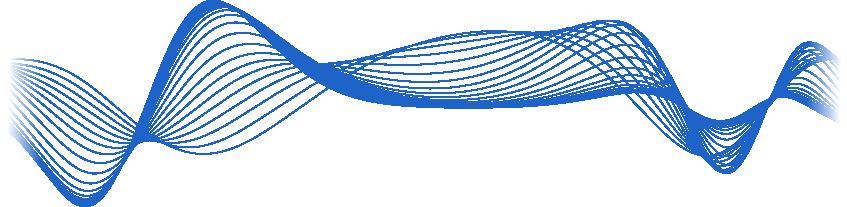
\includegraphics[width=\paperheight,height=4cm,angle=90]{img/titlepage/background_clean.pdf}}\hspace{5mm}
            }}}


    \begin{minipage}{6cm}
        \begin{flushleft}
            \relsize{-1}
            Department of Applied Mathematics, \\
            Computer Science and Statistics

            \vspace{3mm}

            {\relsize{+1}Faculty of Sciences}
        \end{flushleft}
    \end{minipage}

    \vspace{35mm}

    \begin{center}
        {\fontfamily{qag}\selectfont
            \textbf{\relsize{+4} Algorithms for time-independent\\\vspace{3mm}Schrödinger equations}
        }

        \vspace{6mm}

        \textbf{\relsize{+1} Toon Baeyens}

    \end{center}

    \vspace{1cm}

    \begin{center}
        {\relsize{-1}Supervisors} \\\vspace{1mm}
        \begin{minipage}{45mm}
            prof.\ dr.\ Marnix Van Daele

            prof.\ dr.\ Joris Van der Jeugt
        \end{minipage}
    \end{center}

    \vfill

    \begin{flushleft}
        \relsize{-1}
        Dissertation submitted in partial fulfillment\\
        of the requirements for the degree of \\
        Doctor of Science: Mathematics\\\vspace{3mm}
        June 2023
    \end{flushleft}

    \vspace{0cm}

    \begin{center}
    \end{center}

    \begin{minipage}{5cm}
        \hspace{-1cm}
\includegraphics[width=5cm]{img/logo_ugent.pdf}
    \end{minipage}%
    \hfill%

\end{titlepage}
\restoregeometry
% LTeX: enabled=true


\chapter*{Table of contents}
\addcontentsline{toc}{chapter}{Table of contents}
\markboth{Table of contents}{Table of contents}
\makeatletter
\@starttoc{toc}
\makeatother

% !TeX root = chapter_preface.tex
% !TeX root = thesis.tex
\ifdefined\UtilIncluded
  \renewcommand{\startchapter}[1]{}
  \renewcommand{\stopchapter}{}
  \renewcommand{\undefinedlabel}[2]{}
\else

\newcommand{\startchapter}[1]{\begin{document}\setcounter{chapter}{#1}\addtocounter{chapter}{-1}}
\newcommand{\stopchapter}{\printbibliography[title=Bibliography,heading=bibintoc]\end{document}}


\documentclass{book}
\usepackage[utf8]{inputenc}


\usepackage{geometry}
\geometry{
  papersize={170mm,240mm},
}

\usepackage{amsfonts,amsmath, amsthm, amssymb, mathtools}
\usepackage{xspace}
\usepackage[hidelinks,bookmarks,pdfusetitle]{hyperref}
\usepackage{listings}
\usepackage[pdftex]{graphicx}
\usepackage{bm}
\usepackage[english]{babel}
\usepackage{caption}
\usepackage{subcaption}
\usepackage[usenames,dvipsnames]{xcolor}
\usepackage{physics}
\usepackage{multicol}
\usepackage{xstring}
\usepackage{pythonhighlight}
\usepackage{parskip}
\usepackage{thmtools}
\usepackage{relsize}
\usepackage{bookmark}
\usepackage{lmodern}
\usepackage{ifthen}
\usepackage{biblatex}
\usepackage{microtype}
\usepackage{csquotes}
\usepackage{numprint}
\usepackage{mleftright}
\npthousandsep{{\ifmmode\mskip2mu\else\hskip0.2em\fi}}
\npdecimalsign{.}

\addbibresource{references.bib}

\newtheorem{theorem}{Theorem}[chapter]
\newtheorem{lemma}[theorem]{Lemma}
\newtheorem{corollary}[theorem]{Corollary}
\newtheorem{definition}[theorem]{Definition}

\DeclareRobustCommand{\oneD}{{1{\relsize{-1}D}}\xspace}
\DeclareRobustCommand{\twoD}{{2{\relsize{-1}D}}\xspace}
\DeclareRobustCommand{\threeD}{{3{\relsize{-1}D}}\xspace}
\DeclareRobustCommand{\cpp}{{{C\nolinebreak[4]\hspace{-.05em}\raisebox{.4ex}{\relsize{-3}\textbf{++}}}\xspace}}
\pdfstringdefDisableCommands{%
  \def\cpp{C++}%
  \def\oneD{1D}%
  \def\twoD{2D}%
  \def\threeD{3D}%
}

\newcommand{\longchapter}[2][]{%
  \chapter[#2]{#2}%
  \ifthenelse{\equal{#1}{}}{}{\chaptermark{#1}}}

\newcommand{\NN}{\mathbb{N}}
\newcommand{\ZZ}{\mathbb{Z}}
\newcommand{\QQ}{\mathbb{Q}}
\newcommand{\QQbar}{\overline{\mathbb{Q}}}
\newcommand{\RR}{\mathbb{R}}
\newcommand{\CC}{\mathbb{C}}

\newcommand{\Eigen}{\texttt{Eigen}}

\newcommand{\sage}{\texttt{sage}\xspace}

\newcommand{\hamiltonian}{\mathcal{H}}

\newcommand{\transposesign}{\intercal}
\newcommand{\transpose}[1]{{#1}^\transposesign}
\newcommand{\adjointsign}{\text{H}}
\newcommand{\adjoint}[1]{{#1}^\adjointsign}

\newcommand{\xmin}{{x_{\text{min}}}}
\newcommand{\xmax}{{x_{\text{max}}}}
\newcommand{\ymin}{{y_{\text{min}}}}
\newcommand{\ymax}{{y_{\text{max}}}}

\newcommand{\Cbottom}{\vb{C}_\text{bottom}}
\newcommand{\Ctop}{\vb{C}_\text{top}}
\newcommand{\ubottom}{\vb{u}_\text{bottom}}
\newcommand{\utop}{\vb{u}_\text{top}}

\DeclareMathOperator{\diag}{diag}
\DeclareMathOperator{\tridiag}{tridiag}
\DeclareMathOperator{\eigs}{eigs}
\DeclareMathOperator*{\argmin}{arg\,min}
\DeclareMathOperator{\Ai}{Ai}
\DeclareMathOperator{\Bi}{Bi}
\DeclareMathOperator{\OO}{\mathcal{O}}

% https://tex.stackexchange.com/a/18192/163747
\makeatletter
\newcommand{\undefinedlabel}[2]{%
  \protected@write \@auxout {}{\string \newlabel {#1}{{#2}{\thepage}{#2}{#1}{}} }%
  \hypertarget{#1}{}
}
\makeatother

\fi
\gdef\UtilIncluded{}


\startchapter{0}

\undefinedlabel{cha:c1}{1}
\undefinedlabel{cha:c2}{2}
\undefinedlabel{cha:c3}{3}
\undefinedlabel{cha:c4}{4}

\chapter*{Preface}
\addcontentsline{toc}{chapter}{Preface}
\markboth{Preface}{Preface}

A thesis is a work of long breath\footnote{This is a literal translation of the Dutch expression: `\foreignlanguage{dutch}{Een werk van lange adem}'.}. During the past five years, I have worked on this project. In this book you can find my process in learning about and contributing to the numerical study of Schrödinger equations.

This thesis is written from quite a technical perspective and is definitely not suited as an introductory text to the subject. Following along will require quite a lot of background knowledge. The text assumes you are already familiar with (partial) differential equations, numerical methods for solving these and the intricacies when implementing them. If you want to know \emph{all} advances written in this work, then reading the book cover to cover may be the best way. I tried to logically structure the work with sufficient cross-references and citations.

If however you are still interested in reading this book without a deep technical knowledge, then I recommend skipping the more technical discussions. Starting with the summary will provide you with a basic overview about what you can expect from this work. Chapter~\ref{cha:c1} gives some historical context about mathematical evolution and in particular about the conception of differential equations. Chapters~\ref{cha:c2},~\ref{cha:c3} and~\ref{cha:c4} contain the innovations from this thesis. Each of these chapters starts with some historical background and mathematical motivation, and ends with some numerical experiments to evaluate the performance (both in accuracy as efficiency) of our methods. For simply a cursory examination of my research, these first and last sections may be sufficient.

If you are still interested in this thesis, however not so much in the mathematics, even then I can provide some guidance on how to read it. I assume you are more interested in doing research in general or even in me personally. In this case you may\footnote{Of course, as the owner of a book you can read it however you want (or even burn it). So, not that you need it, but you definitely have my permission to skip (large) parts, if they are not of interest to you.} just skip chapters~\ref{cha:c2},~\ref{cha:c3} and~\ref{cha:c4} entirely. The summary and chapter~\ref{cha:c1} may provide sufficient context. For some personal notes, I recommend taking a look at the closing remarks at the end of this work as well.

In the introductory paragraph I stated that this research came into fruition within the past five years. In the most literal sense, this is of course true. Practically however, doing research is quite an individual pursuit, and as such it is quite a personal one. Each researcher is different and experiences the world around them uniquely. This difference, in part, relies on the background of the (mathematical) education of the researcher. In my case, I think I can say that my `mathematical career' started a good fifteen years ago. My interest in and passion for mathematics became abundantly clear\footnote{To the detriment of the non-science courses.} throughout high school. My mathematical adventure really took off when I started at Ghent University. Now, ten years later, I can close this chapter with the completion of a PhD in mathematics.


\section*{Acknowledgement}
\addcontentsline{toc}{section}{Acknowledgement}

Even though doing research is quite a lonely process, I was never alone. There are many people who let me find myself and helped me grow. Here I want to seize the opportunity to thank them wholeheartedly.

First and foremost I want to thank my very best friend. Emilie has always\footnote{At least, as long as I can remember.} been here for me. Without her, even survival would be difficult. She encourages me to pursue all my dreams and ambitions, she possesses the curiosity to listen to all my ramblings, and she understands me. Maybe not so much when I am saying nonsense, but even then she understands \emph{me}. She has the same wandering mind as mine, only in a uniquely different way. She broadens my horizons and is not afraid to tell me when I am wrong\footnote{I have absolutely no problem admitting when I am wrong. I believe my challenge is to \emph{see} when I am wrong.}. \emph{\foreignlanguage{dutch}{Lieve Floe, dank je wel; een eenvoudige, toch zeer diepe en welgemeende ``Dank je.''.}}

Concerning the content of this work, Marnix has been invaluable. As a promotor, he was a true guide. He gave me all the tools necessary during this research. He granted me the freedom to explore \emph{all}\footnote{This is not an exaggeration. I am extremely grateful that he never told me ``no'', he never instructed me to manage my time differently.} my ideas and side projects. At times, he even poured gasoline on the fire by encouraging me to create some unimaginably beautiful images. Nonetheless, he always guided me back. Marnix kept motivating me to write down my ideas into articles, and he was rightly critical about my first drafts. As an example, my first draft of chapter~\ref{cha:c4} (now 54 pages) was a mere two pages of only mathematical notation, without context. As my copromotor, I also thank Joris. When communication stalled, with only a few words, he got everything back on track.

As stated earlier, while researching and learning new things I depend on my background. Thanks to my parents and family, this is such a rich background. \emph{\foreignlanguage{dutch}{Mama, Papa, dank je wel. Dank je, om me alle ruimte te geven om zelf op zoek te gaan, om in me te geloven en me te steunen. Dank je wel dat ik in Sinaai steeds een plek zal hebben om thuis te komen. Natuurlijk dank ik ook Wannes en Kaat, om mij te leren dat ik nooit alleen ben. Dank je, aan de hele uitgebreide familie voor zoveel adressen waar ik steeds een warme plek kan vinden.}}

With much pleasure I want to thank my youngest friend. In all honesty, Ward should be a co-author of this work. We have spent many hours writing together. Most of the time, I was wielding the keyboard. However, he also undoubtedly contributed. If you find some stray letters throughout this text, chances are these were written by a very curious and extremely enthusiastic one-and-a-half year old.

I am fortunate to be able to say: throughout the last years many friends became colleagues, and many colleagues became friends.

There are new friends, who first were colleagues. In particular, I thank Annick, Asmus, Bart, Dieter, Heidi, Jonathan, Louise, Nico, Niko, Oliver, Pieter, Rien, Robbert, Roy, Tibo, and Tom for giving me the joy of going to work, day in and day out. Coming into the office has always been a pleasure by being greeted by the ``Good morning!'''s of Camilla, Felix, Jorg, Niels, Pieter, and Wout. There are even a few colleagues, who I now dare to call dear friends. I wholeheartedly thank Alexis for taking the time (during a very busy period) to thoroughly read my whole thesis and providing invaluable comments like `Pew pew!' every time the `shooting' technique was mentioned. I also thank Steven for being a companion in discovering new mathematics, solving many problems, and exploring the deep caverns of the \cpp{} specification. And of course, I thank Charlotte. It still astonishes me how opposite we are, and yet so similar. Thank you for fighting all our battles with me, always side-by-side, never head-to-head. 

And there are old friends. People who have grown with me for already a decade and more. In particular, I thank my fellow students Wouter, Frederik, Sam, and David. And I thank Bart and Jorn for their long-lasting friendships, our dates are as valuable as they are scarce. All of you have helped me become the mathematician I am today, however some in particular contributed a great deal to the person I am today. I thank Hadewijch for all the pancakes, all the (late-night) talks, and all the adventurous double-dates which still await us. I thank Simon, for motivating me with chocolate waffles, for letting me sometimes win with Beatsaber, and for the many level-headed much-needed conversations. And, I thank Jens for all his creativity, for first saying yes and then doubting if it may have been too ambitious, and for his courage to do what he loves. 

Last but definitely not least I want to thank my jury. Liviu, Guido, Veerle, Kris and Dajana, thank you for taking the time to read my work with such interest. In particular, I thank Liviu for providing many of the building blocks needed in this work, for his hospitality in inviting us to Sinaia, and for his many comments and suggestions.

\section*{Closing the opening words}

To end this section there is still one person left to thank, and that is you: the reader. Writing this book has been quite the adventure, and I hope reading it will give you a sincere view on the whole affair.

If you have any questions, remarks or comments (about this work, or even more generally about me), I am very eager to hear them. Please do reach out!

Finally, I wish you the very best of luck in reading this thesis.


\begin{flushright}
    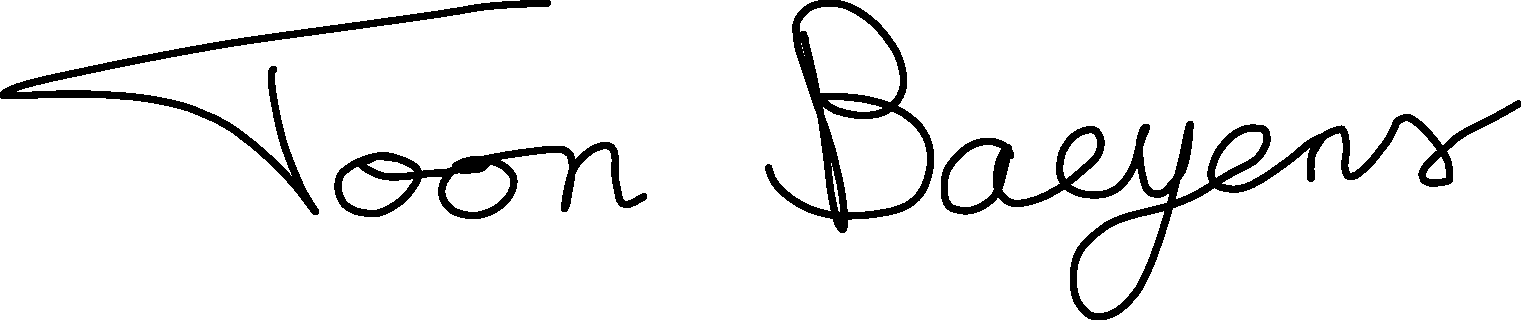
\includegraphics[width=4cm]{img/signature.pdf}\\
    June 2023
\end{flushright}

\stopchapter


% !TeX root = chapter_software.tex
% !TeX root = thesis.tex
\ifdefined\UtilIncluded
  \renewcommand{\startchapter}[1]{}
  \renewcommand{\stopchapter}{}
  \renewcommand{\undefinedlabel}[2]{}
\else

\newcommand{\startchapter}[1]{\begin{document}\setcounter{chapter}{#1}\addtocounter{chapter}{-1}}
\newcommand{\stopchapter}{\printbibliography[title=Bibliography,heading=bibintoc]\end{document}}


\documentclass{book}
\usepackage[utf8]{inputenc}


\usepackage{geometry}
\geometry{
  papersize={170mm,240mm},
}

\usepackage{amsfonts,amsmath, amsthm, amssymb, mathtools}
\usepackage{xspace}
\usepackage[hidelinks,bookmarks,pdfusetitle]{hyperref}
\usepackage{listings}
\usepackage[pdftex]{graphicx}
\usepackage{bm}
\usepackage[english]{babel}
\usepackage{caption}
\usepackage{subcaption}
\usepackage[usenames,dvipsnames]{xcolor}
\usepackage{physics}
\usepackage{multicol}
\usepackage{xstring}
\usepackage{pythonhighlight}
\usepackage{parskip}
\usepackage{thmtools}
\usepackage{relsize}
\usepackage{bookmark}
\usepackage{lmodern}
\usepackage{ifthen}
\usepackage{biblatex}
\usepackage{microtype}
\usepackage{csquotes}
\usepackage{numprint}
\usepackage{mleftright}
\npthousandsep{{\ifmmode\mskip2mu\else\hskip0.2em\fi}}
\npdecimalsign{.}

\addbibresource{references.bib}

\newtheorem{theorem}{Theorem}[chapter]
\newtheorem{lemma}[theorem]{Lemma}
\newtheorem{corollary}[theorem]{Corollary}
\newtheorem{definition}[theorem]{Definition}

\DeclareRobustCommand{\oneD}{{1{\relsize{-1}D}}\xspace}
\DeclareRobustCommand{\twoD}{{2{\relsize{-1}D}}\xspace}
\DeclareRobustCommand{\threeD}{{3{\relsize{-1}D}}\xspace}
\DeclareRobustCommand{\cpp}{{{C\nolinebreak[4]\hspace{-.05em}\raisebox{.4ex}{\relsize{-3}\textbf{++}}}\xspace}}
\pdfstringdefDisableCommands{%
  \def\cpp{C++}%
  \def\oneD{1D}%
  \def\twoD{2D}%
  \def\threeD{3D}%
}

\newcommand{\longchapter}[2][]{%
  \chapter[#2]{#2}%
  \ifthenelse{\equal{#1}{}}{}{\chaptermark{#1}}}

\newcommand{\NN}{\mathbb{N}}
\newcommand{\ZZ}{\mathbb{Z}}
\newcommand{\QQ}{\mathbb{Q}}
\newcommand{\QQbar}{\overline{\mathbb{Q}}}
\newcommand{\RR}{\mathbb{R}}
\newcommand{\CC}{\mathbb{C}}

\newcommand{\Eigen}{\texttt{Eigen}}

\newcommand{\sage}{\texttt{sage}\xspace}

\newcommand{\hamiltonian}{\mathcal{H}}

\newcommand{\transposesign}{\intercal}
\newcommand{\transpose}[1]{{#1}^\transposesign}
\newcommand{\adjointsign}{\text{H}}
\newcommand{\adjoint}[1]{{#1}^\adjointsign}

\newcommand{\xmin}{{x_{\text{min}}}}
\newcommand{\xmax}{{x_{\text{max}}}}
\newcommand{\ymin}{{y_{\text{min}}}}
\newcommand{\ymax}{{y_{\text{max}}}}

\newcommand{\Cbottom}{\vb{C}_\text{bottom}}
\newcommand{\Ctop}{\vb{C}_\text{top}}
\newcommand{\ubottom}{\vb{u}_\text{bottom}}
\newcommand{\utop}{\vb{u}_\text{top}}

\DeclareMathOperator{\diag}{diag}
\DeclareMathOperator{\tridiag}{tridiag}
\DeclareMathOperator{\eigs}{eigs}
\DeclareMathOperator*{\argmin}{arg\,min}
\DeclareMathOperator{\Ai}{Ai}
\DeclareMathOperator{\Bi}{Bi}
\DeclareMathOperator{\OO}{\mathcal{O}}

% https://tex.stackexchange.com/a/18192/163747
\makeatletter
\newcommand{\undefinedlabel}[2]{%
  \protected@write \@auxout {}{\string \newlabel {#1}{{#2}{\thepage}{#2}{#1}{}} }%
  \hypertarget{#1}{}
}
\makeatother

\fi
\gdef\UtilIncluded{}


\startchapter{0}

\undefinedlabel{cha:c2}{2}
\undefinedlabel{cha:c3}{3}
\undefinedlabel{cha:c4}{4}

\chapter*{Summary}
\addcontentsline{toc}{chapter}{Summary}


\section*{English summary}
\addcontentsline{toc}{section}{English summary}

An $n$-dimensional time-independent Schrödinger equation is a linear second order partial differential equation given by
\begin{equation}\label{equ:sum_en_schrodinger}
-\nabla^2 \psi(\vb{x}) + V(\vb{x}) \psi(\vb{x}) = E\vb{x}\text{.}
\end{equation}
In this expression, $V$ is a provided potential functions defined on the domain $\Omega \subseteq \RR^n$. When solving this equation, the goal is to find all functions $\psi : \Omega \to \RR$ and values $E \in \RR$ that satisfy the Schrödinger equation~\eqref{equ:sum_en_schrodinger} in combination with provided boundary conditions. In such a solution $E$ is called the eigenvalue, with corresponding eigenfunction $\psi$.

For the one-dimensional case, Schrödinger equations are a special case of Sturm--Liouville equations:
\begin{equation}\label{equ:sum_en_sl}
    -(p(x), y'(x))' + q(x) y(x) = \lambda w(x) y(x) \text{.}
\end{equation}
In this equation $p(x)$, $q(x)$ and $w(x)$ are given functions on a connected domain $[a, b] \subseteq \RR$. Here, $\lambda$ is the unknown eigenvalue with corresponding eigenfunction $y$.

In chapter \ref{cha:c2}, an existing numerical method for approximating eigenvalues and eigenfunctions of \eqref{equ:sum_en_sl} is studied. Here regular Sturm--Liouville problems on $[a, b]$ are considered with homogeneous Robin boundary conditions:
$$
\alpha_a y(a) + \beta_a p(a) y'(a) = 0 \text{ and } \alpha_b y(b) + \beta_b p(b) y'(b) = 0\text{.}
$$
This constant-perturbation method is able to reach extremely accurate results, for small as well as high eigenvalues.

\todo{Why is ours better?}

\todo{Two-dimensional problems.}

% LTeX: language=nl-BE
\section*{Nederlandse samenvatting}
\addcontentsline{toc}{section}{Nederlandse samenvatting}


\stopchapter


% !TeX root = chapter_software.tex
% !TeX root = thesis.tex
\ifdefined\UtilIncluded
  \renewcommand{\startchapter}[1]{}
  \renewcommand{\stopchapter}{}
  \renewcommand{\undefinedlabel}[2]{}
\else

\newcommand{\startchapter}[1]{\begin{document}\setcounter{chapter}{#1}\addtocounter{chapter}{-1}}
\newcommand{\stopchapter}{\printbibliography[title=Bibliography,heading=bibintoc]\end{document}}


\documentclass{book}
\usepackage[utf8]{inputenc}


\usepackage{geometry}
\geometry{
  papersize={170mm,240mm},
}

\usepackage{amsfonts,amsmath, amsthm, amssymb, mathtools}
\usepackage{xspace}
\usepackage[hidelinks,bookmarks,pdfusetitle]{hyperref}
\usepackage{listings}
\usepackage[pdftex]{graphicx}
\usepackage{bm}
\usepackage[english]{babel}
\usepackage{caption}
\usepackage{subcaption}
\usepackage[usenames,dvipsnames]{xcolor}
\usepackage{physics}
\usepackage{multicol}
\usepackage{xstring}
\usepackage{pythonhighlight}
\usepackage{parskip}
\usepackage{thmtools}
\usepackage{relsize}
\usepackage{bookmark}
\usepackage{lmodern}
\usepackage{ifthen}
\usepackage{biblatex}
\usepackage{microtype}
\usepackage{csquotes}
\usepackage{numprint}
\usepackage{mleftright}
\npthousandsep{{\ifmmode\mskip2mu\else\hskip0.2em\fi}}
\npdecimalsign{.}

\addbibresource{references.bib}

\newtheorem{theorem}{Theorem}[chapter]
\newtheorem{lemma}[theorem]{Lemma}
\newtheorem{corollary}[theorem]{Corollary}
\newtheorem{definition}[theorem]{Definition}

\DeclareRobustCommand{\oneD}{{1{\relsize{-1}D}}\xspace}
\DeclareRobustCommand{\twoD}{{2{\relsize{-1}D}}\xspace}
\DeclareRobustCommand{\threeD}{{3{\relsize{-1}D}}\xspace}
\DeclareRobustCommand{\cpp}{{{C\nolinebreak[4]\hspace{-.05em}\raisebox{.4ex}{\relsize{-3}\textbf{++}}}\xspace}}
\pdfstringdefDisableCommands{%
  \def\cpp{C++}%
  \def\oneD{1D}%
  \def\twoD{2D}%
  \def\threeD{3D}%
}

\newcommand{\longchapter}[2][]{%
  \chapter[#2]{#2}%
  \ifthenelse{\equal{#1}{}}{}{\chaptermark{#1}}}

\newcommand{\NN}{\mathbb{N}}
\newcommand{\ZZ}{\mathbb{Z}}
\newcommand{\QQ}{\mathbb{Q}}
\newcommand{\QQbar}{\overline{\mathbb{Q}}}
\newcommand{\RR}{\mathbb{R}}
\newcommand{\CC}{\mathbb{C}}

\newcommand{\Eigen}{\texttt{Eigen}}

\newcommand{\sage}{\texttt{sage}\xspace}

\newcommand{\hamiltonian}{\mathcal{H}}

\newcommand{\transposesign}{\intercal}
\newcommand{\transpose}[1]{{#1}^\transposesign}
\newcommand{\adjointsign}{\text{H}}
\newcommand{\adjoint}[1]{{#1}^\adjointsign}

\newcommand{\xmin}{{x_{\text{min}}}}
\newcommand{\xmax}{{x_{\text{max}}}}
\newcommand{\ymin}{{y_{\text{min}}}}
\newcommand{\ymax}{{y_{\text{max}}}}

\newcommand{\Cbottom}{\vb{C}_\text{bottom}}
\newcommand{\Ctop}{\vb{C}_\text{top}}
\newcommand{\ubottom}{\vb{u}_\text{bottom}}
\newcommand{\utop}{\vb{u}_\text{top}}

\DeclareMathOperator{\diag}{diag}
\DeclareMathOperator{\tridiag}{tridiag}
\DeclareMathOperator{\eigs}{eigs}
\DeclareMathOperator*{\argmin}{arg\,min}
\DeclareMathOperator{\Ai}{Ai}
\DeclareMathOperator{\Bi}{Bi}
\DeclareMathOperator{\OO}{\mathcal{O}}

% https://tex.stackexchange.com/a/18192/163747
\makeatletter
\newcommand{\undefinedlabel}[2]{%
  \protected@write \@auxout {}{\string \newlabel {#1}{{#2}{\thepage}{#2}{#1}{}} }%
  \hypertarget{#1}{}
}
\makeatother

\fi
\gdef\UtilIncluded{}


\startchapter{0}

\undefinedlabel{cha:c2}{2}
\undefinedlabel{cha:c3}{3}
\undefinedlabel{cha:c4}{4}

\chapter*{Developed software}
\addcontentsline{toc}{chapter}{Overview of developed software}

All developed software consists out of \cpp{}-source files together with a \lpython{}-packages. This \lpython{}-package provides a user-friendly interface to the efficiently implemented \cpp{}-code. To build upon this code, \lpython{} is an optional dependency. All Schrödinger problems can also be expressed using only \cpp{}.

\subsection*{Matslise 3.0 --- pyslise}

Solving one-dimensional Sturm--Liouville and Schrödinger problems with homogenous Robin or periodic boundary conditions. See chapter~\ref{cha:c2}.

\url{https://github.com/twist-numerical/matslise} \\
\url{https://pypi.org/project/pyslise/}


\subsection*{Matslise 2D --- pyslise2d}

Approximating eigenvalues and eigenfunctions of two-dimensional Schrödinger problems on rectangular domains with homogenous Dirichlet boundary conditions, using the method from chapter~\ref{cha:c3}.

\url{https://github.com/twist-numerical/matslise2d} \\
\url{https://pypi.org/project/pyslise2d/}


\subsection*{Strands --- strands}

Approximating eigenvalues and eigenfunctions of two-dimensional Schrödinger problems on general bounded domains with homogenous Dirichlet boundary conditions, using the method from chapter~\ref{cha:c4}.

\url{https://github.com/twist-numerical/strands} \\
\url{https://pypi.org/project/Strands/}


\stopchapter


% !TeX root = chapter1_introduction.tex
% !TeX root = thesis.tex
\ifdefined\UtilIncluded
  \renewcommand{\startchapter}[1]{}
  \renewcommand{\stopchapter}{}
  \renewcommand{\undefinedlabel}[2]{}
\else

\newcommand{\startchapter}[1]{\begin{document}\setcounter{chapter}{#1}\addtocounter{chapter}{-1}}
\newcommand{\stopchapter}{\printbibliography[title=Bibliography,heading=bibintoc]\end{document}}


\documentclass{book}
\usepackage[utf8]{inputenc}


\usepackage{geometry}
\geometry{
  papersize={170mm,240mm},
}

\usepackage{amsfonts,amsmath, amsthm, amssymb, mathtools}
\usepackage{xspace}
\usepackage[hidelinks,bookmarks,pdfusetitle]{hyperref}
\usepackage{listings}
\usepackage[pdftex]{graphicx}
\usepackage{bm}
\usepackage[english]{babel}
\usepackage{caption}
\usepackage{subcaption}
\usepackage[usenames,dvipsnames]{xcolor}
\usepackage{physics}
\usepackage{multicol}
\usepackage{xstring}
\usepackage{pythonhighlight}
\usepackage{parskip}
\usepackage{thmtools}
\usepackage{relsize}
\usepackage{bookmark}
\usepackage{lmodern}
\usepackage{ifthen}
\usepackage{biblatex}
\usepackage{microtype}
\usepackage{csquotes}
\usepackage{numprint}
\usepackage{mleftright}
\npthousandsep{{\ifmmode\mskip2mu\else\hskip0.2em\fi}}
\npdecimalsign{.}

\addbibresource{references.bib}

\newtheorem{theorem}{Theorem}[chapter]
\newtheorem{lemma}[theorem]{Lemma}
\newtheorem{corollary}[theorem]{Corollary}
\newtheorem{definition}[theorem]{Definition}

\DeclareRobustCommand{\oneD}{{1{\relsize{-1}D}}\xspace}
\DeclareRobustCommand{\twoD}{{2{\relsize{-1}D}}\xspace}
\DeclareRobustCommand{\threeD}{{3{\relsize{-1}D}}\xspace}
\DeclareRobustCommand{\cpp}{{{C\nolinebreak[4]\hspace{-.05em}\raisebox{.4ex}{\relsize{-3}\textbf{++}}}\xspace}}
\pdfstringdefDisableCommands{%
  \def\cpp{C++}%
  \def\oneD{1D}%
  \def\twoD{2D}%
  \def\threeD{3D}%
}

\newcommand{\longchapter}[2][]{%
  \chapter[#2]{#2}%
  \ifthenelse{\equal{#1}{}}{}{\chaptermark{#1}}}

\newcommand{\NN}{\mathbb{N}}
\newcommand{\ZZ}{\mathbb{Z}}
\newcommand{\QQ}{\mathbb{Q}}
\newcommand{\QQbar}{\overline{\mathbb{Q}}}
\newcommand{\RR}{\mathbb{R}}
\newcommand{\CC}{\mathbb{C}}

\newcommand{\Eigen}{\texttt{Eigen}}

\newcommand{\sage}{\texttt{sage}\xspace}

\newcommand{\hamiltonian}{\mathcal{H}}

\newcommand{\transposesign}{\intercal}
\newcommand{\transpose}[1]{{#1}^\transposesign}
\newcommand{\adjointsign}{\text{H}}
\newcommand{\adjoint}[1]{{#1}^\adjointsign}

\newcommand{\xmin}{{x_{\text{min}}}}
\newcommand{\xmax}{{x_{\text{max}}}}
\newcommand{\ymin}{{y_{\text{min}}}}
\newcommand{\ymax}{{y_{\text{max}}}}

\newcommand{\Cbottom}{\vb{C}_\text{bottom}}
\newcommand{\Ctop}{\vb{C}_\text{top}}
\newcommand{\ubottom}{\vb{u}_\text{bottom}}
\newcommand{\utop}{\vb{u}_\text{top}}

\DeclareMathOperator{\diag}{diag}
\DeclareMathOperator{\tridiag}{tridiag}
\DeclareMathOperator{\eigs}{eigs}
\DeclareMathOperator*{\argmin}{arg\,min}
\DeclareMathOperator{\Ai}{Ai}
\DeclareMathOperator{\Bi}{Bi}
\DeclareMathOperator{\OO}{\mathcal{O}}

% https://tex.stackexchange.com/a/18192/163747
\makeatletter
\newcommand{\undefinedlabel}[2]{%
  \protected@write \@auxout {}{\string \newlabel {#1}{{#2}{\thepage}{#2}{#1}{}} }%
  \hypertarget{#1}{}
}
\makeatother

\fi
\gdef\UtilIncluded{}


\startchapter{1}

\chapter{Introduction to differential equations}

Differential equations recall in most mathematicians many feelings. Some only shiver by the mere idea of them, some of my colleagues in the more algebraic, (finite) geometric or discrete fields come to mind. Others, myself including, rejoice at the thought of studying them.

The knowledge and experience about differential equations varies wildly between, even the best of, mathematicians. Some have only had one, maybe two, introductory courses, others have studied them their whole careers. To not mislead, I'll expand on this last sentence a bit more. There are very few mathematicians that can say they have studied `differential equations'. Neither can I, I have studied \emph{a} differential equation. Maybe two, if you count generously.

Before diving into the required mathematical background, let us take a step back. Mathematics does not live in a vacuum. Modern ideas have grown out of a very rich history, with many influences from the scientific questions of the time. In this introduction we will take the time to appreciate this history, and discover how differential equations have been developed.

\section{History}

In this section, we will walk through an abridged version of the history of differential equations. Before talking about functions, it is important to talk about what makes up these functions.

A good starting point is to take a look at number. Counting things is universal and timeless, as such the natural numbers $\NN$ are a jumping point to all the other numbers. In modern mathematics, the next logical step is to introduce the integers $\ZZ$. But historically, negative numbers, and the concept of zero as a number, were only widely accepted throughout the Middle Ages, by Indian, Chinese and Arabic mathematicians.

In historic texts we found already references to (positive) fractions, as early as Ancient Egypt, around 1000 BC. So after $\NN$ the next numbers that were `discovered', were the positive rational numbers $\QQ^+$. And soon thereafter some irrational numbers were found. The most prominent example is probably $\sqrt{2}$, as the diagonal of the unit square. But it is a bit too generous to say that this was the discovery of the real numbers. It is more accurate to say that there was a notion of algebraic numbers $\QQbar$. These are the numbers that are solutions of polynomial equations, like $x^2 = 2$. But only around the year 900, the Egyptian mathematician Abū Kāmil Shujā ibn Aslam started to accept these solutions as numbers in and of itself.

The mathematical invention that may have had the most impact in our daily lives, may be also unnoticed by many: the Hindu-Arabic numeral system. This is a way of writing down numbers, invented between the first and fourth centuries. Most numeral systems were not made for large numbers or were cumbersome to work with. Only the best of mathematicians could do computation in those systems, especially multiplication was difficult. The Hindu-Arabic numeral system solved this by being positional based. This means that the last digits is the one's place, the digit before that ten's, then hundred's, and so on. This allows for a compact way to write down large numbers, that still allows easy computation through arithmetic manipulations. Our modern numeral system is a direct descendant of the Hindu-Arabic numeral system. Compare for example the Roman numeral \uppercase\expandafter{\romannumeral 3846\relax} to our modern equivalent $3846$. And to help illustrate the point, try squaring both numbers.

From the sixteenth century onwards mathematics in Europe started to flourish. For our purposes, the next stride towards the real numbers was made by Simon Stevin from Bruges. He created a way to write numbers as a decimal expansion. It was he who introduced the concept of `digits begind the decimal point'. In this same century the complex numbers were discovered. And later in 1637, it was René Descartes who coined the terms `real' and `imaginary' numbers.

But it still took more than 200 years more before we would get a first formal mathematical definition of the real numbers $\RR$. It was the work of the great logicians of the late 19th century, spearheaded by Georg Cantor. He provided in 1874 a formal logical construction of the real numbers. It may seem surprising that a rigorous definition of the real numbers came so late in the rich history of mathematics. But, in practice, the development of calculus, and the theory of functions, did not really require strict formal definitions to advance.


\subsection{Calculus}




\subsection{Advent of computing}

\subsection{Modern times}

\section{Ordinary differential equations}

\section{Partial differential equations}


\subsection{Eigenvalue-eigenfunction problems}

\subsection{Linear self-adjoint elliptic operators}\label{sec:c1_selfadjoint}



\begin{theorem}[Eigenvalues are sorted and increasing]
\end{theorem}

\begin{theorem}[Eigenfunctions are orthonormal]
\end{theorem}

\begin{theorem}[Courant's nodal domain theorem]
\end{theorem}

\stopchapter


% !TeX root = chapter2_1d.tex
% !TeX root = thesis.tex
\ifdefined\UtilIncluded
  \renewcommand{\startchapter}[1]{}
  \renewcommand{\stopchapter}{}
  \renewcommand{\undefinedlabel}[2]{}
\else

\newcommand{\startchapter}[1]{\begin{document}\setcounter{chapter}{#1}\addtocounter{chapter}{-1}}
\newcommand{\stopchapter}{\printbibliography[title=Bibliography,heading=bibintoc]\end{document}}


\documentclass{book}
\usepackage[utf8]{inputenc}


\usepackage{geometry}
\geometry{
  papersize={170mm,240mm},
}

\usepackage{amsfonts,amsmath, amsthm, amssymb, mathtools}
\usepackage{xspace}
\usepackage[hidelinks,bookmarks,pdfusetitle]{hyperref}
\usepackage{listings}
\usepackage[pdftex]{graphicx}
\usepackage{bm}
\usepackage[english]{babel}
\usepackage{caption}
\usepackage{subcaption}
\usepackage[usenames,dvipsnames]{xcolor}
\usepackage{physics}
\usepackage{multicol}
\usepackage{xstring}
\usepackage{pythonhighlight}
\usepackage{parskip}
\usepackage{thmtools}
\usepackage{relsize}
\usepackage{bookmark}
\usepackage{lmodern}
\usepackage{ifthen}
\usepackage{biblatex}
\usepackage{microtype}
\usepackage{csquotes}
\usepackage{numprint}
\usepackage{mleftright}
\npthousandsep{{\ifmmode\mskip2mu\else\hskip0.2em\fi}}
\npdecimalsign{.}

\addbibresource{references.bib}

\newtheorem{theorem}{Theorem}[chapter]
\newtheorem{lemma}[theorem]{Lemma}
\newtheorem{corollary}[theorem]{Corollary}
\newtheorem{definition}[theorem]{Definition}

\DeclareRobustCommand{\oneD}{{1{\relsize{-1}D}}\xspace}
\DeclareRobustCommand{\twoD}{{2{\relsize{-1}D}}\xspace}
\DeclareRobustCommand{\threeD}{{3{\relsize{-1}D}}\xspace}
\DeclareRobustCommand{\cpp}{{{C\nolinebreak[4]\hspace{-.05em}\raisebox{.4ex}{\relsize{-3}\textbf{++}}}\xspace}}
\pdfstringdefDisableCommands{%
  \def\cpp{C++}%
  \def\oneD{1D}%
  \def\twoD{2D}%
  \def\threeD{3D}%
}

\newcommand{\longchapter}[2][]{%
  \chapter[#2]{#2}%
  \ifthenelse{\equal{#1}{}}{}{\chaptermark{#1}}}

\newcommand{\NN}{\mathbb{N}}
\newcommand{\ZZ}{\mathbb{Z}}
\newcommand{\QQ}{\mathbb{Q}}
\newcommand{\QQbar}{\overline{\mathbb{Q}}}
\newcommand{\RR}{\mathbb{R}}
\newcommand{\CC}{\mathbb{C}}

\newcommand{\Eigen}{\texttt{Eigen}}

\newcommand{\sage}{\texttt{sage}\xspace}

\newcommand{\hamiltonian}{\mathcal{H}}

\newcommand{\transposesign}{\intercal}
\newcommand{\transpose}[1]{{#1}^\transposesign}
\newcommand{\adjointsign}{\text{H}}
\newcommand{\adjoint}[1]{{#1}^\adjointsign}

\newcommand{\xmin}{{x_{\text{min}}}}
\newcommand{\xmax}{{x_{\text{max}}}}
\newcommand{\ymin}{{y_{\text{min}}}}
\newcommand{\ymax}{{y_{\text{max}}}}

\newcommand{\Cbottom}{\vb{C}_\text{bottom}}
\newcommand{\Ctop}{\vb{C}_\text{top}}
\newcommand{\ubottom}{\vb{u}_\text{bottom}}
\newcommand{\utop}{\vb{u}_\text{top}}

\DeclareMathOperator{\diag}{diag}
\DeclareMathOperator{\tridiag}{tridiag}
\DeclareMathOperator{\eigs}{eigs}
\DeclareMathOperator*{\argmin}{arg\,min}
\DeclareMathOperator{\Ai}{Ai}
\DeclareMathOperator{\Bi}{Bi}
\DeclareMathOperator{\OO}{\mathcal{O}}

% https://tex.stackexchange.com/a/18192/163747
\makeatletter
\newcommand{\undefinedlabel}[2]{%
  \protected@write \@auxout {}{\string \newlabel {#1}{{#2}{\thepage}{#2}{#1}{}} }%
  \hypertarget{#1}{}
}
\makeatother

\fi
\gdef\UtilIncluded{}


\startchapter{2}

\longchapter[The \oneD Schrödinger equation]{The one-dimensional time-independent Schrödinger equation}

\section{Introduction}

The one-dimensional time-independent Schrödinger equation is an eigenvalue problem with boundary conditions. Solutions are given as an eigenvalue $\lambda \in \RR$ with corresponding eigenfunction $y: \RR \to \RR$. These eigenfunctions are defined over the bounded domain $[a, b] \subseteq \RR$ of the problem. Each solution has to satisfy the following equation
$$
    -y''(x) + V(x)y(x) = \lambda y(x)
$$
for each of the values $x\in [a, b]$. In this equation the given function $V: \RR \to \RR$ is the potential of the problem at hand. Note that in general if $y(x)$ is an eigenfunction, $c\,y(x)$ will also be an eigenfunction with the same eigenvalue, for each value of $c \in \RR$. As such, it is not really possible to say ``\emph{the} eigenfunction of corresponding to a certain eigenvalue". Later on we will prove that in many cases the eigenfunction is, up to a constant factor, uniquely defined.

Boundary conditions have to be specified before solutions can be found. These conditions pose restrictions on $y(a)$, $y'(a)$, $y(b)$ and $y'(b)$. Boundary conditions come in many flavors. We provide an overview of the most common ones:
\begin{itemize}
    \item \emph{Dirichlet boundary conditions} specify which value the solution takes on the boundary of the domain. In our case, eigenfunctions can always be scaled, as such, it is not useful to specify the value of the solution different from zero on the boundary. This type of boundary condition thus simplifies to $y(a) = 0$ and $y(b) = 0$.
    \item \emph{Neumann boundary conditions} specify which value the derivative of a solution takes on the boundary of the domain. In our case, the same remark as given for the Dirichlet boundary conditions applies. This means that Neumann boundary conditions imply that $y'(a) = 0$ and $y'(b) = 0$.
    \item \emph{Robin boundary conditions} are a generalization of both previous boundary conditions. When these conditions are imposed on a solution $y(x)$ we imply that a certain weighted average of the function and its derivative are a fixed value. As solutions can always be scaled, Robin boundary conditions can be, in our case, rewritten to
          $$
              \alpha_a y(a) + \beta_a y(a) = 0 \text{ and } \alpha_b y(b) + \beta_b y(b) = 0  \text{.}
          $$
    \item \emph{Periodic boundary conditions} are used to specify that a solution should be periodic. In other words, the solutions has to end in the same value as it started, and so should the derivative. Mathematically this can be written as: $y(a) = y(b)$ and $y'(a) = y'(b)$. These condition can be extended to \emph{anti-periodic boundary conditions}: $y(a) = -y(b)$ and $y'(a) = -y'(b)$. Or even generalized to
          $$
              \begin{pmatrix} y(a) \\ y'(a) \end{pmatrix} = \vb{K} \begin{pmatrix} y(b) \\ y'(b) \end{pmatrix}\text{.}
          $$
\end{itemize}

Note that Dirichlet or Neumann boundary conditions can always be written as Robin boundary conditions. So when studying the one-dimensional time-independent Schrödinger equation it is most general to always consider Robin boundary conditions. Periodic (or generalized periodic) boundary conditions are less common and give rise to more edge cases and subtleties. This case will be later studied in section \ref{sec:1d_periodic}.

\subsection{Properties of the Sturm-Liouville equation}

Before developing numerical methods for solving these equations it is important to build a strong theoretical foundation. The goal is to build a thorough understanding of the Schrödinger equation and use this intuition to develop efficient and accurate numerical algorithms to solve this equation.

In the scientific literature it is quite rare to find studies about the one-dimensional Schrödinger equation itself. Most, if not all, articles and books cover the more general Sturm-Liouville theory. As Sturm-Liouville equations are a generalization of Schrödinger equations they are more wildly applicable, and so more useful to study. In this section, we will follow the tradition from the literature and study the Sturm-Liouville equation. Many more details and examples of the Sturm-Liouville theory can be found in relevant textbooks, for example \cite[Chapter~5]{sagan_boundary_1961}

The Sturm-Liouville equation is a boundary value eigenproblem, given by the following equation on the bounded domain $[a, b]$
$$
    -(p(x) y'(x))' + q(x) y(x) = E w(x) y(x)\text{.}
$$
The continuous and finite functions $p(x)$, $q(x)$ and $w(x)$ are given on the domain. These functions define the problem. A solution consists of an eigenvalue $E$ with corresponding eigenfunction $y(x)$. For now, we will study the Sturm-Liouville equation with Robin boundary conditions:
$$
    \alpha_a y(a) + \beta_a p(a) y'(a) = 0 \text{ and } \alpha_b y(b) + \beta_b p(b) y'(b) = 0\text{.}
$$

Note that the Schrödinger equation with Robin boundary conditions is a special case of the Sturm-Liouville equation. Namely, when $p(x) = 1$, $q(x) = V(x)$ and $w(x) = 1$. 

{\color{red}

Following from the mathematical background chapter:
\begin{itemize}
    \item Eigenvalues are real and ordered.
    \item Eigenfunctions can be orthonormal
\end{itemize}

In finite and non-periodic cases: eigenvalues are unique.

\subsection{Prüfer's transformation}


\subsection{Liouville's transformation}
Liouville provided, under certain conditions, a transformation to reduce the Sturm-Liouville equation back to the Schrödinger equation. This transformation can be used to employ the easier numerical algorithms for Schrödinger equations, to solve more general Sturm-Liouville equations.

}



\section{Background about Matslise}

\subsection{CP-methods}

\section{Matslise 3.0}

\cite{baeyens_fast_2020}

\subsection{CP-methods in function of \texorpdfstring{$\delta$}{delta}}

\subsection{Architecture of the \texorpdfstring{\cpp}{C++} library}

\section{Periodic \texorpdfstring{\oneD}{1D} time-independent Schrödinger equation}
\label{sec:1d_periodic}

\begin{theorem}

\end{theorem}
\cite{binding_prufer_2012}

\stopchapter


% !TeX root = chapter3_2d_ixaru.tex
% !TeX root = thesis.tex
\ifdefined\UtilIncluded
  \renewcommand{\startchapter}[1]{}
  \renewcommand{\stopchapter}{}
  \renewcommand{\undefinedlabel}[2]{}
\else

\newcommand{\startchapter}[1]{\begin{document}\setcounter{chapter}{#1}\addtocounter{chapter}{-1}}
\newcommand{\stopchapter}{\printbibliography[title=Bibliography,heading=bibintoc]\end{document}}


\documentclass{book}
\usepackage[utf8]{inputenc}


\usepackage{geometry}
\geometry{
  papersize={170mm,240mm},
}

\usepackage{amsfonts,amsmath, amsthm, amssymb, mathtools}
\usepackage{xspace}
\usepackage[hidelinks,bookmarks,pdfusetitle]{hyperref}
\usepackage{listings}
\usepackage[pdftex]{graphicx}
\usepackage{bm}
\usepackage[english]{babel}
\usepackage{caption}
\usepackage{subcaption}
\usepackage[usenames,dvipsnames]{xcolor}
\usepackage{physics}
\usepackage{multicol}
\usepackage{xstring}
\usepackage{pythonhighlight}
\usepackage{parskip}
\usepackage{thmtools}
\usepackage{relsize}
\usepackage{bookmark}
\usepackage{lmodern}
\usepackage{ifthen}
\usepackage{biblatex}
\usepackage{microtype}
\usepackage{csquotes}
\usepackage{numprint}
\usepackage{mleftright}
\npthousandsep{{\ifmmode\mskip2mu\else\hskip0.2em\fi}}
\npdecimalsign{.}

\addbibresource{references.bib}

\newtheorem{theorem}{Theorem}[chapter]
\newtheorem{lemma}[theorem]{Lemma}
\newtheorem{corollary}[theorem]{Corollary}
\newtheorem{definition}[theorem]{Definition}

\DeclareRobustCommand{\oneD}{{1{\relsize{-1}D}}\xspace}
\DeclareRobustCommand{\twoD}{{2{\relsize{-1}D}}\xspace}
\DeclareRobustCommand{\threeD}{{3{\relsize{-1}D}}\xspace}
\DeclareRobustCommand{\cpp}{{{C\nolinebreak[4]\hspace{-.05em}\raisebox{.4ex}{\relsize{-3}\textbf{++}}}\xspace}}
\pdfstringdefDisableCommands{%
  \def\cpp{C++}%
  \def\oneD{1D}%
  \def\twoD{2D}%
  \def\threeD{3D}%
}

\newcommand{\longchapter}[2][]{%
  \chapter[#2]{#2}%
  \ifthenelse{\equal{#1}{}}{}{\chaptermark{#1}}}

\newcommand{\NN}{\mathbb{N}}
\newcommand{\ZZ}{\mathbb{Z}}
\newcommand{\QQ}{\mathbb{Q}}
\newcommand{\QQbar}{\overline{\mathbb{Q}}}
\newcommand{\RR}{\mathbb{R}}
\newcommand{\CC}{\mathbb{C}}

\newcommand{\Eigen}{\texttt{Eigen}}

\newcommand{\sage}{\texttt{sage}\xspace}

\newcommand{\hamiltonian}{\mathcal{H}}

\newcommand{\transposesign}{\intercal}
\newcommand{\transpose}[1]{{#1}^\transposesign}
\newcommand{\adjointsign}{\text{H}}
\newcommand{\adjoint}[1]{{#1}^\adjointsign}

\newcommand{\xmin}{{x_{\text{min}}}}
\newcommand{\xmax}{{x_{\text{max}}}}
\newcommand{\ymin}{{y_{\text{min}}}}
\newcommand{\ymax}{{y_{\text{max}}}}

\newcommand{\Cbottom}{\vb{C}_\text{bottom}}
\newcommand{\Ctop}{\vb{C}_\text{top}}
\newcommand{\ubottom}{\vb{u}_\text{bottom}}
\newcommand{\utop}{\vb{u}_\text{top}}

\DeclareMathOperator{\diag}{diag}
\DeclareMathOperator{\tridiag}{tridiag}
\DeclareMathOperator{\eigs}{eigs}
\DeclareMathOperator*{\argmin}{arg\,min}
\DeclareMathOperator{\Ai}{Ai}
\DeclareMathOperator{\Bi}{Bi}
\DeclareMathOperator{\OO}{\mathcal{O}}

% https://tex.stackexchange.com/a/18192/163747
\makeatletter
\newcommand{\undefinedlabel}[2]{%
  \protected@write \@auxout {}{\string \newlabel {#1}{{#2}{\thepage}{#2}{#1}{}} }%
  \hypertarget{#1}{}
}
\makeatother

\fi
\gdef\UtilIncluded{}


\startchapter{3}

\undefinedlabel{cha:c2}{2}
\undefinedlabel{cha:c4}{4}
\undefinedlabel{the:c2_slp_countable}{2.x}
\undefinedlabel{the:c2_kth_eigen_k_roots}{2.x}
\undefinedlabel{sec:c2_experiment_with_jumps}{2.x.x}
\undefinedlabel{sec:c2_implementation_challenges}{2.x}
\undefinedlabel{sec:c2_generalizing_scalar}{2.x.x}
\undefinedlabel{sec:c4_numerical_harmonic}{4.x.x}

\longchapter[A shooting method]{A shooting method for \twoD{} time-independent Schrödinger equations}\label{cha:c3}

There are many general purpose methods available for solving partial differential equations. Each method has its own benefits and disadvantages. As a rule of thumb, one can say that a method that is very general and widely applicable, will be less efficient or less accurate or both, than a method that is specifically tuned for the problem at hand. With that in mind, there is a real advantage to gain when investing time and research into a highly-tuned optimized method for a specific problem.

In this and the next chapter we will study two-dimensional time-independent Schrödinger equations
\begin{equation}\label{equ:c3_schrodinger_2d}
  -\nabla^2\psi(x, y) + V(x, y) \psi(x, y) = E \psi(x, y)
\end{equation}
on the domain $\Omega = [\xmin, \xmax]\times[\ymin, \ymax]$. We will only consider homogeneous Dirichlet boundary conditions, this means $\forall (x, y) \in \dOmega : \psi(x, y) = 0$. The function $V: \RR^2 \to \RR$ is called the potential function. This potential, together with the domain and the boundary conditions, define the Schrödinger problem. When \emph{solving} the time-independent Schrödinger equation, one is searching for values for $E$ for which a function $\psi(x, y)$  exists such that they together satisfy the Schrödinger problem~\eqref{equ:c3_schrodinger_2d}. Such a value $E$ is called an \emph{eigenvalue} corresponding to the \emph{eigenfunction} $\psi(x, y)$.

From a functional analysis perspective, the Schrödinger problem can also be interpreted as finding the eigenvalues and eigenfunctions of the \emph{Hamiltonian} $\hamiltonian$, this is the linear functional operator:
$$
  \hamiltonian := -\nabla^2 + V(x, y)\text{,}
$$
defined on the domain $\Omega$ with given boundary conditions.

Theoretically, working within the functional analysis framework is extremely useful. Many powerful results are available for all kinds of operators on all kinds of domains. In our case, we are interested in self-adjoint elliptic operators, for if $V(x, y)$ is bounded and continuous then the Hamiltonian is self-adjoint and elliptic. Proving this here is non-trivial. Not because it is a particular difficult proof, in some textbooks this is merely an example of proven theorems, rather since all proofs require a thoroughly developed functional analysis framework. As an example of this framework: in the series of books starting with~\cite{reed_functional_1980}, the authors start with defining functional spaces and provide some basic topological ideas to finally, after almost 200 pages, define a functional operator. It takes another 50 pages before they consider the spectrum of such an operator. So, in these 250 pages they were able to define very rigorously the needed concepts. Only in the fourth volume~\cite{reed_iv_1978}, all parts of the puzzle are available to prove the Hamiltonian operator is self-adjoint. This self-adjointness in turn implies many theorems proven in volume two~\cite{reed_ii_1975}.

Even though numerical methods are able to take a few theoretical shortcuts\footnote{For example, if we numerically approximate the integral $\int_a^b f(x)\,\dd x$ we use our favorite quadrature rule and input the function $f$. We are not concerned if $f$ is sufficiently integrable. We are not concerned that $f$ could be not \emph{almost everywhere} continuous. The only thing we need is to be able to evaluate $f$ in the points required by the quadrature rule.}, having a thorough understanding of the theory can be quite instructive. For now, we will not provide the functional analysis background, or rigorous proofs for the properties of Hamiltonian operators. However, we will state some useful theorems specifically for the Schrödinger problem at hand. The theorems we provide here are all special cases of more general results from functional analysis, proofs for these can be found in many textbooks, for example~\cite{reed_functional_1980} and other books in the series.

But first, let us define a \emph{regular} Schrödinger problem\footnote{The definition we provide here is only for two-dimensional problems. Changing the number of dimensions will not alter the provided theorems.} to be equation~\eqref{equ:c3_schrodinger_2d} defined on a bounded Lipschitz\footnote{Formally, a Lipschitz domain has a Lipschitz continuous boundary. Intuitively, a Lipschitz domain has a `sufficiently regular' boundary~\cite{dacorogna_introduction_2008}.} domain $\Omega \subseteq \RR$ with linear, real and continuous boundary conditions and let $V(x, y) : \Omega \to \RR$ be continuous (and therefore bounded) on $\Omega$. With this in hand, we can state analogous theorems as in the one-dimensional case.

\begin{theorem}\label{the:c3_real_eigenvalues}
  All eigenvalues of a regular Schrödinger problem are real. Corresponding eigenfunctions can always be scaled such that they are real.
\end{theorem}

This first theorem states that to find solutions, no complex numbers are necessary. This significantly simplifies the implementation of a method.

\begin{theorem}\label{the:c3_eigs_countable}
  The number of eigenvalues of a regular Schrödinger problem are countable. All eigenvalues have a lower bound and no upper bound. This implies that these can be written as:
  $$
    E_0 \leq E_1 \leq E_2 \leq \dots \to \infty \text{.}
  $$
\end{theorem}

Note that in contrast to theorem~\ref{the:c2_slp_countable}, eigenvalues are no longer guaranteed to be simple. With this we mean that for the same eigenvalue, multiple linear independent eigenfunctions can be found. Such eigenvalues are said to be degenerate. If the corresponding eigenfunction space has dimension $3$, for example, the eigenvalue is said to have multiplicity $3$.

The last theorem we provide for now will give some information about the eigenfunctions.

\begin{theorem}\label{the:c3_eigs_othogonal}
  For two different eigenvalues $E_m$ and $E_n$, the corresponding eigenfunctions $\psi_m(x, y)$ and $\psi_n(x, y)$ will be orthogonal on $\Omega$.

  $$
    \int_\Omega \psi_m(\vb{x}) \psi_n(\vb{x}) \, \dd \vb{x} = 0 \quad \text{ if $E_m \neq E_n$.}
  $$
\end{theorem}

These theorems give a very clear picture about what a solution will look like. But also what kind of questions we want to be able to handle, for example: ``What is the smallest eigenvalue?'', or ``Draw a graph of the first few eigenfunctions.''. To put these theorems in context we consider the following example.

\subsection{A first example}\label{sec:c3_first_example}

\begin{figure}
  \begin{center}
    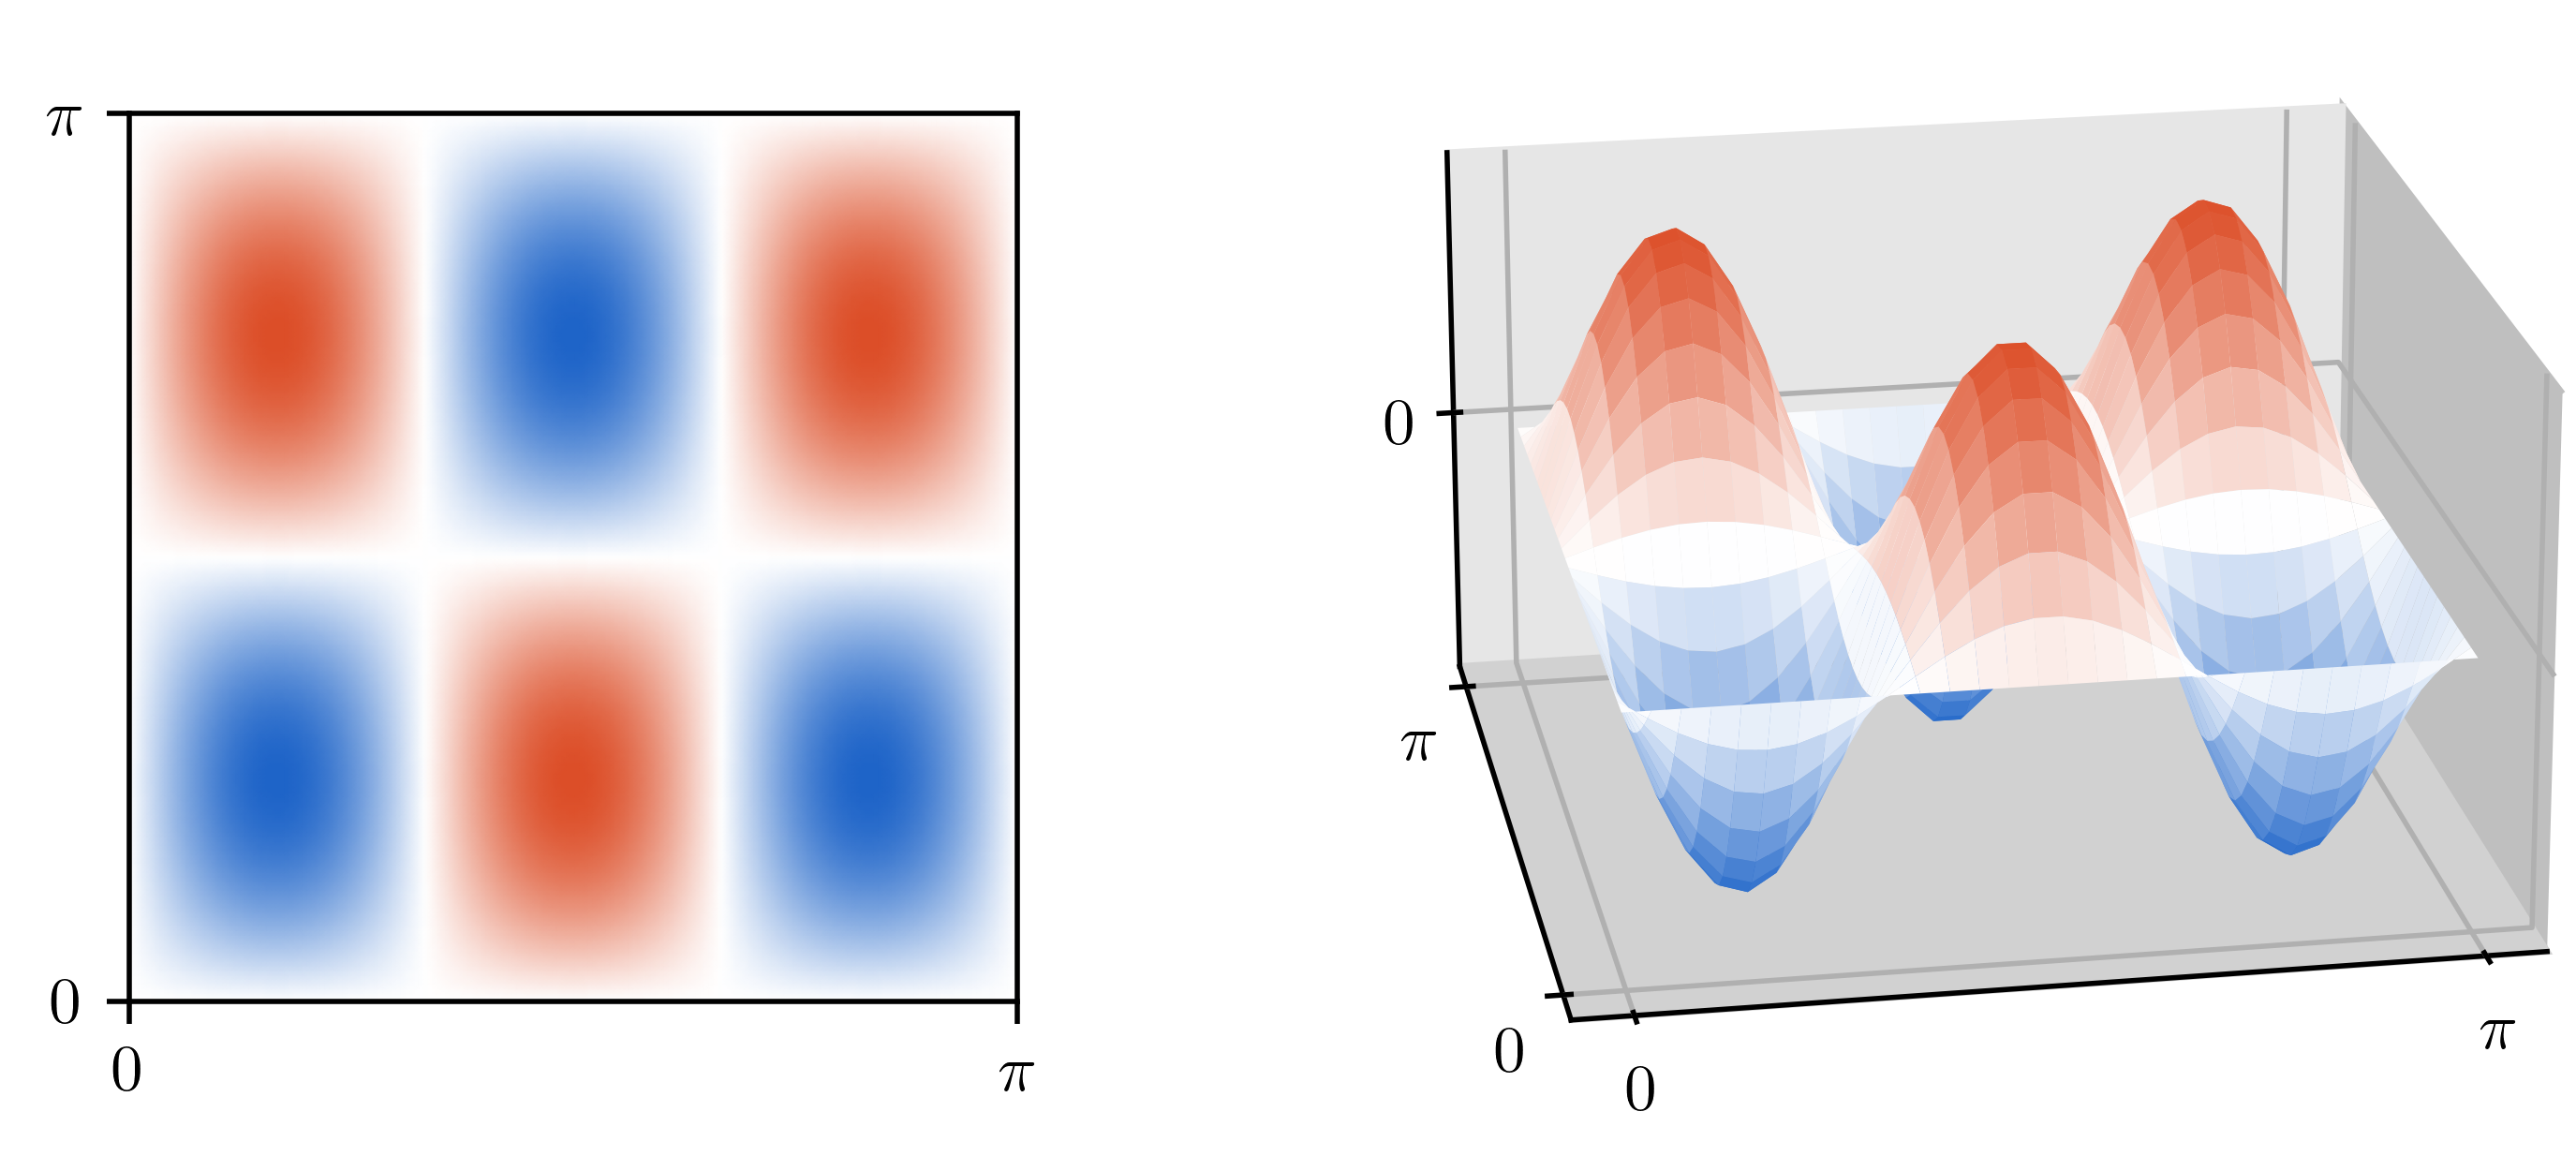
\includegraphics[width=\textwidth]{img/chapter3/example_zero_both.png}
  \end{center}
  \caption{A 2D and 3D plot of the eigenfunction corresponding to $i = 3$ and $j = 2$ from equation~\eqref{equ:c3_zero_example_eigenfunctions}, the eigenvalue is $E_{3,2} = 13$.}\label{fig:example_zero}
\end{figure}

As an example we consider the Schrödinger problem on the domain $[0, \pi] \times [0, \pi]$ with homogeneous Dirichlet boundary conditions and zero potential. Its equation is given as
\begin{equation}\label{equ:c3_example_zero_potential}
  -\pdv[2]{\psi}{x} - \pdv[2]{\psi}{y} = E \psi(x, y)\text{.}
\end{equation}

Now we write an eigenfunction $\psi(x, y)$ as a $y$-dependent linear combination of the $x$-dependent functions $\sin(x)$, $\sin(2x)$, $\sin(3x)$, $\dots$ which satisfy the boundary conditions:
\begin{equation}\label{equ:c3_zero_example_sin_basis}
  \psi(x, y) = \sum_{i=1}^\infty c_i(y) \sin(ix)\text{.}
\end{equation}

Since $\{\sin(x), \sin(2x), \dots\}$ constructs a basis for $L^2_0(\Omega)$, this is the space of compactly supported square integrable functions on $\Omega$, all possible eigenfunctions are expressed with equation~\eqref{equ:c3_zero_example_sin_basis}. If we plug this into the Schrödinger equation then we get
$$
  \sum_{i=1}^\infty i^2 c_i(y) \sin(ix) - \sum_{i=1}^\infty \dv[2]{c_i}{y}(y) \sin(ix) = \sum_{i=1}^\infty E c_i(y) \sin(ix)\text{.}
$$
Linear combinations of basis functions can only be equal if their coefficients are equal, thus:
\begin{equation}\label{equ:c3_zero_example_ode}
  (i^2 - E) c_i(y) = \dv[2]{c_i}{y}(y) \quad \text{ with $c_i(0) = c_i(\pi) = 0$ for each $i \in \{1, 2, \dots\}$.}
\end{equation}
Define $j := \sqrt{E - i^2}$. The ordinary differential equation~\eqref{equ:c3_zero_example_ode} will only have solutions that satisfy the given boundary conditions if $j$ is a strictly positive integer, specifically: $c_i(y) = \sin\left(\sqrt{E-i^2} y\right)$. This implies that all eigenvalues of~\eqref{equ:c3_example_zero_potential} are
$$
  E_{i, j} = i^2 + j^2 \quad \text{ for all $i, j \in \{1, 2, \dots\}$}
$$
with corresponding eigenfunction
\begin{equation}\label{equ:c3_zero_example_eigenfunctions}
  \psi_{i,j} = \sin(ix) \sin(jy)\text{.}
\end{equation}

The eigenvalues are summarized in the following table.

\begin{tabular}{ccccccc}
  \toprule
  $0$       & $1$,$2$             & $3$       & $4$,$5$             & \dots & $30$, $31$, $32$              & \dots \\
  \midrule
  $E_{1,1}$ & $E_{1,2} = E_{2,1}$ & $E_{2,2}$ & $E_{1,3} = E_{3,1}$ & \dots & $E_{1,7} = E_{5,5} = E_{7,1}$ & \dots \\
  $2$       & $5$                 & $8$       & $10$                & \dots & $50$                          & \dots \\
  \bottomrule
\end{tabular}

Here we see that there are many degenerate eigenvalues, the $30^\text{th}$ eigenvalue $50$ even has multiplicity three. The $234^\text{th}$ eigenvalue with value $325$ even has multiplicity six. With some number theory, one can prove that the multiplicity of an eigenvalue can be unbounded.

A visualization of the eigenfunctions is found in figure~\ref{fig:example_zero}. Here we have visualized the surface in a three-dimensional plot on the right. For clarity, we will use most of the time the two-dimensional representation on the left. Note that no color-legend is provided in the two-dimensional representation, as eigenfunctions may always be scaled.

The eigenvalue corresponding to the eigenfunction from figure~\ref{fig:example_zero} has multiplicity two. Another linear independent eigenfunction can be found by swapping $x$ and $y$.

For almost all potential functions $V$ however, the corresponding Schrödinger equation cannot be solved symbolically. So when one is interested in solutions, one has to resort to numerical methods. When only the ground state, that is the lowest eigenvalue, or maybe only few of the lowest eigenvalues are required, general numerical methods may suffice. Some examples of such techniques are finite difference based methods, or a finite element analysis. When higher eigenvalues are required, the eigenfunctions become more and more oscillatory. For the one-dimensional problem we have seen that general methods have difficulties with highly oscillatory functions. These same difficulties are expected for two-dimensional problems. In chapter~\ref{cha:c4}, we will study such a more general method, and develop our own method.

This chapter is dedicated to the study and improvement of the method proposed in~\cite{ixaru_new_2010} by Ixaru. In section~\ref{sec:c3_ixarus_method}, we will follow~\cite{ixaru_new_2010} and study the method itself. Later on, in section~\ref{sec:c3_improvements} we will highlight some challenges with using this method, and propose some improvements. Section~\ref{sec:c3_index_of_e} contains the new theory we have developed to determine the index of an eigenfunction. And lastly, in section~\ref{sec:c3_experiments} some numerical experiments are presented.

\section{Ixaru's method}\label{sec:c3_ixarus_method}

The main idea of Ixaru's method is built on the well-established technique (by, among others, Titchmarsh~\cite{titchmarsh_eigenfunction_1962}) of writing a solution as a linear combination of well-chosen one-dimensional basis functions $b_i(x)$: $\psi(x, y) = \sum_{i=1}^\infty b_i(x) c_i(y)$. A disadvantage of this known technique is that many basis functions are necessary to represent an eigenfunction accurately along the whole of the domain. Ixaru mitigates this by proposing multiple sets of basis functions, depending on the position in the domain. More concretely, he suggests splitting the domain into $K$ different sectors along the $y$-axis\footnote{In the original article~\cite{ixaru_new_2010}, the domain is split along the $x$-axis. But for notational purposes, it is more convenient to split along the $y$-axis. Analogous for the 3d version of the method, the split would happen along the $z$-axis.}:
$$
  \ymin = y_0 < y_1 < y_2 < \dots < y_k < \dots < y_{K-1} < y_{K} = \ymax\text{.}
$$
This split in sectors is illustrated in figure~\ref{fig:c3_2dsectors}.

\begin{figure}
  \begin{center}
    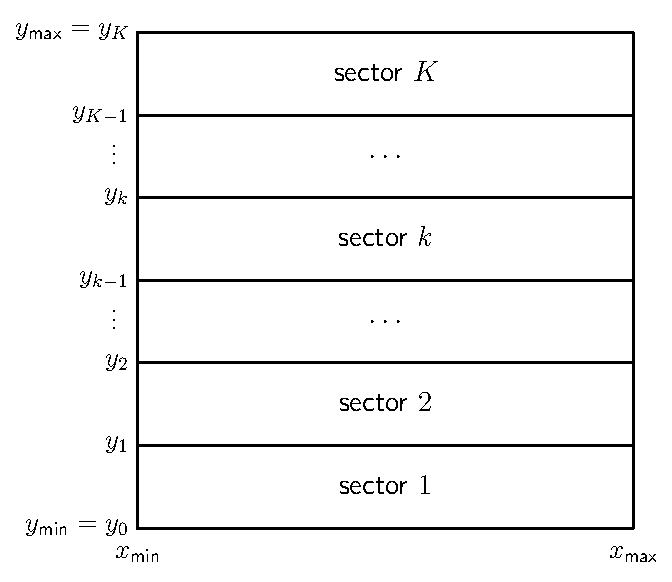
\includegraphics[width=.6\textwidth]{img/chapter3/2dsectors.pdf}
    \caption{\label{fig:c3_2dsectors} An illustration of the split in sectors along the $y$-axis for the domain $[\xmin, \xmax]\times[\ymin, \ymax]$.}
  \end{center}
\end{figure}

On each sector $k$ (with domain $[\xmin, \xmax]\times[y_{k-1}, y_k]$), a solution $\psi(x, y)$ will be approximated as a linear combination of $N$ basis functions:
\begin{equation}\label{equ:c3_lincomb_basis}
  \psi(x, y) \approx \sum_{i=1}^{N} b_i^{(k)}(x) c_i^{(k)}(y) = \transpose{{\vb{b}^{(k)}}}(x) \, \vb{c}^{(k)}(y) \text{.}
\end{equation}

Ideally, the used basis on sector $k$ should be related to the resulting eigenfunction on this sector. Of course, the eigenfunction is unknown, so using it is not an option. In principle, there are many bases to choose from, a Fourier-basis is possible, or some basis based upon orthogonal polynomials. But, these well-known choices do not take advantage of the shape of the potential in the sector. In~\cite{ixaru_new_2010}, the author proposes to use the eigenfunctions from the following one-dimensional Schrödinger problem:
\begin{equation}\label{equ:c3_one_dimensional_schrodinger}
  -\pdv[2]{b_i^{(k)}}{x} + \bar{V}^{(k)}(x)b_i^{(k)}(x) = \lambda_i^{(k)} b_i^{(k)}(x)
\end{equation}
with boundary conditions $b_i^{(k)}(\xmin) = b_i^{(k)}(\xmax) = 0$. The function $\bar{V}^{(k)}(x)$ is a constant (in the $y$-direction) approximation of the potential $V$ on the $k^\text{th}$ sector.

Using this basis is extremely promising. The basis functions are oscillatory for regions where $\bar{V}$ is small, and have an exponential behavior when $\bar{V}$ is large. This same behavior is expected for the two-dimensional eigenfunctions as well. For a potential function which becomes large, the two-dimensional eigenfunction is expected to be most present in the regions where $V(x, y)$ is small. The chosen one-dimensional basis functions $b_i^{(k)}(x)$ express this same behavior.

In~\cite{ixaru_new_2010}, $\bar{V}^{(k)}(x) := V\left(x, \frac{y_{k-1} + y_k}{2}\right)$ is used as the potential of the one-dimen\-sional problem on sector $k$. We will use this as well, for now. Later, we will remark that in some cases other choices may be beneficial.

Just like the constant perturbation methods for one-dimensional problems, this method employs shooting to locate the eigenvalues. To do so, for a fixed value of $E$, formulae are needed to propagate solutions from the bottom of the domain (along $y = \ymin$) upwards, and from the top of the domain ($y = \ymax$) downwards. So, given a solution at the beginning of sector $k$ expressed in the basis $b_i^{(k)}$: $ \psi(x, y_{k-1}) = \sum_{i=1}^{N} b_i^{(k)}(x)\, c_i^{(k)}(y_{k-1}) $, an expression is constructed to compute $c^{(k)}_i(y_k)$ at the end of the sector. Substituting~\eqref{equ:c3_lincomb_basis} into~\eqref{equ:c3_schrodinger_2d} using~\eqref{equ:c3_one_dimensional_schrodinger} gives rise to
\begin{equation}\label{equ:c3_coupled_system}
  -\pdv[2]{\vb{c}^{(k)}}{y} + \vb{V}^{(k)}(y) \vb{c}^{(k)}(y) = E \vb{c}^{(k)}(y) \text{.}
\end{equation}

In this expression $\vb{V}^{(k)}$ is an $N\times N$ matrix depending on $y$:
\begin{equation}\label{equ:c3_v_matrix}
  \vb{V}^{(k)}_{ij}(y) = \int_{\xmin}^{\xmax} b_i^{(k)}(x) b_j^{(k)}(x) \left(V(x, y) - \bar{V}^{(k)}(x)\right) \dd x + \delta_{ij} \lambda_i^{(k)} \text{.}
\end{equation}

The system of ordinary differential equations given in~\eqref{equ:c3_coupled_system} is a coupled system of Schrö\-dinger equations. For coupled systems, there are implementations of constant perturbation methods available, \lilix{}~\cite{ixaru_lilix_2002} or \matscs{}~\cite{ledoux_numerical_2007} for example.

For the accurate computation of the integral in~\eqref{equ:c3_v_matrix} we have developed specialized formulae. These will be presented later on in section~\ref{sec:c3_calculate_vk}.

To be able to propagate a solution along the whole domain, it is vital to have an expression to transfer solutions between consecutive sectors. Eigenfunctions should be continuous and continuously differentiable. To ensure this when transitioning between sectors, we impose for all values $x \in [\xmin, \xmax]$:
\begin{align*}
  \transpose{\vb{b}^{(k)}}(x) \, \vb{c}^{(k)}(y_k)                   & =\, \transpose{\vb{b}^{(k+1)}}(x) \, \vb{c}^{(k+1)}(y_k)                            \\
  \text{and}\quad
  \transpose{\vb{b}^{(k)}}(x)\,\pdv{\vb{c}^{(k)}}{y}\left(y_k\right) & = \transpose{\vb{b}^{(k+1)}}(x)\,\pdv[]{\vb{c}^{(k+1)}}{y}\left(y_k\right) \text{.}
\end{align*}
Multiplying both sides with $\vb{b}^{(k)}(x)$ and integrating along the $x$-axis for each $i \in \{1, \dots, N\}$ yields
\begin{align*}
  \vb{c}^{(k+1)}(y_k)                       & = \vb{M}^{(k)} \vb{c}^{(k)}(y_k)                       \\
  \pdv[]{\vb{c}^{(k+1)}}{y}\left(y_k\right) & = \vb{M}^{(k)} \pdv[]{\vb{c}^{(k)}}{y}\left(y_k\right)
\end{align*}
with
$$
  \vb{M}^{(k)}_{ij} = \bra{b_{i}^{(k)}}\ket{b_{j}^{(k+1)}} = \int_\xmin^\xmax b_i^{(k)}(x) b_j^{(k+1)}(x) \dd x \text{.}
$$
Here we assumed the orthogonal basis $\{b_i^{(k)}(x)\}$ to be normalized $\langle b_{i}^{(k)} | b_{j}^{(k)} \rangle = \delta_{ij}$, or in matrix notation:
\begin{equation}\label{equ:c3_b_orthonormal}
  \int_\xmin^\xmax \transpose{\vb{b}} \vb{b}\,\dd x = \vb{I}\text{.}
\end{equation}

\begin{figure}
  \begin{center}
    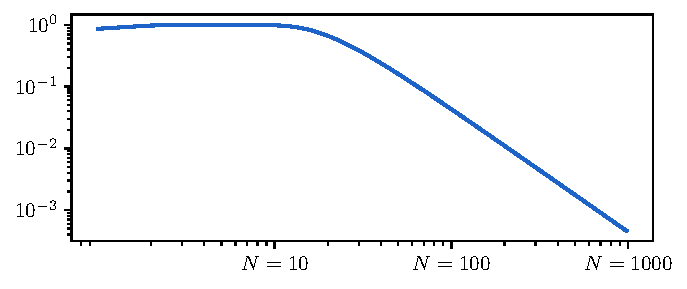
\includegraphics[width=\textwidth]{img/chapter3/orthogonal_m.pdf}
  \end{center}
  \caption{Let $\vb{N}$ be the upper left $N \times N$ block of $\vb{M}$, with $\vb{M}$ the transition between the bases defined by the Schrödinger problems with potentials $V(x) = (x-1)^2$ and $V(x) = (x+1)^2$. This graph displays $\left\| \vb{N} \transpose{\vb{N}} - I \right\|_2$ as a function of $N$.}\label{fig:c3_orthogonal_m}
\end{figure}

Since in the infinite case
\begin{equation}\label{equ:c3_m_before_truncation}
  c^{(k+1)}_i = \sum_{i=0}^{\infty} \bra{b_j^{(k)}}\ket{b_i^{(k+1)}} c^{(k)}_j
\end{equation}
exactly, this matrix $\vb{M}^{(k)}$ is orthogonal. However, if the sum on the right hand-side of~\eqref{equ:c3_m_before_truncation} is truncated, then ${\vb{M}^{(k)}}^\transposesign$ no longer reverses this transformation. Therefore, $\vb{M}^{(k)}$ is in general no longer orthogonal. As an extreme example consider the transition matrix $\vb{M}$ from the basis defined by $-b_i'' + (x-1)^2 b_i = \lambda_i b_i$ to the basis defined by $-b_i'' + (x+1)^2 b_i = \lambda_i b_i$. The infinite matrix $\vb{M}$ is orthogonal, any finite upper left block of $\vb{M}$ is not orthogonal. This is demonstrated in figure~\ref{fig:c3_orthogonal_m}. This loss of orthogonality is a minor inconvenience, inherent to this method.

With these tools available, all that is left is to formalize how the shooting can be executed. Instead of propagating with a single starting condition (i.e. a column vector $\vb{c}^{(1)}(\ymin)$), all possible initial values (for homogeneous Dirichlet boundary conditions) are propagated at once. Therefore, we propose to start with:
$$
  \begin{matrix}
    \vb{C}^{(1)}(\ymin) = \vb{0}_{N\times N} &            & {\pdv[]{}{y}}\vb{C}^{(1)}(\ymin) = \vb{I}_{N\times N}                    \\
                                             & \text{and} &                                                                          \\
    \vb{C}^{(K)}(\ymax) = \vb{0}_{N\times N} &            & {\pdv[]{}{y}}\vb{C}^{(K)}\left(\ymax\right) = \vb{I}_{N\times N}\text{.}
  \end{matrix}
$$

As we are using a multiple shooting procedure in the $y$-direction, the propagated values come together in a matching line $y = y_m$. Since eigenfunctions have to be continuous and continuously differentiable, a `matching' condition can be formulated.  Let us define $\Cbottom$ and $\Cbottom'$ to be the values of $\vb{C}^{(m)}(y_m)$ and ${\pdv[]{}{y}}\vb{C}^{(m)}\left(y_m\right)$ respectively when propagated from the bottom of the domain upwards. Analogous $\Ctop$ and $\Ctop'$ can be defined. Now the value $E$ is an eigenvalue of the original problem if and only if there exist vectors $\ubottom$ and $\utop$ such that
\begin{align}
  \Cbottom \cdot \ubottom                   & = \Ctop \cdot \utop           \nonumber                  \\
  \text{and }\quad \Cbottom' \cdot \ubottom & = \Ctop' \cdot \utop \text{.} \label{ref:c3_c1_matching}
\end{align}
In~\cite{ixaru_new_2010}, $\Cbottom$ and $\Ctop$ are implicitly assumed to be non-singular. With this, equations~\eqref{ref:c3_c1_matching} can be rearranged. This makes it equivalent with saying: $E$ is an eigenvalue of~\eqref{equ:c3_schrodinger_2d} if and only if the mismatch matrix
\begin{equation}\label{equ:c3_psi_e}
  \vb{\Phi}(E) := \Cbottom'\Cbottom^{-1} - \Ctop'\Ctop^{-1}
\end{equation}
has a zero eigenvalue. Each linear independent eigenvector of $\vb{\Phi}(E)$ corresponding to eigenvalue $0$ implies a linear independent eigenfunction $\psi(x, y)$ of the Schrödinger equation. Conversely, each eigenfunction of the Schrödinger equation corresponding to $E$ will emit a singular vector for~\eqref{equ:c3_psi_e}. Therefore, the geometric multiplicity of the zero eigenvalue of this matrix is the same as the multiplicity of $E$ as an eigenvalue of~\eqref{equ:c3_schrodinger_2d}. In the original article no details are provided about how one should find the values of $E$ for which the matrix $\vb{\Phi}(E)$ becomes singular. Later, in section~\ref{sec:c3_locating_e}, we will present our method for finding those values. In section~\ref{sec:c3_index_of_e}, we will go even further and demonstrate a technique which allows to determine the index of the eigenvalue in question.

This concludes our overview of the method described by Ixaru in~\cite{ixaru_new_2010}. There are a few differences between our overview and the method as described in~\cite{ixaru_new_2010}. Most notably, as stated in the beginning, we have swapped the roles of $x$ and $y$. To highlight the recursive nature of this method, we have chosen to apply the split along the $y$-axis. To use this method for three-dimensional problems, we split the domain along the $z$-axis, and for the basis functions on each sector we solve the two-dimensional Schrödinger problem in the $x\,y$-plane. For each of these two-dimensional problems, we split the domain along the $y$-axis and solve some one-dimensional Schrödinger problems along the $x$-axis.

\section{Our improvements}\label{sec:c3_improvements}

The numerical experiment in~\cite{ixaru_new_2010} makes this method seem promising. However, we have identified some possibilities where Ixaru's method can be expanded or improved. This section follows primarily our work from~\cite{baeyens_fast_2020}.

We have made four large improvements and present them here in no particular order. First in section~\ref{sec:c3_improvement_automatic_sectors}, we make the program able to automatically choose the optimal sector size. This automatic sector selection allows for a user to only need to specify the required accuracy of the results. In section~\ref{sec:c3_improvement_orthonormalization}, we construct a formula to compute the inner product of two eigenfunctions. This formula allows us to normalize eigenfunctions and to construct an orthogonal basis of the eigenspace for degenerate eigenvalues. Section~\ref{sec:c3_calculate_vk} is dedicated to the computation of the integral in equation~\eqref{equ:c3_v_matrix}. And the last improvement we present here is a robust way to locate eigenvalues in section~\ref{sec:c3_locating_e}. For this last improvement we have to develop some new theoretical results, which we will cover in section~\ref{sec:c3_index_of_e}.

% Should we say something about scaling in between sectors?
% No, too much work, same idea as in MatSCS

\subsection{Automatic optimal sector size}\label{sec:c3_improvement_automatic_sectors}

When developing numerical methods (for any problem, not only for differential equations), it is most user-friendly to ask a user to only specify to which accuracy results are required. Everything else should be automatic\footnote{For example, an implementation of an adaptive quadrature rule should let the user specify only the function to integrate and the accuracy required. No extra parameters, such as the initial number of grid points or the order of the method for example, should be required. But ideally, a user who is experimenting or wants more control should be able to specify any of these extra parameters.}. In \matslise{3}, we have followed \matslise{2}, which has automatic sector size built in. The usability of this two-dimensional method improves if we include something similar.

The same ideas from \matslise{} can be used here as well. The only minor difference is the way we compute the error for a given sector. In the one-dimensional case, the difference between the $16^\text{th}$ and $18^\text{th}$ order propagation matrix is used to estimate the error. In Ixaru's method we are propagating a coupled system of Schrödinger equations on each sector. This propagation is implemented with an adaptation of \matscs{}~\cite{ledoux_numerical_2007}. In this adaptation, the difference between propagating with a $8^\text{th}$ order and a $10^\text{th}$ order method is used as an error estimate.

In theory and in practice this works beautifully, but some optimizations are still possible. The selection algorithm works by guessing an initial sector size $s_0$. When the error is too large, a smaller sector size $s_1$ is chosen and the process starts over. One big disadvantage of this method is that when a sector was computed with an error that is too large, all computations are thrown away and everything is recomputed. This is quite wasteful when the sector size is only slightly adjusted. One of the things we can reuse are the basis functions. Initially these are computed as the solution of
$$
  -\pdv[2]{b_i}{x} + V(x, \bar{y}) = \lambda_i b_i\text{,}
$$
with $\bar{y} = y_{k} + \frac{s_0}{2}$. But if $\frac{s_1}{2} \approx \frac{s_0}{2}$ then it is maybe not necessary to recompute these basis functions. In our testing, we have seen that the algorithm is not very sensitive to when $\frac{s_1}{2}$ is no longer considered close to $\frac{s_0}{2}$. We have chosen the heuristic that $y_k + \frac{s_1}{3} \leq \bar{y} \leq y_k + \frac{2 s_1}{3}$. Intuitively this means that our program reuses the basis functions $b_i$ as long as the corresponding $\bar{y}$ is situated within the middle third of a sector. Another big advantage of not needing to recompute the basis functions is that the expensive recursive expressions for the integrals $\int_{0}^{h} b_i(\delta)b_j(\delta)\delta^n \dd \delta $ can be reused as well. These expressions will be calculated in section~\ref{sec:c3_calculate_vk}.

\begin{figure}
  \begin{center}
    \begin{minipage}[b]{.59\textwidth}
      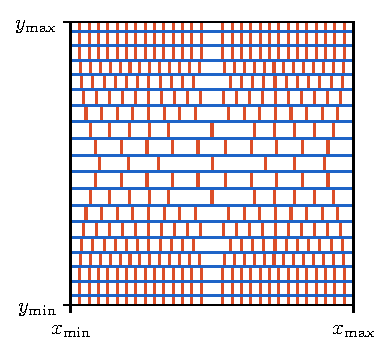
\includegraphics[width=\textwidth]{img/chapter3/sector_example.pdf}
    \end{minipage}
    \hfill
    \begin{minipage}[b]{.4\textwidth}
      \caption{A possible sector selection for problem~\ref{sec:c3_experiment_ixaru} with potential $V(x, y) = (1+x^2)(1+y^2)$. The blue lines indicate sector boundaries. The red lines visualize the piecewise approximation used by \matslise{3} for each of the $x$-directional problems.}\label{fig:c3_sector_selection_example}
    \end{minipage}
  \end{center}
\end{figure}

A possible automatic sector selection is visualized in figure~\ref{fig:c3_sector_selection_example}. Here we have run our implementation on the problem from section~\eqref{sec:c3_experiment_ixaru}. We notice that in the middle of the domain, where the graph of the potential $V(x, y) = (1+x^2)(1+y^2)$ lies lower and is less steep, the sectors are larger.

\subsection{Orthonormalization of eigenfunctions}\label{sec:c3_improvement_orthonormalization}

For the one-dimensional case, we know from theory that eigenfunctions corresponding to different eigenvalues are necessarily orthogonal. In theorem~\ref{the:c3_eigs_othogonal} we have seen that eigenfunctions for different eigenvalues will always be orthogonal. But up to now, nothing has been stated about eigenfunctions corresponding to the same eigenvalue. For degenerate eigenvalues, the eigenspace will be multidimensional.

Ideally, the eigenfunctions returned by our program should form an orthonormal basis. For this we need to normalize eigenfunctions, and ensure that the returned basis of a multidimensional eigenspace is orthogonal. To execute normalization, the inner product $\bra{u}\ket{u} := \int_\Omega u^2$  of an eigenfunction $u$ with itself should be computed. To orthogonalize two linear independent eigenfunctions in the same eigenspace, a Gram--Schmidt process can be used. For this process, there has to be a way to compute the inner product $\bra{u}\ket{v}$ of two functions $u$ and $v$ in this eigenspace.

To normalize an eigenfunction or to orthogonalize eigenfunctions, in both cases the inner product of two functions should be computable. One way would be to numerically estimate this value with some quadrature rules. In principle this is a valid approach, but in practice, this is quite computationally expensive. Therefore in theorem~\ref{the:c3_dot_product}, we construct specialized formulae to compute these inner products.

Calculating the inner product on the whole domain at once is difficult due to the changes in the used basis $\{b_i^{(k)}\}$ for different sectors. To combat this, theorem~\ref{the:c3_dot_product} is formulated with the assumptions that these $b_i^{(k)}(x)$ are constant in the $y$-direction. To compute the inner product of two eigenfunctions on the whole domain, the theorem can be repeatedly applied on each sector. The proof of this theorem follows the same idea used for the normalization of solutions found with a constant perturbation method for one-dimensional Sturm--Liouville problems.

\begin{theorem}\label{the:c3_dot_product}
  Let $\psi_a(x, y)$ and $\psi_b(x, y)$ be two, not necessarily distinct, real eigenfunctions of the Schrödinger operator corresponding to the same eigenvalue $E$. Denote both eigenfunctions as linear combinations of one-dimensional orthonormal basis functions with $b_i(\xmin) = b_i(\xmax) = 0$ (as described in section~\ref{sec:c3_ixarus_method}, on a single sector).
  \begin{align*}
    \psi_a(x, y) = \transpose{\vb{b}(x)} \vb{c_a}(y) = \sum_i b_i(x) c_{a, i}(y) \text{,}\\
    \psi_b(x, y) = \transpose{\vb{b}(x)} \vb{c_b}(y) = \sum_i b_i(x) c_{b, i}(y) \text{.}
  \end{align*}
  On a rectangular domain $[\xmin, \xmax] \times [\ymin, \ymax]$ the inner product of these two functions can be expressed as
  $$
    \bra{\psi_a}\ket{\psi_b} = \int_\xmin^\xmax \int_\ymin^\ymax \psi_a\psi_b \, \dd y \, \dd x = \left. \left(\pdv{\transpose{\vb{c_a}}}{E} \vb{c_b}' - \transpose{\vb{c_b}}\pdv{\vb{c_a}'}{E} \right) \right|_{y=\ymin}^{y=\ymax} \text{,}
  $$
  with $\vb{c_a}' = \dv[]{\vb{c_a}}{y}$ and $\vb{c_b}' = \dv[]{\vb{c_b}}{y}$.
\end{theorem}
\begin{proof}
  By assumption $\psi_a$ and $\psi_b$ are solutions of the Schrödinger equation:
  \begin{align*}
    -\nabla^2 \psi_a + V \psi_a = E \psi_a \\
    -\nabla^2 \psi_b + V \psi_b = E \psi_b \text{.}
  \end{align*}
  Differentiating the first equation with respect to $E$ and multiplying with $\psi_b$ gives
  \begin{align*}
    - \psi_b \nabla^2\pdv{\psi_a}{E} + V(x, y)\pdv{\psi_a}{E} \, \psi_b & = E \pdv{\psi_a}{E}\psi_b + \psi_a\psi_b \text{.} \\
    \intertext{The second equation can be multiplied with $ \pdv[]{\psi_a}{E}$ to result in}
    -\pdv{\psi_a}{E} \nabla^2\psi_b  + V(x, y)\psi_b\,\pdv{\psi_a}{E}   & = E \psi_b\pdv{\psi_a}{E} \text{.}
  \end{align*}
  The difference of these last two expressions can be integrated over the domain $[\xmin, \xmax]\times[\ymin, \ymax]$ to obtain an expression for the inner product $\bra{\psi_a}\ket{\psi_b}$. For brevity of notation, we omit the integration domain, this is assumed to be $[\xmin, \xmax] \times [\ymin, \ymax]$.

  \begin{align*}
    \iint \psi_a\,\psi_b = & \iint\pdv{\psi_a}{E}\nabla^2\psi_b - \iint \psi_b\nabla^2\pdv{\psi_a}{E}                                                                                                                                               \\
    \intertext{The right-hand side can be calculated by applying Green's second identity\footnotemark}\noalign{\footnotetext{Let $f: \Omega \to \RR$ and $g: \Omega \to \RR$ be twice differentiable functions on $\Omega \subseteq \RR^d$. Green's second identity tells us
        $
          \int_\Omega f \nabla^2 g - g \nabla^2 f \dd \Omega = \oint_{\dOmega} \left(f \nabla g - g \nabla f\right) \cdot \dd \vb{n} \text{,}
        $
        with $\vb{n}$ the normal of $\dOmega$.}}
    =                      & \oint \left(\pdv{\psi_a}{E} \nabla \psi_b \cdot \vb{n} -  \psi_b \nabla \pdv{\psi_a}{E} \cdot \vb{n} \right) \text{.}                                                                                                  \\
    \intertext{This can be written explicitly on the integration domain as}
    =                      & \left.\int_{\xmin}^{\xmax} \left(\pdv{\psi_a}{E} \pdv{\psi_b}{y} -  \psi_b \pdv[2]{\psi_a}{E}{y} \right) \dd x \right|_{y=\ymin}^{y=\ymax}                                                                             \\
                           & +\left.\int_{\ymin}^{\ymax} \left(\pdv{\psi_a}{E} \pdv{\psi_b}{x}-  \psi_b \pdv[2]{\psi_a}{E}{x}  \right) \dd y \right|_{x=\xmin}^{x=\xmax} \text{.}                                                                   \\
    \intertext{Taking into account that the eigenfunctions $\psi_a$ and $\psi_b$ are expressed in terms of an orthonormal set of basis functions $\vb{b}(x)$, as in equation~\eqref{equ:c3_b_orthonormal}, we can simplify the expression to}
    =                      & \left. \left(\pdv{\transpose{\vb{c_a}}}{E} \vb{c_b}' - \transpose{\vb{c_b}}\pdv{\vb{c_a}'}{E} \right) \right|_{y=\ymin}^{y=\ymax}                                                                                      \\
                           & +\left.\int_{\ymin}^{\ymax} \left(\transpose{\vb{b}}\pdv{\vb{c_a}}{E} \transpose{\vb{b}'} \vb{c_b} - \transpose{\vb{b}}\vb{c_b} \transpose{\vb{b}'} \pdv{\vb{c_a}}{E}\right)\dd y \right|_{x=\xmin}^{x=\xmax} \text{.}
  \end{align*}
  Since the basis functions satisfy the Dirichlet boundary conditions\footnote{Note that this proof also works if the basis $\vb{b}$ is assumed to satisfy homogeneous Robin boundary conditions.} $\vb{b}(\xmin) = \vb{b}(\xmax) = \vb{0}$ the last term has to be zero, which proves the theorem.
\end{proof}

In this theorem, it is assumed that the basis in which the eigenfunctions are expanded is constant throughout the whole domain. In our case, this basis changes between sectors. Therefore, when computing the inner product of two eigenfunctions on the domain, theorem~\ref{the:c3_dot_product} will have to be repeatedly employed on each sector separately, with $\ymin = y_{k-1}$ and $\ymax = y_k$. Summing these values across all sectors gives the inner product over the whole domain. This value, in turn, can be used to normalize an eigenfunction or orthogonalize different eigenfunctions for the same eigenvalue.

\subsection{Calculation of \texorpdfstring{$\vb{V}^{(k)}(y)$}{Vk(y)}}\label{sec:c3_calculate_vk}

Another improvement we have made can be found in the calculation of the matrix $\vb{V}^{(k)}(y)$ from equation~\eqref{equ:c3_v_matrix}. When one wants to implement the right-hand side of~\eqref{equ:c3_v_matrix} accurately, some considerations have to be made. As the formula consist of an integral with a relatively complicated integrand, we have to consider in which points this integrand is known. Furthermore, evaluating more points is non-trivial.

In~\cite{ixaru_new_2010}, the author points out that not only the values of the basis functions are known but also the values of their derivatives. To use this, ideas from~\cite{kim_quadrature_2002} are combined with the treatment of exponential fitting with two frequencies in~\cite{ixaru_operations_1997}. This yielded a procedure close to \texttt{CENC1} from~\cite{ixaru_exponential_2004}.

In our case, the story is quite different. Because of our improvements to \matslise{}, we can improve accuracy even further. In particular, the computation of $b_i^{(k)}(x)$ is now efficiently possible in arbitrary points. This allows us to use off-the-shelf adaptive quadrature rules, to ensure accuracy. As this was only a first test to approximate $\vb{V}^{(k)}(x)$, we did not use specialized exponentially fitted methods. When profiling our implementation we found that the time to execute these quadrature formulae was almost negligible.

So in practice, there was little need to improve even further, with the more complicated quadrature formulae from~\cite{ixaru_operations_1997,kim_quadrature_2002,conte_modified_2016}. But, as numerical analysts, we were still curious if some more fundamental improvements were possible. After all, the eigenfunctions $b_i^{(k)}(x)$ are approximated piecewise by a truncated series in the step size $\delta$ and the special functions $\eta_{-1}$, $\eta_{0}$, $\dots$ But also, the function $\bar{V}^{(k)}$ is already approximated by a sixteenth degree polynomial. The only `wildcard', so to speak, is the unknown general function $V(x, y)$, for a fixed value of $y$. In the middle of the $k^\text{th}$ sector, this function is approximated piecewisely. As such, it is reasonable to assume that a piecewise sixteenth degree polynomial can also be accurately fitted on this function $V(x, y)$, if the same grid as for $\bar{V}^{(k)}$ is used.

More formal, let us split the interval $[\xmin, \xmax]$ into the same partition that \matslise{3} used for the piecewise approximation $\xmin = x_0, x_1, \dots, x_K = \xmax$. For a fixed value of $y$ on the section $[x_{l-1}, x_l]$, the potential $V(x, y)$ can be approximated by a sixteenth order polynomial, just like $\bar{V}^{(k)}(x)$. We thus approximate $V(x, y) - \bar{V}^{(k)}(x)$ on $[x_{l-1}, x_l]$ by a polynomial $q_l(x)$. This means that to compute~\eqref{equ:c3_v_matrix}, it is sufficient to be able to evaluate
\begin{equation}\label{equ:vk_quad_sector1d}
  \int_{0}^{h} b_i^{(k)}(x_{l-1}+\delta)b_j^{(k)}(x_{l-1}+\delta)\delta^n\dd \delta
\end{equation}
with $h := x_l-x_{l-1}$.

In chapter~\ref{cha:c2}, we have provided expressions for $b_i^{(k)}(x_{l-1}+\delta)$ as a function of $\delta$ and $Z_i := \delta^2\left(\bar{V}^{(k)}_{l,0}- \lambda^{(k)}_i\right)$:
$$
  b_i^{(k)}(x_{l-1}+\delta) = \sum_{m=-1} c_m(\delta) \eta_m(Z_i)\text{.}
$$
In this expression, $c_m(\delta)$ are known polynomials in $\delta$.

Thus, to reconstruct the value of~\eqref{equ:vk_quad_sector1d}, it is sufficient to compute the value of
\begin{equation}\label{equ:c3_eta_eta_inegral}
  I_{k,l}^n := \int_0^h \eta_k(Z_i) \eta_l(Z_j) \delta^n \dd \delta
\end{equation}
for all appropriate $k$, $l$ and $n$. In the next section, we will develop recursive formulae for this expression.

\subsubsection{Weighted integral of product of two \texorpdfstring{$\eta$}{eta}-functions}

Here, the goal is to develop an expression to compute~\eqref{equ:c3_eta_eta_inegral}. Due to the recursive property of $\eta$-functions
$$
  \eta_k(Z) = \frac{1}{Z}\left(\eta_{k-2}(Z) - (2k-1)\eta_{k-1}(Z)  \right)\text{,}
$$
if the first values of~\eqref{equ:c3_eta_eta_inegral} are known for all $n$, the others follow. So we calculate four integrals symbolically (denote $\theta_i := \bar{V}_0^{(m)} -  \lambda_i$ and $\hat{Z}_i = h^2\theta_i$):
\begin{align*}
  F^0 := I_{-1,-1}^0 & = \frac{h}{\theta_i - \theta_j}\left(\theta_i \eta_0(\hat{Z}_i)\eta_{-1}(\hat{Z}_j) - \theta_j \eta_{-1}(\hat{Z}_i)\eta_0(\hat{Z}_j)\right) \text{,}  \\
  G^0 := I_{-1, 0}^1 & = \frac{-1}{\theta_i - \theta_j}\left(\eta_{-1}(\hat{Z}_i)\eta_{-1}(\hat{Z}_j) - \hat{Z}_i \eta_{0}(\hat{Z}_i)\eta_{0}(\hat{Z}_j)  - 1\right) \text{,} \\
  H^0 := I_{0, -1}^1 & = \frac{1}{\theta_i - \theta_j}\left(\eta_{-1}(\hat{Z}_i)\eta_{-1}(\hat{Z}_j) - \hat{Z}_j \eta_{0}(\hat{Z}_i)\eta_{0}(\hat{Z}_j)  - 1\right) \text{,}  \\
  J^0 := I_{0,0}^{2} & = \frac{h}{\theta_i - \theta_j}\left(\eta_{-1}(\hat{Z}_i)\eta_{0}(\hat{Z}_j) - \eta_{0}(\hat{Z}_i)\eta_{-1}(\hat{Z}_j)\right) \text{.}
\end{align*}
In the case where $i = j$, these values are given as
\begin{align*}
  F^0 := I_{-1,-1}^0 & = \frac{h}{2} \left(\eta_{-1}(\hat{Z}_i) \eta_{0}(\hat{Z}_i) + 1\right) \text{,}            \\
  G^0 := I_{-1, 0}^1 & = \frac{h^2}{2 \hat{Z}_i} \left(\eta_{-1}(\hat{Z}_i)^2 - 1\right) \text{,}                  \\
  H^0 := I_{0, -1}^1 & = G^0 \text{,}                                                                              \\
  J^0 := I_{0,0}^{2} & = \frac{h^3}{2 \hat{Z}_i} \left(\eta_{-1}(\hat{Z}_i) \eta_{0}(\hat{Z}_i) - 1\right) \text{.}
\end{align*}


We next show that it is possible, by partial integration, to compute formulae for $F^{n}:=I_{-1,-1}^{n}$ and $J^{n}:=I_{0,0}^{n+2}$ using values for $G^{n-1}:=I_{-1,0}^{n}$ and $H^{n-1}:=I_{0,-1}^{n}$. Analogous, formulae for $G^{n}$ and $H^{n}$ use the values of $F^{n-1}$ and $J^{n-1}$. Let us consider the case of $F^{n}$. Differentiating both sides of
$$
  \int^{h}_0 \eta_{-1}(Z_i)\eta_{-1}(Z_j)\dd \delta = \frac{h}{\theta_i - \theta_j}\left(\theta_i \eta_0(\hat{Z}_i)\eta_{-1}(\hat{Z}_j) - \theta_j \eta_{-1}(\hat{Z}_i)\eta_0(\hat{Z}_j)\right)\text{,}
$$
with respect to $h$, and replacing $h$ by $\delta$, gives:
$$
  \eta_{-1}(Z_i)\eta_{-1}(Z_j) = \pdv[]{}{\delta}\left(\frac{\delta}{\theta_i - \theta_j}\left(\theta_i \eta_0(Z_i)\eta_{-1}(Z_j) - \theta_j \eta_{-1}(Z_i)\eta_0(Z_j)\right)\right) \text{.}
$$
Then, the partial integration formula
$$
  \int_{0}^h f'(\delta)g(\delta) \dd \delta = f(h)g(h) - f(0)g(0) - \int_0^{h} f(\delta) g'(\delta) \dd \delta
$$
is applied to $g(\delta) = \delta^{n}$ and $f'(\delta) = \eta_{-1}(Z_i)\eta_{-1}(Z_j)$. Since
$$
  f(\delta) = \frac{\delta}{\theta_i - \theta_j}\left(\theta_i \eta_0(Z_i)\eta_{-1}(Z_j) - \theta_j \eta_{-1}(Z_i)\eta_0(Z_j)\right)\text{,}
$$
we obtain
\begin{align*}
  F^{n} & = \int_{0}^{h}\eta_{-1}(Z_i)\eta_{-1}(Z_j) \delta^{n} \dd \delta                                                                                    \\
        & =h^{n} F^0 - \frac{n}{\theta_i - \theta_j}\int_{0}^{h} \delta^{n} \left( \theta_i \eta_{0}(Z_i)\eta_{-1}(Z_j)
  % \right. \\  &\hspace{54mm} \left.
  - \theta_j \eta_{-1}(Z_i)\eta_{0}(Z_j) \right) \dd \delta                                                                                                   \\
        & =h^{n} F^0 - \frac{n}{\theta_i-\theta_j}\left(\theta_i H^{n-1} - \theta_j G^{n-1}\right)\text{.}                                                   \\
  \intertext{With similar computations we obtain the following formulae}
  G^{n} & = \int_{0}^{h}\eta_{-1}(Z_i)\eta_{0}(Z_j) \delta^{n+1} \dd \delta                                                                                   \\
        & = h^{n} G^0 + \frac{n}{\theta_i - \theta_j}\int_0^h \delta^{n-1} \left( \eta_{-1}(Z_i)\eta_{-1}(Z_j)
  %		\right.             \\               %    & \hspace{54mm} \left.
  - \theta_i\delta^2 \eta_{0}(Z_i)\eta_{0}(Z_j)  - 1 \right) \dd \delta                                                                                       \\
        & = h^{n} G^0 + \frac{n}{\theta_i - \theta_j}\left( F^{n-1} - \theta_i J^{n-1}\right) - \frac{h^{n}}{\theta_i - \theta_j}                             \\
  H^{n} & = h^{n} H^0 - \frac{n }{\theta_i - \theta_j}\left( F^{n-1} - \theta_j J^{n-1}\right) + \frac{h^{n}}{\theta_i - \theta_j}                            \\
  J^{n} & = \int_{0}^{h}\eta_{0}(Z_i)\eta_{0}(Z_j) \delta^{n+2} \dd \delta                                                                                    \\
        & = h^{n} J^0 - \frac{n }{\theta_i - \theta_j}\int_0^h \delta^{n} \left( \eta_{-1}(Z_i)\eta_{0}(Z_j) - \eta_{0}(Z_i)\eta_{-1}(Z_j) \right) \dd \delta \\
        & = h^{n} J^0 - \frac{n }{\theta_i - \theta_j}\left( G^{n-1} - H^{n-1} \right)\text{.}
\end{align*}

Calculating these values for increasing $n$ can be a numerically unstable process. A more stable algorithm is made by reversing the recursion with decreasing values of $n$. This gives rise to the recursion:
\begin{align*}
  F^{n-1} & = \frac{1}{n}\left( x_1 \theta_i + x_2 \theta_j + h^n \right) \\
  J^{n-1} & = \frac{1}{n}\left( x_1  + x_2\right)                         \\
  G^{n-1} & = \frac{1}{n}\left( y_1  + \theta_i y_2\right)                \\
  H_{n-1} & = \frac{1}{n}\left( y_1  + \theta_j y_2\right)
\end{align*}
with:
\begin{align*}
  x_1 & = H^{0} h^n - H^n             \\
  x_2 & = G^0 h^n - G^n               \\
  y_1 & = F^{0} h^n - F^{n}           \\
  y_2 & = J^{0} h^n - J^{n}  \text{.}
\end{align*}

In practice, we have found reliable convergence when starting this recursion with $n$ sufficiently large and $F^n$, $G^n$, $H^n$ and $J^n$ replaced by $0$.

%This next section should show that $F^{n} \to 0$ if $n \to \infty$, I don't see how. Alternatively, maybe a Taylor-series?
% Then this recursion can be executed starting with $n$ sufficiently large and with $F^n$, $G^n$, $H^n$ and $J^n$ replaced by $0$. To show this, let us focus on the computation of the $F$ and $J$ integrals (a similar analysis can be made for the $G$ and $H$ integrals).
% One verifies that
% % expressions %for $F^{n-2}$ and $J^{n-2}$, which can be rewritten as
% \begin{align*} F^{n-2} & = \frac {  1 }{n \left( n-1 \right) }
%   \left[ \left( \theta_i+\theta_j \right)\, F^n + 2\,\theta_i\,\theta_j\, J^n \right]                                                                                                       \\
%           & \hspace{7mm} +  \frac{h^{n-1}}{n-1} \left( {\theta_j}\,G^0+\theta_i\,H^0-{\frac {h \left( \theta_i+\theta_j \right) }{n}} F^0-\frac {2\, h \,\theta_i\,\theta_j}{n} J^0 \right) \\
%   \\
%   J^{n-2} & =  \frac {  1 }{n \left( n-1 \right) }
%   \left[ 2\,  F^n + \left( \theta_i+\theta_j\right)\, J^n \right]                                                                                                                           \\
%           & \hspace{7mm} + \frac{h^{n-1}}{n-1} \left( G^0+ H^0-{\frac {2\,h  }{n}} F^0-\frac {h \,\left( \theta_i+\theta_j \right)}{n} J^0 \right)
% \end{align*}
% Repeated application of these formulae shows that % $F^{n-2k}$ can be expressed as the sum of a polynomial in $h$ and 
% \begin{align*}
%   F^{n-2k} & = \frac{(n-2\,k)!}{n!} \left(P^k_F(\theta_i,\theta_j) F^n + P^k_J(\theta_i,\theta_j) J^n \right) + \mathcal{F}^{n-2k}     \\
%   J^{n-2k} & = \frac{(n-2\,k)!}{n!} \left(Q^{k-1}_F(\theta_i,\theta_j) F^n + Q^k_J(\theta_i,\theta_j) J^n \right) + \mathcal{J}^{n-2k}
% \end{align*}
% whereby $P^k_F$, $P^k_J$, $Q^{k}_F$, $Q^k_J$ are polynomials in $\theta_i$ and $\theta_j$ of degree $k$ and whereby $\mathcal{F}^{n-2k}$ and $\mathcal{J}^{n-2k}$ represent terms that depend on $h$, $n$, $\theta_i$,   $\theta_j$ and the values $F^0$, $G^0$, $H^0$ and $J^0$. Since $|F^n|$ and  $|J^n|$ can be bounded by $h^n |F^0|$ and $h^n |J^0|$ respectively, it follows that for sufficiently large values of $n$ and $k$, $F^{n-2k}$ and $J^{n-2k}$ can be accurately approximated by $\mathcal{F}^{n-2k}$ and $\mathcal{J}^{n-2k}$ respectively.

Lastly, the other values for $I_{k,l}^n$, with $k, l > 0$, can be computed via the recursion relation between the $\eta$-functions:
\begin{align*}
  I_{k, l}^n & = \frac{1}{\theta_i} \left(I_{k-2,l}^{n-2} - (2k - 1) I_{k-1,l}^{n-2}\right) \\
  I_{k, l}^n & = \frac{1}{\theta_j} \left(I_{k,l-2}^{n-2} - (2l - 1) I_{k,l-1}^{n-2}\right)\text{.}
\end{align*}

In summary, the formulae developed here can now be used to determine values for~\eqref{equ:c3_eta_eta_inegral}, for all $n$, $k$ and $l$.

\subsubsection{Calculation of \texorpdfstring{$\vb{M}^{(k)}$}{M(k)}}

In the previous section, we have obtained formulae to compute~\eqref{equ:vk_quad_sector1d}. In principle, these formulae could also be extended to compute overlap integrals
$$
  \vb{M}_{ij}^{(k)} = \int_{\xmin}^{\xmax}b_i^{(k)}(x)b_j^{(k+1)}(x)\dd x\text{,}
$$
but there are a few hurdles. First, we would like to use the automatic sector selection algorithm in \matslise{}, as this has the big advantage of ensuring the requested accuracy. Using this automatic sector selection has the consequence of choosing a different partition along the $x$-axis for different sectors in the $y$-direction. However, since $\vb{M}^{(k)}$ requires basis functions on two different sectors, it would be very cumbersome to construct appropriate formulae.

Second, we noted that these recursive expressions for $\vb{V}^{(k)}(y)$ are quite expensive to compute. For $\vb{V}^{(k)}(y)$, this cost can be justified by also reducing function evaluations of the potential $V(x, y)$.

In the case of $\vb{M}^{(k)}$, a similar justification is hard to find because in \matslise{3} it is now possible to evaluate $b^{(k)}_i(x)$ very cheaply in arbitrary points.

For these reasons we have opted to use classical quadrature rules to compute $\int_{\xmin}^{\xmax}b_i^{(k)}(x)b_j^{(k+1)}(x)\dd x$. To ensure sufficiently accurate integration results, the 31-points adaptive Gauss--Kronrod formulae are used. These have a proven track record~\cite{piessens_quadpack_1983}.

% Maybe demonstrate how many $M$ are calculated?


\subsection{Locating eigenvalues}\label{sec:c3_locating_e}

In section~\ref{sec:c3_ixarus_method}, we have studied a method to determine, for a given value $E$, whether it is an eigenvalue. This $E$ will only be an eigenvalue if the matrix from equation~\eqref{equ:c3_psi_e} becomes singular. In~\cite{ixaru_new_2010}, it is suggested to keep track of the smallest (in modulus) eigenvalue of $\Psi(E)$. No information is provided about how one can find such values for $E$.

In the literature, many methods to find roots of functions are available. In introductory textbooks to scientific computing (e.g.~\cite[Chapter~5]{heath_scientific_2002}), the most well-known methods are presented. One of the easiest to implement is the method of interval bisection. In this method the root of a scalar function $f : \RR \to \RR$ is determined by repeatedly halving a search interval. The position of the root can be tracked by ensuring the function $f$ has different signs on the end points of the search interval. This requires that an initial guess for the interval already contains one root. But also, notice that the method will not work when the initial search interval contains two roots, or a root with higher multiplicity for example.

Another well-known technique is Newton's method. Here, the root of a scalar function $f$ can be approximated by iterating the following scheme:
$$
  x_{n+1} = x_n - \frac{f(x_n)}{f'(x_n)}\text{.}
$$
For single roots, this method has a faster rate of convergence. Choosing initial values is also easier, because a value $x_0$ should be chosen only to be `sufficiently close' to a true root. One of the biggest drawbacks of this method is that the derivative of $f(x)$ should be available. For complicated functions, this can be difficult. Extensions of this method exist for which the derivative is not necessary, the secant method for example.

In all these well-known methods, the problem is that they only can be used to find a single root, not all roots. Furthermore, they only work on scalar function $\RR \to \RR$ or vector-functions $\RR^n \to \RR^n$ for which roots are uniquely defined. In our case, we are interested in the situation when any of the eigenvalues of $\eqref{equ:c3_psi_e}$ becomes zero. This does not map directly on any of these classical root-finding algorithms.

To combat these issues with the classical algorithms, we propose a small modification to Newton's method. Suppose an inaccurate approximation $E_0$ of an eigenvalue of the Schrödinger equation~\eqref{equ:c3_schrodinger_2d} is given. Starting from this approximation, we want a fast converging algorithm to find the true eigenvalue $E$. As stated earlier, $E$ is an eigenvalue if and only if it is a value such that the mismatch matrix $\vb{\Phi}(E)$, as defined by~\eqref{equ:c3_psi_e}, is singular.
$$
  \vb{\Phi}(E) := \Cbottom'\Cbottom^{-1} - \Ctop'\Ctop^{-1}\text{.}
$$
In other words, the matrix $\vb{\Phi}(E)$ has to have a zero eigenvalue.

In Newton's method, the derivative of the function in question should be available. Fortunately, in~\cite{ixaru_lilix_2002} and in~\cite{ledoux_cpmp_2006}, procedures are available to compute the derivative of solutions with respect to $E$. In our case, this means that the matrices
$$
  \pdv[]{\Cbottom}{E}, \pdv[]{\Cbottom'}{E}, \pdv[]{\Ctop}{E} \text{ and } \pdv[]{\Ctop'}{E}
$$
are available. This allows us to also compute the derivative of $\vb{\Phi}$ itself. First note, for any invertible matrix $\vb{A}$ that $\left(\vb{A}^{-1}\right)' = -\vb{A}^{-1} \vb{A}' \vb{A}^{-1}$, since $\vb{0} = \left(\vb{A}\vb{A}^{-1}\right)' = \vb{A}' \vb{A}^{-1} + \vb{A} \left(\vb{A}^{-1}\right)'$. It then follows that
\begin{align*}
  \pdv{\vb{\Phi}}{E} = & \left(\pdv{\Cbottom'}{E} - \Cbottom'\Cbottom^{-1}\pdv{\Cbottom}{E}\right) \Cbottom^{-1} \\
                       & - \left(\pdv{\Ctop'}{E} - \Ctop'\Ctop^{-1}\pdv{\Ctop}{E}\right) \Ctop^{-1}\text{.}
\end{align*}

Since we want to find roots within the eigenvalues of $\vb{\Phi}$, it is also valuable to be able to compute the derivative of an eigenvalue with respect to $E$. The derivatives of the eigenvalues of a matrix-function are already known for a long time~\cite{lancaster_eigenvalues_1964}.

\begin{theorem}[Lancaster 1964]\label{the:c3_eigenvalue_derivative}
  Let $\vb{A}(x)$ be a matrix function $\mathbb{C} \to \mathbb{C}^{n\times n}$ such that each coefficient is continuously differentiable with respect to $x$ in the point $x_0$. Furthermore, assume $\vb{A}(x_0)$ to be diagonalizable\footnote{In~\cite{lancaster_eigenvalues_1964}, it is noted that different, less stringent, assumptions may be made on the structure of $\vb{A}(x)$: ``This is equivalent to saying that every eigenvalue of [$\vb{A}(x_0)$] has only linear elementary divisors; or that [$\vb{A}(x_0)$] is diagonable, non-derogatory, non-defective, or similar to a diagonal matrix. This assumption could be replaced by the less restrictive condition that only the eigenvalue [$\lambda$] should have linear elementary divisors.''}.

  Let $\lambda$ be a simple eigenvalue of $\vb{A}(x_0)$ with left and right eigenvectors $\vb{v}$, $\vb{u}$ respectively. It now holds that
  $$
    \left(\dv[]{\lambda}{x}\right)_{x=x_0} = \frac{1}{\transpose{\vb{v}}\vb{u}} \left(\transpose{\vb{v}}\dv[]{\vb{A}}{x} \vb{u} \right)_{x=x_0}\text{,}
  $$
  where $\dv[]{\vb{A}}{x}$ is the matrix with, as coefficients, the derivatives of the corresponding coefficients of $\vb{A}(x)$ with respect to $x$.
\end{theorem}
\begin{proof}
  As $\vb{u}$ and $\vb{v}$ are right, respectively left, eigenvectors corresponding to the eigenvalue $\lambda$, it follows that:
  \begin{equation}\label{equ:c3_eigenvalue_derivative_equ1}
    \transpose{\vb{v}}\vb{A}(x_0)\vb{u}  = \lambda \transpose{\vb{v}}\vb{u}\text{.}
  \end{equation}
  Because all involved variables are dependent on $x$, and we will only take the value (or the value of the derivative) in $x_0$, we will, to ease notation, omit this $x$ dependency and implied evaluation in the point $x_0$. Furthermore, we will denote the derivative with respect to $x$ with a prime ``$'$''. This allows us to write down the derivative of both sides of~\eqref{equ:c3_eigenvalue_derivative_equ1}. These derivatives can further be simplified by using the product rule when applied to matrix multiplications:
  \begin{align*}
    \left(\transpose{\vb{v}}\vb{A}(x_0)\vb{u}\right)'                                                                    & = \left(\lambda \transpose{\vb{v}}\vb{u}\right)'                                                                      \\
    \implies \quad {\transpose{\vb{v}}}'\vb{A}\vb{u} + \transpose{\vb{v}}\vb{A}'\vb{u} + \transpose{\vb{v}}\vb{A}\vb{u}' & = \lambda' \transpose{\vb{v}}\vb{u} + \lambda {\transpose{\vb{v}}}'\vb{u} + \lambda \transpose{\vb{v}}\vb{u}'\text{.}
  \end{align*}
  Using that $\vb{u}$ and $\vb{v}$ are eigenvectors ($\vb{A} \vb{u} = \lambda \vb{u}$ and $\transpose{\vb{v}}\vb{A} = \lambda \transpose{\vb{v}}$), gives us the required expression:
  \begin{align*}
    \transpose{\vb{v}}\vb{A}'\vb{u} & = \lambda' \transpose{\vb{v}}\vb{u}                                         \\
    \implies \quad \lambda'         & = \frac{\transpose{\vb{v}}\vb{A}'\vb{u}}{\transpose{\vb{v}}\vb{u}} \text{.}
  \end{align*}
  Here we assumed $\transpose{\vb{v}}\vb{u} \neq 0$. This concern is addressed in the appendix of~\cite{lancaster_eigenvalues_1964}: by considering the subspaces of left and right eigenvectors corresponding to $\lambda$, it can be proven that $\transpose{\vb{v}}\vb{u}$ never vanishes.
\end{proof}

Some care should be taken when two eigenvalues coincide. In~\cite{lancaster_eigenvalues_1964}, this is handled by considering the left and right eigenvector space corresponding to the multiple eigenvalue. But since we are dealing with only numerical results this (almost) never happens. Theorem~\ref{the:c3_eigenvalue_derivative} applied to $\vb{\Phi}(E)$ gives
$$
  \pdv{\lambda}{E} = \frac{1}{\transpose{\vb{v}}\vb{u}}\transpose{\vb{v}} \pdv{\vb{\Phi}}{E} \vb{u} \text{,}
$$
with left and right eigenvectors $\vb{v}$ and $\vb{u}$ respectively corresponding to the eigenvalue $\lambda$.

With the values for all these derivatives, all tools are available to formulate our proposed modified Newton's scheme. To simplify the notation, we introduce the matrix-operator $\spectrum$ which returns the spectrum of a matrix. This operator is defined on the $n \times n$-matrix $\vb{A}$ as
$$
  \spectrum(\vb{A}) := \left\{\lambda \in \CC \, \middle| \, \exists \vb{u} \in \CC^n \setminus \{\vb{0}\} : \vb{A} \vb{u} = \lambda \vb{u} \right\}\text{.}
$$

\begin{figure}
  \begin{center}
    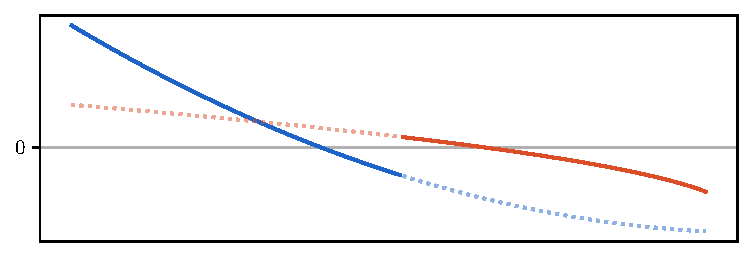
\includegraphics[width=\textwidth]{img/chapter3/select_lambda_newton.pdf}
  \end{center}
  \caption{Two eigenvalues of $\vb{\Phi}(E)$ are plotted. Whichever is preferred by $f(E)$ from~\eqref{equ:c3_mismatch_newton_function} is highlighted.}\label{fig:c3_select_lambda_newton}
\end{figure}

Now, we define the scalar function $f(E) : \RR \to \RR$ as
\begin{equation}\label{equ:c3_mismatch_newton_function}
  f(E) = \argmin_{\lambda \in \spectrum(\vb{\Phi}(E)) \cap \RR} \left|\frac{\lambda}{\pdv*[]{\lambda}{E}}\right|\text{.}
\end{equation}
On this function $f(E)$, the classical Newton's method can be used.

In figure~\ref{fig:c3_select_lambda_newton}, the idea of $f(E)$ from~\eqref{equ:c3_mismatch_newton_function} is demonstrated. Assume the blue line and red line each represents an eigenvalue of $\vb{\Phi}(E)$. The regions where this eigenvalue is chosen by $f(E)$ are indicated. The idea is that $f$ selects the function with the closest possible root in a linear approximation.

\subsubsection{A numerical example}

To provide some intuition about the eigenvalues $\lambda$ of the mismatch matrix $\vb{\Phi}(E)$, we will analyze a numerical example. Consider the two-dimensional time-independent Schrödinger equation with potential function
\begin{equation}\label{equ:c3_mismatch_ixaru}
  V(x, y) = (1+x^2)(1+y^2)
\end{equation}
on the domain $[-5.5; 5.5] \times [-5.5; 5.5]$ with homogeneous Dirichlet boundary conditions. This problem is also the numerical example from Ixaru's work~\cite{ixaru_new_2010}.

\begin{figure}
  \begin{center}
    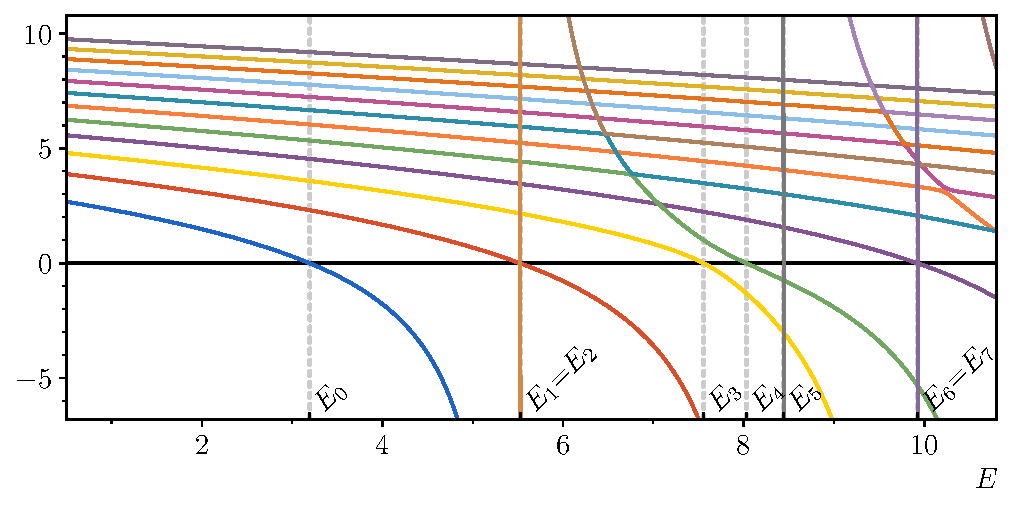
\includegraphics[width=\textwidth]{img/chapter3/mismatch_rainbow.pdf}
  \end{center}
  \caption{Each of the eigenvalues $\lambda$ of the mismatch matrix $\vb{\Phi}(E)$ of the Schrödinger problem~\eqref{equ:c3_mismatch_ixaru} with $N = 12$ as a function of $E$. The true eigenvalues of this problem are indicated with $E_0$, $E_1$, $\dots$ The lines are colored and continued to aid in the clarity of this illustration. But, do notice that this is only a best guess approximation.}\label{fig:c3_mismatch_rainbow}
  \vspace{1cm}
  \begin{center}
    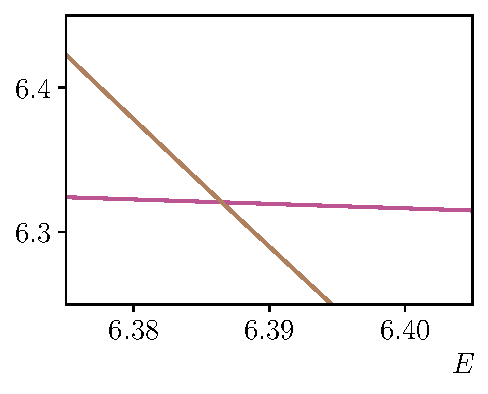
\includegraphics[width=.495\textwidth]{img/chapter3/mismatch_rainbow_zoomed_0.pdf}
    \hfill
    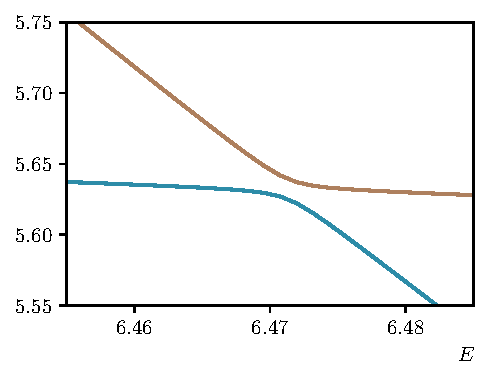
\includegraphics[width=.495\textwidth]{img/chapter3/mismatch_rainbow_zoomed_1.pdf}
  \end{center}
  \caption{These are zoomed in views of the graph from~\ref{fig:c3_mismatch_rainbow}. Some surprising behavior of the eigenvalues of $\vb{\Phi}(E)$ are visible.}\label{fig:c3_mismatch_rainbow_zoom}
\end{figure}

Throughout this research, one of the first graphs we studied can be found in figure~\ref{fig:c3_mismatch_rainbow}. Here all eigenvalues of the mismatch matrix $\vb{\Phi}(E)$ are plotted. For each value of $E$ in this problem, $\vb{\Phi}(E)$ has $N$ real eigenvalues, with $N$ number of functions $b_i^{(k)}(x)$ on each sector, as described in section~\ref{sec:c3_ixarus_method}. Upon seeing this graph, it is easy to say that one can `follow' the trajectory of a single eigenvalue as $E$ changes. In reality, this is not easy at all. For example, sometimes two eigenvalue curves intersect, other times they barely avoid each other, and seemingly switch which curve they follow. In figure~\ref{fig:c3_mismatch_rainbow_zoom}, this strange behavior is visible.


These difficulties and nuances are hidden away behind the colors and seemingly continuous lines present in figure~\ref{fig:c3_mismatch_rainbow}. Practically, this graph is generated from the eigenvalues (and their derivatives) of $\vb{\Phi}(E)$ for $\numprint{10000}$ values of $E$. Two eigenvalues $\lambda^{(i)}_j$, $\lambda^{(i+1)}_k$  for two adjacent values $E_{i}$ and $E_{i+1}$, are determined to correspond to the same curve (and thus get the same color) if
$$ \frac{\lambda^{(i+1)}_k  - \lambda^{(i)}_j}{E_{i+1} - E_i} \approx \dv[]{\lambda^{(i+1)}_k}{E} $$
holds within a given accuracy.

\begin{figure}
  \centering
  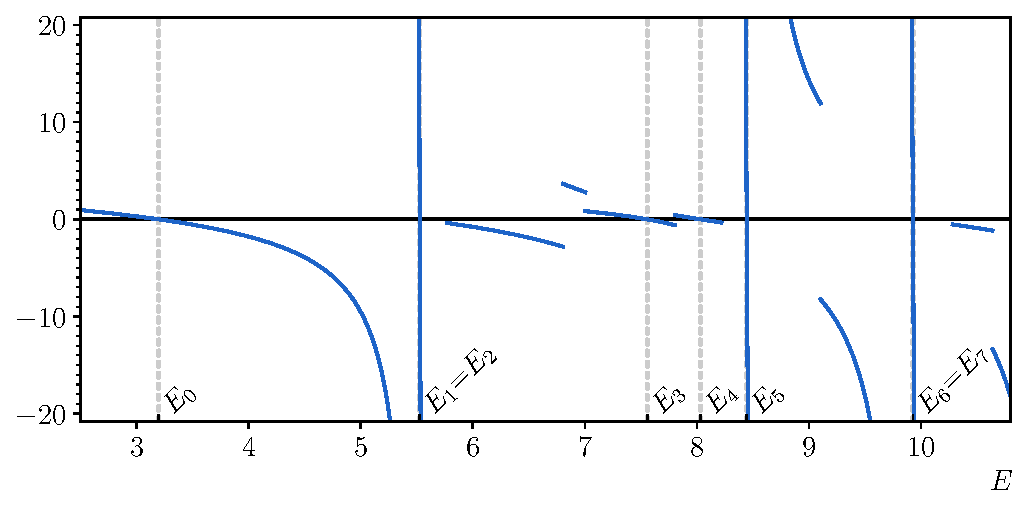
\includegraphics[width=\textwidth]{img/chapter3/mismatch_newton.pdf}
  \caption{The function~\eqref{equ:c3_mismatch_newton_function} for problem~\eqref{equ:c3_mismatch_ixaru} is plotted in blue. In red, we have indicated the smallest real eigenvalue (in absolute value) of $\vb{\Phi}(E)$. In regions where the red curve seems missing, it coincides with the blue curve. At first glance, the striking vertical lines may be assumed to be asymptotes. This is not the case: in these regions, $f(E)$ changes rapidly.}\label{fig:c3_mismatch_newton}
\end{figure}

In figure~\ref{fig:c3_mismatch_newton}, the graph of the function $f(E)$ from equation~\eqref{equ:c3_mismatch_newton_function} is plotted. Comparing this with figure~\ref{fig:c3_mismatch_rainbow}, allows us to get an intuitive understanding of our application of Newton's method. But as can be seen in figure~\ref{fig:c3_mismatch_newton}, this method is not perfect. For example, the region in which eigenvalue $E_5$ can be detected is relatively small. If the more straightforward $f(x) = \argmin_{\lambda \in \spectrum(\vb{\Phi}(E)) \cap \RR} \left|\lambda\right|$ was used, this region would be extremely tiny, as can be seen on figure~\ref{fig:c3_mismatch_newton}. But still, even with~\eqref{equ:c3_mismatch_newton_function}, numerically it would be very unlikely to stumble upon this region, to detect that an eigenvalue was missing. For this reason we have developed a robust way to determine the number of eigenvalues less than the value $E$. This allows us to detect these missing values, and locate them. In the next section (\ref{sec:c3_index_of_e}), we will develop some new theory to locate all eigenvalues reliably.

\section{Determining the index of eigenvalues}\label{sec:c3_index_of_e}

This section is based upon as yet unpublished work, in collaboration with professor Hans Vernaeve.

In mathematical physics there are many problems dependent on, or consisting of, determining eigenvalues of a linear elliptic operator on a given domain with homogeneous Dirichlet boundary conditions. Examples include the Schrödinger equation, the wave equation, and the linear theory of elasticity to name a few. There are many methods, analytical as well as numerical, to solve for or to approximate these eigenvalues, e.g. shooting methods~\cite{ixaru_numerical_1984,ixaru_new_2010}, finite difference methods~\cite{wang_new_2009}, methods for finding the lowest eigenvalues~\cite{braun_efficient_1996}, or even the methods discussed in chapters~\ref{cha:c2},~\ref{cha:c3} and~\ref{cha:c4}. There even exist (numerical) methods that are able to find eigenvalues in the neighborhood of a given value $E$ without the need to compute all lower eigenvalues. For this last group of methods we have developed a theorem to count eigenvalues.

\begin{table}
  \newlength{\hoWidth}
  \setlength{\hoWidth}{.2\linewidth}
  \begin{center}
    \begin{tabular}{rlrl|rl|}
      \multicolumn{2}{|c}{$ \lambda_{0} \approx 2.00$}                                                                     & \multicolumn{2}{|c|}{$ \lambda_{1,2} \approx 4.00 $} & \multicolumn{2}{c|}{$ \lambda_{3,4,5} \approx 6.00 $}                                                                                                                                                                                                                                                             \\ \hline
      \multicolumn{1}{|c}{\parbox[c]{\hoWidth}{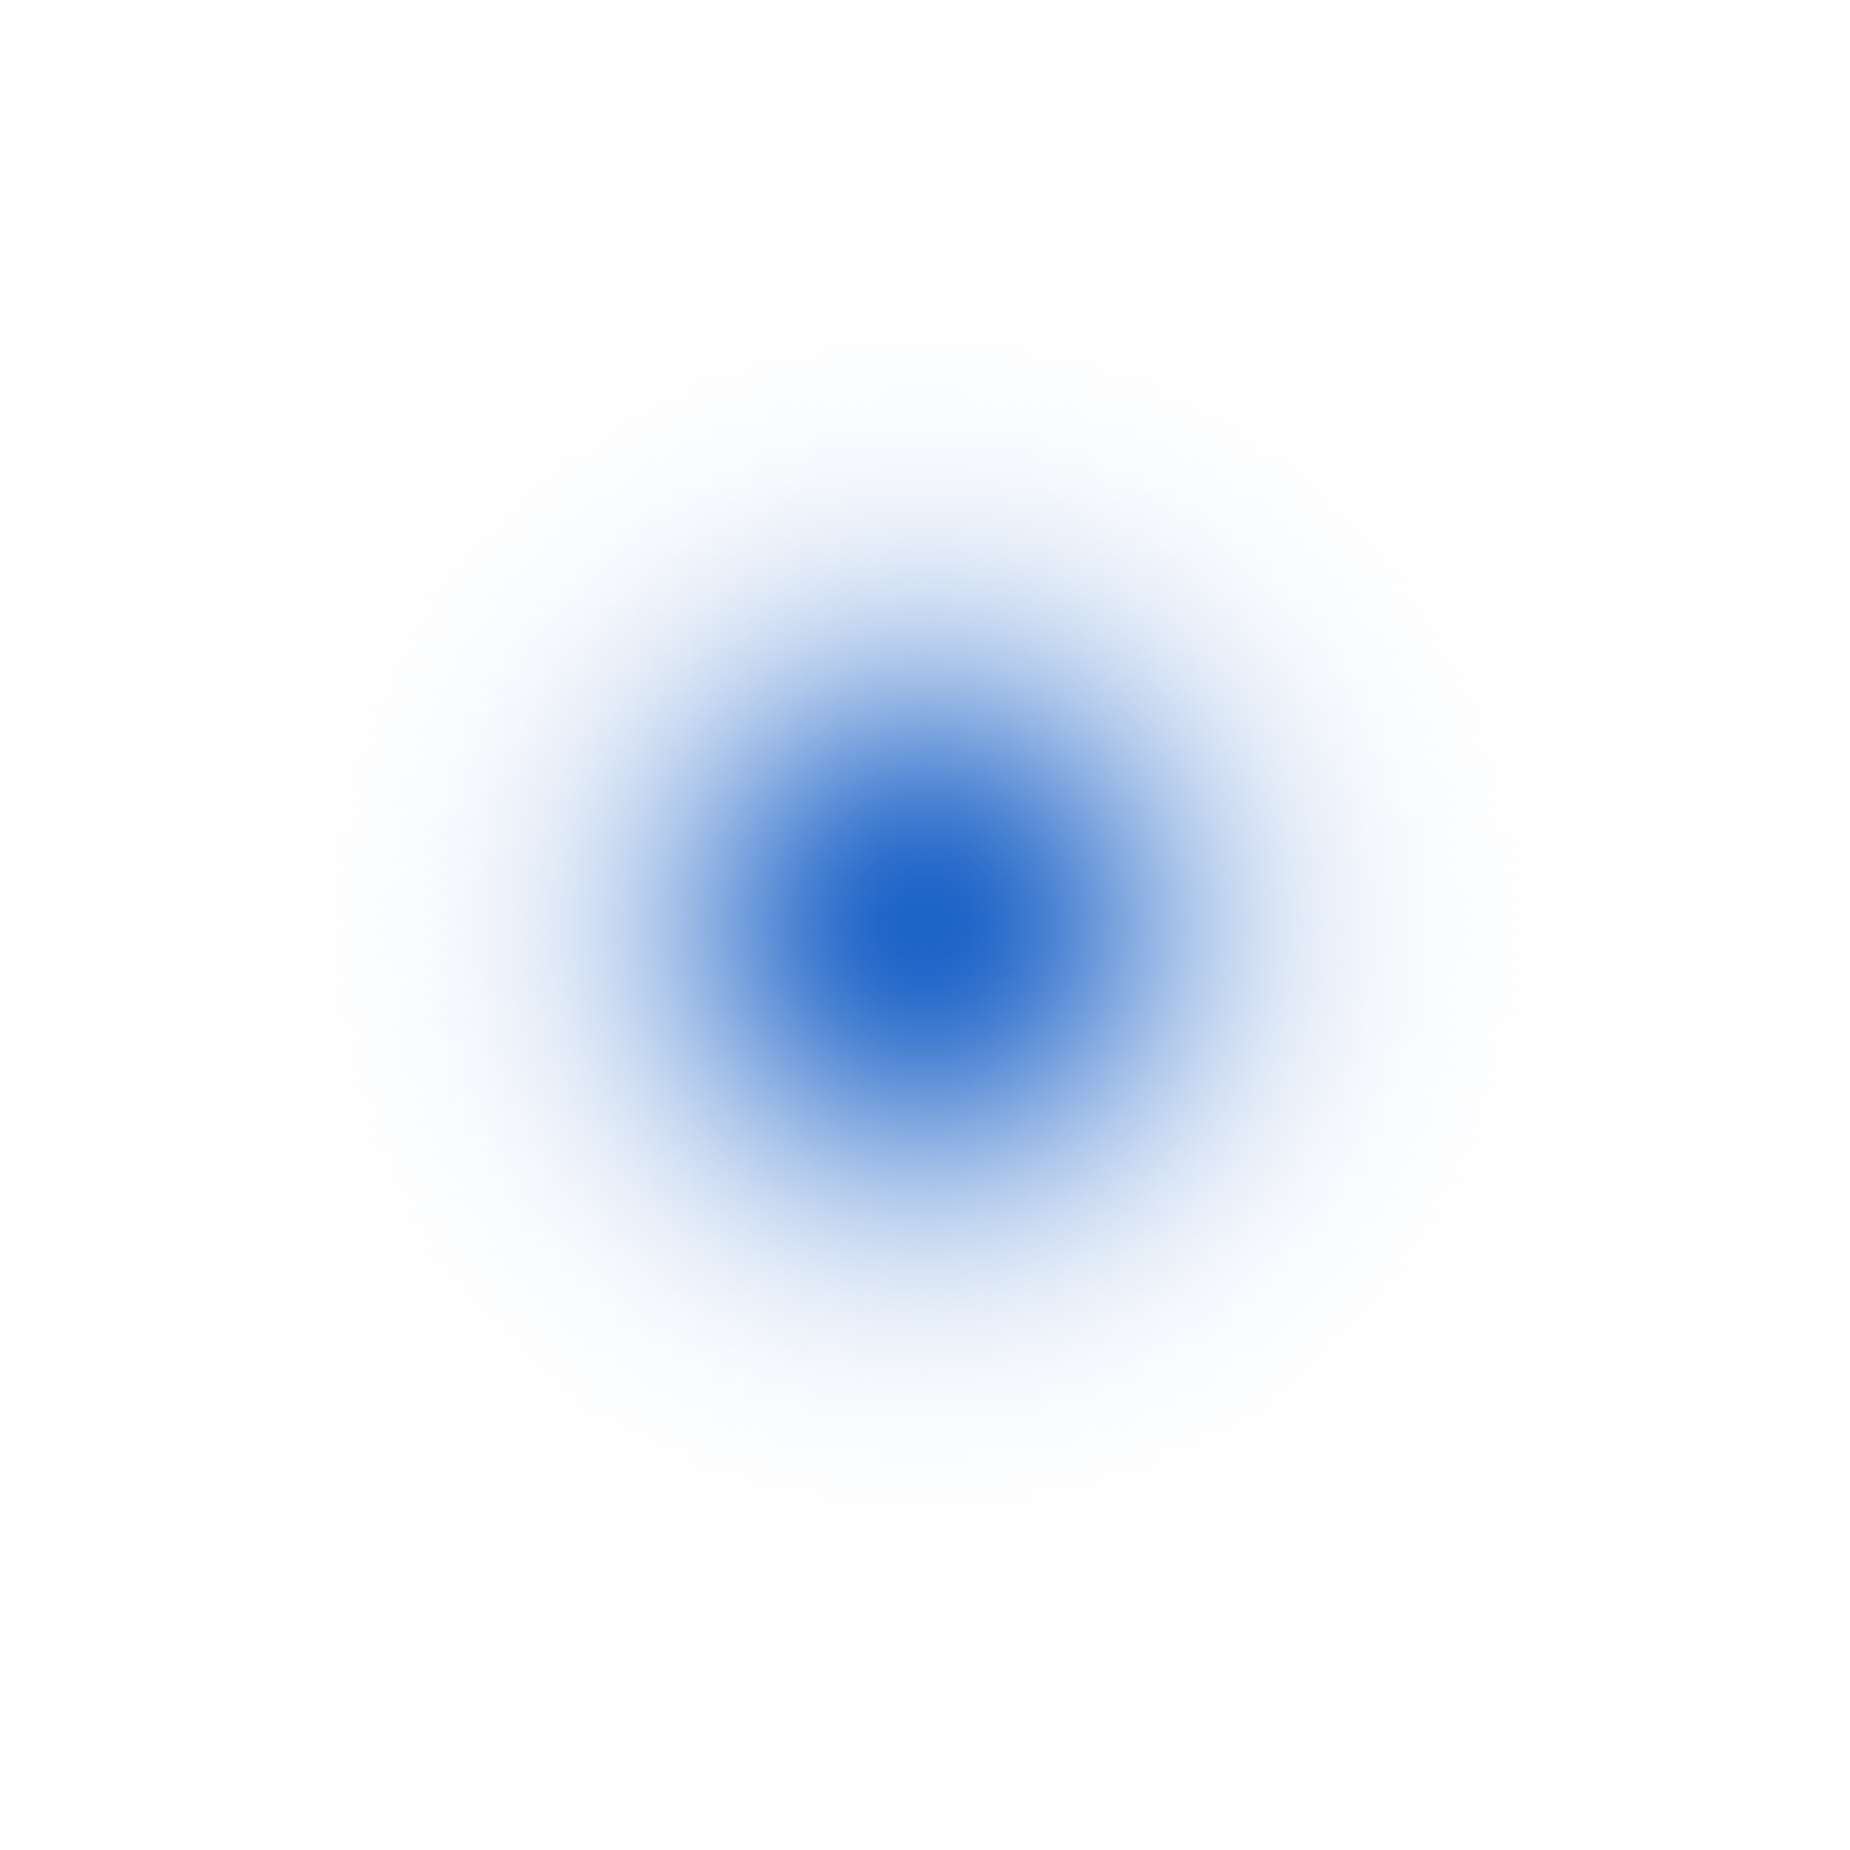
\includegraphics[width=\linewidth]{img/chapter3/counting/harmonic/2a.png}}} & $ \begin{matrix} \mathbf{u_{1,1}} \vspace{5pt}\\ \scalebox{1.5}{$\mathbf{1}$} \end{matrix} $                       & \multicolumn{1}{|c}{\parbox[c]{\hoWidth}{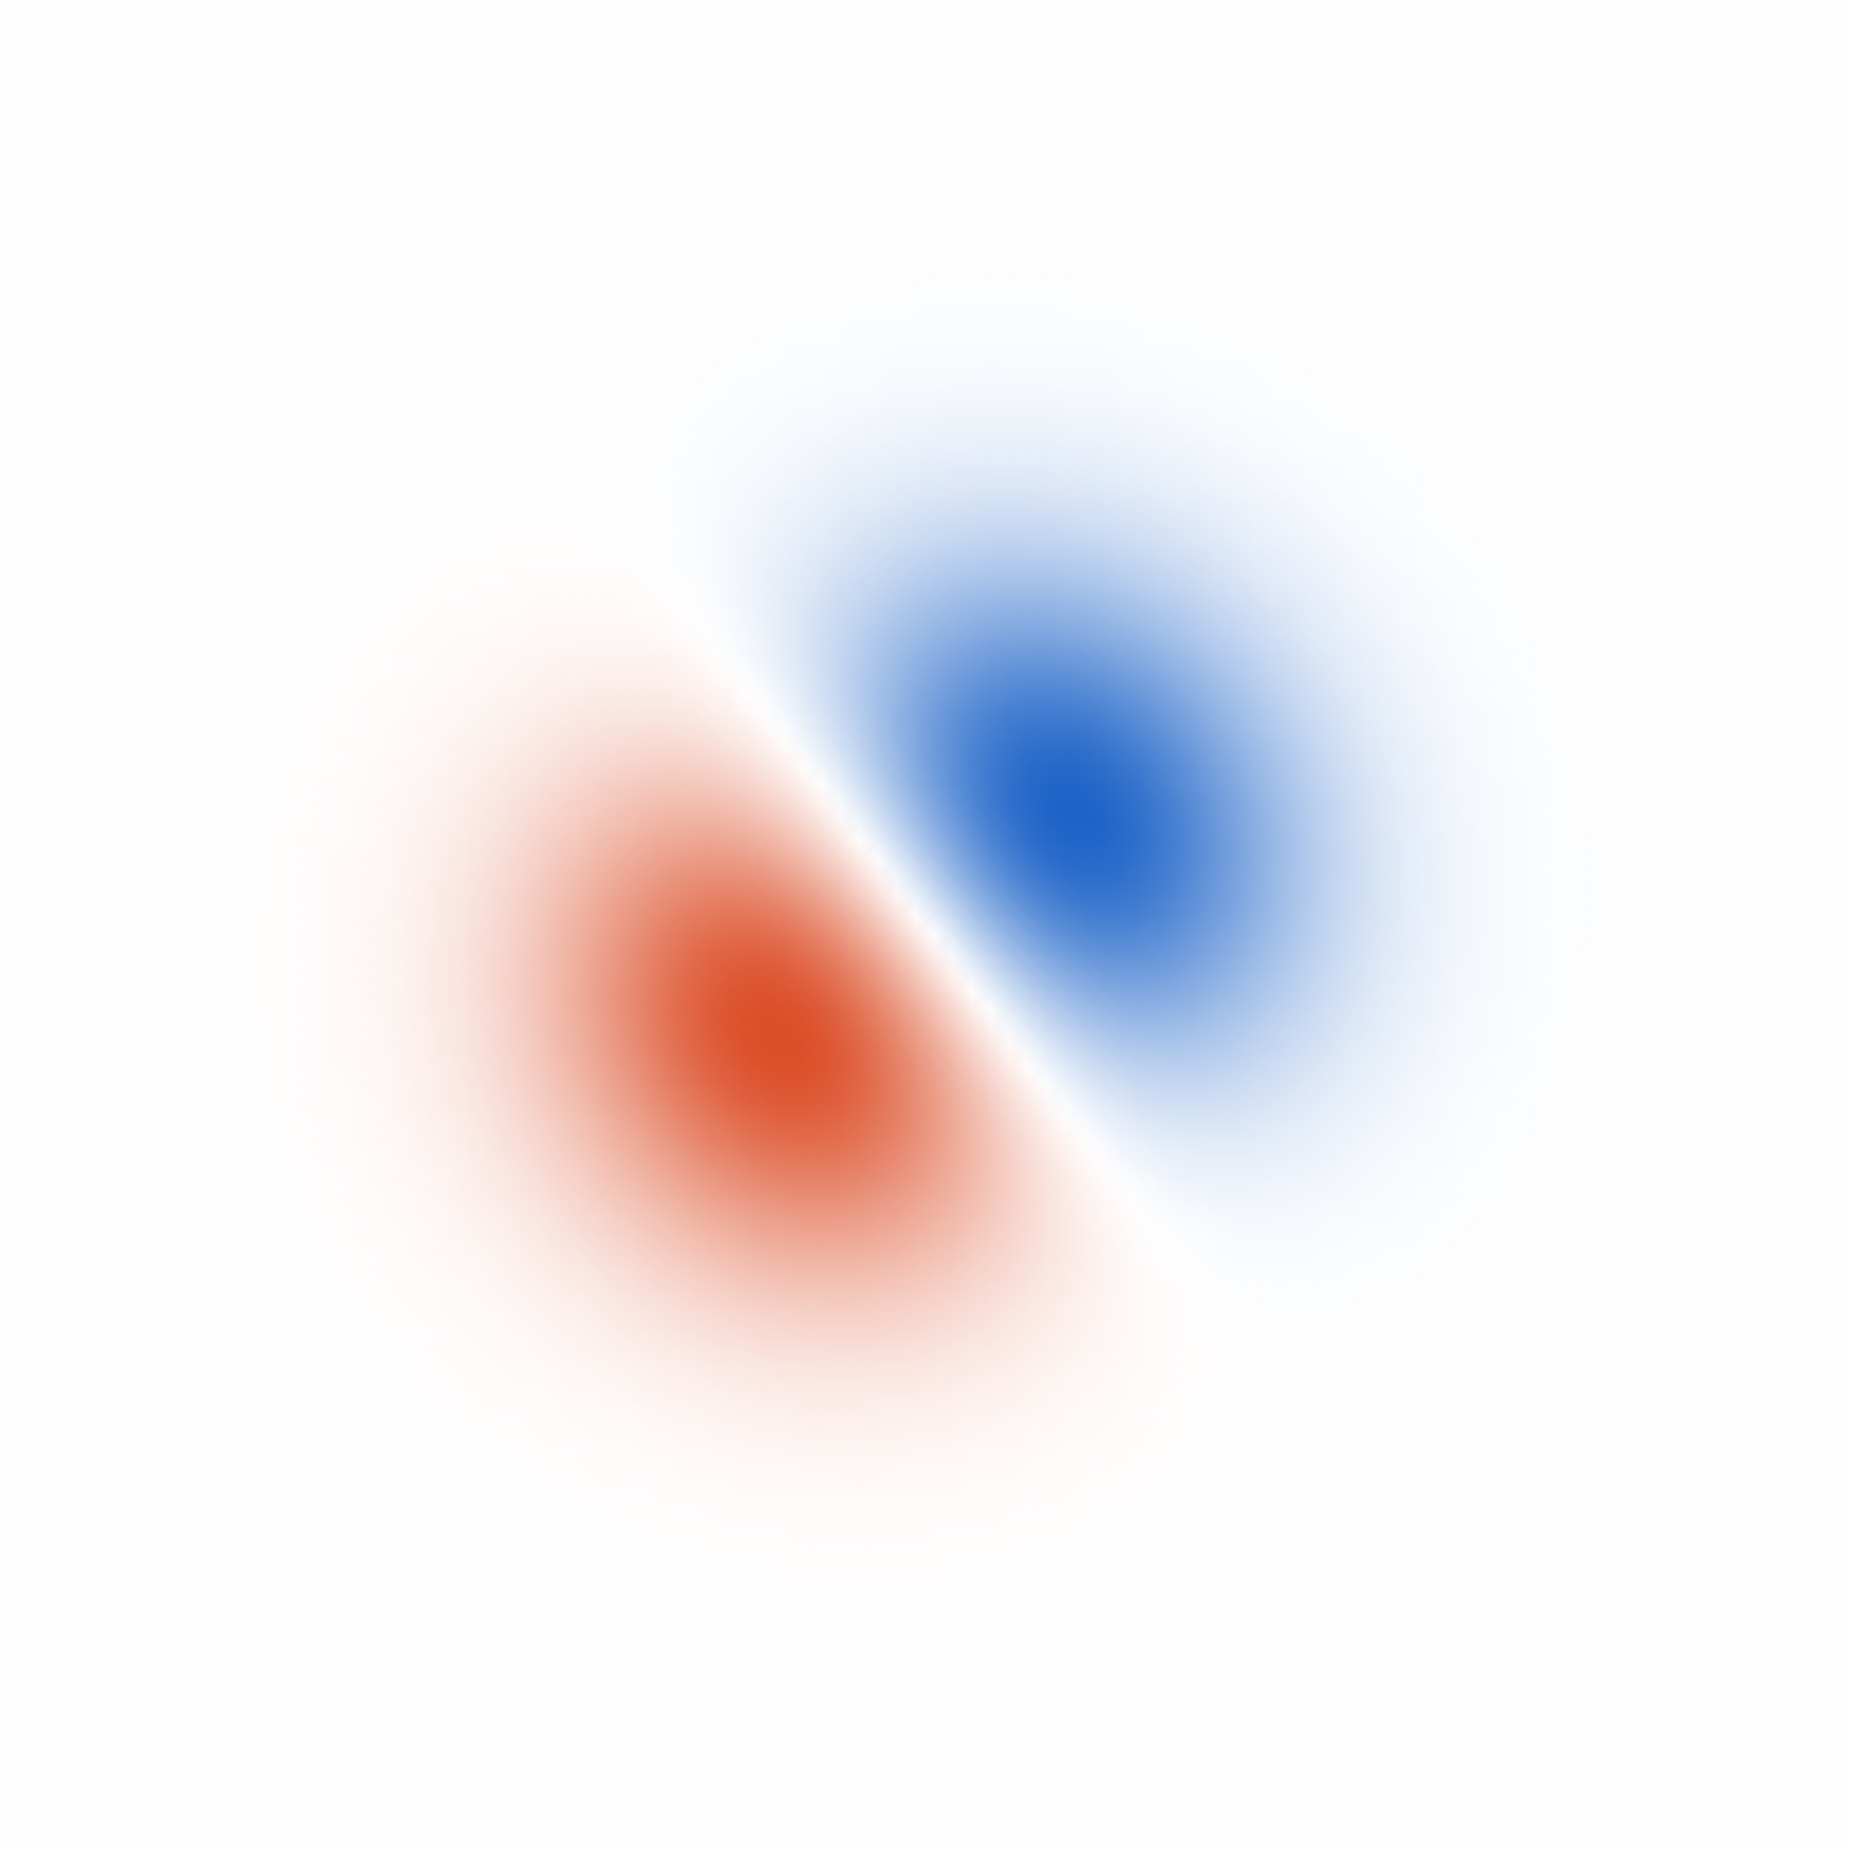
\includegraphics[width=\linewidth]{img/chapter3/counting/harmonic/4a.png}}} & $ \begin{matrix} \mathbf{u_{1,2}} \vspace{5pt}\\ \scalebox{1.5}{$\mathbf{2}$} \end{matrix} $ & \parbox[c]{\hoWidth}{\vspace{2pt}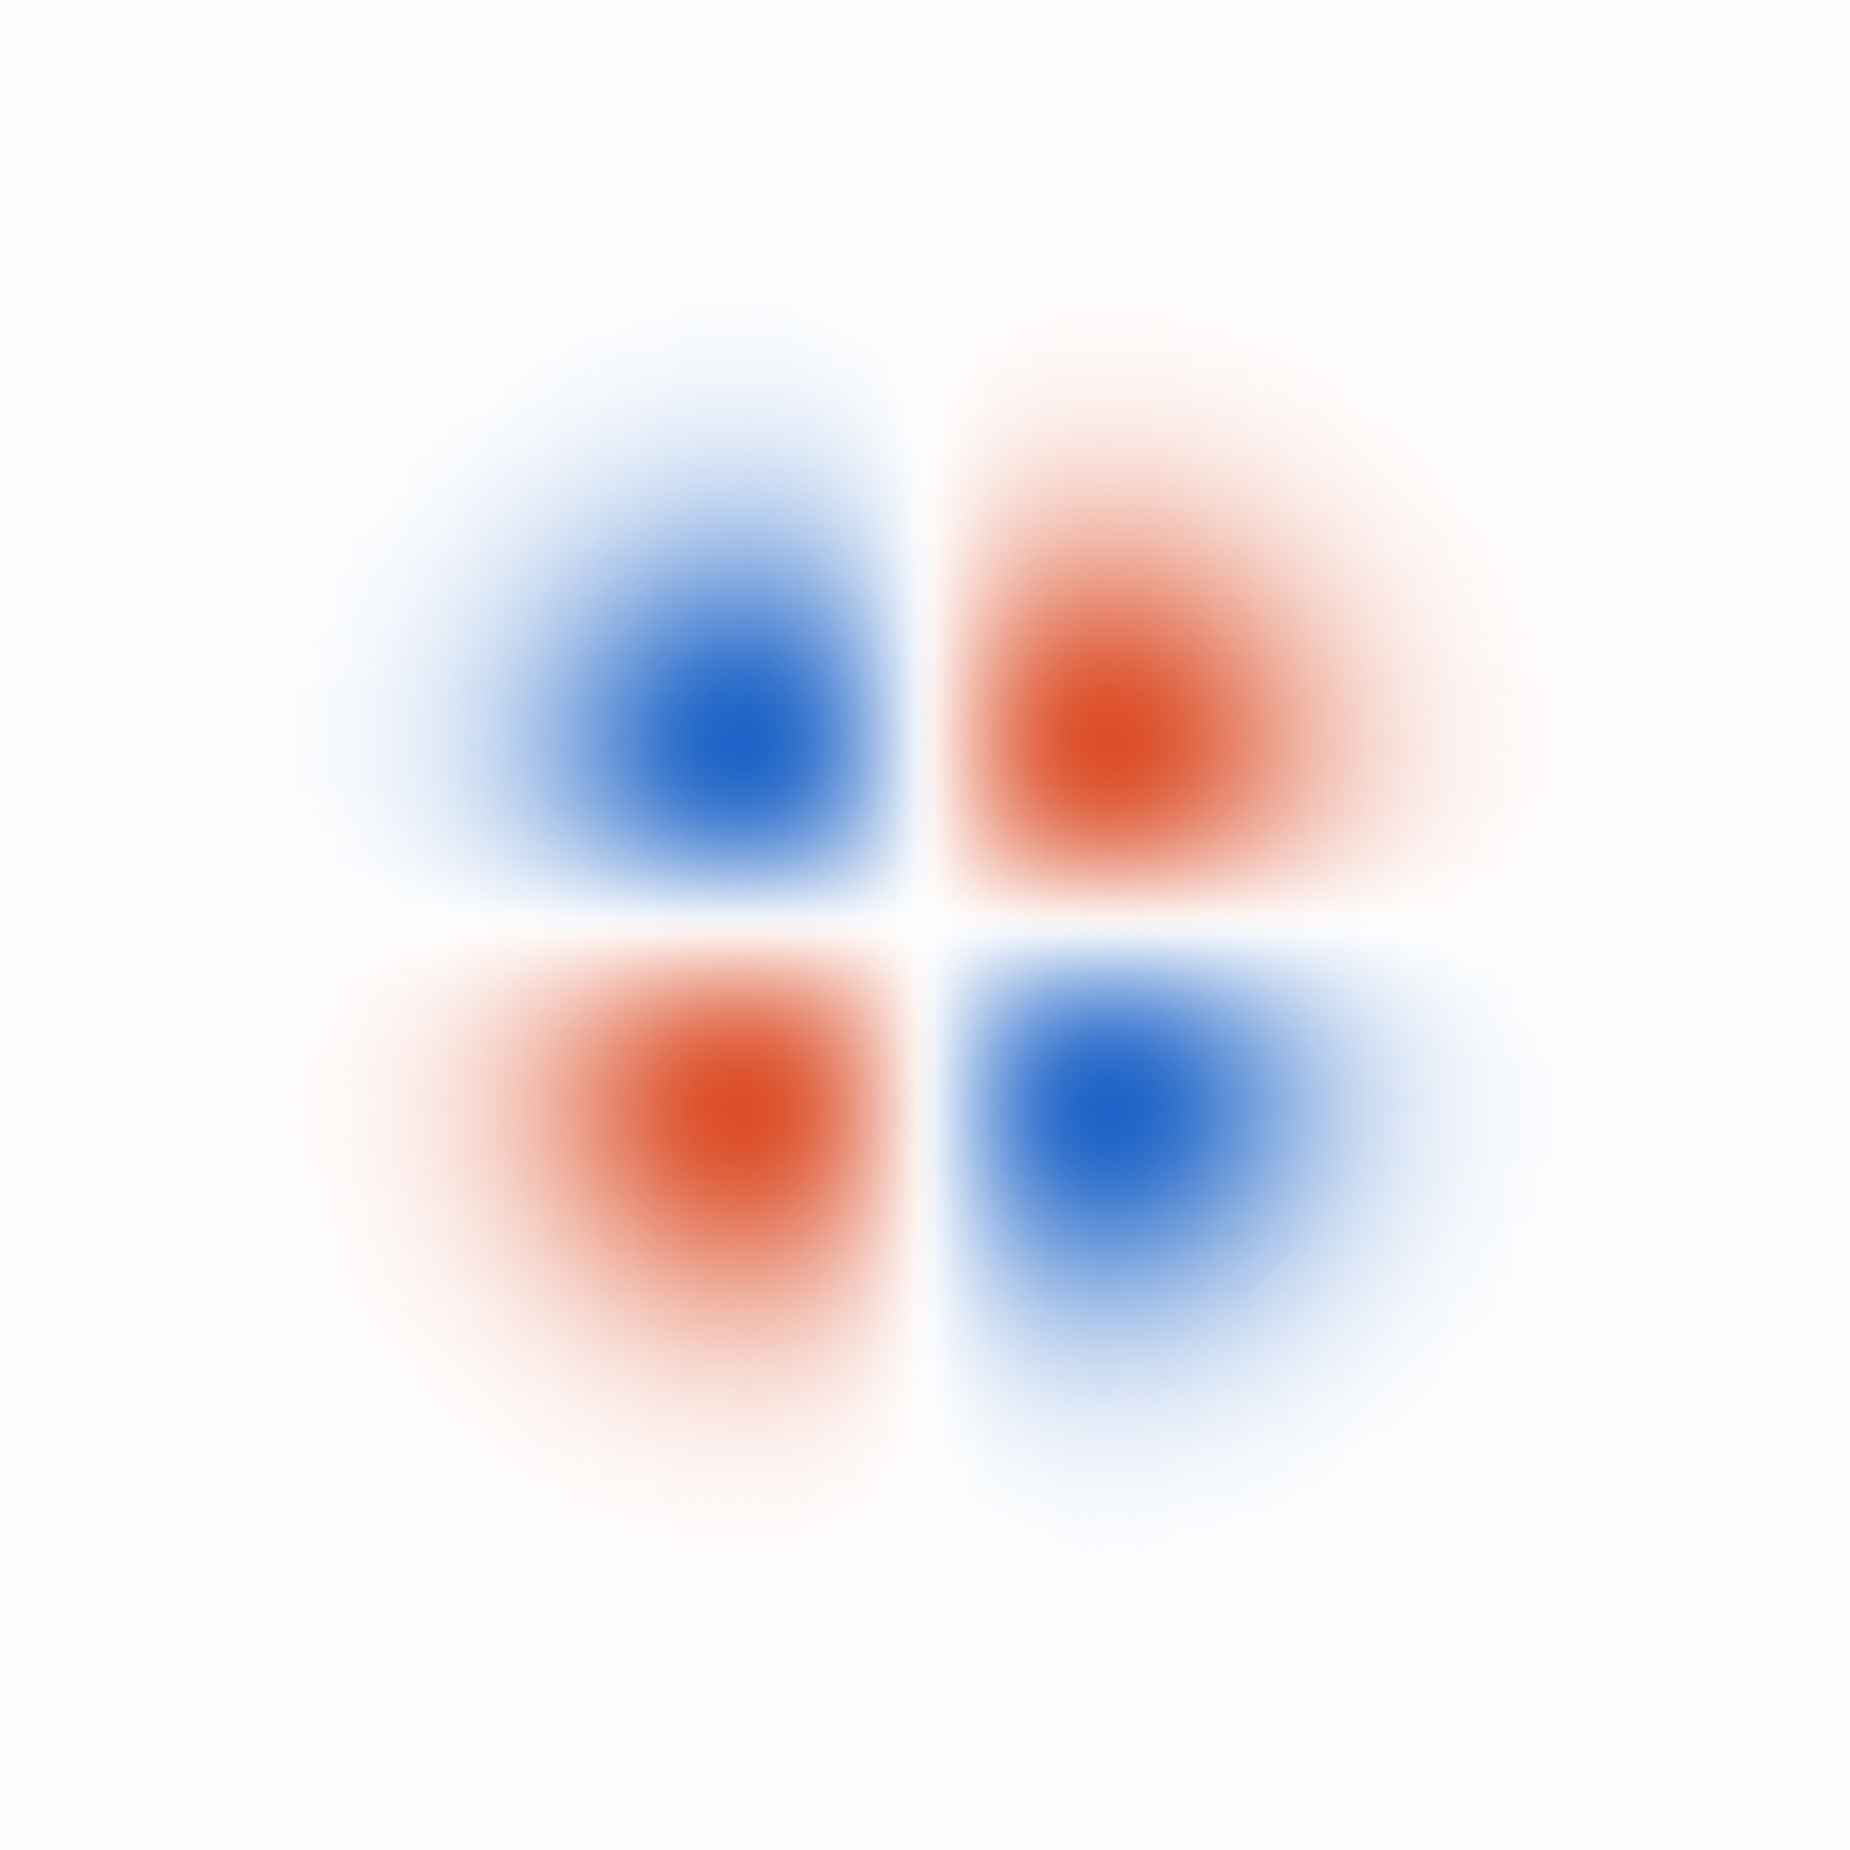
\includegraphics[width=\linewidth]{img/chapter3/counting/harmonic/6a.png}\vspace{2pt}} & $ \begin{matrix} \mathbf{u_{2,2}} \vspace{5pt}\\ \scalebox{1.5}{$\mathbf{4}$} \end{matrix} $  \\
      \cline{1-6}                                                                                                          &                                                      & \multicolumn{1}{|c}{\parbox[c]{\hoWidth}{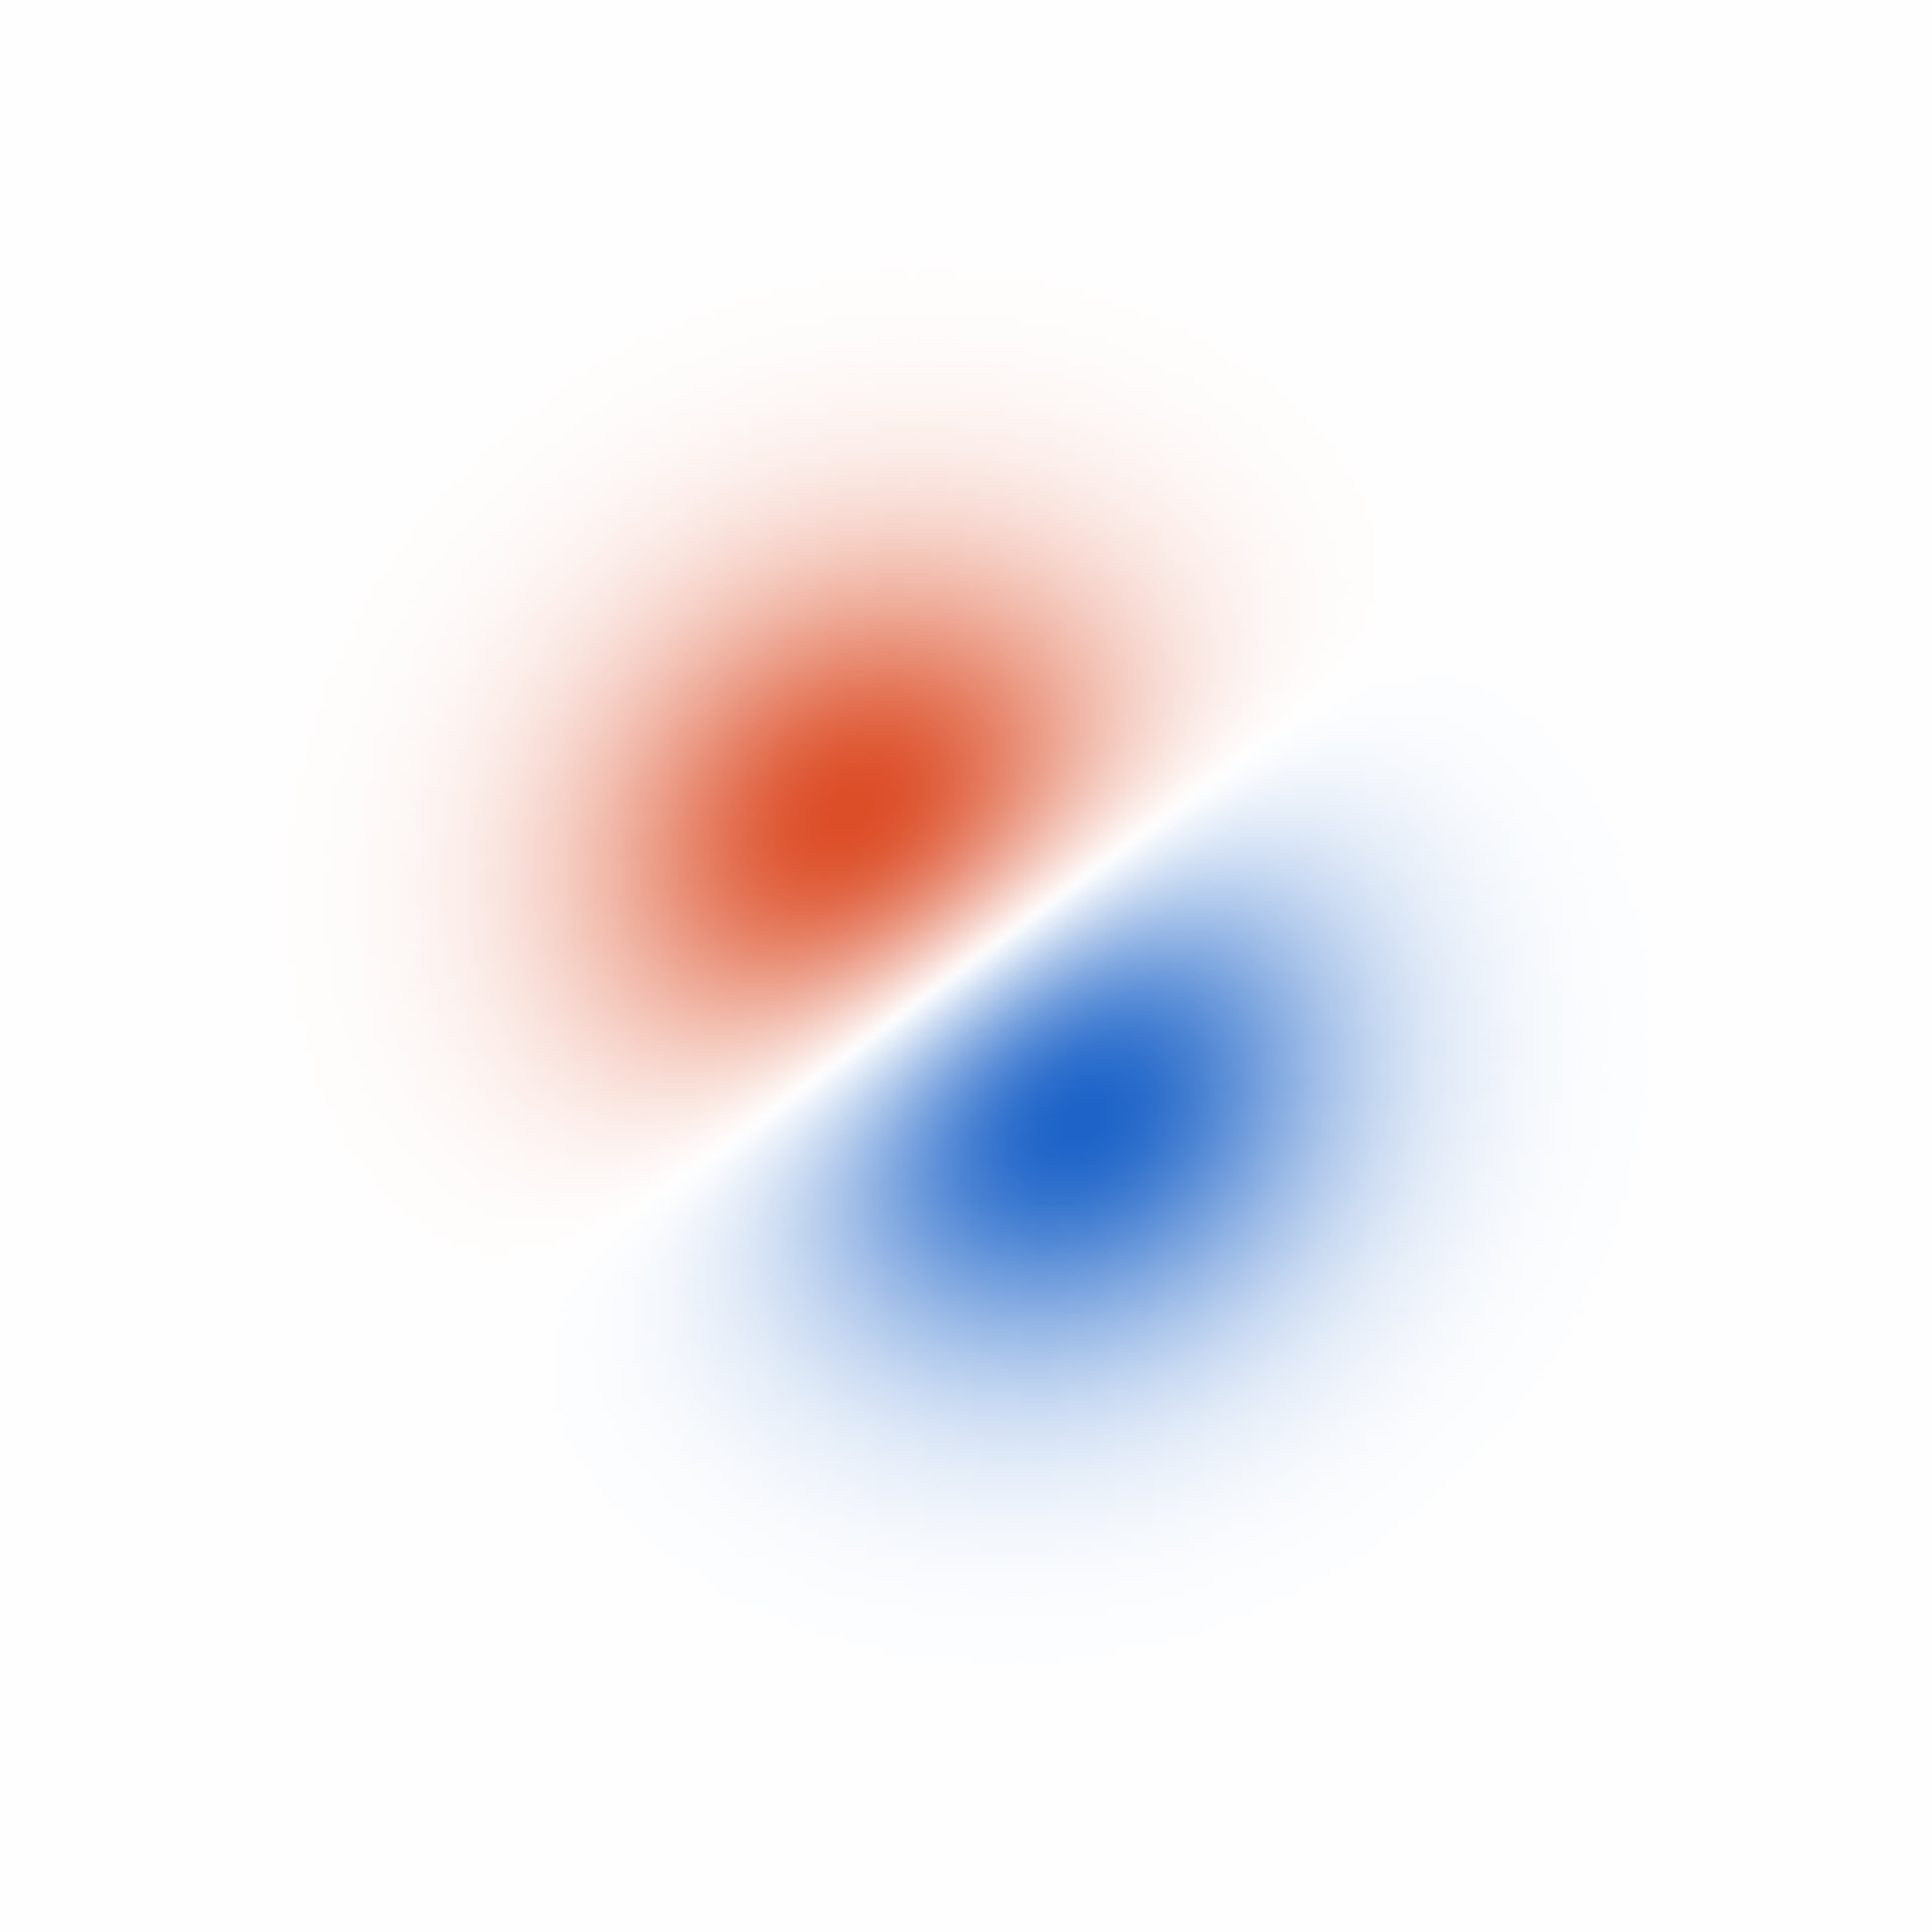
\includegraphics[width=\linewidth]{img/chapter3/counting/harmonic/4b.png}}} & $ \begin{matrix} \mathbf{u_{2,1}} \vspace{5pt}\\ \scalebox{1.5}{$\mathbf{2}$} \end{matrix} $ & \parbox[c]{\hoWidth}{\vspace{2pt}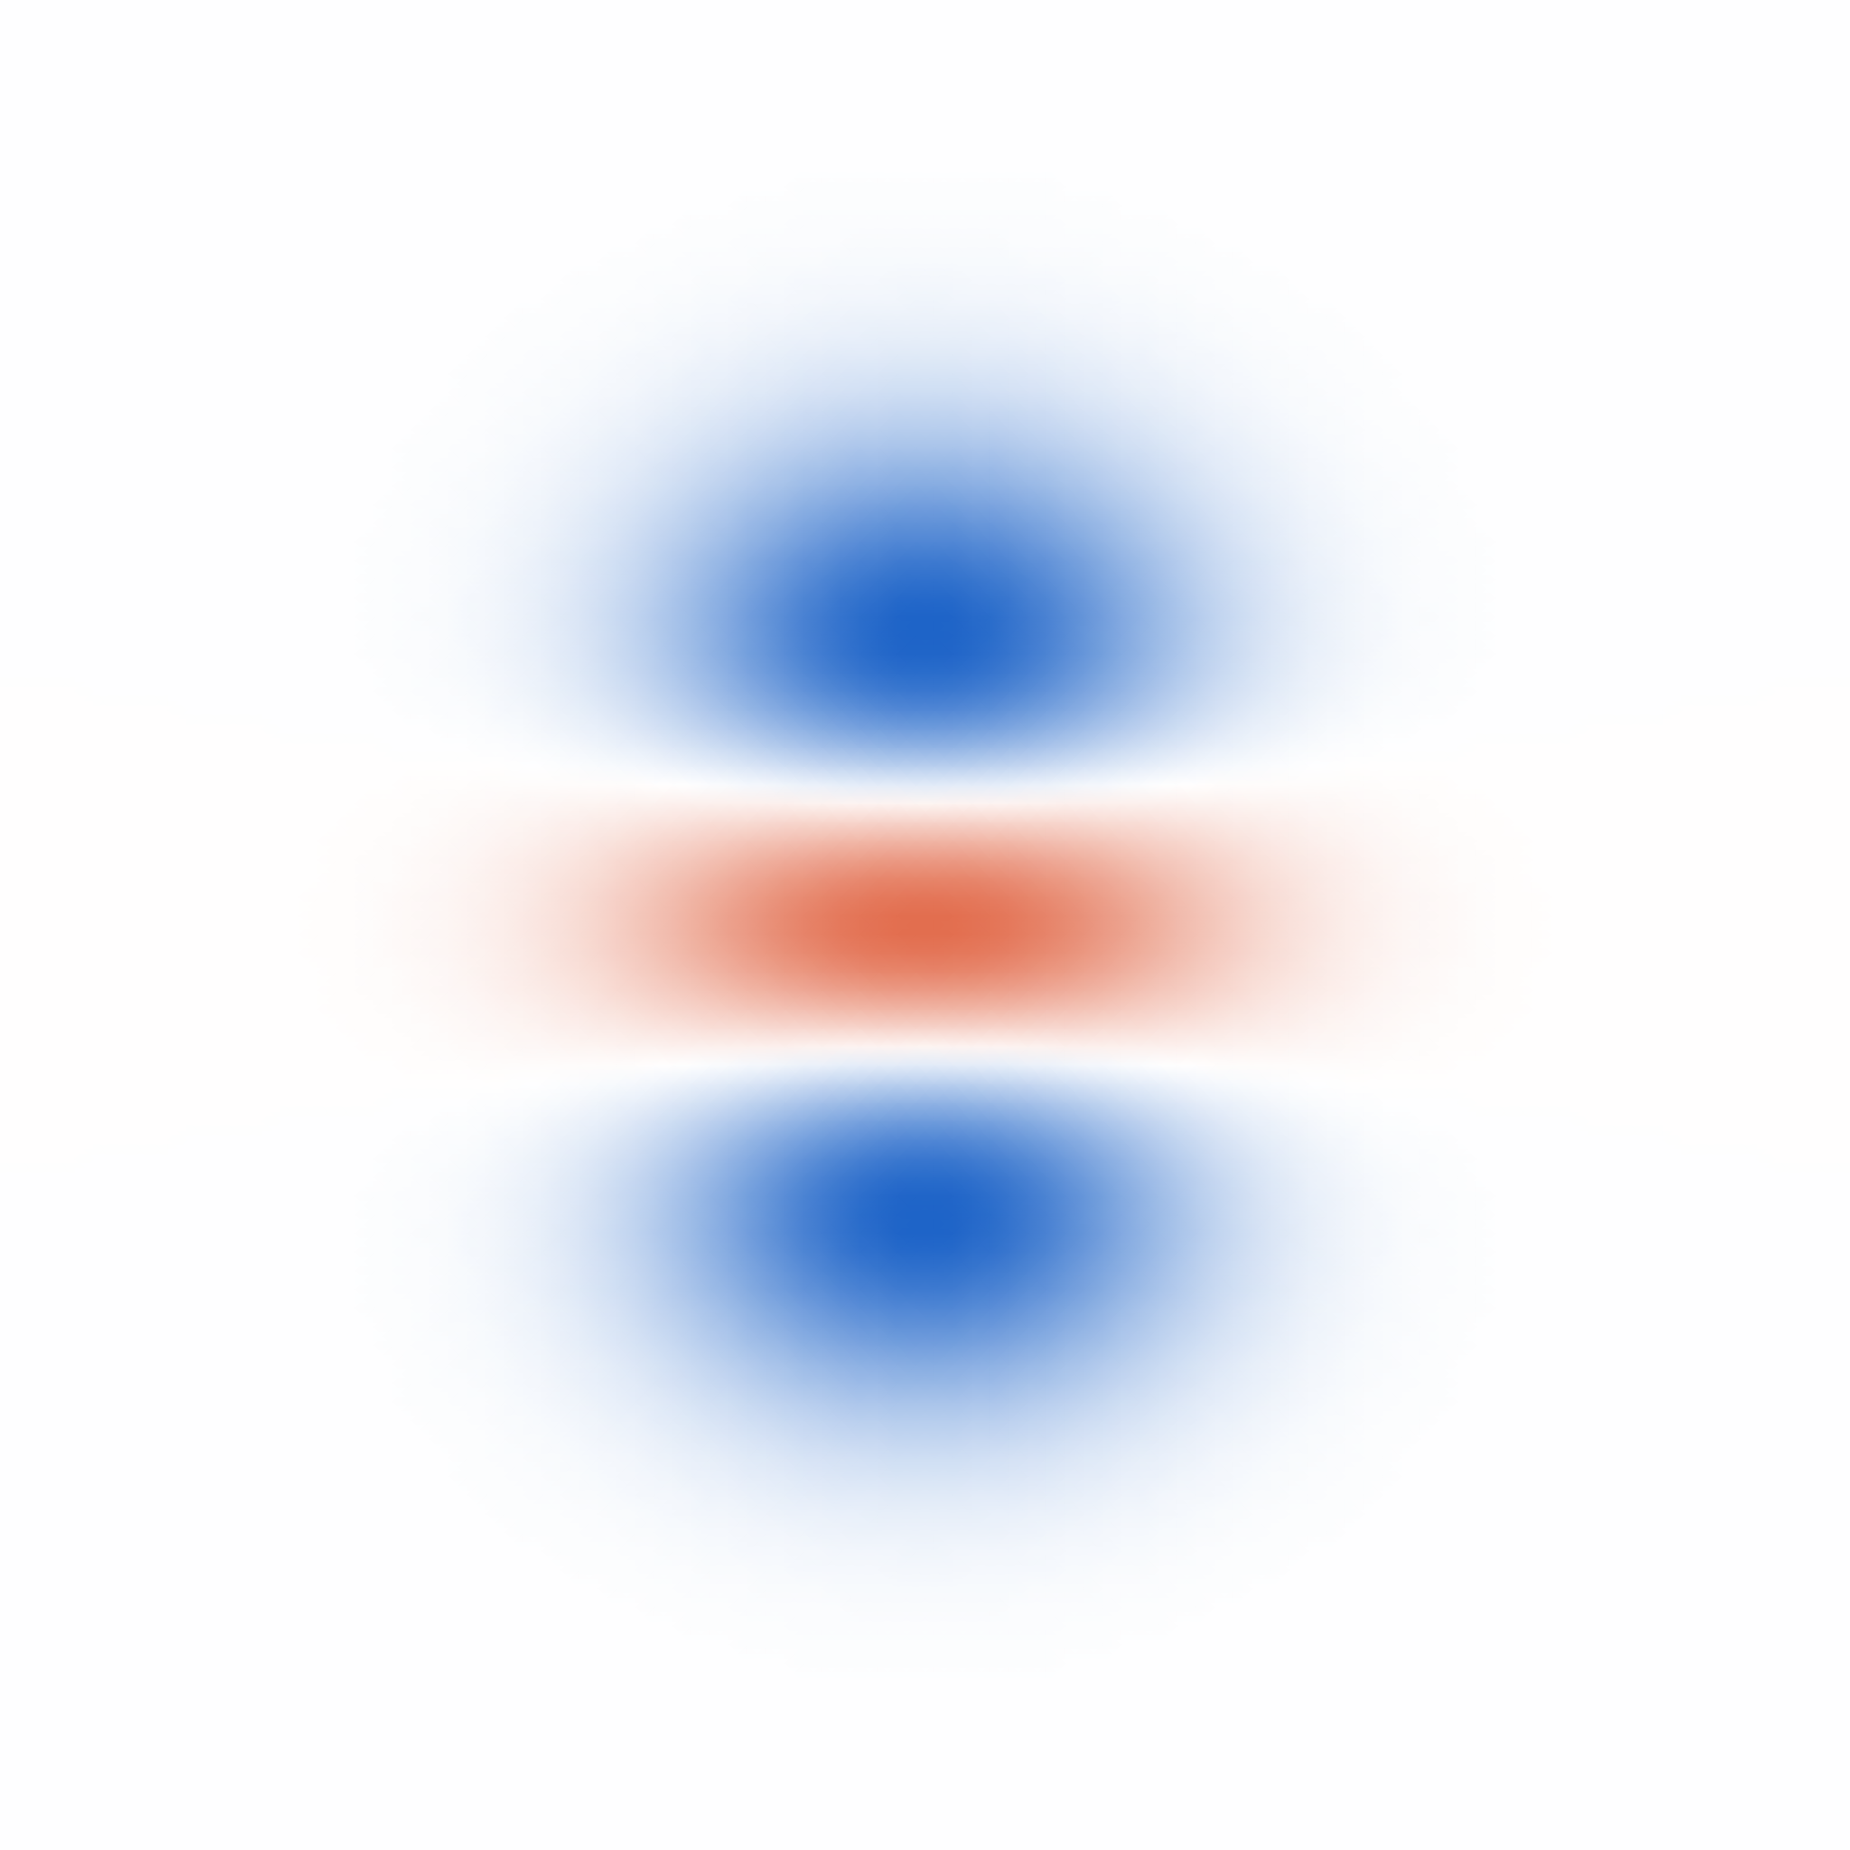
\includegraphics[width=\linewidth]{img/chapter3/counting/harmonic/6b.png}\vspace{2pt}} & $  \begin{matrix} u_{1,3} \vspace{5pt}\\ \scalebox{1.5}{$3$} \end{matrix} $ \\
      \cline{3-6}                                                                                                          &                                                      &                                                                                                                      &                                & \parbox[c]{\hoWidth}{\vspace{2pt}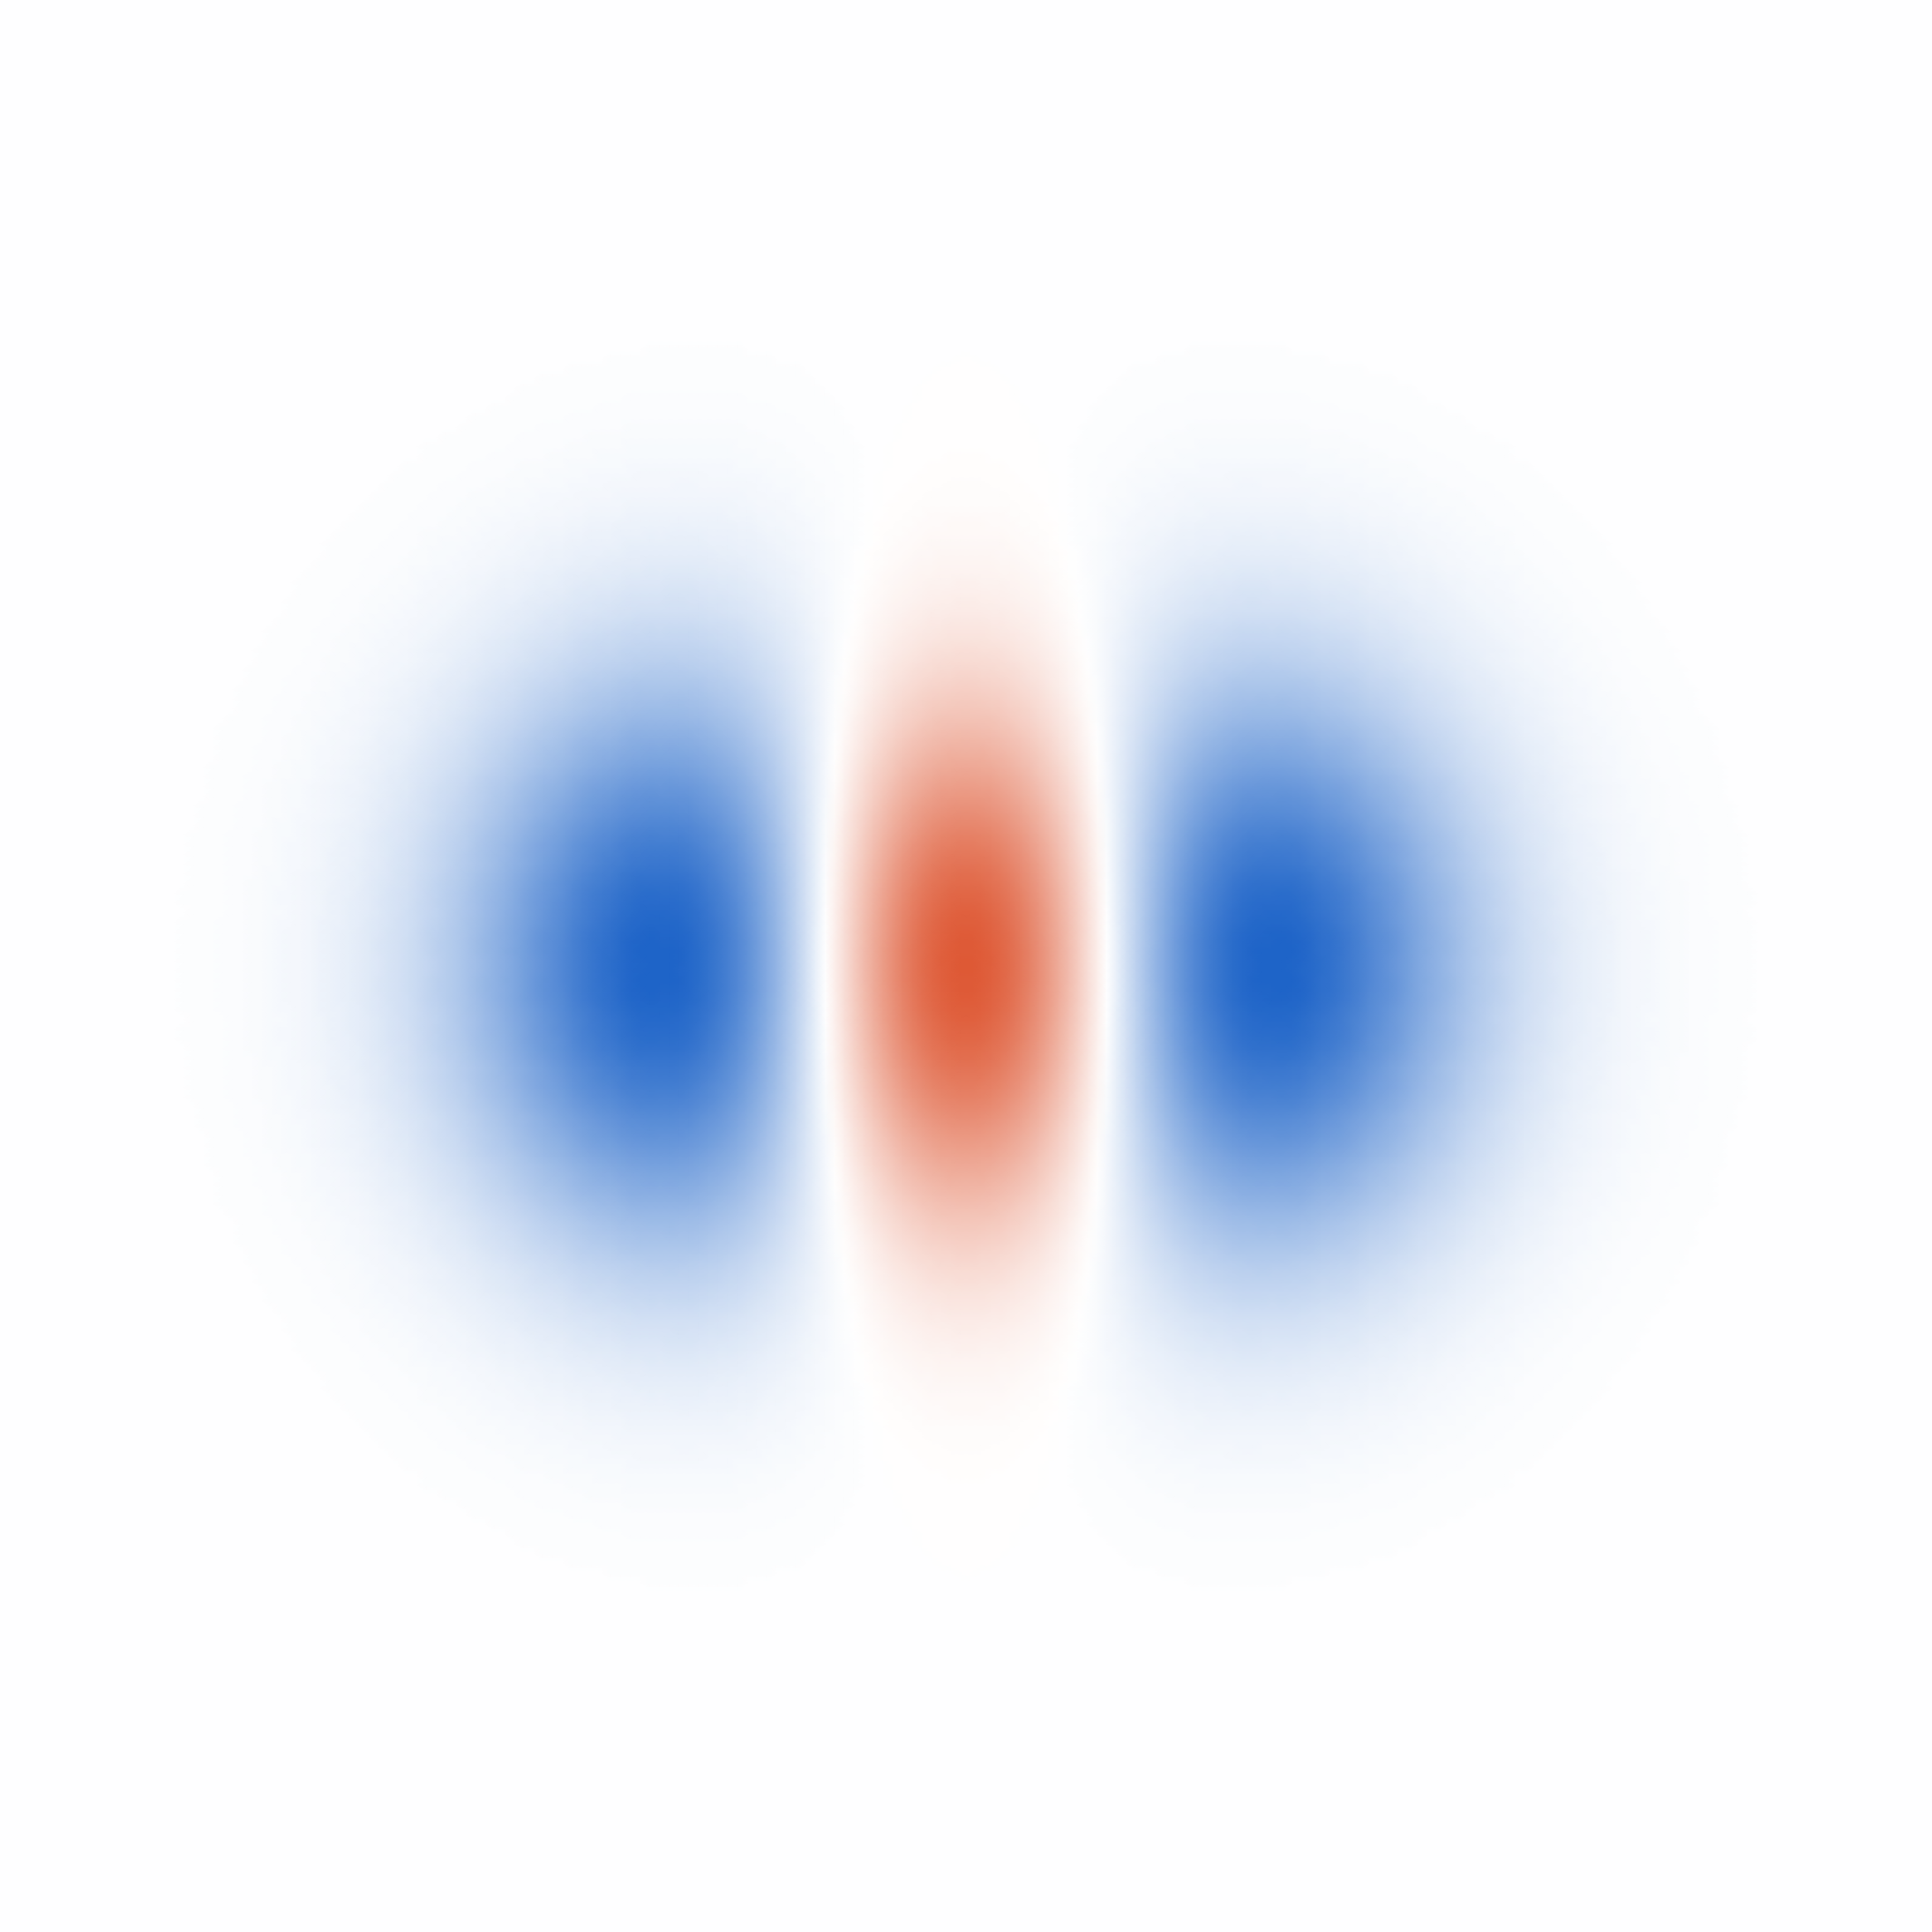
\includegraphics[width=\linewidth]{img/chapter3/counting/harmonic/6c.png}\vspace{2pt}} & $ \begin{matrix} u_{3,1} \vspace{5pt}\\ \scalebox{1.5}{$3$} \end{matrix} $  \\
      \cline{5-6}
    \end{tabular}
    \caption{\label{tab:courant_harmonic}Density plots (see also figure~\ref{fig:harmonic_3d}) of the first six eigenfunctions of the quantum harmonic oscillator, $-\nabla^2 u + (x^2+y^2) u = \lambda u$, on the square $[-5;5]\times [-5;5]$, with homogeneous Dirichlet boundary conditions. For each eigenfunction, the number of nodal domains is indicated. The eigenfunctions for which Courant's nodal domain theorem is strict, are highlighted in bold. These four eigenfunctions presented here are the only ones for which this strictness holds, for the harmonic oscillator. }
  \end{center}
\end{table}

Up until now, there was no method, that the authors know of, to reliably determine the exact number of eigenvalues lower than a given value $E$ for multidimensional problems. The best known result is already almost a century old: Courant's nodal domain theorem~\cite[vol I, chapter  VI, paragraph 2, theorem 2]{courant_methods_2008}\footnote{A more modern formulation of this theorem can be found in for example~\cite[theorem 1.1]{berard_nodal_2014}.}. This theorem states that, for an eigenfunction $u$ with corresponding eigenvalue $\lambda$, there are at least as many eigenvalues (counted with multiplicity) less than $\lambda$, as the number of nodal domains of $u$ minus one. A nodal domain is defined as a largest connected set of the domain on which the eigenfunction $u$ does not become zero. The nodal domain theorem gives, when an eigenvalue $\lambda$ with corresponding eigenfunction is known, a lower bound on the number of eigenvalues less than $\lambda$. However, only for restricted classes of one-dimensional problems, such as regular Sturm--Liouville problems with linear separated boundary conditions on bounded domains, this value is exact. In table~\ref{tab:courant_harmonic}, this fact is demonstrated by showing that the number of nodal domains of an eigenfunction does not lead to an exact estimate for the index of the corresponding eigenvalue.
% Fun fact: Richard Courant maried the daughter of Carl Runge

\begin{figure}
  \begin{center}
    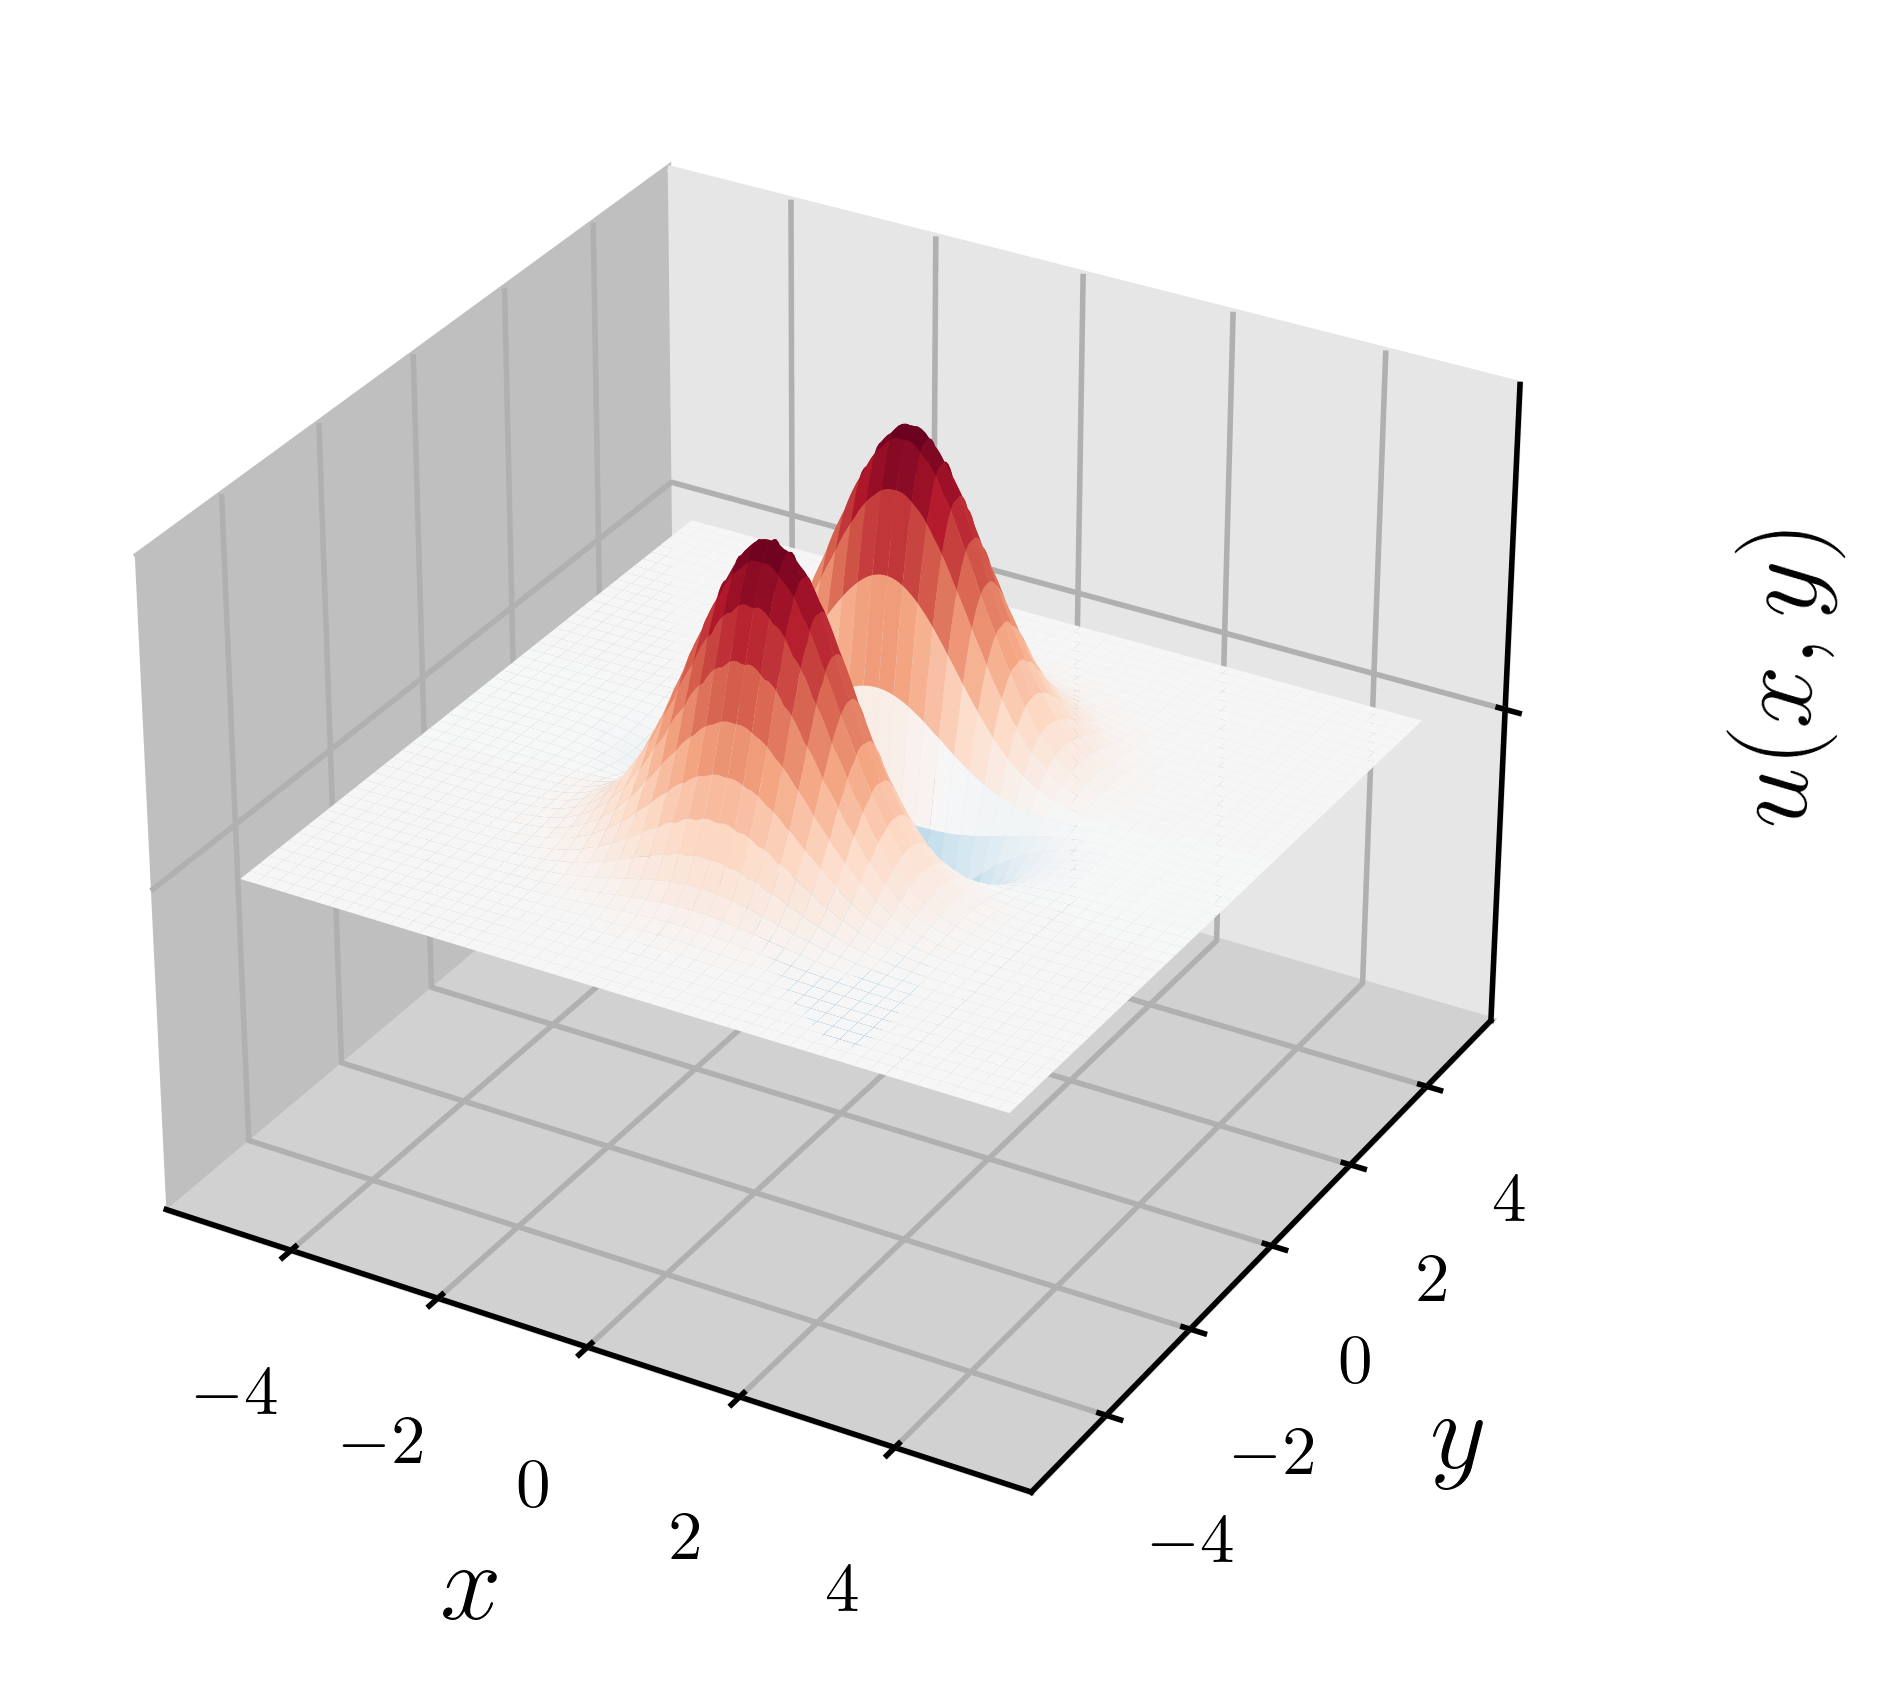
\includegraphics[width=\linewidth]{img/chapter3/counting/harmonic_3d.png}
    \caption{\label{fig:harmonic_3d} A three-dimensional graph of the eigenfunction $u_{3,1}$ of the quantum harmonic oscillator $-\nabla^2 u + (x^2+y^2) u = \lambda u$, on the square $[-5; 5] \times [-5; 5]$, with homogeneous Dirichlet boundary conditions. This graph illustrates how the density plots from table~\ref{tab:courant_harmonic} and figure~\ref{fig:c3_disc_solutions} should be interpreted.}
  \end{center}
\end{figure}

A practical problem in applying Courant's nodal domain theorem is that numerically, it is quite difficult to reliably determine the number of nodal domains of a function. This motivated us to formulate theorem~\ref{lem:c3_eigenvalues_curves}.

To develop the theoretical framework for this theorem, some definitions are needed. These will simplify the notation and proof of our results.
\begin{definition}
  The one-dimensional cross-section $l_{\Omega,i}(\vb{x})$ of a Lipschitz domain $\Omega$ along the $i^\text{th}$ dimension through $\vb{x}$ is defined as:
  $$
    l_{\Omega,i}(\vb{x}) := \left\{\vb{y} \in \Omega \ |\  \forall j \in \{1, \dots, n\} \setminus \{i\} : \vb{x}_j = \vb{y}_j   \right\}\text{.}
  $$
\end{definition}

Note that, when $\Omega$ is bounded, $l_{\Omega,i}(\vb{x})$ is the union of collinear line segments. As such, the following definition represents the maximal sum of the lengths of each of these segments.

\begin{definition}
  The \emph{directional diameter}, $\dirdiam_i(\Omega)$, of a bounded Lipschitz domain $\Omega \subseteq \RR^n$ is defined as:
  $$
    \dirdiam_i(\Omega) := \sup_{\vb{x}\in\Omega} \int_{-\infty}^{\infty} I_\Omega(\vb{x}_1, \dots, \vb{x}_{i-1}, t, \vb{x}_{i+1}, \dots, \vb{x}_n) \, \dd t \text{.}
  $$
  Here $I_\Omega(\vb{x})$ is defined as $1$ if $\vb{x} \in \Omega$ and zero otherwise.
\end{definition}

In theorem~\ref{the:c3_counting_eigenvalues}, we will be able to identify each eigenvalue by using a continuous sequence of domains $\Omega_\epsilon$. For this sequence of domains, it should hold that if $\epsilon \to 0$, the domains should become unboundedly small. The notion of the \emph{directional diameter} allows us to quantify this.

\begin{figure}[t]
  \begin{center}
    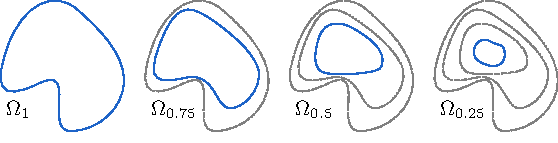
\includegraphics[width=\linewidth]{img/chapter3/counting/main-theorem-omega.pdf}
    \caption{\label{fig:intuitive_example_omega} An example of a sequence of domains $\Omega_\epsilon$ that satisfy the necessary conditions for theorem~\ref{the:c3_counting_eigenvalues}: the domains are nested, all domains are Lipschitz, and the horizontal as well as the vertical directional diameter converge to zero for $\epsilon \to 0^{+}$.}
  \end{center}

  \begin{center}
    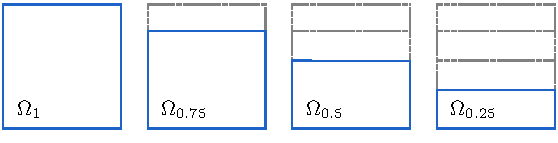
\includegraphics[width=\linewidth]{img/chapter3/counting/main-theorem-rho.pdf}
    \caption{\label{fig:intuitive_example_rho} Another example of a sequence of domains $\Omega_\epsilon$ that also satisfy the necessary conditions for theorem~\ref{the:c3_counting_eigenvalues}. Note that these conditions only require that any directional diameter converges to zero. In this example, the horizontal directional diameter does not converge to zero: $\lim_{\epsilon \to 0^+}\dirdiam_1(\Omega_\epsilon) \neq 0$. The vertical directional diameter does vanish: $\lim_{\epsilon \to 0^+}\dirdiam_2(\Omega_\epsilon) = 0$.}
  \end{center}
\end{figure}

In figures~\ref{fig:intuitive_example_omega} and~\ref{fig:intuitive_example_rho}, two examples of series of domains are given. Both of these sets of domains are applicable for theorem~\ref{the:c3_counting_eigenvalues}. We would like to note that the domain from figure~\ref{fig:intuitive_example_rho} is particularly valuable for~\cite{ixaru_new_2010,baeyens_improvements_2022}.

The next section will be dedicated to proving this theorem. In the last section, we will provide some examples of and motivation for our work.


\subsection{The main theorem} \label{sec:main_theorem}

Throughout this section, the $L^2$-norm $\|\cdot\|_{L^2(\Omega)}$ and Sobolev norm $\|\cdot\|_{H^k(\Omega)}$ are being used. For clarity, we will provide the necessary definitions. For a more thorough discussion of these norms and their properties, many texts are available, for example~\cite{adams_sobolev_2003}.

Let $L^2(\Omega)$ be the space of functions $u : \Omega \to \RR$ such that the norm
$$
  \|u\|_{L^2(\Omega)} := \left(\int_\Omega \left| u \right|^2 \right)^{\frac{1}{2}}
$$
exists and is finite.

The Sobolev space $ H^k(\Omega) = W^{k, 2}(\Omega) $ is the space of all functions $u \in L^2(\Omega)$ such that, for the multi-index $\alpha$ with order $|\alpha|$ at most $k$, each weak partial derivative $D^\alpha u$ of $u$ is a function in $L^2(\Omega)$. The Sobolev norm of $u$ is defined as:
$$
  \|u\|_{H^k(\Omega)} := \left(\sum_{|\alpha| \leq k} \int_\Omega \left| D^\alpha u \right|^2\right)^{\frac{1}{2}}\text{.}
$$

The function space $C^\infty(\Omega)$ consists of all infinitely differentiable functions defined on $\Omega$, and $C_0^\infty(\Omega)$ consists of all infinitely differentiable functions $f$ defined on $\Omega$ such that $f(\vb{x}) = 0$ for all $\vb{x} \in \dOmega$.

The subspace $ H^k_0(\Omega)$ of $H^k(\Omega)$ is the closure of $C_0^\infty(\Omega)$ in $H^k(\Omega)$.

Before proving the main theorem of this section, we provide a kind of Fried\-richs's inequality to estimate a lower bound for $\| u \|_{H^k(\Omega)}$ in terms of $\| u \|_{L^2(\Omega)}$, and the diameter\footnote{The diameter of a domain $\Omega$ is defined as $\diam\Omega := \sup_{\vb{x},\vb{y}\in \Omega} \|\vb{x} - \vb{y}\|_2$.} and any directional diameter of $\Omega$.

\begin{lemma}
  \label{lem:friederichs_like}
  Let $\Omega \subset \RR^n$ be a bounded domain with Lipschitz boundary, and $k \in \mathbb{N}^{+}$. For each $u \in H_0^k(\Omega)$, and any $j \leq n$
  \begin{equation}
    \label{equ:friederichs_like}
    \| u \|_{L^2(\Omega)} \leq \sqrt{\diam(\Omega) \dirdiam_j(\Omega)} \| u \|_{H^k(\Omega)} \text{.}
  \end{equation}
\end{lemma}
\begin{proof}
  For ease of notation, we will assume $j = 1$. Note that this proof is equally valid for any other $j$. Assume also $u \in C^\infty_0(\Omega) \cap H_0^k(\Omega)$. Because of the homogeneous Dirichlet boundary conditions,
  the fundamental theorem of calculus\footnote{The fundamental theorem of calculus states that if $f : \RR \to \RR$ is a continuous and differentiable function with $f'(x)$ integrable then
    $$
      \int_a^b f'(x) \, \dd x = f(b) - f(a)\text{.}
    $$} can be used to estimate $|u(\vb{x})|^2$ for each $\vb{x} = (x_1, \dots, x_n) \in \Omega$
  $$
    \left|u(\vb{x})\right|^2 = \left|\int_{-\infty}^{x_1} \pdv[]{u}{x_1}\left(t, x_2, \dots, x_{n}\right)I_\Omega(t,x_2, \dots, x_n)\dd t\right|^2 \text{.}
  $$
  In this formula, and throughout the proof, we formally pose that $u(\vb{x}) \equiv 0$ for $\vb{x} \notin \Omega$. Note that the fundamental theorem of calculus is applicable because $u$ is compactly supported and in $C^1(\Omega)$.

  Applying the Cauchy--Schwarz inequality provides some simplifications. Extending the integration domain removes the dependency on $x_1$.
  \begin{align*}
    \left|u(\vb{x})\right|^2 & \leq \int_{-\infty}^{x_1} I_\Omega(t,x_2, \dots, x_n) \dd t \int_{-\infty}^{x_1} \left|\pdv[]{u}{x_1}\left(t,x_2, \dots, x_n\right)\right|^2\dd t \\
                             & \leq \dirdiam_1(\Omega) \int_{a}^{b} \left|\pdv[]{u}{x_1}\left(t, x_2, \dots, x_n\right)\right|^2\dd t
  \end{align*}
  with $a = \inf_{\vb{x} \in \Omega}\{\vb{u}_1 \,|\, \vb{u} \in l_{\Omega, 1}(\vb{x})\}$ and $b = \sup_{\vb{x} \in \Omega}\{\vb{u}_1 \,|\, \vb{u} \in l_{\Omega, 1}(\vb{x})\}$. Integrating both sides over $\Omega$, applying Fubini's theorem\footnote{Fubini's theorem allows (under some easily checked conditions) to reorder the integration order in multidimensional integrals.}, and noting that $b - a \leq \diam(\Omega)$, yields the required expression for $u \in C^\infty_0(\Omega)$.
  \begin{align*}
    \|u\|_{L^2(\Omega)}^2 & \leq \dirdiam_1(\Omega) \int_\Omega \int_{a}^{b} \left|\pdv[]{u}{x_1}\left(t, x_2, \dots, x_{n}\right)\right|^2\dd t \, \dd \vb{x} \\
                          & = \dirdiam_1(\Omega) \, (b - a) \, \int_{\Omega} \left|\pdv[]{u}{x_1}\left(\vb{x}\right)\right|^2 \dd \vb{x}                       \\
                          & \leq \dirdiam_1(\Omega) \, \diam(\Omega) \, \| u \|^2_{H^k(\Omega)}\text{.}
  \end{align*}

  To prove this for each $u \in H_0^k(\Omega)$, we only have to note that
  $C^\infty_0(\Omega)$ is $H^k(\Omega)$-dense in $H^k_0(\Omega)$. Now $u \in H_0^k(\Omega)$ can be written as $u = \lim_{i \to +\infty} u_i$ with $u_i \in C^\infty_0(\Omega)$. This implies that
  $$\|u\|_{L^2(\Omega)}^2 \leq \dirdiam_1(\Omega) \, \diam(\Omega) \, \| u \|^2_{H^k(\Omega)}\text{,}$$
  for each $u \in H_0^k(\Omega)$.
\end{proof}

Now we are able to prove lemma~\ref{lem:c3_eigenvalues_curves}. This prepares the main result of this section: theorem~\ref{the:c3_counting_eigenvalues}.

\begin{lemma}\label{lem:c3_eigenvalues_curves}
  Let $\left\{\Omega_\epsilon \subseteq \RR^n \ | \ \forall \epsilon \in \left]0, 1\right]\right\}$ be a continuous family of diffeomorphic bounded Lipschitz domains, such that $ a < b \implies \Omega_a \subsetneq \Omega_b $, and
  $$
    \exists j\in\{1,\dots, n\} : \lim_{\epsilon \to 0^{+}} \dirdiam_j(\Omega_\epsilon) = 0\text{.}
  $$

  Let $\mathcal{L}$ be a linear self-adjoint uniformly elliptic operator, defined on $\Omega_1$. Define $\lambda_{\epsilon,i}$ as the $i^\text{th}$ eigenvalue of $\mathcal{L}$ limited to $\Omega_\epsilon$ with homogeneous Dirichlet boundary conditions. Then for each $i \in \mathbb{N}$, the values $\lambda_{\epsilon,i}$ as functions of $\epsilon$
  \begin{itemize}
    \item are continuous,
    \item are strictly decreasing,
    \item and are unbounded for $\epsilon \to 0^{+}$.
  \end{itemize}
\end{lemma}
\begin{proof}
  Already in 1924, Courant and Hilbert~\cite[vol I. chapter V. paragraph 13]{courant_methods_2008} noted the continuity of the spectrum under perturbations of the elliptic operator. Hale described (e.g.~\cite{hale_eigenvalues_2005}) how to translate regular perturbations in the domain to perturbations in the operator. Our set of diffeomorphic domains satisfies the necessary assumptions formulated by Hale, so continuity is guaranteed.

  That $\lambda_{\epsilon, i}$ is a decreasing function of $\epsilon$ can be shown by application of~\cite[vol I, chapter  VI, paragraph 2, theorem 3]{courant_methods_2008} \emph{``Under the boundary condition $u = 0$ the $n^\text{th}$ eigenvalue for a domain $G$ never exceeds the $n^\text{th}$ eigenvalue for a subdomain of $G$".} The strictness is addressed in a footnote by this theorem: \emph{"In fact, it is always smaller when we are dealing with a proper subdomain."}.

  To prove that $\lambda_{\epsilon, i}$ grows unboundedly, we start with Gårding's inequality~\cite[section 9.2.3]{renardy_introduction_2004}. It says that there exist $C_1$ and $C_2$ such that for all $u \in H^k_0(\Omega_\epsilon)$:
  \begin{equation}\label{equ:garding}
    \frac{\bra{\mathcal{L}u}\ket{u}_{L^2(\Omega_\epsilon)}}{\|u\|_{L^2(\Omega_\epsilon)}^2} + C_1 \geq C_2 \frac{\|u\|_{H^k(\Omega_\epsilon)}^2}{\|u\|_{L^2(\Omega_\epsilon)}^2}\text{.}
  \end{equation}
  Note that the same $C_1$ and $C_2$ as for $\Omega_1$ will also work for $\Omega_\epsilon$. Lemma~\ref{lem:friederichs_like} provides an estimate for the right-hand side of~\eqref{equ:garding}, which, in turn, provides an estimate for the operator $\mathcal{L}$:
  $$
    \frac{\bra{\mathcal{L}u}\ket{u}_{L^2(\Omega_\epsilon)}}{\|u\|_{L^2(\Omega_\epsilon)}^2} \geq \frac{C_3}{\sqrt{\dirdiam_j(\Omega_\epsilon)}} - C_1\text{,}
  $$
  for a constant $C_3$. By assumption the right-hand side is unbounded for $\epsilon \to 0$. Substituting the eigenfunction $u_{\epsilon, i}$, corresponding to the eigenvalue $\lambda_{\epsilon, i}$, into the left-hand side yields that $\lambda_{\epsilon, i}$ has to be unbounded as well.
\end{proof}

\begin{figure}
  \begin{center}
    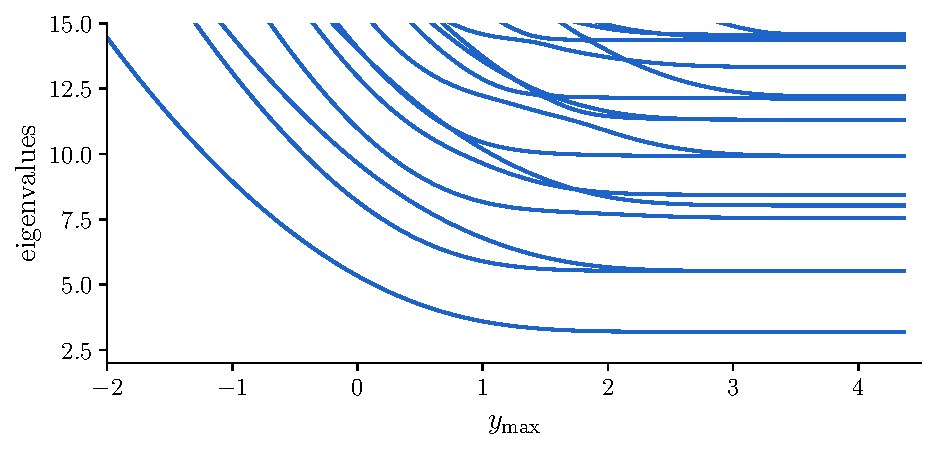
\includegraphics[width=\textwidth]{img/chapter3/counting/counting_eigenvalues.pdf}
    \caption{This graph displays all eigenvalues less than $15$ for the two-dimensional Schrödinger problems $-\nabla^2 \psi + (1+x^2)(1+y^2)\psi = E \psi$ on the rectangle $[-5.5; 5.5]\times[-5.5; y_{\text{max}}]$ with homogeneous Dirichlet boundary conditions.}\label{fig:c3_counting_eigenvalue_graph}
  \end{center}
\end{figure}

As an example, the spectrum of a Schrödinger operator is plotted as a function of the nested sequence of domains $[-5.5; 5.5] \times [-5.5; y_{\text{max}}]$ in figure~\ref{fig:c3_counting_eigenvalue_graph}. Each curve corresponds to an eigenvalue. The figure suggests that all of these lines are continuous, decreasing, and unbounded for $y_{\text{max}} \to -5.5^{+}$, in accordance with lemma~\ref{lem:c3_eigenvalues_curves}. A horizontal line for a fixed value $E$ will intersect each curve corresponding to a lower eigenvalue on the whole domain. This number of
intersections thus gives the number of eigenvalues lower than this given value $E$. If $E$ itself is an eigenvalue, then we have also found its index.

The graph from figure~\ref{fig:c3_counting_eigenvalue_graph} and the notion of a horizontal line with fixed value of $E$, give rise to following theorem.

% [Baeyens, Van Daele and Vernaeve 2022] first publish before getting a name
\begin{theorem}\label{the:c3_counting_eigenvalues}
  Let $\mathcal{L}$ be a linear self-adjoint uniformly elliptic operator on a bounded Lipschitz domain $\Omega_1 \subseteq \RR^n$ with homogeneous Dirichlet boundary conditions. Following~\cite{hale_eigenvalues_2005}, define a topology on all domains $\Omega$ which are $C^k$-diffeomorphic to $\Omega_1$.  Assume a continuous family of such $C^k$-diffeomorphic domains $\Omega_\epsilon$ for $\epsilon\in\left]0, 1\right]$ is given such that $\Omega_a \subseteq \Omega_b$ if $a < b$ and $\exists j\in\{1, \dots, n\} : \lim_{\epsilon\to 0^+} \dirdiam_j(\Omega_\epsilon) = 0$.

  For a given value $E$, the number of eigenvalues of $\mathcal{L}$ on $\Omega_1$ less than or equal to $E$ is exactly the same as the number of domains $\Omega_\epsilon$ on which $E$ is an eigenvalue of $\mathcal{L}$ limited to $\Omega_\epsilon$ with homogeneous Dirichlet boundary conditions. Domains on which $E$ is an eigenvalue with multiplicity $d$ are counted $d$ times.
\end{theorem}

As a necessary condition we imposed that, for the sequence of domains $\Omega_\epsilon$, $\dirdiam_j(\Omega_\epsilon)$ should converge to zero. This may seem a quite restrictive condition, however in practice, it is not. Most (natural) sequences of domains do satisfy this condition in at least one axis. In the next section, we provide some examples of different kinds of such domains.

For direct methods, such as (semi-)discretization methods, theorem~\ref{the:c3_counting_eigenvalues} cannot directly be applied. However, for shooting methods (\cite{ixaru_new_2010,baeyens_improvements_2022}), this theorem is extremely useful. In such methods, for a fixed value of $E$, an error function is computed by propagating solutions over the domain. The error function measures the mismatch between the propagated solution and the boundary conditions.

While propagating a solution, one can keep track of how many times the boundary conditions are met inside the domain. Each of these occurrences corresponds to a subdomain on which $E$ is an eigenvalue, which in turn, by theorem~\ref{the:c3_counting_eigenvalues}, corresponds to a unique eigenvalue less than $E$.


\subsection{Examples}\label{sec:c3_counting_examples}

We provide a few examples. The first example illustrates that our result is a more general formulation of a well known theorem for the one-dimensional problem. In the second example we will do some symbolic calculations for a disc-shaped domain. The third example will demonstrate our implemention of theorem~\ref{the:c3_counting_eigenvalues} in the method developed in section~\ref{sec:c3_ixarus_method}. Finally, we will take a look at a much more exotic family of domains to illustrate the applicability of our theorem to use-cases far beyond what our numerical method is capable of.

\subsubsection{One-dimensional Sturm--Liouville equation}

Let $\lambda_i$ be the $(i+1)^{\text{th}}$ eigenvalue\footnote{The first eigenvalue is denoted as $\lambda_0$, the second as $\lambda_1$\dots}, with eigenfunction $y_i(x)$, of the regular Sturm--Liouville equation
$$
  -\dv{x} \left( p(x) \dv{y_i}{x} \right) + q(x) y_i = \lambda_i w(x) y_i
$$
on the interval $[a, b]$ with homogeneous Dirichlet boundary conditions $y_i(a) = y_i(b) = 0$. Defining the series of domains $\Omega_\epsilon = [a, a + \epsilon\,(b-a)]$ allows us to apply theorem~\ref{the:c3_counting_eigenvalues}. Thus, there should be $i$ intervals $[a, c]$ with $a < c < b$, on which $\lambda_i$ is an eigenvalue. As eigenfunctions are unique, up to a scaling factor, $y_i$ should have exactly $i$ zeros inside $[a, b]$. This is a well-known property in Sturm--Liouville theory, see theorem~\ref{the:c2_kth_eigen_k_roots}. This fact is also illustrated in figure~\ref{fig:c3_counting_sturm_liouville} for the Bessel equation.

\begin{figure}
  \begin{center}
    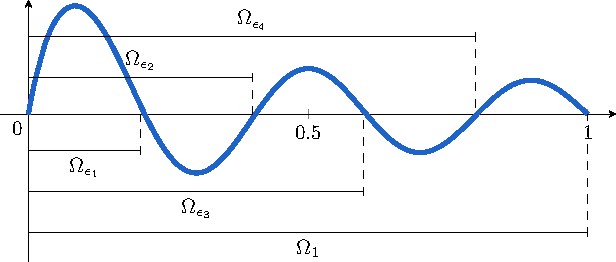
\includegraphics[width=.9\textwidth]{img/chapter3/counting/sturm-liouville.pdf}
    \caption{Eigenfunction $y_4$, with $\lambda_4 \approx 246.74$, of the $\nicefrac{1}{2}$-order Bessel equation~\cite{titchmarsh_eigenfunction_1962} $-\dv{x}{} \left( x \dv{y}{x} \right) + \frac{1}{4x} y = \lambda x y $ on $[0, 1]$, with $y(0) = y(1) = 0$. The four subintervals, $\Omega_{\epsilon_1} = [0, \epsilon_1],\dots, \Omega_{\epsilon_4} = [0, \epsilon_4]$, on which $\lambda_4$ is also an eigenvalue of this equation, are indicated.}\label{fig:c3_counting_sturm_liouville}
  \end{center}
\end{figure}

Multiple shooting procedures~\cite{baeyens_fast_2020,ledoux_matslise_2016,ixaru_cp_2000} have been developed that implement this well-known property for Sturm--Liouville problems using the Prüfer transformation~\cite{pruefer_neue_1926}.

\subsubsection{Standing waves on a disc}\label{sec:c3_standing_waves_on_disc}

Consider the eigenvalues and eigenfunctions of the two-dimensional wave equation
\begin{equation}\label{equ:c3_disc_before_polar}
  -\nabla^2 \psi(x, y) = \lambda \psi(x, y)
\end{equation}
on the unit disc with homogeneous Dirichlet boundary condition.

In many introductory textbooks to (partial) differential equations, the study of the wave equation on a drum is considered. In most texts, if not all, the idea boils down to: with a transformation into polar coordinates and separation of variables, this two-dimensional problem can be transformed into two one-dimensional problems. One of these can be solved directly, the other gives rise to the so-called Bessel functions.

Here we will give a brief overview of the symbolic calculations to solve~\eqref{equ:c3_disc_before_polar} on the unit disc $B(\vb{0}, 1)$, with homogeneous Dirichlet boundary conditions. For more details one could consult for example~\cite[chapter~4]{asmar_partial_2005}. As stated, we first transform~\eqref{equ:c3_disc_before_polar} to polar coordinates. For this we pose $x = r\cos(\theta)$ and $y = r\sin(\theta)$, with $r \in [0,1]$ and $\theta \in [0, 2\pi]$. The solutions $u(r, \theta) := \psi(r\cos(\theta), r\sin(\theta))$ are now considered in the transformed domain. Applying the chain rule to $\nabla^2\psi$ yields the new equation
\begin{equation}\label{equ:c3_disc_after_polar}
  -{\pdv[2]{u}{r}} - \frac{1}{r}{\pdv[]{u}{r}} - \frac{1}{r^2} {\pdv[2]{u}{\theta}} = - \lambda u\text{.}
\end{equation}
The boundary conditions are likewise transformed: $u(1, \theta) = 0$ for all $\theta \in [0, 2\pi]$ and $u(r, 0) = u(r, 2\pi)$ and ${\pdv[]{u}{\theta}}(r, 0) = {\pdv[]{u}{\theta}}(r, 2\pi)$ for all $r \in [0, 1]$.

Now we use the method of separation of variables to transform~\eqref{equ:c3_disc_after_polar} into two one-dimensional problems. For this, we separate $u(r, \theta) = R(r) \Theta(\theta)$ into a product of an $r$-dependent function and a $\theta$-dependent function. This allows us to write
$$
  -\frac{r^2 R''}{R} - \frac{rR'}{R} - \frac{\Theta''}{\Theta} = \lambda r^2 \text{.}
$$
Rearranging terms to an $r$-dependent side and a $\theta$-dependent side yields two separate equations
\begin{align*}
  \lambda r^2 + \frac{r^2 R''}{R} + \frac{rR'}{R} & = k & \text{and} &  & -\frac{\Theta''}{\Theta} & = k\text{,}
\end{align*}
with $k$ a constant and boundary conditions $R(1) = 0$, $\Theta(0) = \Theta(2\pi)$ and $\Theta'(0) = \Theta'(2\pi)$.

Solutions for $\Theta(\theta)$ can directly be found as a solution of a linear second order differential equation with constant coefficients. Thus, $\Theta$ only has periodic solutions
$$
  \Theta(\theta) = A_m \cos(m\theta) + B_m \sin(m\theta)\text{,}
$$
if $k = m^2$ with $m \in \{0, 1, 2, \dots\}$. Note that if $m > 0$, there are two linear independent solutions for $\Theta$.

The differential equation for $R(r)$ becomes
$$
  r^2 R'' + r R + (\lambda r^2 - m^2)R = 0\text{.}
$$
We find that solutions to our equation can be written using the $m^\text{th}$ Bessel function of the first kind $R(r) = J_m(r \sqrt{\lambda})$, for more details about these functions see for example~\cite[section~4.7]{asmar_partial_2005}. These solutions only satisfy the boundary condition $R(1) = 0$ if and only if $\sqrt{\lambda}$ is a positive zero of $J_m$. If we denote $j_{m, n}$ as the $n^\text{th}$ positive root of the $m^\text{th}$ Bessel function $J_m$, we find that all eigenvalues of~\eqref{equ:c3_disc_after_polar}, and also of~\eqref{equ:c3_disc_before_polar}, are given as the squares of roots of the Bessel functions. So $\lambda = j_{m, n}^2$ is an eigenvalue of~\eqref{equ:c3_disc_before_polar}. It is a single eigenvalue if $m = 0$, otherwise it is a double eigenvalue. The following table contains the first ten eigenvalues, counted with multiplicity.

\begin{center}
  \bgroup
  \def\arraystretch{1.5}
  \begin{tabular}{r|cccccc}
    Eigenvalue       & $\lambda_0$ & $\lambda_{1,2}$ & $\lambda_{3,4}$ & $\lambda_{5}$ & $\lambda_{6,7}$ & $\lambda_{8,9}$ \\ \hline\hline
    Analytical value & $j_{0,1}^2$ & $j_{1,1}^2$     & $j_{2,1}^2$     & $j_{0,2}^2$   & $j_{3,1}^2$     & $j_{1,2}^2$     \\ \hline
    Numerical value  & $5.783$     & $14.68$         & $26.37$         & $30.47$       & $40.71$         & $49.22$
  \end{tabular}
  \egroup
\end{center}

To apply theorem~\ref{the:c3_counting_eigenvalues} we need to define a family of domains. A most obvious choice would be all concentric discs with radius at most one. With a variable substitution we know the eigenvalues of the wave equation on $\Omega_\epsilon := B(\vb{0}, \epsilon)$ to be $\frac{\lambda_{i}}{\epsilon^2}$ for all eigenvalues $\lambda_{i}$ on the unit disc. It is obvious that the eigenvalues $\frac{\lambda_{i}}{\epsilon^2}$ as a function of $\epsilon$, are continuous, decreasing, and unbounded as $\epsilon \to 0^{+}$. This confirms lemma~\ref{lem:c3_eigenvalues_curves}.

Concentric discs may not be the most thrilling examples. But in the example in section~\ref{sec:c3_counting_exotic_domain} we will consider a much more interesting family of domains for the wave equation on a disc.

\subsubsection{A two-dimensional Schrödinger equation}\label{sec:c3_counting_ixaru}

In this example, we will take a look at a two-dimensional time-independent Schrödinger equation with homogeneous Dirichlet boundary conditions on a rectangle:
$$
  -\nabla^2 \psi + V(x, y)\psi = E\psi\text{.}
$$

In section~\ref{sec:c3_experiment_ixaru}, we will study the Schrödinger problem with the potential
$$
  V(x, y) = (1+x^2)(1+y^2)
$$
on the square $[-5.5; 5.5] \times [-5.5; 5.5]$ with homogeneous Dirichlet boundary conditions. The first eigenvalues are reported in~\cite{ixaru_new_2010} to be as follows.

\begin{center}
  \begin{tabular}{r|n{1}{7}cr|n{2}{7}}
    $E_{0}$         & 3.1959181 & \hspace*{2cm} & $E_{6} = E_{7}$ & 9.9280611  \\
    $E_{1} = E_{2}$ & 5.5267439 &               & $E_{8} = E_{9}$ & 11.3118171 \\
    $E_{3}$         & 7.5578033 &               & $E_{10}$        & 12.1032536 \\
    $E_{4}$         & 8.0312723 &               & $E_{11}$        & 12.2011790 \\
    $E_{5}$         & 8.4445814 &               & $E_{12}$        & 13.3323313
  \end{tabular}
\end{center}

For this problem we will use the method as described in section~\ref{sec:c3_ixarus_method}. In summary, this is a shooting method, which means that it guesses a value for $E$ and calculates a matching error. This matching error is then used to improve the estimation of $E$. This process is repeated until $E$ is found up to the desired accuracy.

By propagating all possible eigenfunctions $u(x, y)$ from the bottom and the top of the domain to the matching line, this matching error is calculated. In the context of theorem~\ref{the:c3_counting_eigenvalues}, this propagation can be thought of as going through all possible subdomains from figure~\ref{fig:intuitive_example_rho}. If, while propagating, any of the possible eigenfunctions $u$ becomes identically zero on a line, then a subdomain is found on which $E$ is an eigenvalue.

\begin{figure}
  \begin{center}
    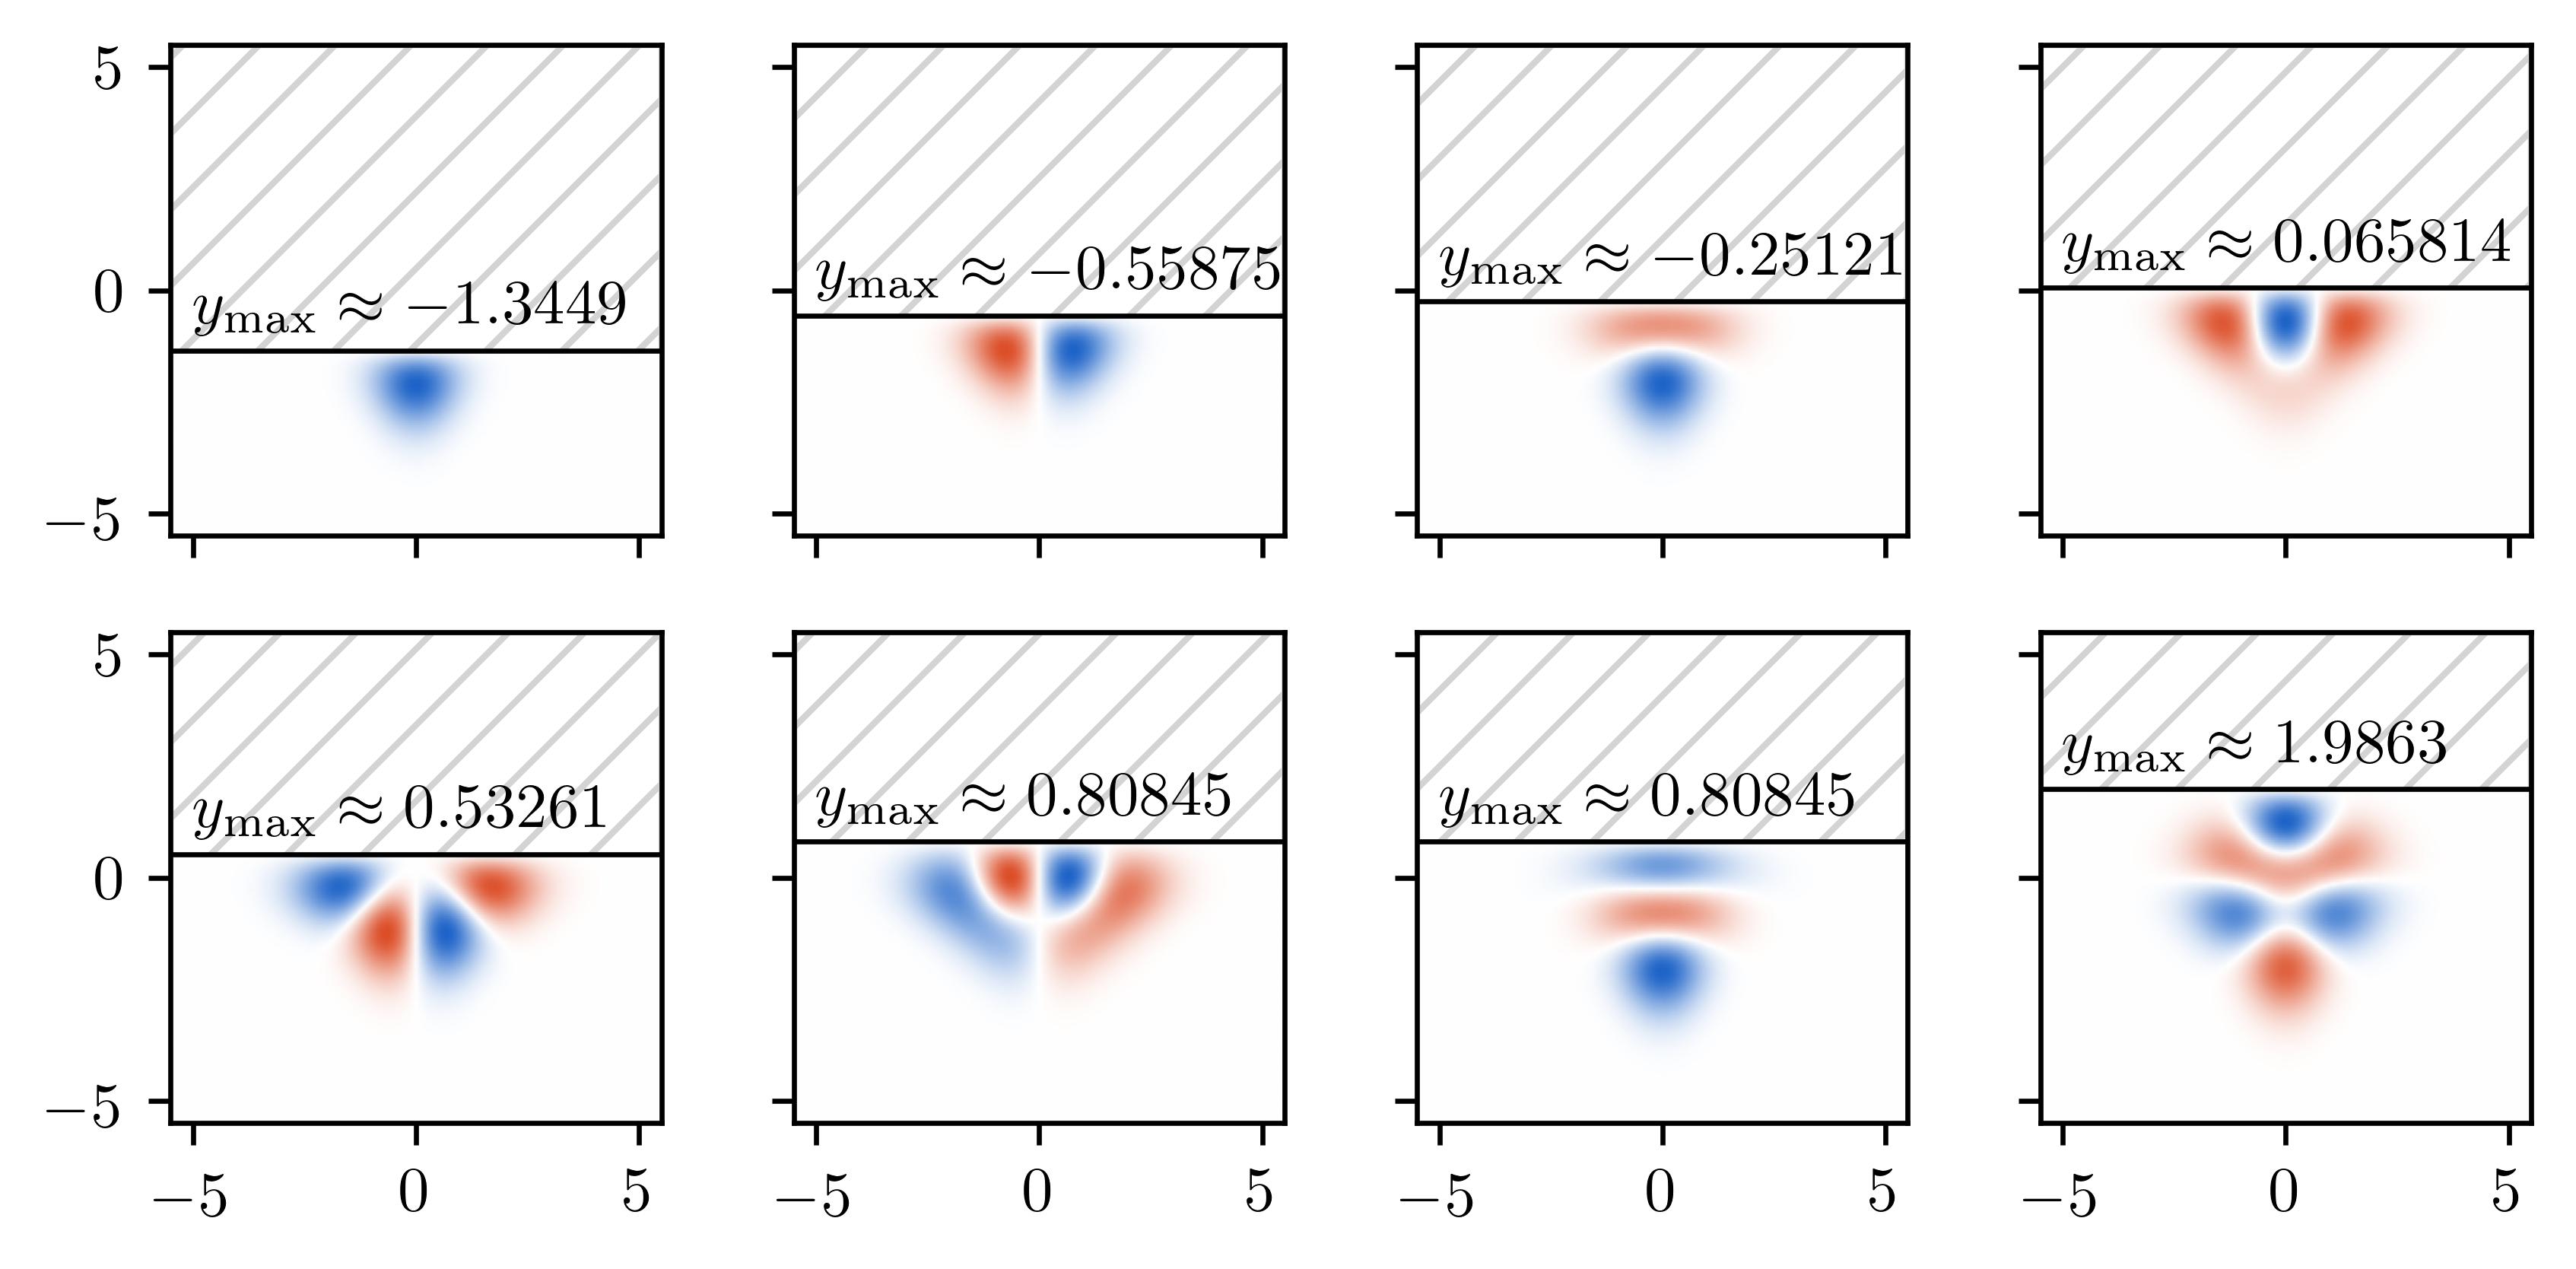
\includegraphics[width=1\textwidth]{img/chapter3/counting/ixaru.png}
  \end{center}
  \caption{There are 8 (smaller) rectangles on which $E = 11$ is an eigenvalue of the Schrödinger problem from example~\ref{sec:c3_counting_ixaru}.}\label{fig:c3_counting_ixaru_subdomains}
  \vspace{1cm}
  \begin{center}
    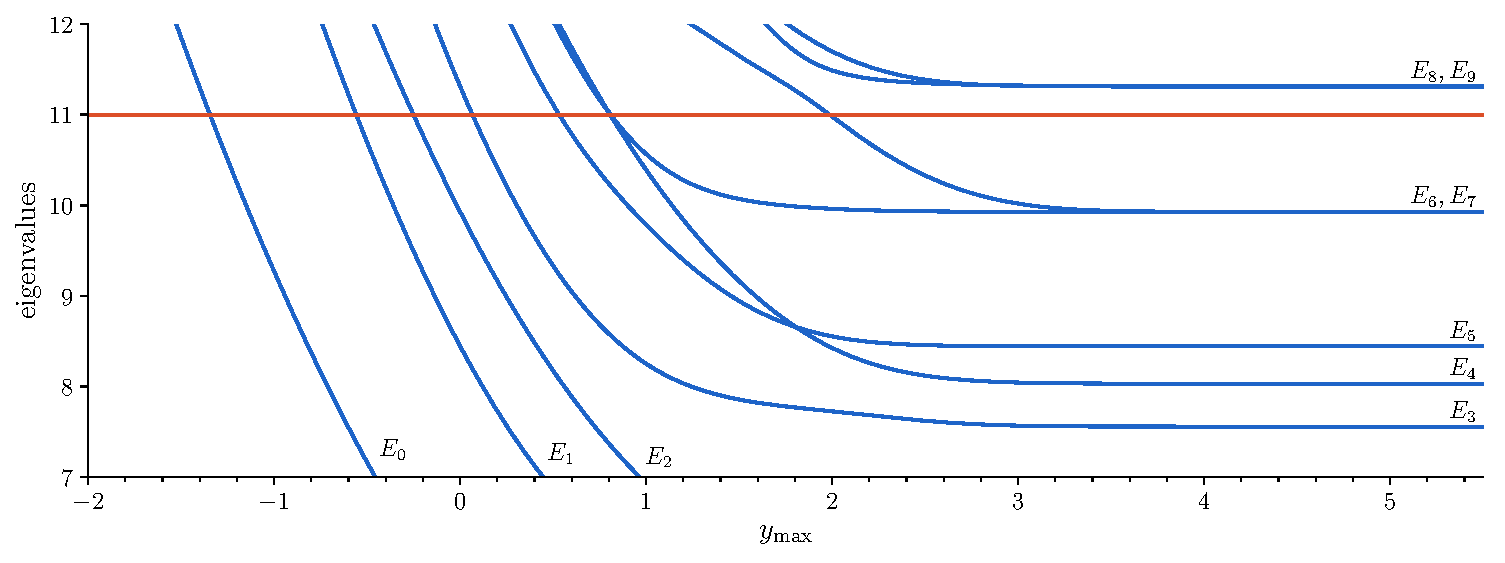
\includegraphics[width=1\textwidth]{img/chapter3/counting/counting_eigenvalues_zoom.pdf}
  \end{center}
  \caption{Here, a zoomed in version of figure~\ref{fig:c3_counting_eigenvalue_graph} is displayed. Each blue graph represents an eigenvalue of the Schrödinger equation from example~\ref{sec:c3_counting_ixaru}. The fixed line $E = 11$ is represented in red. Each crossing of the red line and a blue graph represents a smaller subdomain on which $E=11$ is an eigenvalue. These subdomains, with corresponding eigenfunction, are illustrated in figure~\ref{fig:c3_counting_ixaru_subdomains}.}\label{fig:counting_eigenvalues_zoom}
\end{figure}

For each $E$, while propagating, one can keep track of how many $u$ did become zero on a line, or in other words, on how many subdomains $E$ is an eigenvalue. Following theorem~\ref{the:c3_counting_eigenvalues}, this number tells us how many eigenvalues there are less than $E$ on the whole domain. In figure~\ref{fig:c3_counting_ixaru_subdomains}, keeping track of when an eigenfunction becomes zero on a line is demonstrated. For $E = 11$, all domains are visualized where any $u(x, y) = 0$ for all $x \in [\xmin, \xmin]$. Notice that there may be domains on which multiple eigenfunctions are found for that particular value of $E$. These domains should be counted multiple times. In figure~\ref{fig:c3_counting_ixaru_subdomains}, we see that $\ymax \approx \numprint{0.80845}$ is counted twice. From the tabulated true eigenvalues in~\cite{ixaru_new_2010}, we know that there are indeed exactly $8$ eigenvalues less than $E = 11$. This example thus verifies theorem~\ref{the:c3_counting_eigenvalues} as well.

For completeness, we will also verify lemma~\ref{lem:c3_eigenvalues_curves} by taking a closer look at the graph from figure~\ref{fig:c3_counting_eigenvalue_graph}. In figure~\ref{fig:counting_eigenvalues_zoom} we see a zoomed version. These graphs describe how the eigenvalues evolve through the growing domain. If we draw a horizontal line at $E = 11$, as in figure~\ref{fig:counting_eigenvalues_zoom}, eight curves intersect this line. Each curve corresponds to a lower lying eigenvalue, just as lemma~\ref{lem:c3_eigenvalues_curves} predicts.


\subsubsection{A more exotic family of domains}\label{sec:c3_counting_exotic_domain}

\begin{figure}
  \begin{center}
    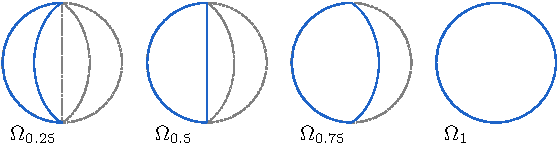
\includegraphics[width=\linewidth]{img/chapter3/counting/moons.pdf}
    \caption{An illustration of the family of domains we consider in section~\ref{sec:c3_counting_exotic_domain}.}\label{fig:c3_counting_visual_moons}
  \end{center}
\end{figure}

As a numerical demonstration for theorem~\ref{the:c3_counting_eigenvalues} with less trivial domains, we consider the wave equation on a series of moon-shaped domains with homogeneous Dirichlet boundary conditions. Visually, these domains can be found in figure~\ref{fig:c3_counting_visual_moons}. Mathematically, we define the transformation $T:[-\frac{\pi}{2}, \frac{\pi}{2}] \times [-1, 1] \to \RR^2$ as:
\begin{equation}\label{equ:c3_disc_transformation}
  T(\alpha, t) = \begin{pmatrix}
    \cot(\alpha) \sin(t \alpha) \\
    \frac{1}{\sin(\alpha)} - \cot(\alpha) \cos(t \alpha)
  \end{pmatrix}\text{.}
\end{equation}
Strictly speaking, for $\alpha = 0$,  $T(\alpha, t)$ is undefined. In these points, the limit $\lim_{\alpha \to 0} T(\alpha, t)$ should be considered. In figure~\ref{fig:c3_disc_transformation}, this transformation is visualized. Note that when $t$ is limited to $[-1, 2\epsilon -1]$ the transformation results in a moon-shape.

\begin{figure}
  \begin{center}
    \begin{minipage}{.53\textwidth}
      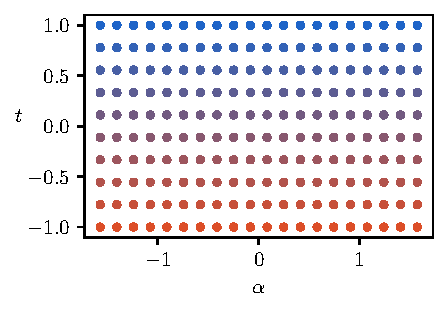
\includegraphics[scale=.75]{img/chapter3/on_disc/disc_original.pdf}%
    \end{minipage}\begin{minipage}{.05\textwidth}\begin{center}
        \Large $ \xrightarrow{T} $
      \end{center}
    \end{minipage}\begin{minipage}{.42\textwidth}\centering
      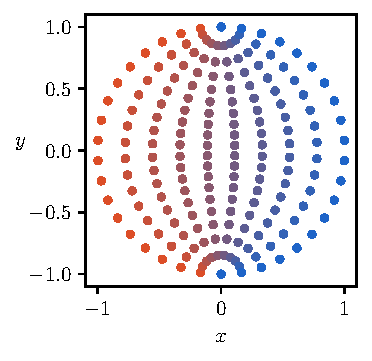
\includegraphics[scale=.75]{img/chapter3/on_disc/disc_transformed.pdf}
    \end{minipage}
  \end{center}
  \caption{The transformation $T(\alpha, t)$ from~\eqref{equ:c3_disc_transformation} is applied to a grid of points.}
  \label{fig:c3_disc_transformation}
\end{figure}

To illustrate the applicability of theorem~\ref{lem:c3_eigenvalues_curves}, we will consider the family of continuous subdomains
$$
  \Omega_\epsilon = \left\{T(\alpha, t) \,\middle|\, \forall \alpha \in \left[-\frac{\pi}{2}, \frac{\pi}{2}\right], \forall t \in [-1, 2\epsilon - 1]  \right\}\text{.}
$$
On each of these subdomains $\Omega_\epsilon$, we will approximate the eigenvalues of the Schrödinger equation with zero potential:
\begin{equation}\label{equ:c3_disc_schrodinger}
  -\nabla^2 \psi(x, y) = \lambda \psi(x, y)\text{.}
\end{equation}
As a boundary condition we impose $\psi(x, y) = 0$ on the boundary $\dOmega_\epsilon$.

Later on, the approximate eigenvalues found can be compared to the eigenvalues on the unit disc $\Omega_1$, as described in section~\ref{sec:c3_standing_waves_on_disc}. Theorem~\ref{the:c3_counting_eigenvalues} promises that, for an eigenvalue $\lambda_i$ on the unit disc, exactly $i$ moon-shaped subdomains can be found on which this $\lambda_i$ is also an eigenvalue.

\paragraph{Transforming the problem onto a rectangular domain}

Approximating solutions for the eigenvalues of~\eqref{equ:c3_disc_schrodinger} on such an exotic domain $\Omega_\epsilon$ is not a trivial task. In principle, this problem could be seen as solving the Schrödinger equation on $[-1,1]^2$ with the potential
$$
  V(x, y) = \begin{cases}
    0       & \text{if $(x, y)\in \Omega_\epsilon$} \\
    +\infty & \text{otherwise.}
  \end{cases}
$$
Numerically, this does not make the problem easier. On the one hand, the rectangular domain would allow us to employ the earlier developed method. On the other hand however, the potential becomes infinite, which is very difficult to implement with sufficiently high accuracies. Also, Ixaru's two-dimensional method has difficulties with non-continuous potentials. Note that the inability to tackle non-continuous problems is a phenomenon present in many high-order numerical methods. In section~\ref{sec:c2_experiment_with_jumps}, we have seen that with one-dimensional problems, \matslise{} can avoid these issues by smartly choosing its piecewise approximation. For higher-dimensional problems, these kinds of tricks are no longer possible.

We propose another technique. We can transform equation~\eqref{equ:c3_disc_schrodinger} from these moon-shaped domains to a more manageable rectangular domain. The cost of this transformation is that~\eqref{equ:c3_disc_schrodinger} will no longer be a Schrödinger equation.

As stated earlier, the transformation we will apply is the function $(x, y) = T(\alpha, t)$ from~\eqref{equ:c3_disc_transformation}. To formalize this, we introduce $\phi(\alpha, t)$ as
$$
  \phi(\alpha, t) = \psi(T(\alpha, t))\text{.}
$$
With this transformation, the Schrödinger equation~\eqref{equ:c3_disc_schrodinger} transforms into
\begin{equation}\label{equ:c3_disc_schrodinger_transformed}
  -\mathcal{D}\phi(\alpha, t) = \lambda\phi(\alpha, t)\text{,}
\end{equation}
with $\phi(\alpha, t)$ defined on the domain $\Xi_\epsilon = \left[-\frac{\pi}{2}, \frac{\pi}{2}\right] \times [-1, 2\epsilon - 1]$. Note that $T(\Xi_\epsilon) = \Omega_\epsilon$. As boundary conditions we impose $\phi(\alpha, t) = 0$ if $(\alpha, t) \in \partial\Xi_\epsilon$. In this expression, $\mathcal{D}$ is the differential operator corresponding to $\nabla^2\psi(x, y)$. Calculating this operator by hand is tedious, therefore we will use \sage{} to do the symbolic heavy lifting for us. To be able to work with the operator $\mathcal{D}$, we first need a procedure to compute it. To ease notation, we will denote $T(\alpha, t) = (T^{x}(\alpha, t), T^{y}(\alpha, t))$, and omit the arguments to the functions $\phi$, $\psi$ and $T$. Derivatives will be denoted as $\phi_\alpha = \pdv[]{\phi}{\alpha}$ and $\phi_{\alpha\alpha} = \pdv[2]{\phi}{\alpha}$. We compute all first and second derivatives of $\phi(\alpha, t)$.
\begin{equation}\label{equ:disc_transformation_derivatives}
  \begin{cases}
    \phi_\alpha = \psi_x T^x_\alpha + \psi_y T^y_\alpha                                                                                                                   \\
    \phi_t = \psi_x T^x_t + \psi_y T^y_t                                                                                                                                  \\
    \phi_{\alpha\alpha} = \psi_x T^x_{\alpha\alpha} + \psi_y T^y_{\alpha\alpha} + \psi_{xx} (T^x_\alpha)^2 + 2 \psi_{xy} T^x_\alpha T^y_\alpha + \psi_{yy} (T^y_\alpha)^2 \\
    \phi_{\alpha t} = \psi_x T^x_{\alpha t} + \psi_y T^y_{\alpha t} + \psi_{xx} (T^x_\alpha)(T^x_t) + \psi_{xy} \left(T^x_\alpha T^y_t + T^x_t T^y_\alpha \right)         \\
    \quad\quad\quad\quad {} + \psi_{yy} (T^y_\alpha)(T^y_t)                                                                                                               \\
    \phi_{tt} = \psi_x T^x_{tt} + \psi_y T^y_{tt} + \psi_{xx} (T^x_t)^2 + 2 \psi_{xy} T^x_t T^y_t + \psi_{yy} (T^y_t)^2
  \end{cases}
\end{equation}

The question now is: can we isolate $\psi_{xx} + \psi_{yy}$ from the right-hand side of the system from~\eqref{equ:disc_transformation_derivatives}? As this is a linear system in the derivatives of $\psi$, there is a unique linear combination $\vb{c}(\alpha, t) = (c^\alpha, c^t, c^{\alpha\alpha}, c^{\alpha t}, c^{tt})$ such that:
$$
  c^\alpha \phi_\alpha + c^t\phi_t + c^{\alpha\alpha}\phi_{\alpha\alpha} + c^{\alpha t} \phi_{\alpha t} + c^{tt} \phi_{tt} = \psi_{xx} + \psi_{yy}\text{.}
$$

This linear combination allows us to finally determine the operator $\mathcal{D}$, and by extension, the partial differential equation~\eqref{equ:c3_disc_schrodinger} transforms into. Note that, since $\vb{c}$ is dependent on $\alpha$ and $t$, the operator $\mathcal{D}$ has this dependency as well,
$$
  \mathcal{D} = c^\alpha {\pdv[]{}{\alpha}} + c^t \pdv[]{}{t} + c^{\alpha\alpha} \pdv[]{}{\alpha\alpha} + c^{\alpha t} \pdv[]{}{\alpha t} + c^{tt} \pdv[]{}{tt}\text{.}
$$

\paragraph{A specialized numerical method}

Before we can analyze the eigenvalues of the transformed operator $-\mathcal{D}$ in relation to the domain $\Omega_\epsilon$, we still need a method to approximate these eigenvalues. For general partial differential equations with appropriate boundary conditions, some standard techniques are available.~\cite[Chapter~11]{heath_scientific_2002} contains an overview of some of these methods. Our choices include, but are not limited to, a finite difference method, a finite element method, or a semidiscrete method with shooting. For our purposes, a method that is easy to implement that gives reliable results will be the best choice. A simple finite difference scheme will be sufficient.

We will place an $n_\alpha \times n_t$ grid on the domain $\Xi_\epsilon$. This gives rise to the equidistant points $-\frac{\pi}{2}=\alpha_0, \alpha_1, \dots, \alpha_{n_\alpha} = \frac{\pi}{2}$, and the points $-1 = t_0, t_1, \dots t_{n_t} = -1 + 2\epsilon$. The distances between two points are given by $h_\alpha = \frac{\pi}{n_\alpha}$ and $h_t = \frac{2\epsilon}{n_t}$. Because of the homogeneous Dirichlet boundary conditions $\phi_{0,j} = \phi_{n_\alpha,j} = \phi_{i, 0} = \phi_{i,n_t} = 0$ for all $i$ and $j$. These grid points allow us to write down approximations of the first and second derivatives of $\phi(\alpha, t)$ in each of the grid points $\phi_{i, j} = \phi(\alpha_i, t_j)$.
\begin{align*}
  {\pdv[]{\phi}{\alpha}}(\alpha_i, t_j)    & \approx \frac{1}{2h_\alpha}\left( \phi_{i+1,j} - \phi_{i-1,j} \right)                                           \\
  {\pdv[]{\phi}{t}}(\alpha_i, t_j)         & \approx \frac{1}{2h_t}\left( \phi_{i,j+1} - \phi_{i,j-1} \right)                                                \\
  {\pdv[2]{\phi}{\alpha}}(\alpha_i, t_j)   & \approx \frac{1}{h_\alpha^2}\left( \phi_{i+1,j} - 2 \phi_{i,j} + \phi_{i-1,j} \right)                           \\
  {\pdv[]{\phi}{\alpha}{t}}(\alpha_i, t_j) & \approx \frac{1}{4h_\alpha h_t}\left( \phi_{i+1,j+1} - \phi_{i+1,j-1} - \phi_{i-1,j+1} + \phi_{i-1,j-1} \right) \\
  {\pdv[2]{\phi}{t}}(\alpha_i, t_j)        & \approx \frac{1}{h_t^2}\left( \phi_{i,j+1} - 2 \phi_{i,j} + \phi_{i,j-1} \right)\text{.}
\end{align*}

When working with finite difference schemes, especially for a more  advanced operator such as $\mathcal{D}$, writing out all formulae becomes quite tedious. Therefore, it is much more comprehensive if we introduce some matrix notation. Let us denote $\vb{I}_n$ as the $n \times n$ identity matrix. Furthermore, a diagonal matrix with $a_1, \dots, a_n$ on the diagonal will be denoted as $\diag_n(a_1, \dots, a_n)$, and an $n \times n$ tridiagonal Toeplitz matrix, with $c_{0}$ on the main diagonal, $c_{-1}$ below it and $c_1$ above it, will be denoted as $\tridiag_{n}(c_{-1}, c_{0}, c_1)$. To aid the notation of the finite difference approximations we introduce $\vb{D}^{(1)}_n = \frac{1}{2}\tridiag_n(-1,0,1)$ and $\vb{D}^{(2)}_n = \tridiag_n(1,-2,1)$.

The Kronecker product of a $k \times l$ matrix $\vb{A}$ and an $m \times n$ matrix $\vb{B}$ is defined as the $km \times ln$ block matrix:
$$
  \vb{A} \otimes \vb{B} := \begin{pmatrix}
    A_{1,1} \vb{B} & A_{1, 2} \vb{B} & \dots  & A_{1, l} \vb{B} \\
    A_{2,1} \vb{B} & A_{2, 2} \vb{B} & \dots  & A_{2, l} \vb{B} \\
    \vdots         & \vdots          & \ddots & \vdots          \\
    A_{k,1} \vb{B} & A_{k, 2} \vb{B} & \dots  & A_{k, l} \vb{B}
  \end{pmatrix}{}\text{.}
$$

To approximate~\eqref{equ:c3_disc_schrodinger_transformed} as a matrix problem, we need to aggregate the grid points $\phi_{i,j}$ as a vector. For this we define
$$
  \vb*{\phi} := \transpose{\begin{pmatrix}
      \phi_{1,1} & \phi_{2,1} & \dots & \phi_{n_\alpha-1, 1} & \phi_{1,2} & \dots & \phi_{n_\alpha-1, n_t-1}
    \end{pmatrix}}\text{.}
$$
Also, to be able to write down $\mathcal{D}$ as a matrix operation, we need to define
$$
  \vb{C}^{t} := \diag\left(
      c^{t}(\alpha_1, t_1) , \dots , c^{t}(\alpha_{n_\alpha-1}, t_1) , c^{t}(\alpha_1, t_2) , \dots , c^{t}(\alpha_{n_\alpha-1}, t_{n_t-1})
    \right)\text{,}
$$
and analogously for $\vb{C}^{\alpha}$, $\vb{C}^{\alpha\alpha}$, $\vb{C}^{\alpha t}$ and $\vb{C}^{t t}$.

All these notations allow us to approximate~\eqref{equ:c3_disc_schrodinger_transformed} as a matrix eigenvalue problem:
$$
  -\vb{M} \vb*{\phi} = \lambda \vb*{\phi}
$$
with
\begin{align*}
  \vb{M} = {} & \frac{1}{h_\alpha} \vb{C}^{\alpha} \left(\vb{I}_{n_t - 1}\otimes \vb{D}^{(1)}_{n_\alpha - 1} \right) + \frac{1}{h_t} \vb{C}^{t} \left(\vb{D}^{(1)}_{n_t - 1}  \otimes \vb{I}_{n_\alpha - 1}\right)                \\
              & {} + \frac{1}{h_\alpha^2} \vb{C}^{\alpha\alpha} \left(\vb{I}_{n_t - 1}\otimes \vb{D}^{(2)}_{n_\alpha - 1}\right) + \frac{1}{h_t^2} \vb{C}^{tt} \left(\vb{D}^{(2)}_{n_t - 1}  \otimes \vb{I}_{n_\alpha - 1}\right) \\
              & {} + \frac{1}{h_\alpha h_t} \vb{C}^{\alpha t} \left(\vb{I}_{n_t - 1}\otimes \vb{D}^{(1)}_{n_\alpha - 1} \right) \left( \vb{D}^{(1)}_{n_t - 1}  \otimes \vb{I}_{n_\alpha - 1} \right)\text{.}
\end{align*}

\begin{figure}
  \begin{center}
    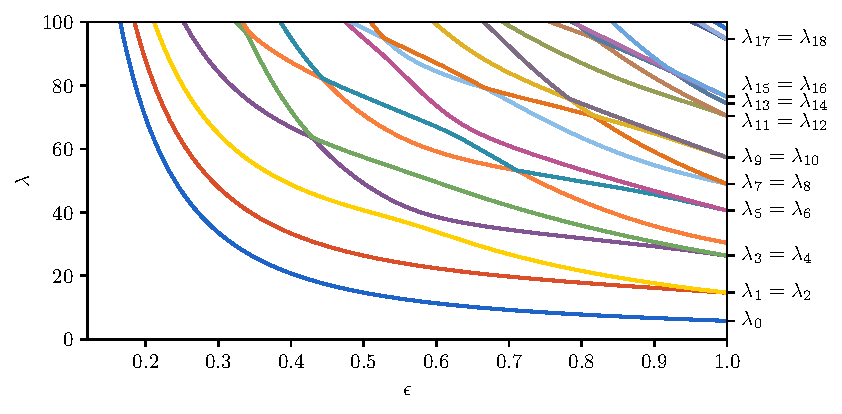
\includegraphics[width=\textwidth]{img/chapter3/on_disc/eigenvalues_flow.pdf}
    \caption{Eigenvalues of the Schrödinger equation with zero potential on the family of domains of section~\ref{sec:c3_counting_exotic_domain} in relation to $\epsilon$.}
    \label{fig:c3_disc_eigenvalues_flow}
  \end{center}
\end{figure}

\paragraph{Analysis of eigenvalues in relation to the domain}

With a numerical method to compute eigenvalues of the wave equation~\eqref{equ:c3_disc_schrodinger} on moon-shaped domains $\Omega_\epsilon$, and a comprehensive analysis of the true eigenvalues of this equation on the disc $\Omega_1$, we are able to illustrate theorem~\ref{lem:c3_eigenvalues_curves}.

By employing our numerical method on different domains $\Omega_\epsilon$, we can construct figure~\ref{fig:c3_disc_eigenvalues_flow}. This figure was computed with $n_\alpha = n_t = 61$ (which makes $\vb{M}$ a $3600\times3600$ sparse matrix) for $200$ equidistantly-spaced values for $\epsilon$. Here, each line corresponds to a different eigenvalue. The lowest blue line visualizes the changes in the lowest eigenvalue according to the domain. For small domains $\epsilon \to 0$, this value becomes larger. The red line right above the blue line corresponds to the eigenvalue with index $1$ of the wave equation on $\Omega_\epsilon$. For $\Omega_1$, this eigenvalue has a double multiplicity $\lambda_1 = \lambda_2$. But for all smaller domains, this degeneracy disappears, and $\lambda_1$ is a single eigenvalue. Which eigenvalue each line represents is marked on the right side. In accordance with theorem~\ref{lem:c3_eigenvalues_curves}, all lines in figure~\ref{fig:c3_disc_eigenvalues_flow} are continuous, decreasing and unbounded when $\epsilon \to 0$.


\begin{figure}
  \begin{center}
    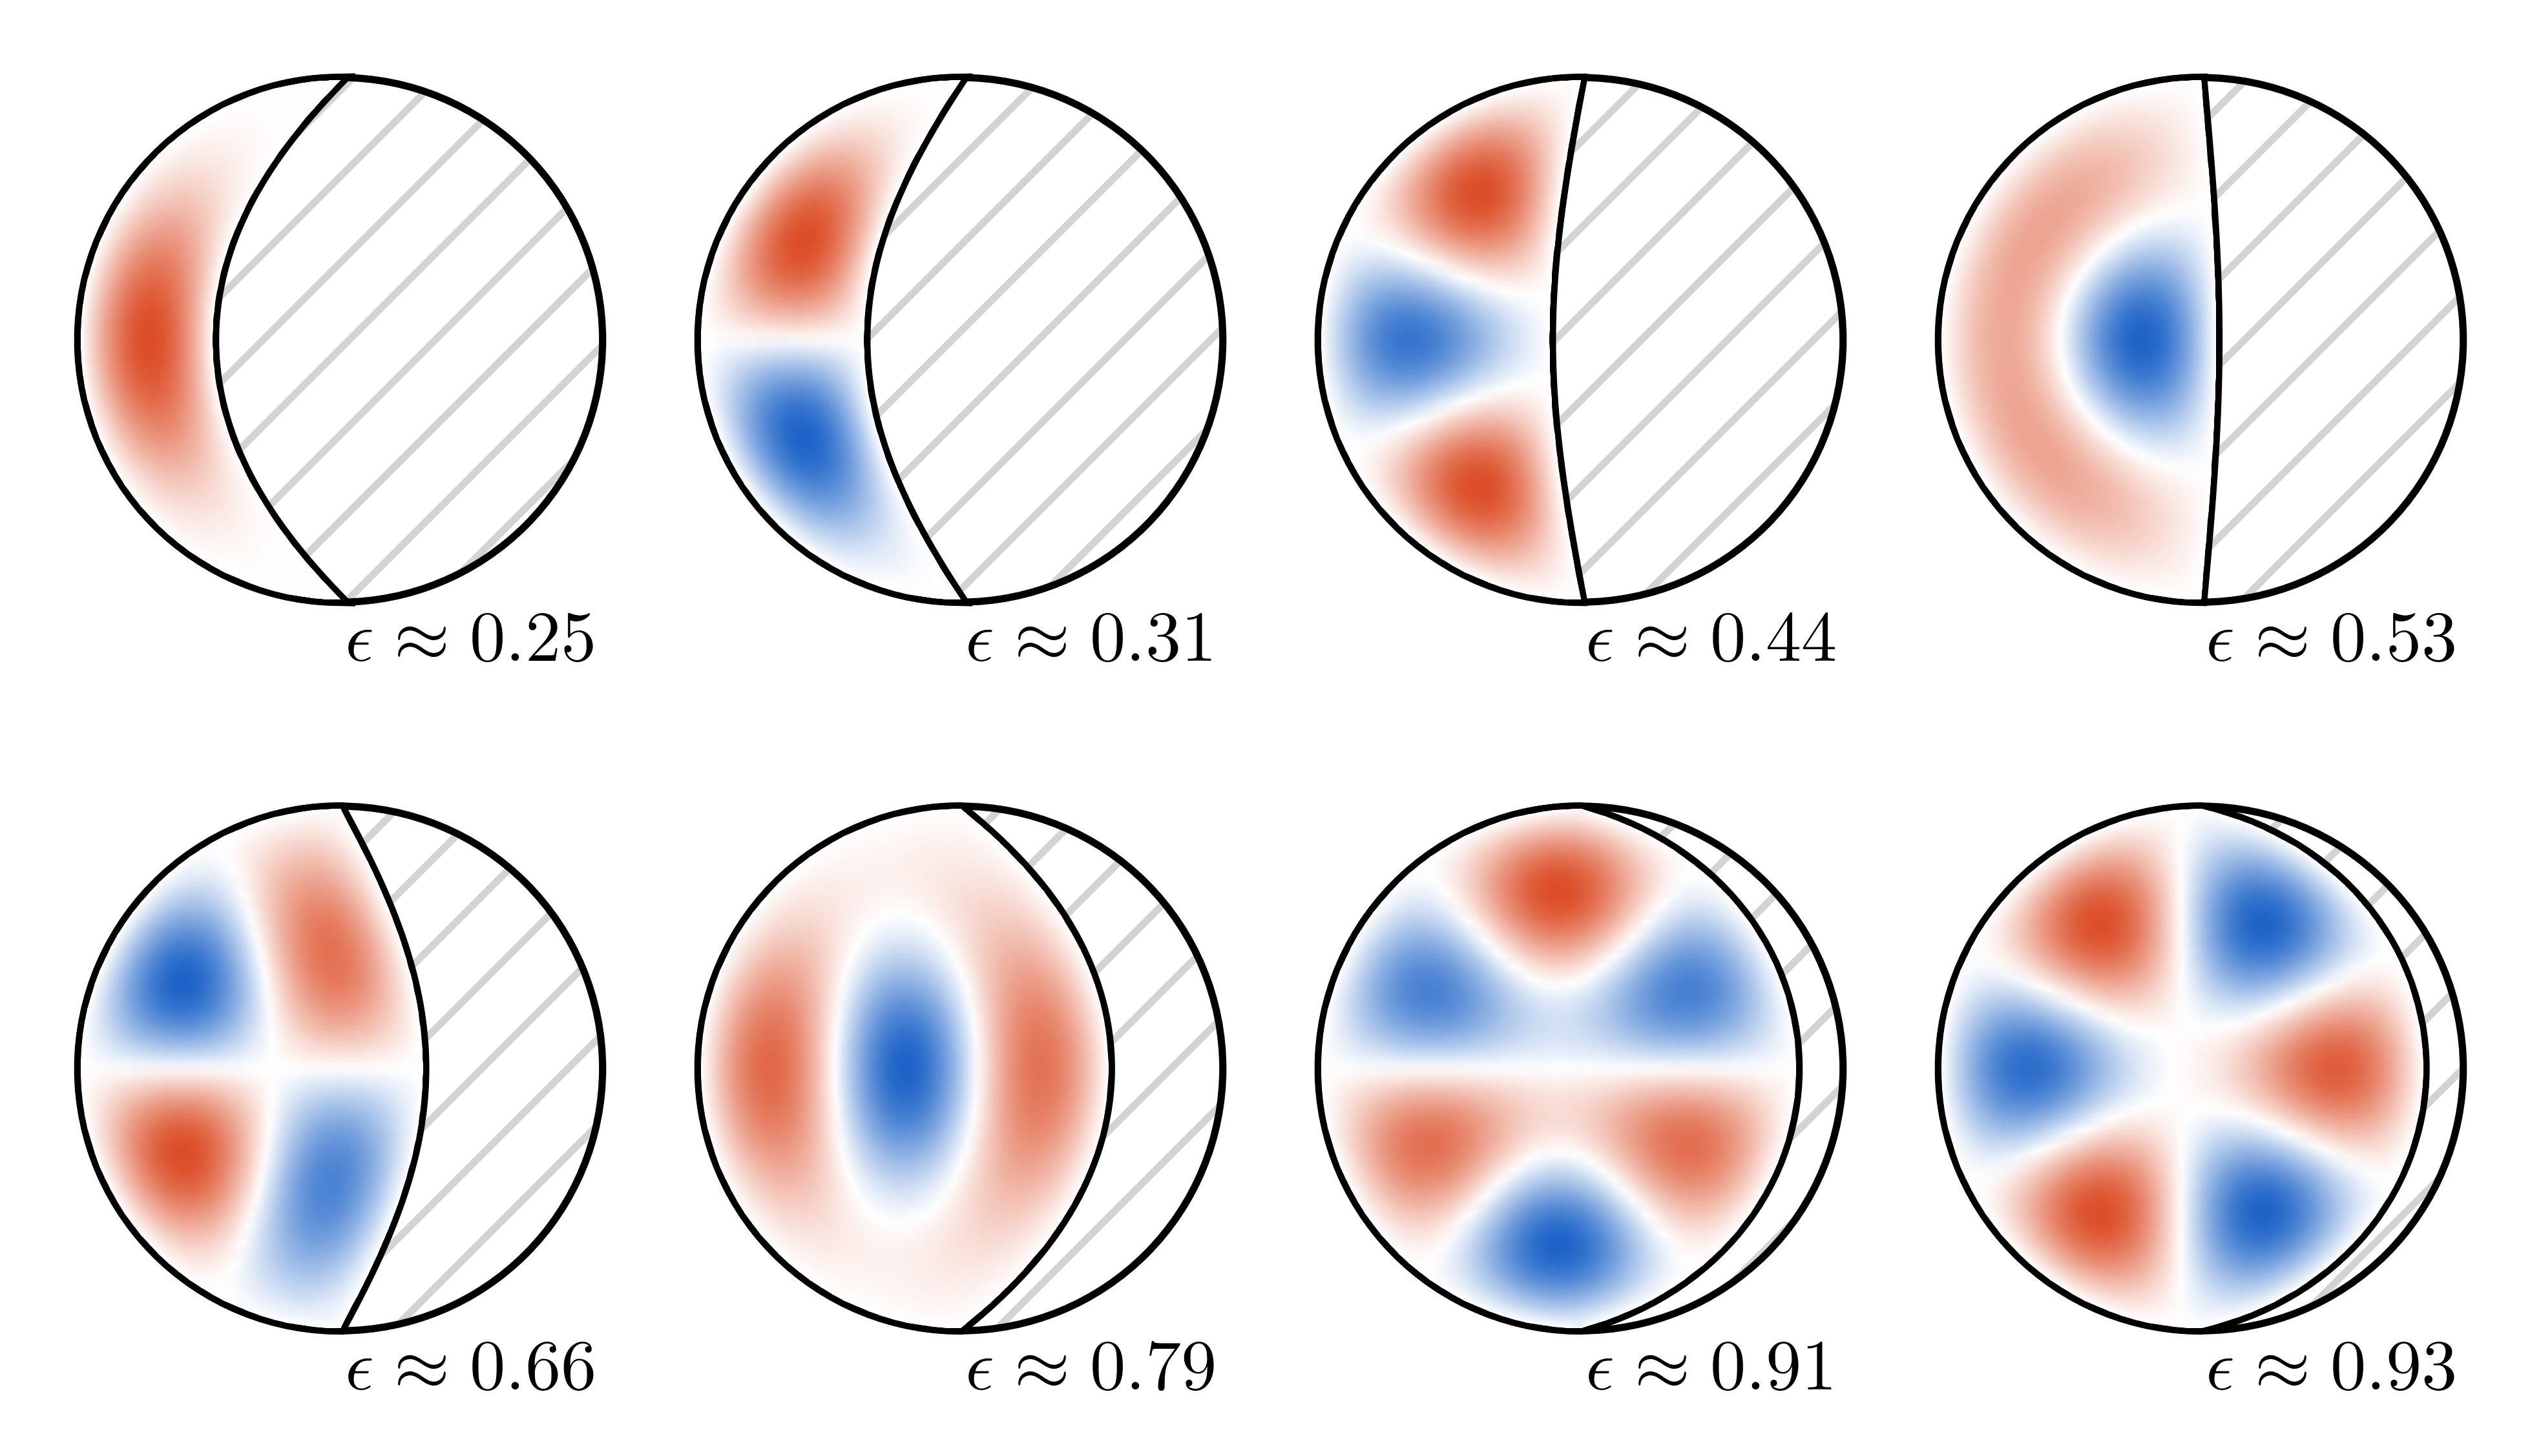
\includegraphics[width=\textwidth]{img/chapter3/on_disc/solutions.png}
    \caption{There are eight smaller moon-shaped domains on which $\lambda = 45$ is an eigenvalue of the wave equation $-\nabla^2 \psi = \lambda \psi$ with homogeneous Dirichlet boundary conditions.}
    \label{fig:c3_disc_solutions}
  \end{center}
\end{figure}


Consider now the fixed value of $E = 45$. From the analysis in~\ref{sec:c3_standing_waves_on_disc} we know that there are eight eigenvalues, counted with multiplicity, less than $E$. This means that, following theorem~\ref{the:c3_counting_eigenvalues}, there should be exactly eight moon-shaped domains on which $E$ is also an eigenvalue. These eight domains, with the corresponding eigenfunction of $E = 45$, are plotted in figure~\ref{fig:c3_disc_solutions}.

\section{Numerical experiments}\label{sec:c3_experiments}

In the previous section, we have made some theoretical advancements. To demonstrate the relevance and effectiveness of the provided theory, we proudly present some numerical results. In summary, the obtained results are at least as accurate as the original method in~\cite{ixaru_new_2010}, but they are found significantly quicker, even when corrected for the more powerful modern CPUs.

Another large improvement can be found in the `autonomy' of the algorithm. In~\cite{ixaru_new_2010}, results for different steps sizes are tabulated. Since we implemented automatic step size selection, this distinction is no longer relevant. To demonstrate that our improvements facilitate using this method, we will also provide some \lpython{}-code. The example code makes use of the package \pyslisetd{}. This package contains our implementation (in \cpp{}, see the discussion from section~\ref{sec:c2_implementation_challenges}) of the earlier described algorithm, together with our improvements.

Via \texttt{pip}, the package \pyslisetd{} can be installed.
% \begin{noindent}
\begin{minted}{bash}
pip install pyslise2d
\end{minted}
% \end{noindent}

\subsection{The zero potential}\label{sec:c3_experiments_zero}

As a first example we will find eigenvalues of the Schrödinger equation with a zero potential
$$
  -\nabla \psi(x, y) = \lambda \psi(x, y)
$$
on the domain $[0, \pi] \times [0, \pi]$ with homogeneous Dirichlet boundary conditions.

In section~\ref{sec:c3_first_example}, we have calculated the eigenvalues to be of the form $i^2 + j^2$ for any $i, j \in \NN^+$, and the corresponding eigenfunction is given by $ \psi(x, y) = \sin(ix)\sin(jy)$. To reiterate, the first few eigenvalues are
$$
  2, 5, 5, 8, 10, 10, 13, 13, 17, 17, 18, 20, 20, 25, 25, 26, 26, 29, 29, 32, \dots
$$

\begin{figure}
  \begin{center}
    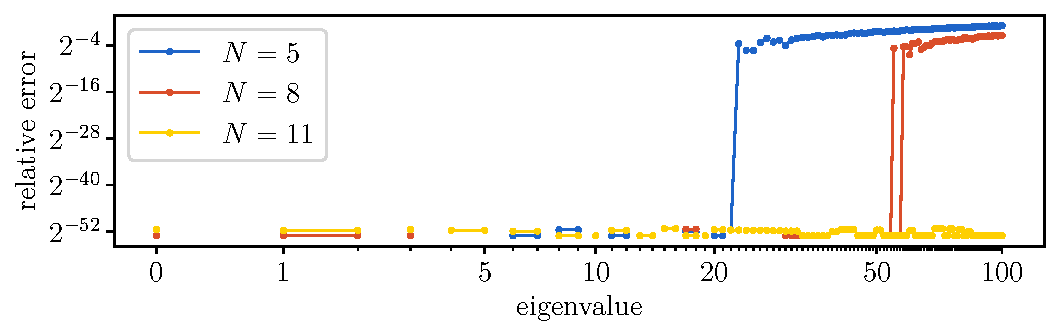
\includegraphics[width=\textwidth]{img/chapter3/experiments/zero.pdf}
  \end{center}
  \caption{The relative error for the first hundred eigenvalues of the zero potential Schrödinger problem on the square $[0, \pi] \times [0, \pi]$ with homogeneous Dirichlet boundary conditions. Degenerate eigenvalues are connected. If a color seems missing for a value, it coincides with another drawn point.}\label{fig:c3_experiment_zero}
\end{figure}

Despite this being the easiest Schrödinger problem to consider, it is non-trivial in the sense that the multiplicity of an eigenvalue is rather unpredictable.

In figure~\ref{fig:c3_experiment_zero}, the relative errors of the first hundred eigenvalues found with \pyslisetd{} are presented. Even for an extremely low number of basis functions used on each sector ($N = 5$), we are still able to reach the most accurate results possible for the first two dozen eigenvalues. However, once the index of the eigenvalue is sufficiently high, the relative error jumps to a value close to $1$.

\begin{figure}
  \begin{center}
    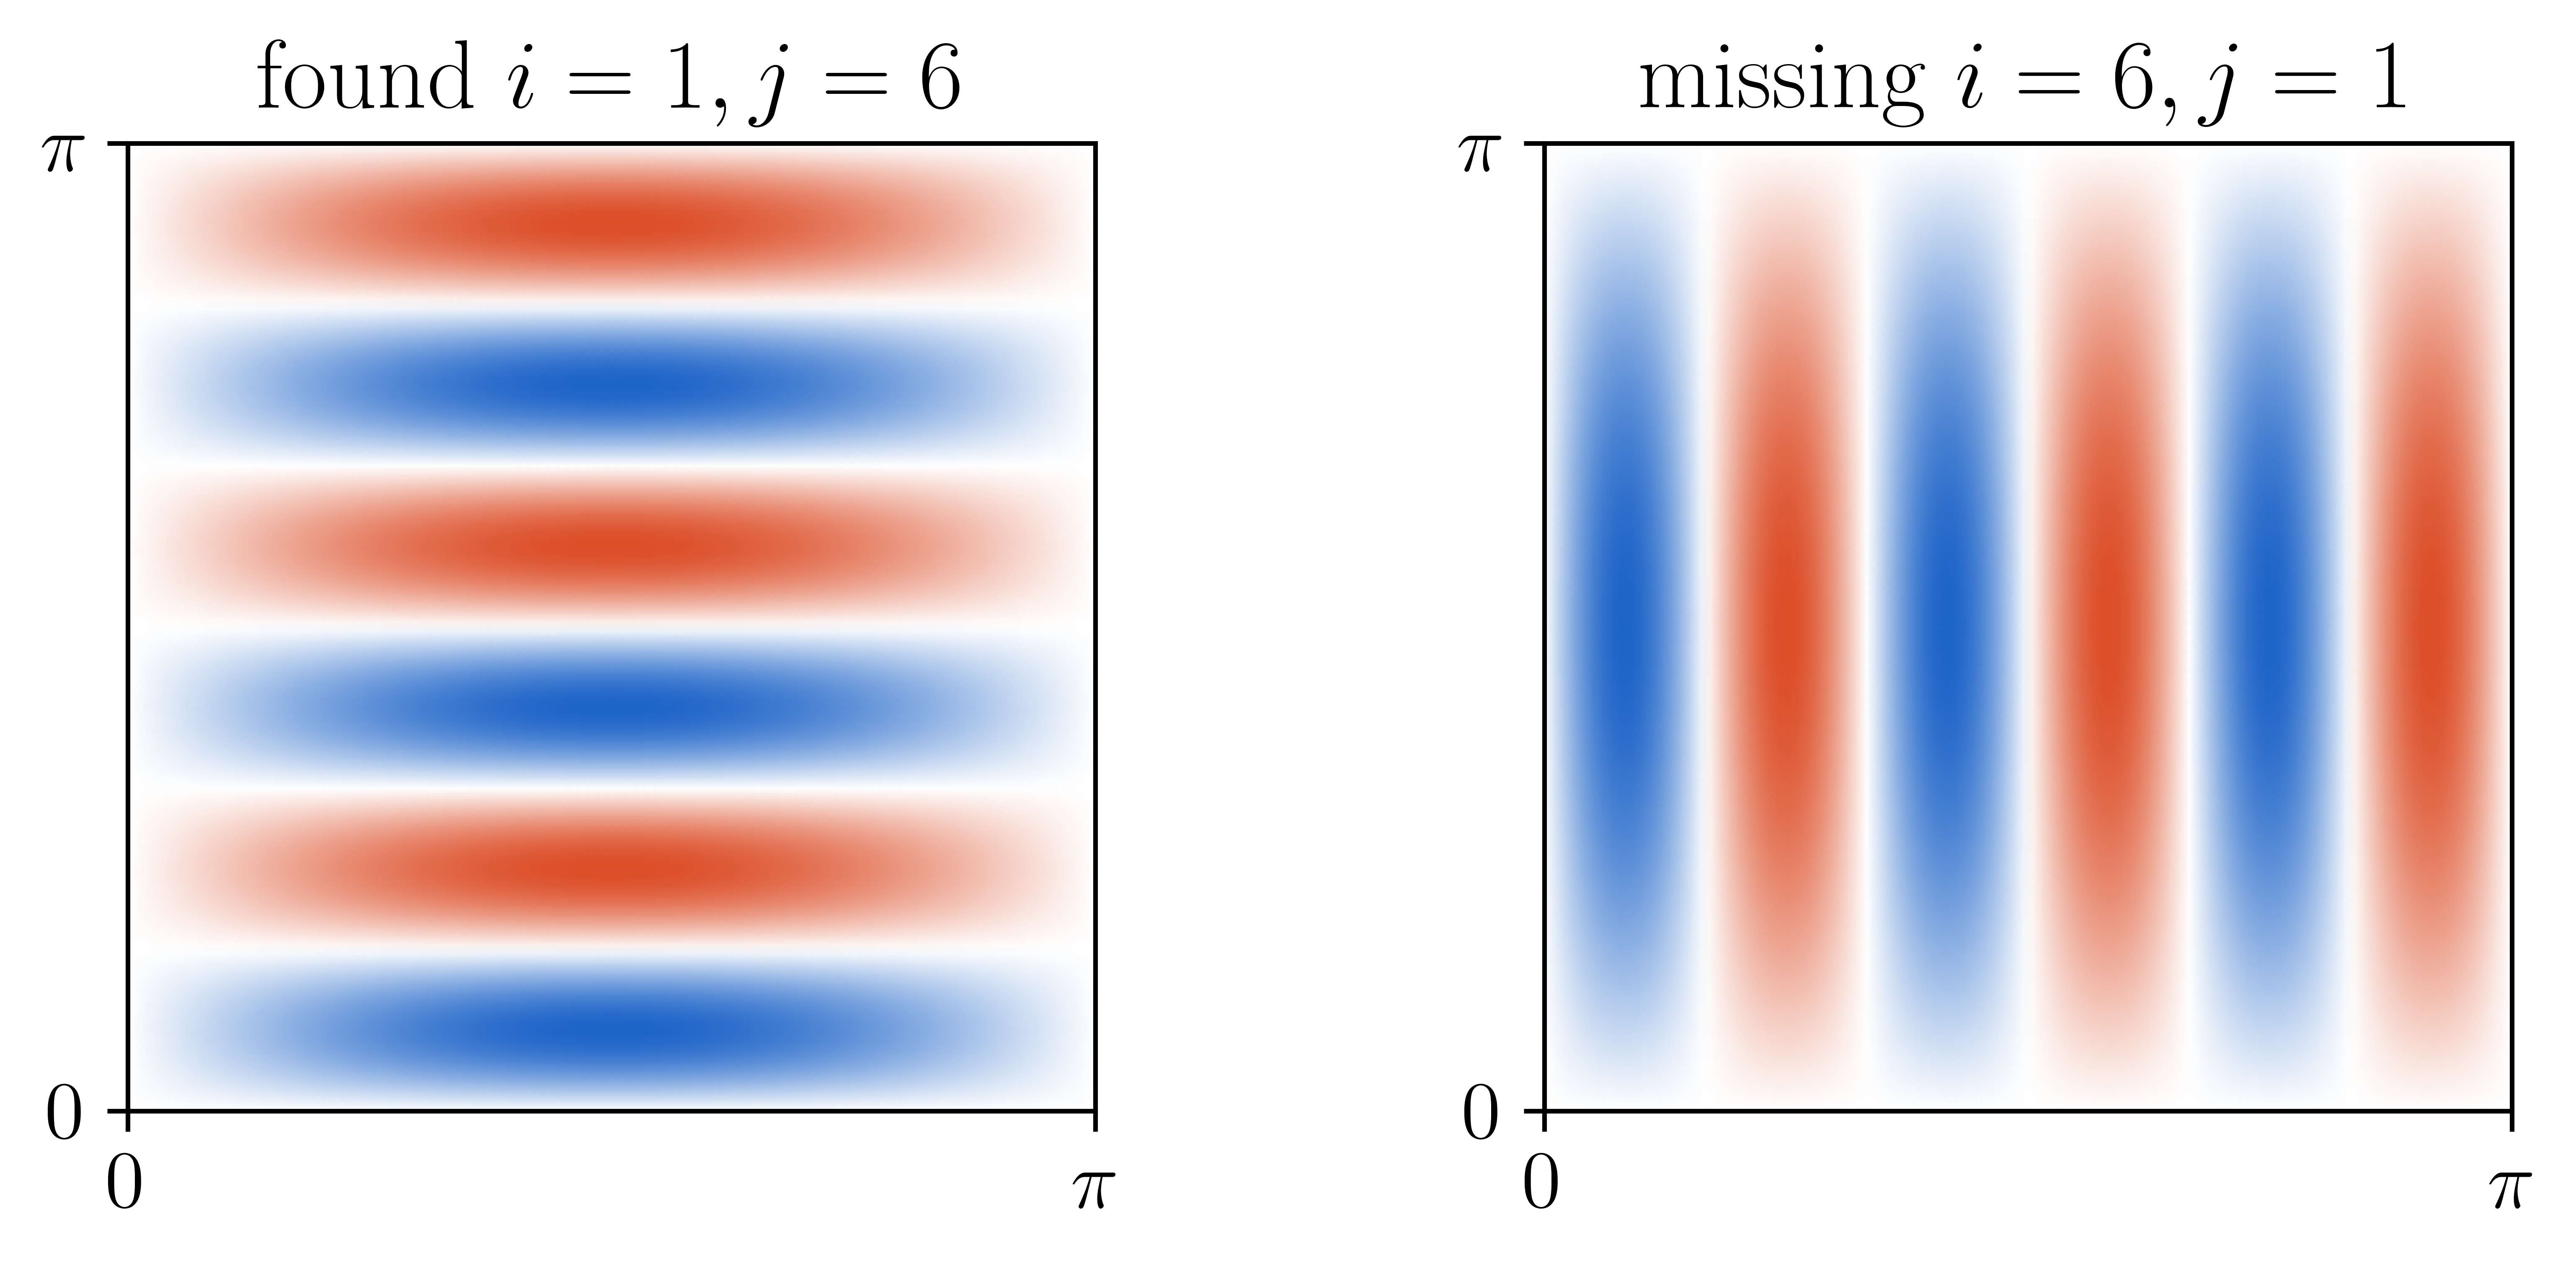
\includegraphics[width=\textwidth]{img/chapter3/experiments/zero_missing.png}
  \end{center}
  \caption{When using $N = 5$. On the left: the found $22^\text{nd}$ eigenfunction. On the right: the missing $23^\text{th}$ eigenfunction.}\label{fig:c3_experiment_zero_missing}
\end{figure}

The reason for these sudden wrong results can be found in the fact that the Schrödinger problem with zero potential on a rectangular domain is definitely an easy problem for this method. Upon close inspection, we have found that \pyslisetd{} only uses a total of three sectors on the whole domain, independent of the requested accuracy. On each sector, exactly the same one-dimensional problem is solved, yielding exactly the same basis functions $b_i(x) = \sin(i x)$. And coincidentally, the two-dimensional eigenfunction corresponding to $E = i^2 + j^2$ can be written as $\psi(x, y) = c(y) \sin(i x)$ for a $y$-dependent function $c(y)$. In summary for this method, by construction, the Schrödinger problem with zero potential gets solved exactly. Yet, for $N=5$ we see that $E_{22} = E_{23}$ is not found correctly. Notice that $E_{22} = E_{23} = 37 = 1^2 + 6^2$. When only five basis functions are considered on a sector, the necessary function $\sin(6 x)$ will not be present, and therefore this eigenvalue cannot be correctly found. As an illustration, figure~\ref{fig:c3_experiment_zero_missing} visualizes this missing eigenfunction.

Let us also address a possible concern: why did our method not detect this missing eigenvalue, using theorem~\ref{the:c3_counting_eigenvalues}? Our method checks how many times there was a linear combination of the propagated functions that vanishes. If an insufficient number of basis functions are used, no such vanishing combination will be found, and the index will not be correctly determined. Here, the importance of a sufficiently large basis is apparent.

To illustrate the use of \pyslisetd{} we present some sample code to solve this Schrödinger problem.
% \begin{noindent}
\begin{minted}{python}
from pyslise2d import Pyslise2D
from math import pi

problem = Pyslise2D(lambda x, y: 0, 0, pi, 0, pi,
                    tolerance=1e-8, N=10)
print(problem.eigenvaluesByIndex(0, 10))
\end{minted}
% \end{noindent}
This code will output a list of all eigenvalues as tuples. For each eigenvalue we get its index, the eigenvalue itself and its multiplicity. This multiplicity is numerically detected, thus this may be inaccurate. An eigenvalue can be present multiple times in the list to compensate.


\subsection{The harmonic oscillator potential}\label{sec:c3_experiment_harmonic}

As the zero potential is quite easy for this method, next we will consider the quantum harmonic oscillator with potential $V(x, y) = x^2 + y^2$. On the infinite domain $\RR^2$, the true eigenvalues are known to be
$$
  2, 4, 4, 6, 6, 6, 8, 8, 8, 8, 10, \dots, 10, 12, \dots
$$
The method does not support infinite domains, thus we will assume homogeneous Dirichlet boundary conditions on $\Omega = [-9.5, 9.5] \times [-9.5, 9.5]$. This allows a comparison to section~\ref{sec:c4_numerical_harmonic}.

Our implementation is relatively autonomous, there are only two parameters to study. First we can specify a tolerance to influence the automatic sector size selection. And second, we can influence the number of basis functions $N$ to use on each sector.

\begin{figure}
  \begin{center}
    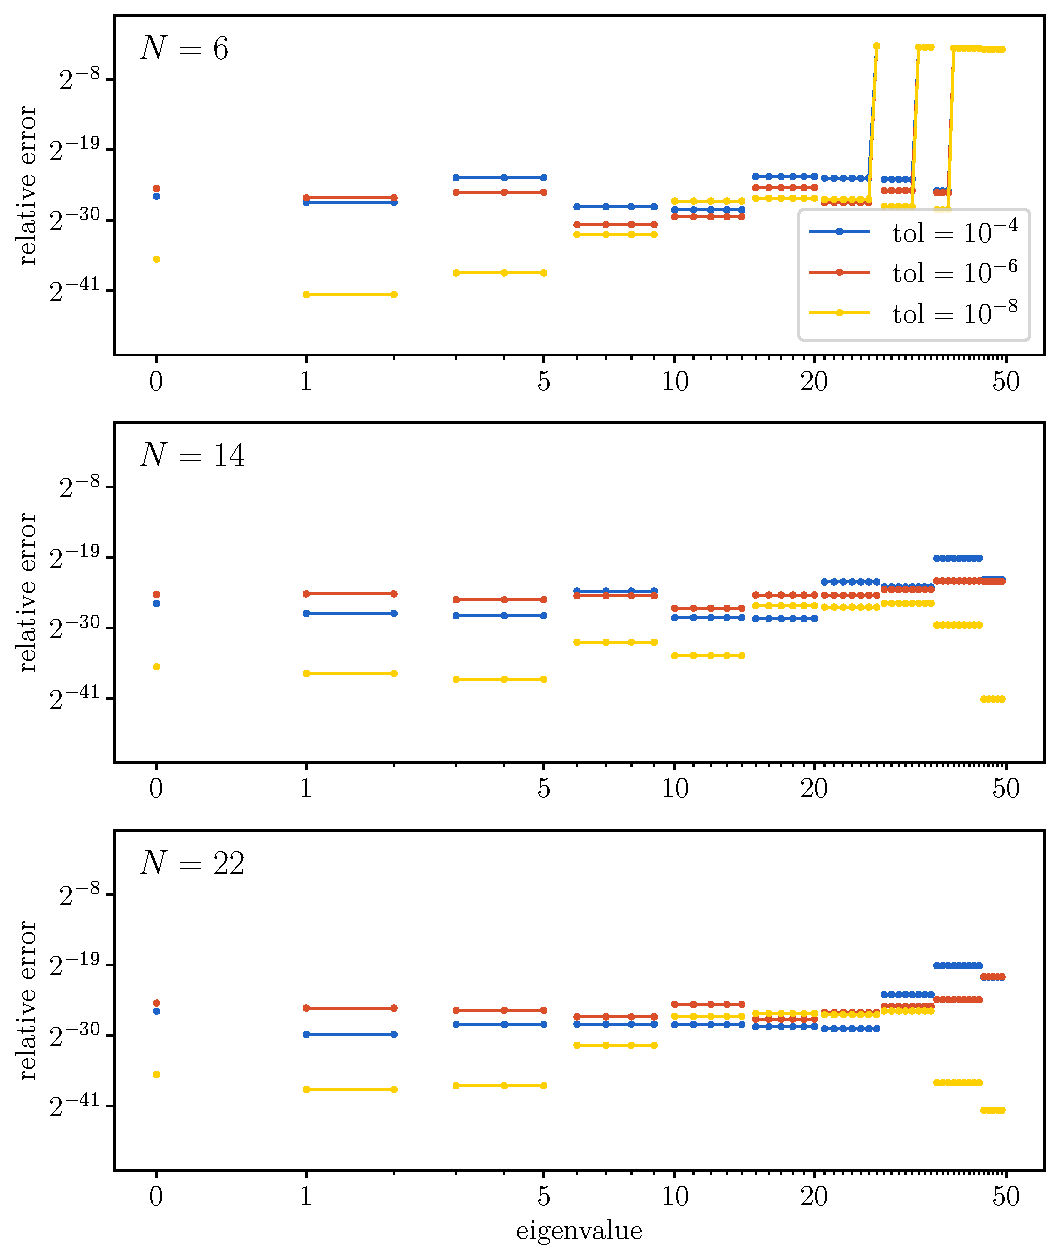
\includegraphics[width=\textwidth]{img/chapter3/experiments/harmonic.pdf}
  \end{center}
  \caption{A comparison of relative error of the first fifty eigenvalues of the harmonic oscillator problem for different basis sizes $N$ and requested tolerances $\text{tol}$. For $N=22$, the algorithm with different tolerances used respectively $19$, $29$ and $40$ sectors.}\label{fig:c3_experiment_harmonic}
\end{figure}

In figure~\ref{fig:c3_experiment_harmonic}, we provide a comparison of the relative error of the first few eigenvalues when varying these two parameters. The first thing we must remark is that our implementation has degenerate eigenvalue detection. This can be seen in the equal error for each of these eigenvalues.

For a small basis size ($N = 6$), we observe the same behavior as in figure~\ref{fig:c3_experiment_zero}. From a certain point onward, eigenvalues will be plain wrong. For the first fifty eigenvalues, this behavior disappears once $N$ is sufficiently large.

When we focus upon the first three eigenvalues, we see (as expected) that, if we lower the requested tolerance, the eigenvalue approximations become more accurate. However, for higher lying eigenvalues, this relation seems to disappear unexpectedly. This is concerning. It may suggest that there is still somewhere a source of inaccuracy which we are not controlling for. In section~\ref{sec:c3_conclusion_hypothesis}, we will present some hypotheses and deeper analysis for these results.

Ever the optimists, we also notice that for the first ten eigenvalues, our algorithm reaches an accuracy of $2^{-30} \approx 10^{-9}$. For the first twenty eigenvalues, we reach an accuracy of $2^{-21} \approx 10^{-7}$, for all $N$ visualized. These results are certainly impressive.

As a reference, the following code can be used to solve this problem.
% \begin{noindent}
\begin{minted}{python}
from pyslise2d import Pyslise2D

def V(x, y):
    return x * x + y * y

harmonic = Pyslise2D(V, -9.5, 9.5, -9.5, 9.5
                     tolerance=1e-8, N=14)
print(harmonic.eigenvaluesByIndex(0, 30))
\end{minted}
% \end{noindent}


\subsection{Ixaru's potential}\label{sec:c3_experiment_ixaru}

For the next example we follow~\cite{ixaru_new_2010} and study the problem from section~\ref{sec:c3_counting_ixaru}. Consider the Schrödinger problem with potential
$$
  V(x, y) = (1+x^2)(1+y^2)
$$
on the square domain $[-5.5, 5.5] \times [-5.5, 5.5]$ with homogeneous Dirichlet boundary conditions.

For this problem no analytical results are available. However, in~\cite{ixaru_new_2010} numerical results are reported.

By using \texttt{pyslise2d}, the code to solve this problem is quite straightforward.
% \begin{noindent}
\begin{minted}{python}
from pyslise2d import Pyslise2D

def V(x, y):
    return (1+x*x)*(1+y*y)

problem = Pyslise2D(V, -5.5,5.5, -5.5,5.5,
                    tolerance=1e-8)
problem.eigenvaluesByIndex(0, 12)
\end{minted}
% \end{noindent}

\begin{table}
  \centering
  \begin{tabular}{ln{2}{7}n{2}{10}}
    \toprule
                    & {Ixaru~\cite{ixaru_new_2010}} & {Our results} \\
    \midrule
    $E_{0}$         & 3.1959181                    & 3.195918111   \\
    $E_{1} = E_{2}$ & 5.5267439                    & 5.526744074   \\
    $E_{3}$         & 7.5578033                    & 7.557803572   \\
    $E_{4}$         & 8.0312723                    & 8.031272363   \\
    $E_{5}$         & 8.4445814                    & 8.444581756   \\
    $E_{6} = E_{7}$ & 9.9280611                    & 9.928061161   \\
    $E_{8} = E_{9}$ & 11.3118171                   & 11.311817614  \\
    $E_{10}$        & 12.1032536                   & 12.103253445  \\
    $E_{11}$        & 12.2011790                   & 12.201179825  \\
    $E_{12}$        & 13.3323313                   & 13.332332972  \\
    \bottomrule
  \end{tabular}
  \caption{\label{tab:ixaru_eigenvalues} The first few eigenvalues of the problem with potential $V(x,y) = (1+x^2)(1+y^2)$ on the domain $[-5.5; 5.5] \times [-5.5; 5.5]$.}
\end{table}

In table~\ref{tab:ixaru_eigenvalues}, our results are compared to the reference values calculated by Ixaru in~\cite{ixaru_new_2010}. There, the computation took $45$ seconds. Our values were computed within $1.4$ seconds on an Intel i7-8700K. Blindly comparing these run-times is ill-informed as the hardware is significantly different. Regardless, we are quite satisfied with the speed our program is able to achieve.

Upon close inspection of table~\ref{tab:ixaru_eigenvalues}, we remark that our results agree with these from~\cite{ixaru_new_2010} to all digits, except sometimes the last (two).

\begin{figure}
  \begin{center}
    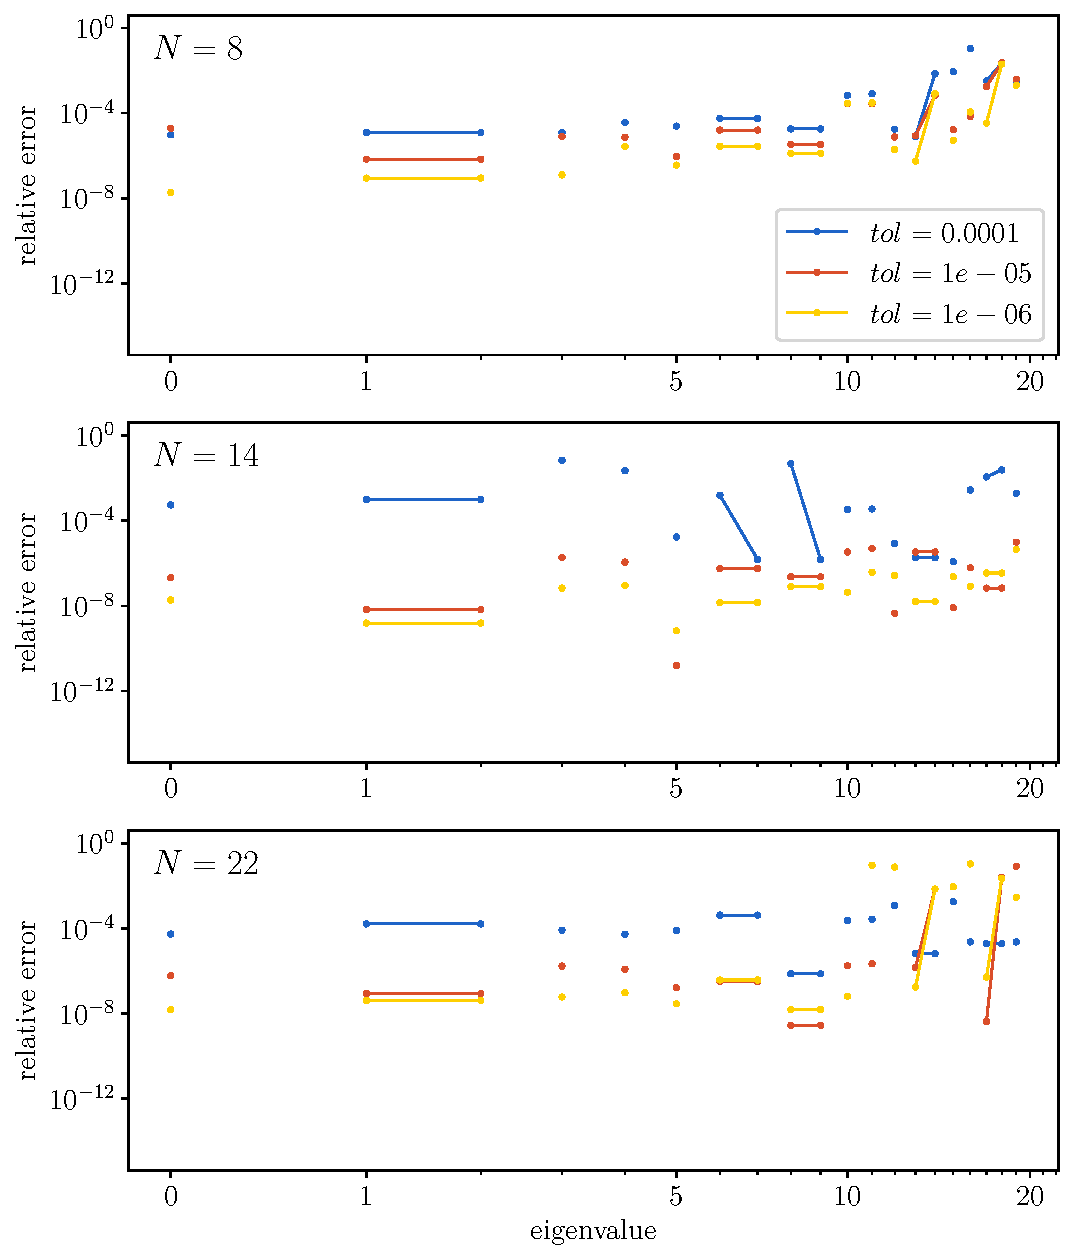
\includegraphics[width=\textwidth]{img/chapter3/experiments/ixaru.pdf}
  \end{center}
  \caption{A comparison of relative error of the first thirty eigenvalues of the Schrödinger problem with Ixaru's potential from section~\ref{sec:c3_experiment_ixaru} for different basis sizes $N$ and requested tolerances.}\label{fig:c3_experiment_ixaru}
\end{figure}

Alternative to a table of values, we plot the relative errors of the found eigenvalues for different basis sizes $N$ and requested tolerances in figure~\ref{fig:c3_experiment_ixaru}. As we observed numerical issues in the previous experiment, here the reference values were not computed with \pyslisetd{}, rather we employed our method from the next chapter. Some remarks can be made on figure~\ref{fig:c3_experiment_ixaru}. First, the same numerical issues as for the harmonic oscillator can be observed. The relative errors seem to plateau around $10^{-8}$, independent of which accuracy is requested, or the basis size used. Second, in all panels, we can observe a clear trend in the blue curve with $N = 6$: if the index of the eigenvalue becomes larger, the accuracy decreases. For the red curve with $N = 12$,  a similar trend can be suspected in the eigenvalues with index close to $30$.

Drawing conclusions with any certainty from these graphs is difficult. We believe these graphs to support the analysis of section~\ref{sec:c3_conclusion_hypothesis}.

\subsection{The H\texorpdfstring{é}{e}non--Heiles potential}\label{sec:c3_experiment_henon}

Another interesting example is the Hénon--Heiles potential. The corresponding Schrödinger problem is given by:
$$
  -\nabla^2 \psi + \left(x^2 + y^2 + \frac{\sqrt{5}}{30} y \left(3 x^2  - y^2\right)\right)\psi = E \psi \text{.}
$$

Following~\cite{braun_efficient_1996}, we impose homogeneous Dirichlet boundary conditions on the square $[-6, 6] \times [-6, 6]$. Our results are reported in table~\ref{tab:henon_heiles_eigenvalues}. The computation only took $1.3$ seconds, and the results are identical, within the available precision in~\cite{braun_efficient_1996}.

\begin{table}
  \centering
  \begin{tabular}{ln{1}{6}n{1}{10}}
    \toprule
                      & {Braun et al.~\cite{braun_efficient_1996}} & {Our results} \\
    \midrule
    $E_{0}$           & 0.998595                                   & 0.9985947661  \\
    $E_{1} = E_{2}$   & 1.990077                                   & 1.9900767814  \\
    $E_{3}$           & 2.956243                                   & 2.9562429806  \\
    $E_{4} = E_{5}$   & 2.985326                                   & 2.9853263715  \\
    $E_{6} = E_{7}$   & 3.925964                                   & 3.9259638565  \\
    $E_{8}$           & 3.982417                                   & 3.9824172948  \\
    $E_{9}$           & 3.985761                                   & 3.9857610624  \\
    $E_{10}$          & 4.870144                                   & 4.8701435890  \\
    $E_{11} = E_{12}$ & 4.898644                                   & 4.8986454644  \\
    $E_{13} = E_{14}$ & 4.986251                                   & 4.9862512850  \\
    $E_{15}$          & 5.817019                                   & 5.8170190699  \\
    $E_{16}$          & 5.817027                                   & 5.8170279899  \\
    \bottomrule
  \end{tabular}
  \caption{\label{tab:henon_heiles_eigenvalues}  The first few eigenvalues of the problem with potential $V(x,y) = x^2 + y^2 + \frac{1}{6\sqrt{5}} y \left(3 x^2  - y^2\right)$ on the domain $[-6; 6] \times [-6; 6]$. The results are reported divided by $2$ to provide compatibility with~\cite{braun_efficient_1996}.}
\end{table}

By now the code for solving this problem will look familiar.

% \begin{noindent}
\begin{minted}{python}
from pyslise2d import Pyslise2D
from math import sqrt

def V(x, y):
    return x*x + y*y + sqrt(5)/30 * y * (3*x*x - y*y)

problem = Pyslise2D(V, -6,6, -6,6, tolerance=1e-8)
problem.eigenvaluesByIndex(0, 16)
\end{minted}
% \end{noindent}

With our program, also the eigenfunctions can be computed. This is demonstrated in figure~\ref{fig:henon_heiles_eigenfunction}.
\begin{figure}
  \begin{center}
    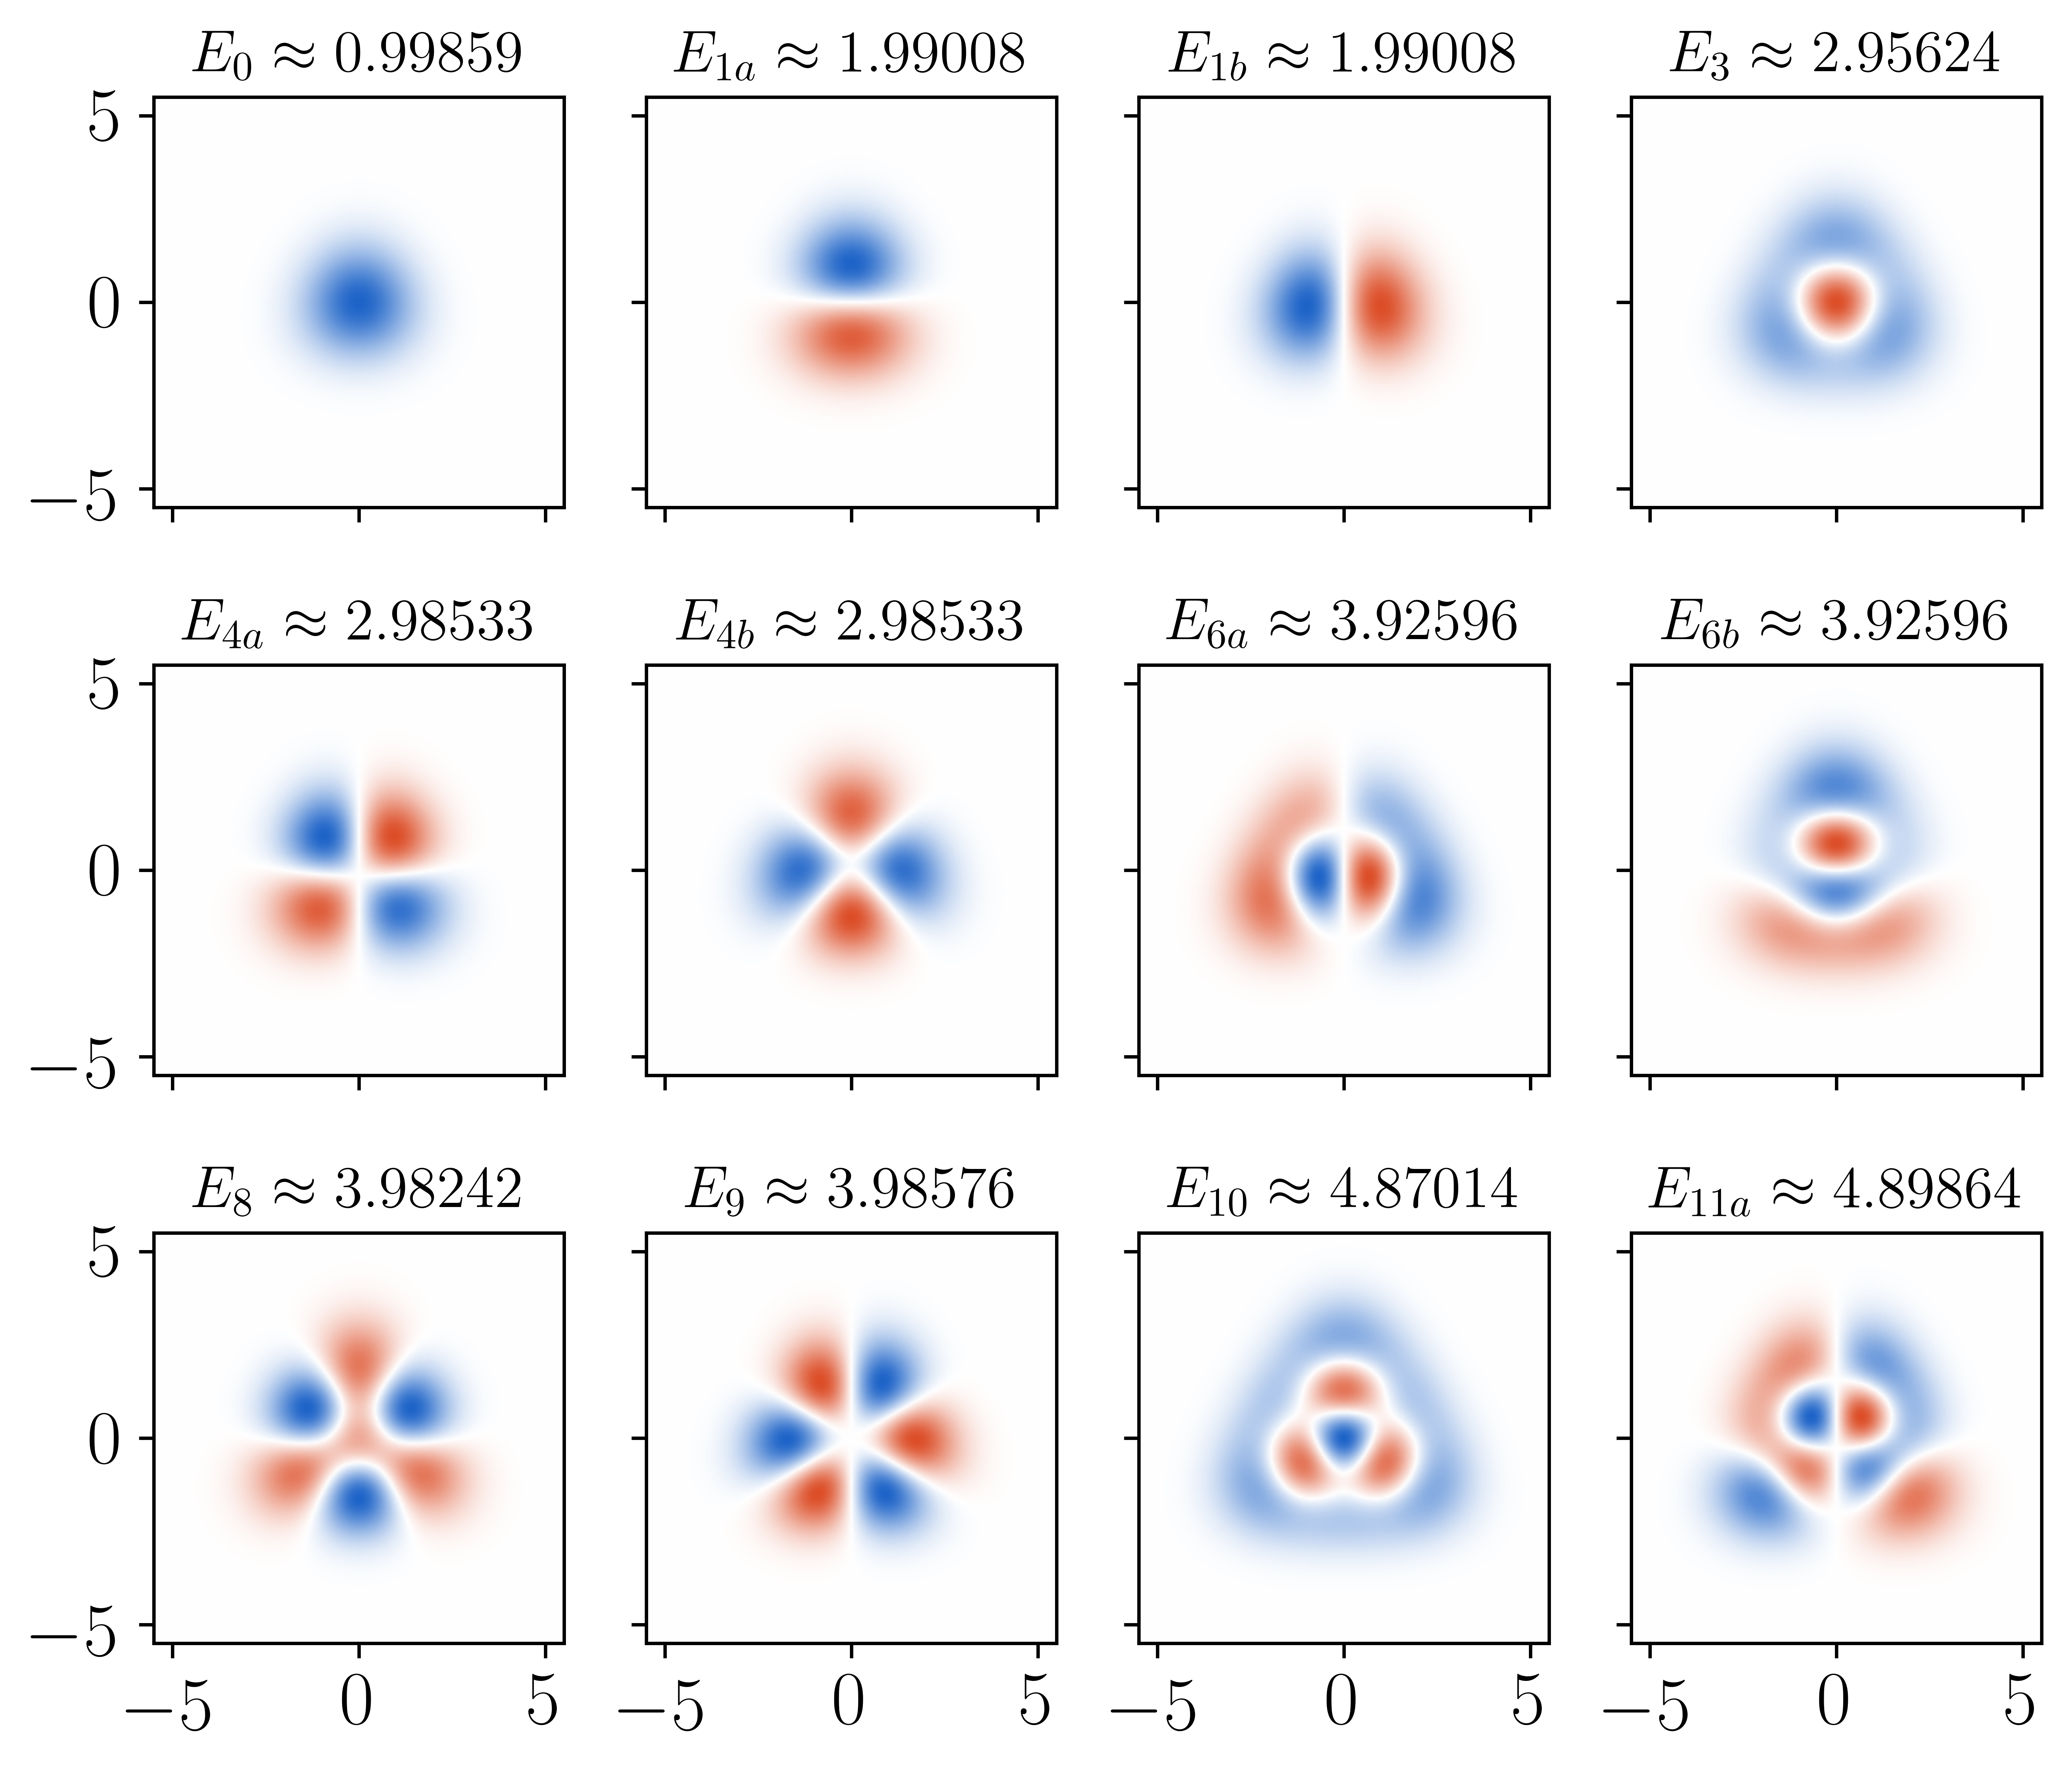
\includegraphics[width=\linewidth]{img/chapter3/experiments/henon_heiles_eigenfunctions.png}
    \caption{\label{fig:henon_heiles_eigenfunction} The first twelve eigenfunctions of the Schrödinger problem with the Hénon--Heiles potential on $[-6, 6]\times[-6,6]$.}
  \end{center}
\end{figure}

Here we have opted to not include similar figures to visualize the relative errors as in the previous experiments. These graphs do not let us gain any more new insights.

\subsection{Analyzing unexpected numerical behavior}\label{sec:c3_conclusion_hypothesis}

In figure~\ref{fig:c3_experiment_harmonic}, we have seen some strange behavior of the relative error of the eigenvalues in function of the tolerance and basis size. In some cases, the relative error of the eigenvalues found, did not decrease if a larger basis on each sector or more sectors were used. It was clear that something unexpected was happening. Ideally for numerical methods, we should observe an increase in accuracy when more accurate intermediate results are used.

Discovering where we lost accuracy, is a real challenge. As chapter~\ref{cha:c2} contains many numerical experiments up to extreme precision, it would be very surprising if the basis functions would be the cause of these inaccuracies. Another possible source could be the propagation of $\vb{c}^{(k)}$ from~\eqref{equ:c3_coupled_system} within a sector. Yet, our implementation of \matscs{} has been thoroughly tested. Furthermore, numerical issues with the propagation would more likely lead to a large error, which in turn would manifest itself as an abundance of sectors, which is not the case. In section~\ref{sec:c3_experiments_zero}, we have studied the Schrödinger problem with zero potential. Here, our program was able to reach machine precision without much trouble. This likely confirms that basis functions are correctly calculated and that propagation with the coupled system of Schrödinger equations seems to work.

Of course, no sufficiently interesting program is bug-free. The programs we have developed in this thesis are definitely not an exception. However, bugs in numerical software lead most of the time to completely wrong results or slow convergence. The behavior seen in figure~\ref{fig:c3_experiment_harmonic} is atypical, to say the least.

\begin{figure}
  \begin{center}
    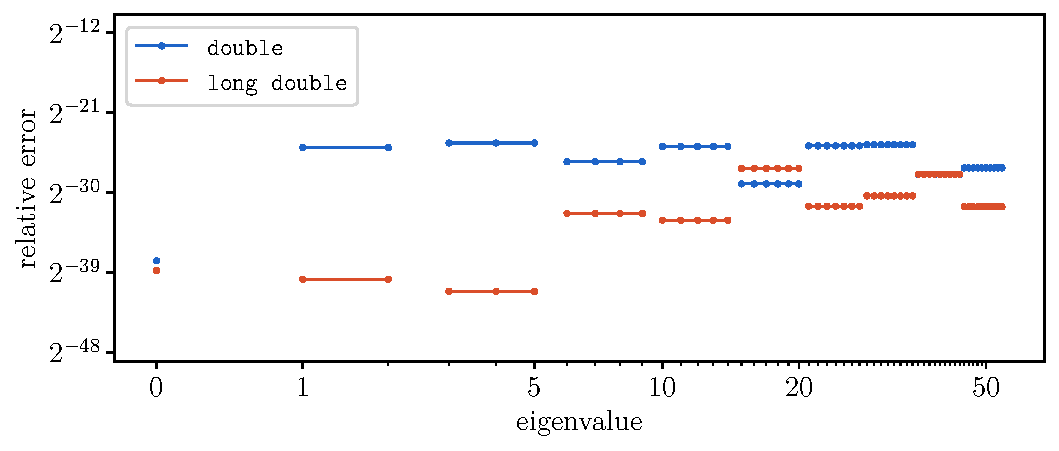
\includegraphics[width=\textwidth]{img/chapter3/experiments/harmonic_analysis.pdf}
    \caption{We have solved the harmonic oscillator problem from section~\ref{sec:c3_experiment_harmonic} once again with $N = 22$ and a requested tolerance of $10^{-11}$. The blue points represent the results calculated with \texttt{double}-precision. The red points are calculated in \texttt{long double}-precision.}\label{fig:c3_harmonic_analysis}
  \end{center}
\end{figure}

Yet, more analysis is warranted. To locate the source of the numerical difficulties, we present figure~\ref{fig:c3_harmonic_analysis}. Here, we have run our program  for the harmonic oscillator problem from before with a tolerance of $10^{-11}$. Once the computation was executed with the standard \texttt{double}-precision\footnote{Numbers with a $53$ bit mantissa.}, we have repeated the same calculation with the same parameters, but using \texttt{long double}-numbers\footnote{This is the x86 extended precision format with a mantissa of $65$ bit.}. As a tolerance of $10^{-11}$ is well within the range of \texttt{double}-precision numbers, we expect to see (almost) identical results. However, this is not the case. The results obtained with the datatype with higher precision are for most eigenvalues much more accurate.

Interpreting these results is not straightforward. It is hard to determine exactly the source of the differences from figure~\ref{fig:c3_harmonic_analysis}. Due to the use of \cpp{}'s template parameters (see section~\ref{sec:c2_generalizing_scalar}), exactly the same code is being executed for all numeric types. It would be also extremely unlikely if this would be a logical or mathematical error, as a higher precision numeric type does reach more accurate results, with all other parameters being equal.

So, what can it be? Our best guess is that this is an inherent numerical instability when using the method studied in this chapter. We see many possible sources of this numeric instability, so finding the true culprit may be insurmountably difficult. One possibility could be that in the huge formulae we implemented for propagation of coupled systems of Schrödinger equations, some cancellation occurs. To demonstrate this possibility we take a closer look at a single term in these giant formulae:
$$
  \dots + \left(-\frac{1}{24}\vb{V_0}\vb{V_1} + \frac{1}{24} \vb{V_1}\vb{V_0}\right) h^4 + \dots \text{.}
$$
Here $\vb{V_0}$ and $\vb{V_1}$ are matrices used in the polynomial approximation of the matrix potential $\vb{V}(x)$. If $\vb{V_0}$ and $\vb{V_1}$ almost commute, $\vb{V_0}\vb{V_1}$ and $\vb{V_1}\vb{V_0}$ will be close together, and cancellation becomes an issue. This is only one example of many such terms, commutators are extremely common in these huge expressions.

In section~\ref{sec:c3_calculate_vk}, we have developed a technique to symbolically calculate the integrals present in the definition of $\vb{V}^{(k)}(y)$. Here we were careful in ensuring numerical stable recursive formulae. Another possibility for the numeric difficulties could be that we still were not careful enough. It could be that in these calculations a numeric instability becomes impactful if more accuracy is requested.

Or, another possible culprit can maybe be found in the propagation of $\vb{c}^{(k)}(y)$. If many basis functions are used on a sector, there arises a large discrepancy in the behavior of the propagation of different elements of $\vb{c}^{(k)}(y)$. The first elements (corresponding to small eigenvalues) will exhibit an oscillatory behavior, but the last elements (corresponding to much larger eigenvalues) exhibit an exponential behavior. This discrepancy is already partly mitigated by regularly rescaling the propagated matrix, however this rescaling is only (and can only be) done on the boundary of sectors.

In summary, we were unable to exactly pinpoint the source of the particular unexpected results of figure~\ref{fig:c3_experiment_harmonic}. However, some possibilities were discussed. More importantly, all these possibilities have in common that they are extremely difficult or nearly impossible to fix.


\section{Conclusions}

In this chapter, we have studied the method introduced by Ixaru in~\cite{ixaru_new_2010} for two-dimensional time-independent Schrödinger equations. The original work presented an intriguing innovative method accompanied by a promising numerical example. Section~\ref{sec:c3_ixarus_method} presents an overview of this method as first described. In section~\ref{sec:c3_improvements}, we proudly presented our additions and improvements to this method. In particular, we have devised a way to reliably determine the index of an eigenvalue. For this, we developed some new theory in section~\ref{sec:c3_index_of_e}.

Section~\ref{sec:c3_experiments} was dedicated to some numerical experiments. In this thesis, in contrast to an article, we have the luxury to take the time for a much deeper dive into some numerical experiments. As such, in this last section, we have unearthed some numerical difficulties present in this method. Attaining extremely high accuracies proved to be difficult. In section~\ref{sec:c3_conclusion_hypothesis}, these numerical issues were analyzed.

Now, it is easy to conclude with ``more research is needed''. However, in this thesis we are not interested in such a meaningless cop-out. We are sufficiently brave to add some nuance and (maybe unpopular) opinion. On the one hand, this method is definitely not without merit. It contains many invaluable ideas, making it a unique view onto the subject. On the other hand however, I am internally conflicted about whether this method is worth pursuing. In the next chapter we will start with the analysis of a relatively simple technique based upon a finite difference scheme. We will see that this technique is much easier to implement, is able to reach much higher accuracies, and all this without significantly more computation time.

Concluding this chapter by declaring the last few years of research that we invested in the described method a waste of time, is too harsh. We were able to undoubtedly improve this method and discovered some new, more widely applicable theoretical results in the process.

In scientific research we definitely need new and innovative ideas such as Ixaru's method, as described in this chapter. These groundbreaking ideas are a breeding ground of and a jumping point to more new ideas. During the development of this thesis, I have found one of the more challenging aspects of scientific research to be the evaluation of ideas. With this I mean, recognizing valuable ideas and spending time developing them, but also the opposite: sufficiently early deciding that an idea is maybe not as promising as once hoped.

Let me finally conclude this chapter by writing something one rarely reads in scientific articles: I do not know whether more research is really required.

\stopchapter


% !TeX root = chapter4_2d_new.tex
% !TeX root = thesis.tex
\ifdefined\UtilIncluded
  \renewcommand{\startchapter}[1]{}
  \renewcommand{\stopchapter}{}
  \renewcommand{\undefinedlabel}[2]{}
\else

\newcommand{\startchapter}[1]{\begin{document}\setcounter{chapter}{#1}\addtocounter{chapter}{-1}}
\newcommand{\stopchapter}{\printbibliography[title=Bibliography,heading=bibintoc]\end{document}}


\documentclass{book}
\usepackage[utf8]{inputenc}


\usepackage{geometry}
\geometry{
  papersize={170mm,240mm},
}

\usepackage{amsfonts,amsmath, amsthm, amssymb, mathtools}
\usepackage{xspace}
\usepackage[hidelinks,bookmarks,pdfusetitle]{hyperref}
\usepackage{listings}
\usepackage[pdftex]{graphicx}
\usepackage{bm}
\usepackage[english]{babel}
\usepackage{caption}
\usepackage{subcaption}
\usepackage[usenames,dvipsnames]{xcolor}
\usepackage{physics}
\usepackage{multicol}
\usepackage{xstring}
\usepackage{pythonhighlight}
\usepackage{parskip}
\usepackage{thmtools}
\usepackage{relsize}
\usepackage{bookmark}
\usepackage{lmodern}
\usepackage{ifthen}
\usepackage{biblatex}
\usepackage{microtype}
\usepackage{csquotes}
\usepackage{numprint}
\usepackage{mleftright}
\npthousandsep{{\ifmmode\mskip2mu\else\hskip0.2em\fi}}
\npdecimalsign{.}

\addbibresource{references.bib}

\newtheorem{theorem}{Theorem}[chapter]
\newtheorem{lemma}[theorem]{Lemma}
\newtheorem{corollary}[theorem]{Corollary}
\newtheorem{definition}[theorem]{Definition}

\DeclareRobustCommand{\oneD}{{1{\relsize{-1}D}}\xspace}
\DeclareRobustCommand{\twoD}{{2{\relsize{-1}D}}\xspace}
\DeclareRobustCommand{\threeD}{{3{\relsize{-1}D}}\xspace}
\DeclareRobustCommand{\cpp}{{{C\nolinebreak[4]\hspace{-.05em}\raisebox{.4ex}{\relsize{-3}\textbf{++}}}\xspace}}
\pdfstringdefDisableCommands{%
  \def\cpp{C++}%
  \def\oneD{1D}%
  \def\twoD{2D}%
  \def\threeD{3D}%
}

\newcommand{\longchapter}[2][]{%
  \chapter[#2]{#2}%
  \ifthenelse{\equal{#1}{}}{}{\chaptermark{#1}}}

\newcommand{\NN}{\mathbb{N}}
\newcommand{\ZZ}{\mathbb{Z}}
\newcommand{\QQ}{\mathbb{Q}}
\newcommand{\QQbar}{\overline{\mathbb{Q}}}
\newcommand{\RR}{\mathbb{R}}
\newcommand{\CC}{\mathbb{C}}

\newcommand{\Eigen}{\texttt{Eigen}}

\newcommand{\sage}{\texttt{sage}\xspace}

\newcommand{\hamiltonian}{\mathcal{H}}

\newcommand{\transposesign}{\intercal}
\newcommand{\transpose}[1]{{#1}^\transposesign}
\newcommand{\adjointsign}{\text{H}}
\newcommand{\adjoint}[1]{{#1}^\adjointsign}

\newcommand{\xmin}{{x_{\text{min}}}}
\newcommand{\xmax}{{x_{\text{max}}}}
\newcommand{\ymin}{{y_{\text{min}}}}
\newcommand{\ymax}{{y_{\text{max}}}}

\newcommand{\Cbottom}{\vb{C}_\text{bottom}}
\newcommand{\Ctop}{\vb{C}_\text{top}}
\newcommand{\ubottom}{\vb{u}_\text{bottom}}
\newcommand{\utop}{\vb{u}_\text{top}}

\DeclareMathOperator{\diag}{diag}
\DeclareMathOperator{\tridiag}{tridiag}
\DeclareMathOperator{\eigs}{eigs}
\DeclareMathOperator*{\argmin}{arg\,min}
\DeclareMathOperator{\Ai}{Ai}
\DeclareMathOperator{\Bi}{Bi}
\DeclareMathOperator{\OO}{\mathcal{O}}

% https://tex.stackexchange.com/a/18192/163747
\makeatletter
\newcommand{\undefinedlabel}[2]{%
  \protected@write \@auxout {}{\string \newlabel {#1}{{#2}{\thepage}{#2}{#1}{}} }%
  \hypertarget{#1}{}
}
\makeatother

\fi
\gdef\UtilIncluded{}


\startchapter{4}
\undefinedlabel{cha:c2}{2}
\undefinedlabel{cha:c3}{3}
\undefinedlabel{sec:c3_eigenvalues_wrt_domain_analysis}{3.-.-.-}
\undefinedlabel{sec:c3_experiment_henon}{3.-.-}
\undefinedlabel{sec:c3_calculate_vk}{3.-.-}

\longchapter[New methods]{New methods for the \twoD time-independent Schrödinger equation}\label{cha:c4}

In chapter \ref{cha:c2} we have studied the constant perturbation methods. We have seen a brief history about these CP-methods, as well as a thorough overview about how these methods can be implemented. The numerical examples illustrated the benefits and demonstrated the accuracy of the studied techniques.

Chapter \ref{cha:c3} was dedicated to the treatment of a recent method to solve the time-independent two-dimensional Schrödinger equation. This method aims to use the strengths of the constant perturbation methods for higher dimensional problems. This new method is promising, and we developed many improvements upon the original idea.

One of the unique powers of the CP-methods is their ability to not only compute low eigenvalues accurately, but even increase accuracy for higher eigenvalues. For Sturm-Liouville problems there are methods which can accurately compute low eigenvalues ({\color{red}to do: reference to simple methods}) and there are methods which are accurate for higher eigenvalues (e.g. asymptotic methods \cite{kuzmina_asymptotic_2000,zhukova_asymptotic_2020}). A CP-method, however, is one of few, if not the only, technique which is accurate for low as well as high eigenvalues.

For two dimensions, this property did not translate cleanly. The method described in chapter \ref{cha:c3} tries to capture this by considering solutions of a one-dimensional Schrödinger problem in the $x$-direction, while a method for a coupled system of Schrödinger equations has been used in the $y$-direction. In theory this method is capable of computing any eigenvalue. In practice, this is not the case. A two-dimensional eigenfunction is represented as a linear combination $\sum_{i} c_i(y) \beta_i(x)$ of one-dimensional basis functions $\beta_i(x)$. This basis is well-chosen, such that even a few functions can already describe a two-dimensional eigenfunction sufficiently well. When implementing this, the basis has to be finite. As eigenfunctions corresponding to higher eigenvalues will become more and more oscillatory, the chosen finite basis will no longer be able to express all necessary details.

That the basis is finite, thus limits the accuracy for higher eigenvalues, which negates one of the strongest benefits of the employed CP-methods. As such, we believe that the perfect method for the more-dimensional time-independent Schrödinger equation is one which does not decrease in accuracy as the higher eigenvalues are requested. Just like the CP-methods are for the one-dimensional case. Developing such a method will, most likely, require new and very complicated formulae.

For clarity, we did not develop such a perfect method. But in the last few years I've played with the idea... In section \ref{c4:sec_utopy} we will present some ideas for such a method. Some of which, someone, somewhere, may find inspirational.

More realistically, during our research into the method of Ixaru, we have found other work, also focussing upon the time-independent Schrödinger problem. These ideas and methods have inspired us to develop our own technique. The new methods we propose try to fix or mitigate some issues present in the other methods.

    {\color{red} To do: list other methods}

\section{Inspiration}

After careful implementation and thorough testing of Ixaru's method from chapter \ref{cha:c3}, I could browse through the literature with renewed appreciation for the Schrödinger problem. When researching that method, many obstacles and challenges arose. It was an interesting task to balance computation time, symbolic formulas and numerical accuracy. So with this in mind, I came across \cite{wang_new_2009} by Wang and Shao.

In this article the authors proposed a new kind of discretization scheme for solving two-dimensional time-independent Schrödinger equations. Before studying the details of the method, I like to review their numerical results. They tested the algorithm on two potential functions. First, the harmonic oscillator was considered. Schrödinger problems with this potential function are not extremely difficult, but they capture some of the challenges that numerical algorithms may face, while still having symbolic solutions for the eigenvalues. Second, they provided results for the Hénon-Heiles potential. Here, the exact solutions are not known, but reliable approximations exist. For both potentials their results were quite impressive. They reached a high accuracy for a significant number of eigenvalues without using excessive computation time.

But the thing that strikes me most about \cite{wang_new_2009} is the simplicity of the method. They constructed formulas for a discrete approximation on a grid. Finding these kinds of results within the literature is disheartening and inspirational at the same time. At first glance they were able to reach higher accuracy with a simpler method than Ixaru's work \cite{ixaru_new_2010} and our improvements \cite{baeyens_improvements_2022} to it. Before throwing away all our work, and declaring \cite{wang_new_2009} to be superior, let us analyze it ourselves.

\subsection{A finite difference scheme}

As in chapter \ref{cha:c3}, we are considering the Schrödinger equation
\begin{equation}\label{equ:c4_schrodinger}
    -\psi''(x, y) + V(x, y) \psi(x, y) = \lambda \psi(x, y)
\end{equation}
on a rectangular domain $\Omega = [\xmin, \xmax] \times [\ymin, \ymax]$ with homogeneous Dirichlet boundary conditions, so $\psi(x, y) = 0, \forall (x, y) \in \dOmega$. The potential $V(x, y)$ is known and eigenvalues $\lambda$ with corresponding eigenfunctions $\psi(x, y)$ which satisfy \eqref{equ:c4_schrodinger} are sought.

In \cite{wang_new_2009} the authors discretize the domain $\Omega$ with an equidistant $n_x \times n_y$ grid. With this, they approximate the second partial derivative of a function $\psi(x, y)$ with, what they call, a new scheme:
$$
    {\pdv[2]{}{x}}\psi(x, y) = -\frac{1}{h^2}\sum_{i=-N_x}^{N_x} c_i \psi(x + ih, y)\text{.}
$$
In this expression $h$ is the $x$-step of the equidistant grid. An analogous formula for the second partial derivative of $\psi(x, y)$ with respect to $y$ is proposed, with $y$-step $\eta$:
$$
    {\pdv[2]{}{y}}\psi(x, y) = -\frac{1}{\eta^2}\sum_{i=-N_y}^{N_y} c_i \psi(x, y + i\eta)\text{.}
$$

To determine the value of $c_i$, the authors propose to assume $N = N_x = N_y$ and use the Taylor series expansion of the left-hand side of
$$
    \left({\pdv[2]{}{x}} + {\pdv[2]{}{y}}\right)\psi(x, y) = -\frac{1}{h^2} \sum_{i=-N}^{N} c_i \left(\psi(x+ih, y) + \left(\frac{h}{\eta}\right)^2\psi(x, y+i\eta)\right)\text{.}
$$
In \cite{wang_new_2009} the coefficients $c_i$ for $N_q = 3, 4, 5, 6$ are provided. For points close to the boundary of the domain, the authors propose to assume the unknown eigenfunction $\psi(x, y)$ will always be identically zero outside the domain $\Omega$. With this assumption, the same formulae can be used for every point in the discretization, even those close to the boundary.

Using these formulae the problem now approximates to a simple, albeit very large, square matrix eigenvalue problem.
\begin{equation}\label{equ:c4_fd_sparse_matrix}
    \left(-\vb{D}_{n_x} \otimes \vb{I}_{n_y} - \vb{I}_{n_x} \otimes \vb{D}_{n_y} +  \diag\begin{pmatrix}V(x_1, y_1) \\ V(x_1, y_2) \\ \vdots \end{pmatrix} \right)\vb{u} = \lambda \vb{u}
\end{equation}
Here, $\vb{D}_{n_x}$ is the symmetric Toeplitz\footnote{A matrix is called Toeplitz if each diagonal only contains a constant value. In other words, a matrix $\vb{A}$ is Toeplitz if it can be written as follows. $\vb{A}$ is a symmetric Toeplitz matrix if $a_{-i} = a_i$. $$\begin{pmatrix} a_0 & a_1 & a_2 & \dots \\ a_{-1} & a_0 & a_1 & \ddots \\ \vdots & \ddots & \ddots & \ddots \end{pmatrix}$$} $n_x \times n_x$ matrix with the first row $\begin{pmatrix} c_0 & c_1 & \dots & c_{N_x} & 0 & \dots \end{pmatrix}$. Analogous for $\vb{D}_{n_y}$. The $n\times n$ identity matrix is denoted as $\vb{I}_n$. The operation $\cdot \otimes \cdot$ is the Kronecker product\footnote{The Kronecker product of the $m\times m$ matrix $\vb{A}$ and the $n\times n$ matrix $\vb{B}$ is the following $(m+n)\times (m+n)$ block matrix: $$ \vb{A} \otimes \vb{B} = \begin{pmatrix} A_{1,1} \vb{B} & A_{1,2} \vb{B} & \dots \\ A_{2,1} \vb{B} & A_{2,2} \vb{B} & \\ \vdots & & \ddots \end{pmatrix} $$}. And finally, the vector of unknowns $\vb{u}$ is the approximation of $\psi$ in each of the grid points: $\vb{u} \approx \transpose{\begin{pmatrix} \psi(x_1, y_1) & \psi(x_1, y_2) & \dots \end{pmatrix}}$. The matrix on the left-hand side of \eqref{equ:c4_fd_sparse_matrix} can be directly computed. It is valuable to note that most of the entries of this matrix will be zero, so considering it as a sparse matrix is preferred. Many classical, well tested solvers exist for sparse eigenvalue problems. The authors of \cite{wang_new_2009} have used algorithms provided by \mathematica\cite{Mathematica}.

Before reviewing, and recalculating their numerical results, I want to take the time to thoroughly analyze their formulae. Using an equidistant grid and coefficients which optimize for the Taylor series of the function in question, is oddly reminiscent of finite difference approximations. To confirm this similarity we have calculated the central finite difference approximations of the second order derivative.

The following table contains the first few central symmetric finite differences.
\begin{center}
    \begin{tabular}{r|ccccccccccc}
Order & $c_0$ & $c_{-1}=c_{1}$ & $c_{-2}=c_{2}$ & $c_{-3}=c_{3}$ & $c_{-4}=c_{4}$ & $c_{-5}=c_{5}$\\[2pt]\hline
2 & $-2$ & $1$ & & & &\\[4pt]
4 & $- \frac{5}{2}$ & $\frac{4}{3}$ & $- \frac{1}{12}$ & & &\\[4pt]
6 & $- \frac{49}{18}$ & $\frac{3}{2}$ & $- \frac{3}{20}$ & $\frac{1}{90}$ & &\\[4pt]
8 & $- \frac{205}{72}$ & $\frac{8}{5}$ & $- \frac{1}{5}$ & $\frac{8}{315}$ & $- \frac{1}{560}$ &\\[4pt]
10 & $- \frac{5269}{1800}$ & $\frac{5}{3}$ & $- \frac{5}{21}$ & $\frac{5}{126}$ & $- \frac{5}{1008}$ & $\frac{1}{3150}$
\end{tabular}

\end{center}

As one sees, these give exactly the same coefficients as in \cite{wang_new_2009}. It is quite disingenuous to call this a \emph{new} scheme. The study of finite differences can be traced back to, among others, Newton. One of the first English books was by Boole \cite{boole_calculus_1860} in 1860, with many more textbooks to follow \cite{thomson_calculus_1933,jordan_calculus_1965}. Even the symbolic construction of high order approximations has already been studied and tabulated as early as 1967 \cite{ballester_construction_1967,keller_symbolic_1978,fornberg_generation_1988}.

Besides this remark, \cite{wang_new_2009} is very valuable as an application of very high order versions of these well-known formulae to the two-dimensional time-independent Schrödinger equation. Their numerical results are still valid and nonetheless impressive.

\subsubsection{Numerical experiments with high order finite difference approximations}\label{sec:c4_fd_numerical}

\paragraph{The harmonic oscillator}

\begin{figure}
    \begin{center}
        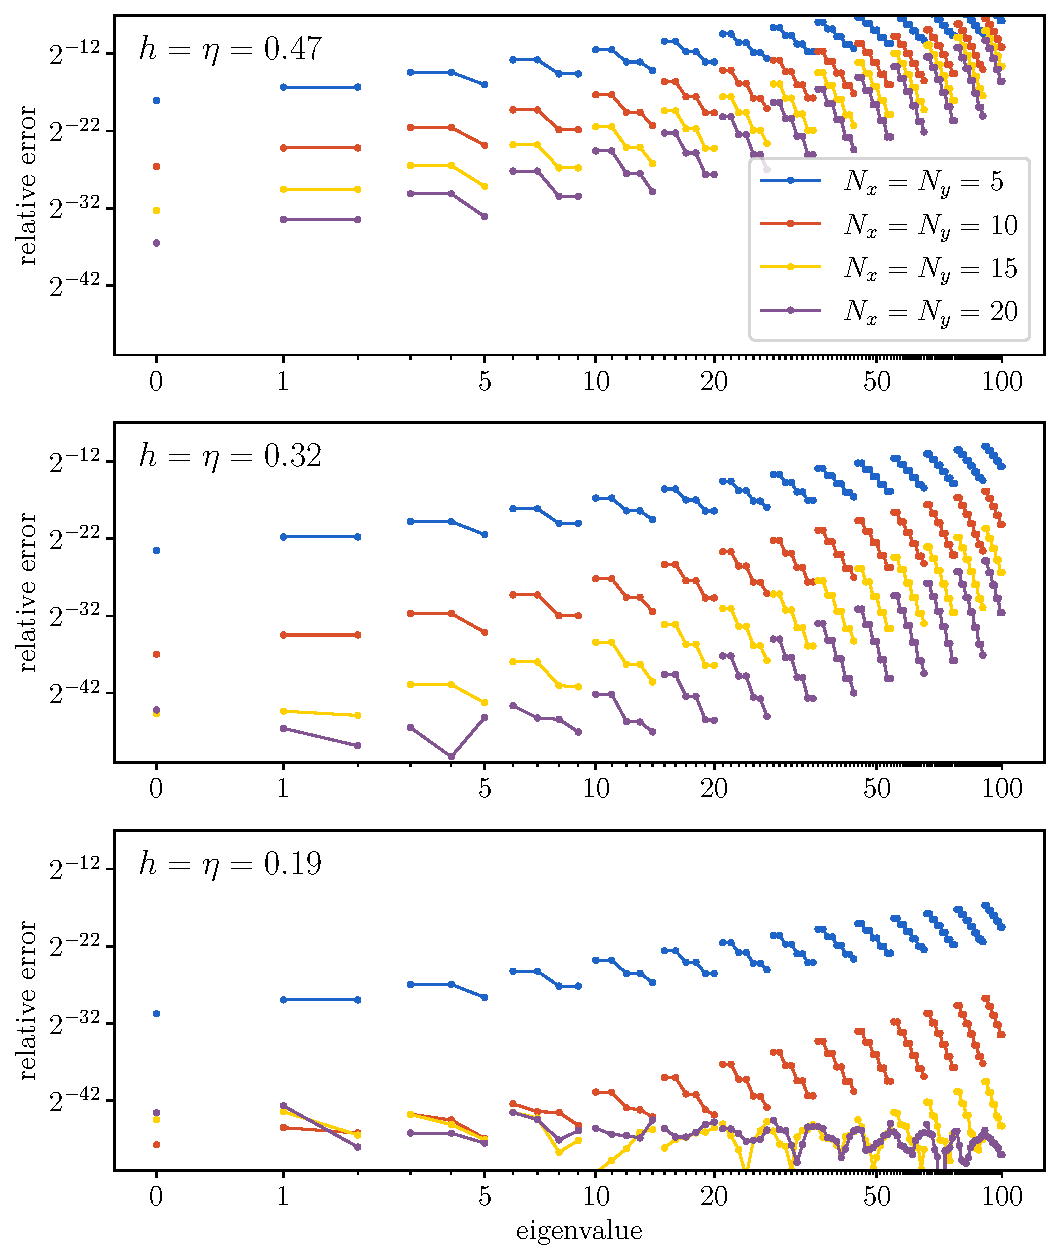
\includegraphics[width=\textwidth]{img/chapter4/fd_harmonic.pdf}
    \end{center}
    \caption{These graphs display the relative error of each of the first $100$ eigenvalues of the harmonic oscillator \eqref{equ:c4_fd_harmonic}, computed for different values of $h = \eta$ and $N_x = N_y$. Repeated eigenvalues are connected.}
    \label{fig:c4_fd_harmonic}
\end{figure}

As a first example we will replicate the results of \cite{wang_new_2009} for the harmonic oscillator:
\begin{equation}\label{equ:c4_fd_harmonic}
    -\nabla^2 \psi(x, y) + \left(x^2 + y^2\right) \psi(x, y) = E \psi(x, y)
\end{equation}
on the domain $[\numprint{-9.5}, \numprint{9.5}] \times [\numprint{-9.5}, \numprint{9.5}]$ with homogeneous Dirichlet boundary conditions. Notice that in \cite{wang_new_2009} the authors have chosen to scale the potential and eigenvalue by an extra factor of two. Here we did not do this, as such are computed eigenvalues will be twice as large. But, the relative errors remain the same.

In figure \ref{fig:c4_fd_harmonic} the relative errors for the first $100$ eigenvalues are plotted. This is done for $h = \eta \in \left\{\frac{19}{40}, \frac{19}{60}, \frac{19}{100}\right\}$ and $N_x = N_y \in \left\{ 5, 10, 20, 25 \right\}$. In these graphs a few things can be noted. Unsurprisingly, when $N_x = N_y$ is increased, the results become more accurate. And also, when $h = \eta$ is decreased, that is to say more grid points are used, the results also become more accurate. As is the case with most algorithms for approximating Schrödinger equations, when larger eigenvalues are computed, the accuracy decreases. The corresponding eigenfunctions become more and more oscillatory, and are thus more difficult to approximate accurately.

But most impressively, all these graphs were computed within a minute on a simple laptop. More detailed runtime analysis can be found in section \ref{sec:c4_nm_vs_fd}. Furthermore, the obtained results are also impressive. In the most accurate case $h= \eta = \frac{19}{100}$ and $N_x = N_y = 20$, the first $100$ eigenvalues are found with $45$ bits of precision, which is close to the ideal machine precision of $53$ bits.

To get a deeper understanding of this finite difference method it may be beneficial to study the asymptotic behavior of the error, with respect to the number of discretization points and the index of the eigenvalue. The finite difference approximation error can be used as a jumping point. Assume $N = N_x = N_y$, then the finite difference approximation of the second derivative of a function $f : \RR \to \RR$ is of the form:
$$
    f''(x) = \frac{1}{h^2}\sum_{i=-N}^{N} c_{i} f(x + i h) + \OO\mleft(h^{2N}\mright)\text{.}
$$

Going further with a theoretical analysis becomes unnecessarily difficult. We will estimate the order by using the numerical results for the first $100$ eigenvalues of the harmonic oscillator, calculated for the values of $h = \eta = \frac{1}{n}$ for $n \in \left\{20, 30, 40, 50, 60, 70, 80, 90, 100\right\}$. These $9$ different sets of parameters yield for each of the $100$ eigenvalues (with index $k \in \{1, 2, \dots, 100\}$) a data point. Next, through all these points we find the best fitting curve which follows the formula $\alpha_1 h^{\alpha_2} k^{\alpha_3}$. In this case we define the best fitting curve to be such that for the error $\epsilon_k^{(h)}$ (for each eigenvalue $k$ calculated with a step size of $h = \eta$), the following is minimized:
$$
    \sum_{k, h}\left|\log|\epsilon_{k}^{(h)}| - \log\mleft(c_1 h^{c_2} k^{c_3}\mright)\right|^2 \text{.}
$$

These best fits are summarized in the following table.
\begin{center}
    \begin{tabular}{r|cccc}
$N_x = N_y$ & $5$ & $10$ & $15$ & $20$ \\\hline\rule{0pt}{2.6ex}
Error & $\OO\mleft(h^{\numprint{3.90}}k^{\numprint{2.96}}\mright)$ & $\OO\mleft(h^{\numprint{5.78}}k^{\numprint{2.92}}\mright)$ & $\OO\mleft(h^{\numprint{6.61}}k^{\numprint{2.86}}\mright)$ & $\OO\mleft(h^{\numprint{7.07}}k^{\numprint{2.83}}\mright)$
\end{tabular}

\end{center}

It is important to note that these values are estimates, and are quite sensitive to the used values of $n$ and $k$. But, some trends are visible. We first note that increasing $N$ indeed increases the order in $h$ as well, maybe not as much as theoretical assumed $\OO\mleft(h^{2N}\mright)$, but nonetheless significantly. One of the reasons this theoretical value of $h^{2N}$ is not reached is because of the limited precision available in the \texttt{double} floating point type. For low eigenvalues, larger grids, and higher values of $N$, the error is so small that the numerical precision of the datatype becomes the main source of error. Another visible behavior is that a more accurate (higher order in $h$) method also has a larger exponent with respect to $k$. This means that higher eigenvalues are asymptotically less accurate. This property can also be seen in the graphs of figure \ref{fig:c4_fd_harmonic}, a virtual line through the points corresponding to $N = 5$ is less steep than a line through the points of $N = 10$.

For one-dimensional problems the behavior of the error with respect to $k$ has already been well studied and improved. In \cite{paine_correction_1981} expressions are constructed which provide a correction to the numeric approximation with a finite difference scheme for Sturm-Liouville problems. These correction formulae bring the order in $k$ down from $\OO(k^4h^2)$ to $\OO(k h^2)$. For multidimensional Schrödinger equations no such corrections are available, let alone for the extremely high order schemes considered here.

\paragraph{Zero potential} Besides the harmonic oscillator it is also instructive to consider the problem with a zero potential function on the domain $\Omega = [0, \pi] \times [0, \pi]$ and homogeneous Dirichlet boundary conditions. So, find all eigenvalues $E$ for which there exists an eigenfunction $\psi(x, y)$ on the domain with $\psi(x, y) = 0$ on $\dOmega$ such that the following holds:
\begin{equation}\label{equ:c4_fd_zero}
    -\nabla^2 \psi(x, y) = E \psi(x, y) \text{.}
\end{equation}

\begin{figure}
    \begin{center}
        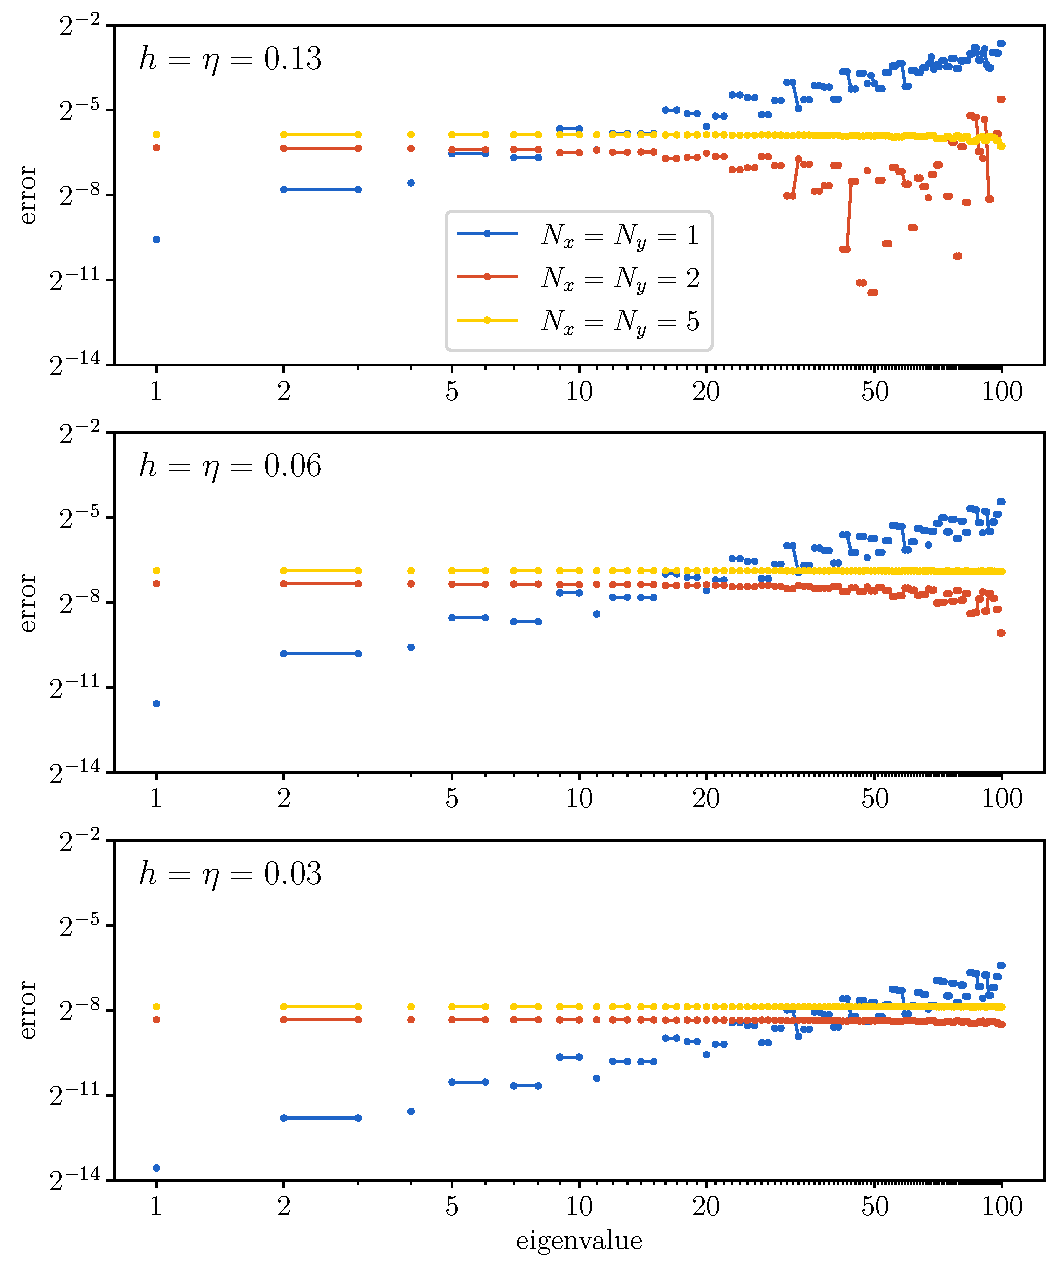
\includegraphics[width=\textwidth]{img/chapter4/fd_zero.pdf}
    \end{center}
    \caption{These graphs display the relative error of each of the first $100$ eigenvalues of a Schrödinger problem with a zero potential on the rectangular $[0, \pi] \times [0, \pi]$ domain with homogeneous Dirichlet boundary conditions \eqref{equ:c4_fd_zero}. This error is computed for different values of $h = \eta$ and $N_x = N_y$. Repeated eigenvalues are connected.}
    \label{fig:c4_fd_zero}
\end{figure}

By separation of variables, the exact solutions of this equation can be found: $\psi_{i, j}(x, y) = \sin(i x)\sin(j y)$ with eigenvalue $\lambda_{i,j} = i^2 + j^2$ for all $i, j \in \Nplus$. The first few of these eigenvalues are listed.
\begin{align*}
\lambda_{1,1} &= 2 & \lambda_{3,3} &= 18 & \lambda_{3,5} = \lambda_{5,3} &= 34\\
\lambda_{1,2} = \lambda_{2,1} &= 5 & \lambda_{2,4} = \lambda_{4,2} &= 20 & \lambda_{1,6} = \lambda_{6,1} &= 37\\
\lambda_{2,2} &= 8 & \lambda_{3,4} = \lambda_{4,3} &= 25 & \lambda_{2,6} = \lambda_{6,2} &= 40\\
\lambda_{1,3} = \lambda_{3,1} &= 10 & \lambda_{1,5} = \lambda_{5,1} &= 26 & \lambda_{4,5} = \lambda_{5,4} &= 41\\
\lambda_{2,3} = \lambda_{3,2} &= 13 & \lambda_{2,5} = \lambda_{5,2} &= 29 & \lambda_{3,6} = \lambda_{6,3} &= 45\\
\lambda_{1,4} = \lambda_{4,1} &= 17 & \lambda_{4,4} &= 32 & \lambda_{1,7} = \lambda_{5,5} = \lambda_{7,1} &= 50
\end{align*}%

In a certain way, these eigenvalues are more interesting than those from the harmonic oscillator, as their multiplicities are less predictable.

In figure \ref{fig:c4_fd_zero} the relative error in each of the first $100$ eigenvalues is displayed for different values of $h = \eta$ and $N_x = N_y$. When comparing this figure to the results of the harmonic oscillator \ref{fig:c4_fd_harmonic}, some striking differences can be seen. Maybe most surprisingly, increasing the order does not give more accurate results! For low eigenvalues the method with $N_x=N_y=1$ is most accurate, this is simply the second order central finite difference formula. When using higher order methods the error does not get any better than $2^{-8}\approx \numprint{0.00391}$, which is not at all as accurate as the results for the harmonic oscillator, where the error for $N_x=N_y = 5$ lies between $2^{-32} \approx \numprint{2.3e-10}$ and at most $2^{-16} \approx \numprint{1.5e-05}$. This is quite a disconcerting behavior for a numerical method to have.

These results bring to light one of the biggest drawbacks of the method from \cite{wang_new_2009}. This method only works if it is assumed that the eigenfunctions always are zero outside the domain. For the harmonic oscillator, this is the case, as $V(x, y) \to +\infty$ if $\|x, y\| \to +\infty$. For the zero potential function this is definitely not the case, the eigenfunctions are periodic. One could argue that, in theory, an eigenfunction may be anything outside the domain $\Omega$. So in particular, we could define them to be zero there. But, most numerical methods, and this method in particular, assume that solutions are sufficiently continuous. To cleanly define the problem, at least $C_0^2(\Omega)$ is needed, and when using $N^\text{th}$ order central finite difference schemes are used $C_0^{N}(\Omega)$ is implicitly assumed. And this assumption fails if we define the function to be zero outside $\Omega$.

To combat this issue, on the boundary of the domain asymmetric schemes could be used, the authors of \cite{wang_new_2009} did not do this. As an example, we have tabulated all relevant seven point formulae.
\begin{center}
    \begin{tabular}{ccc|c|ccccc|r}
$c_{-3}$ & $c_{-2}$ & $c_{-1}$ & $c_{0}$ & $c_{1}$ & $c_{2}$ & $c_{3}$ & $c_{4}$ & $c_{5}$ & error \\\hline
\rule{0pt}{3ex} $\frac{1}{90}$ & $- \frac{3}{20}$ & $\frac{3}{2}$ & $- \frac{49}{18}$ & $\frac{3}{2}$ & $- \frac{3}{20}$ & $\frac{1}{90}$ &  &  & $\OO\mleft(h^{6}\mright)$ \\
\rule{0pt}{3ex}  & $- \frac{13}{180}$ & $\frac{19}{15}$ & $- \frac{7}{3}$ & $\frac{10}{9}$ & $\frac{1}{12}$ & $- \frac{1}{15}$ & $\frac{1}{90}$ &  & $\OO\mleft(h^{5}\mright)$ \\
\rule{0pt}{3ex}  &  & $\frac{137}{180}$ & $- \frac{49}{60}$ & $- \frac{17}{12}$ & $\frac{47}{18}$ & $- \frac{19}{12}$ & $\frac{31}{60}$ & $- \frac{13}{180}$ & $\OO\mleft(h^{5}\mright)$ \\
\end{tabular}

\end{center}
There are two difficulties when using these formulae. Firstly, to reach the required order, one point more should be used. And secondly, when using asymmetric formulae the matrix from \eqref{equ:c4_fd_sparse_matrix} looses its symmetry as well. In principle this should not matter. But, in practice, many sparse matrix eigenvalue solvers are much more efficient when working with a real symmetric matrix.

    {\color{red}To do: give some results of this extension, maybe in a later subsection}

\paragraph{Hénon-Heiles} Lastly, ... {\color{red}To do}


\subsubsection{Computational cost of the method}

Finite differences are employed in many real-world applications, as they are easy to implement, yet are able to reach high accuracies. In practice, however, it is rare to see these very high orders used. In this setting these high orders seem to be very well applicable.

Yet, these finite difference methods are not without issues. One of the most prominent drawbacks is the expensive computations involved. To get accurate results, high orders combined with fine grids have to be used. This results in huge sparse matrices. And only thanks to their sparsity are algorithms able to compute the eigenvalues. Now, for higher order schemes, the matrices become less sparse, and as such more expensive to work with.

Alternatively, a method which is able to reduce the size of the matrices involved without losing accuracy may be preferable.

\subsection{A semi-discrete method}\label{sec:c4_semi_discrete}

{\color{red} To do: consider writing this intermediate method}

\section{A woven interpolation method}

In contrast to the previous methods, we propose a technique which is not necessarily restricted to cases where the domain is only a rectangle. So consider a finite domain $\Omega \subseteq \RR^2$ on which we are searching for eigenvalues $E \in \RR$ and eigenfunctions $\psi: \Omega \to \RR$ such that for a given potential $V : \Omega \to \RR$ the following holds
\begin{equation}\label{equ:c4_schrodinger_equation_new_method}
    -\nabla^2 \psi + V(x, y) \psi = E \psi\text{.}
\end{equation}
Still, we impose homogeneous Dirichlet boundary conditions: $\psi(x, y) = 0$ for $(x, y) \in \Omega$.

The main idea underlying this method is that we want to represent the eigenfunctions $\psi$ efficiently. A fully discretized method may represent eigenfunctions as its values on certain grid points. Our first attempt to develop a more continuous approximation of the eigenfunction used ideas from chapter \ref{cha:c3} and led to the creation of section \ref{sec:c4_semi_discrete}, where we have chosen to approximate the eigenfunction as a linear combination of well-chosen basis functions on parallel lines throughout the domain. This led to a continuous approximation along one direction and a discrete approximation along the other direction of the domain.

\begin{figure}
    \begin{center}
        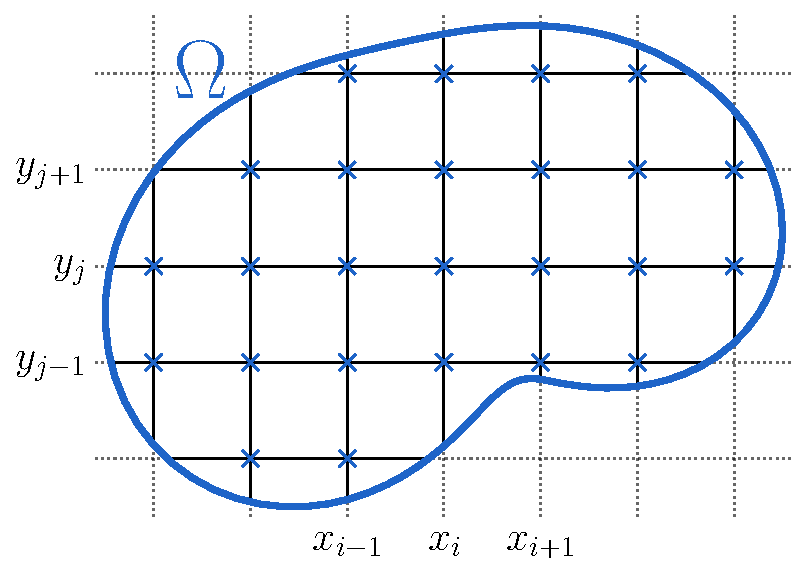
\includegraphics[width=.66\linewidth]{img/chapter4/the_method_grid.pdf}
        \caption{\label{fig:woven_method_grid} The grid}
    \end{center}
\end{figure}

We are now going to construct a new method in which we will bring this continuous approximation to both directions of the domain. For this, we place a grid over the domain $\Omega$, as can be seen in figure \ref{fig:woven_method_grid}. This grid does not need to be equidistant. When developing this new method we strived to allow for maximal flexibility, by avoiding as many restrictions on $\Omega$ as possible. This has as consequence that, because $\Omega$ does not have to be a rectangle, the number of intersections per grid line is not necessarily constant. Even worse, because we do not even require $\Omega$ to be convex, the intersection of a grid line with $\Omega$ may not be continuous. Upon formulating and implementing this new method, this varying number of intersections and these noncontinuous grid lines are some example of difficulties that arise by explicitly allowing more flexibility.

After placing the grid on $\Omega$, the next step is to approximate the unknown eigenfunction $\psi$ as a linear combination of basis functions on each of the grid lines. On the vertical line $x = x_i$, we denote these basis functions as $\beta_k^{(x_i)}(y)$, for each value of $k$. This yields the expression
\begin{equation}\label{equ:c4_expression_on_lines_x}
    \psi(x_i, y) = \sum_{k=0}^\infty c_k^{(x_i)} \beta_k^{(x_i)}(y) \text{.}
\end{equation}

For horizontal lines $y = y_j$, the basis functions $\beta_k^{(y_j)}(x)$ yield a similar expression
\begin{equation}\label{equ:c4_expression_on_lines_y}
    \psi(x, y_j) = \sum_{k=0}^\infty c_k^{(y_j)} \beta_k^{(y_j)}(x) \text{.}
\end{equation}

Notice that the domain of each of these $\beta$-fucntions is the intersection of its corresponding grid line with $\Omega$. As earlier stated, this domain may not be continuous. In theory this is not a problem, as long as the definition of $\beta$ allows this. And, it will. In practice when one wants to implement this, care has to be taken. It may be beneficial to construct multiple separate sets of basis functions for each of the continuous parts of the grid line. Because the theory has no problem with discontinuities, we will not burden the notation and explanation with this separation into continuous parts.

To ensure $\psi(x, y)$ is uniquely defined in each point in $\Omega$ we have to require that in each intersection point $(x_i, y_j)$, $\psi(x_i, y_j)$ has only one solution:
\begin{equation}\label{equ:c4_new_method_pre_matrix_equality}
    \psi(x_i, y_j) = \sum_{k=0}^\infty c_k^{(x_i)} \beta_k^{(x_i)}(y_j) = \sum_{k=0}^\infty c_k^{(y_j)} \beta_k^{(y_j)}(x_i)\text{.}
\end{equation}

Before deciding on which basis functions we should use, let us consider the Schrödinger equation \eqref{equ:c4_schrodinger_equation_new_method} on each intersection point $(x_i, y_j)$ with this new representation of $\psi$:
$$
    -\sum_{k=0}^\infty c_k^{(x_i)} \beta''^{(x_i)}_k(y_j) - \sum_{k=0}^\infty c_k^{(y_j)} \beta''^{(y_j)}_k(x_i) + (V(x_i, y_j) - E) \psi(x_i, y_j) = 0\text{.}
$$

This last formula suggest choosing $\beta_k^{(x_i)}$ and $\beta_k^{(y_j)}$, such that its second derivative contains, in a certain sense, $V(x_i, y_j)$. Together with the idea from chapter \ref{cha:c3} to use a one-dimensional Schrödinger equation, this leads us to propose $\beta_k^{(x_i)}$ to be the ordered eigenfunctions which satisfy the one dimensional Schrödinger equation
$$
    -\beta_k''^{(x_i)}(y) + \frac{V(x_i, y)}{2}\beta_k^{(x_i)}(y) = \lambda_k^{(x_i)} \beta_k^{(x_i)}(y)
$$
with homogeneous Dirichlet boundary conditions. The domain for this one-dimensional problem is the intersection of the vertical line $x = x_i$ and the two-dimensional domain $\Omega$. Similarly, for the horizontal line $y = y_j$, we propose $\beta_k^{(y_j)}(x)$ to be the eigenfunctions of
$$
    -\beta_k''^{(y_j)}(x) + \frac{V(x, y_j)}{2}\beta_k^{(y_j)}(x) = \lambda_k^{(y_j)} \beta_k^{(y_j)}(x)
$$
with homogeneous Dirichlet boundary conditions, and as domain the intersection of $y = y_j$ and $\Omega$.

By choosing half the original potential in each of the approximations, in each intersection $(x_i, y_j)$, equation \eqref{equ:c4_schrodinger_equation_new_method} simplifies, and $V(x, y)$ disappears:
\begin{equation}\label{equ:c4_new_method_pre_matrix}
    \sum_{k=0}^\infty \lambda_k^{(x_i)} c_k^{(x_i)} \beta^{(x_i)}_k(y_j) + \sum_{k=0}^\infty \lambda_k^{(y_j)} c_k^{(y_j)} \beta_k^{(y_j)}(x_i) = E \psi(x_i, y_j) \text{.}
\end{equation}

Notice that in this expression only $E$ (the eigenvalue) and $c_k^{(x_i)}$ and $c_k^{(y_j)}$ are unknown, as $\psi(x_i, y_j)$ depends linearly on $c_k^{(x_i)}$ and $c_k^{(y_j)}$. So, expression \eqref{equ:c4_new_method_pre_matrix} is, in fact, a linear problem.

Before writing this as a matrix-problem, we first have to limit the extent of the sum. It is, of course, impossible to implement these formulas while the function bases are still infinite. Therefor, we limit the basis on the line $x = x_i$ to the first $K_{x_i}$ functions and to the first $K_{y_j}$ functions on the line $y = y_j$. Notice that the size of a basis on each line, should not be greater than the number of intersections on that line. If the basis size is too large, the system \eqref{equ:c4_new_method_pre_matrix_equality} would be underdetermined. In this case, solutions will no longer be uniquely defined, which is a problem. In contrast, if the basis size is smaller, the system \eqref{equ:c4_new_method_pre_matrix_equality} would be overdetermined. This does not lead to issues, because we can reformulate it as finding solutions in a least squares sense.

With these finite sums equations \eqref{equ:c4_new_method_pre_matrix_equality} and \eqref{equ:c4_new_method_pre_matrix} become, on the intersection $(x_i, y_j)$:
\begin{align}
     & \sum_{k=0}^{K_{x_i}-1} \lambda_k^{(x_i)} c_k^{(x_i)} \beta^{(x_i)}_k(y_j) + \sum_{k=0}^{K_{y_j}-1} \lambda_k^{(y_j)} c_k^{(y_j)} \beta_k^{(y_j)}(x_i)\nonumber                                  \\
     & \qquad\qquad\qquad     = \sum_{k=0}^{K_{x_i}-1} c_k^{(x_i)} \beta_k^{(x_i)}(y_j) = \sum_{k=0}^{K_{y_j}-1} c_k^{(y_j)} \beta_k^{(y_j)}(x_i) \text{.}\label{equ:c4_new_method_pre_matrix_unified}
\end{align}
The introduction of appropriate vectors and matrices will allow us to translate \eqref{equ:c4_new_method_pre_matrix_unified} into a matrix problem. The unknowns will be summarized into the two vectors $\vb{c_x}$ and $\vb{c_y}$, with sizes $n_x := \sum_i K_{x_i}$ and $n_y := \sum_j K_{y_j}$ respectively:
\begin{align*}
    \vb{c_x}            & = \transpose{\begin{pmatrix} c_0^{(x_0)} & c_1^{(x_0)} & \dots & c_{K_{x_0}-1}^{(x_0)} & c_0^{(x_1)} & c_1^{(x_1)} & \dots \end{pmatrix}}         \\
    \text{and }\vb{c_y} & = \transpose{\begin{pmatrix} c_0^{(y_0)} & c_1^{(y_0)} & \dots & c_{K_{y_0}-1}^{(y_0)} & c_0^{(y_1)} & c_1^{(y_1)} & \dots \end{pmatrix}}\text{.}
\end{align*}

Furthermore, we introduce the $n_x \times n_x$ diagonal matrix $\vb{\Lambda_x}$ and the $n_y \times n_y$ diagonal matrix $\vb{\Lambda_y}$ which contain the eigenvalues of the one-dimensional Schrödinger problems used to define the basis functions:
\begin{align*}
    \vb{\Lambda_x}            & = \diag\begin{pmatrix} \lambda_0^{(x_0)} & \lambda_1^{(x_0)} & \dots & \lambda_{K_{x_0}-1}^{(x_0)} & \lambda_0^{(x_1)} & \lambda_1^{(x_1)} & \dots \end{pmatrix}         \\
    \text{and }\vb{\Lambda_y} & = \diag\begin{pmatrix} \lambda_0^{(y_0)} & \lambda_1^{(y_0)} & \dots & \lambda_{K_{y_0}-1}^{(y_0)} & \lambda_0^{(y_1)} & \lambda_1^{(y_1)} & \dots \end{pmatrix}\text{.} \\
\end{align*}

\begin{figure}
    \begin{center}
        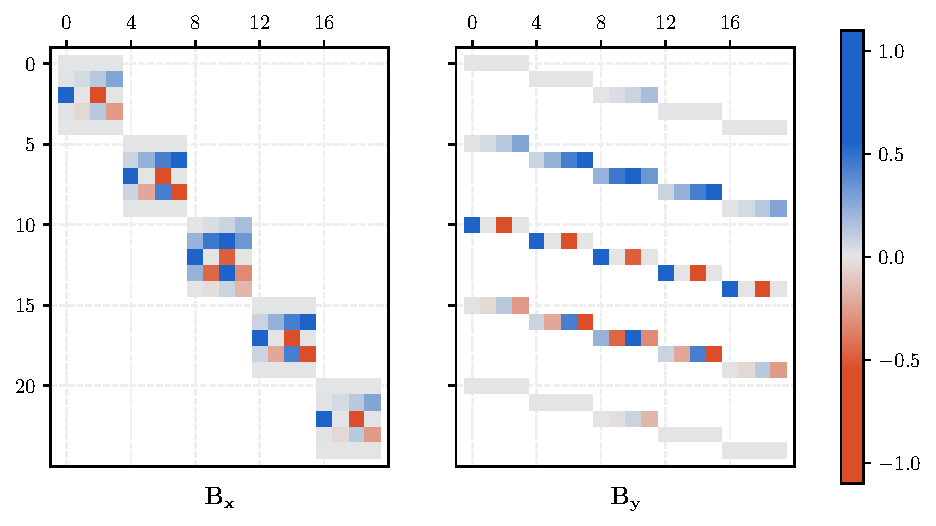
\includegraphics[width=\textwidth]{img/chapter4/new_method_beta.pdf}
        \caption{The non-zero entries of the matrices $\vb{B_x}$ and $\vb{B_y}$ from equation \eqref{equ:c4_new_method_beta_definition} are visualized. These were calculated on the problem from section \ref{sec:c4_numerical_ixaru} with a 5 by 5 internal grid and $K_{x_i} = K_{y_j} = 4$ basis functions per line. In practice, these matrices are much larger.}
        \label{fig:c4_new_method_beta}
    \end{center}
\end{figure}

Lastly we define the matrices which contain the values of the basis functions in each of the grid points. For this let us define $m$ as the total number of intersection points. Now, we define the $m \times n_x$ matrix $\vb{B_x}$ and the $m \times n_y$ matrix $\vb{B_y}$. Each row $r_{i,j}$ of these matrices correspond to a grid point $(x_i, y_j)$. The non-zero entries on each of the rows $r_{i,j}$ of the matrices $\vb{B_x}$ and $\vb{B_y}$ can be calculated as
\begin{align}
    \left(\vb{B_x}\right)_{r_{i,j}, o^{(x)}_{i} + k} & =  \beta_{k}^{(x_i)}(y_j) \text{ for $k \in \{0, 1, \dots, K_{x_i} - 1\}$ }   \nonumber                               \\
    \text{and }
    \left(\vb{B_y}\right)_{r_{i,j}, o^{(y)}_{j} + k} & =  \beta_{k}^{(y_j)}(x_i) \text{ for $k \in \{0, 1, \dots, K_{y_i} - 1\}$.} \label{equ:c4_new_method_beta_definition}
\end{align}
In this expression the values $o^{(x)}_{i}$ and $o^{(y)}_{j}$ are certain offsets depending on the row. These offsets are defined as: $o^{(x)}_{i} := \sum_{i' < i} K_{x_{i'}}$ and $o^{(y)}_{j} := \sum_{j' < j} K_{y_{j'}}$. To aid an intuitive understanding of the $\vb{B_x}$ and $\vb{B_y}$ matrices, figure \ref{fig:c4_new_method_beta} provides a schematic view of them, calculated from a small numerical example.

As promised, these definitions allow us to rewrite the system \eqref{equ:c4_new_method_pre_matrix_unified} with $m$ equations more compactly as:
\begin{equation}\label{equ:c4_nm_matrix_compact}
    \vb{B_x} \vb{\Lambda_x}\vb{c_x} + \vb{B_y} \vb{\Lambda_y}\vb{c_y} = E \vb{B_x} \vb{c_x} = E \vb{B_y} \vb{c_y}\text{.}
\end{equation}

This formulation is not yet reminiscent of any classical linear algebra problem. One of the unfamiliar parts of this expression is the fact that there are two vectors of unknowns, another unfamiliar part is that \eqref{equ:c4_nm_matrix_compact} defines, in fact, two different equations.
\begin{equation}
    \begin{cases}
        \vb{B_x} \vb{\Lambda_x}\vb{c_x} + \vb{B_y} \vb{\Lambda_y}\vb{c_y} = E \vb{B_x} \vb{c_x} \\
        \vb{B_x} \vb{c_x} = \vb{B_y} \vb{c_y}
    \end{cases} \label{equ:c4_new_method_first_matrix_problem}
\end{equation}

There are a few strategies to further translate this problem into a form for which efficiently implemented and well-studied algorithms exist. Ideally, the solution would take the sparsity of the involved matrices into account.

\subsection{Solving the matrix approximation}

As a first strategy we investigated how this problem can be directly transformed into a standard mathematical problem.

\subsubsection{Direct transformation into an eigenvalue problem}

We tackle equation \eqref{equ:c4_new_method_first_matrix_problem} by rewriting it as
$$
    \begin{cases}
        \vb{B_x} \vb{\Lambda_x}\vb{c_x} + \vb{B_y} \vb{\Lambda_y}\vb{c_y} = E \vb{B_x} \vb{c_x} \\
        \vb{B_x} \vb{\Lambda_x}\vb{c_x} + \vb{B_y} \vb{\Lambda_y}\vb{c_y} = E \vb{B_y} \vb{c_y} \\
    \end{cases}\text{.}
$$
This system can be seen as the following generalized rectangular eigenvalue problem:
\begin{equation}\label{equ:c4_new_method_alternative_system}
    \begin{pmatrix}
        \vb{B_x} \vb{\Lambda_x} & \vb{B_y} \vb{\Lambda_y} \\
        \vb{B_x} \vb{\Lambda_x} & \vb{B_y} \vb{\Lambda_y}
    \end{pmatrix} \begin{pmatrix}
        \vb{c_x} \\ \vb{c_y}
    \end{pmatrix} = E \begin{pmatrix}
        \vb{B_x} & \vb{0} \\ \vb{0} & \vb{B_y}
    \end{pmatrix} \begin{pmatrix}
        \vb{c_x} \\ \vb{c_y}
    \end{pmatrix}\text{.}
\end{equation}

At first glance this may seem to enable us to solve the problem elegantly. But, there are a few issues apparent with this translation. One of the most visible problems is that we have translated this into a matrix problem which is twice as large as the original matrices $\vb{B_x}$ and $\vb{B_y}$ in both rows and columns. On the other hand, one can argue that the matrices are clearly sparse. The matrices $\vb{B_x}$ and $\vb{B_y}$ are sparse indeed, but the problem is that there are few algorithms available that are even able to solve a generalized rectangular eigenvalue problem, let alone a sparse one.

But a lack of sparse implementations does not deter us from trying out some numerical experiments. In this first experiment we will have to fall back to algorithms working on dense matrices. Of course, the runtime will suffer, but from a numerical point of view the results will still be valuable.

Consider the Schrödinger equation with the harmonic oscillator potential:
$$
    -\nabla^2\psi(x, y) + \left(x^2 + y^2\right) \psi(x, y) = E \psi(x, y)
$$
on the domain $[-9.5, 9.5] \times [-9.5, 9.5]$ with homogeneous Dirichlet boundary conditions\footnote{We also considered this problem in section \ref{sec:c4_fd_numerical}.}. We apply the described method on a grid with 30 lines in each direction and 16 basis functions per line. This yields $900\times 480$ matrices $\vb{B_x}$ and $\vb{B_y}$, and the rectangular problem from \eqref{equ:c4_new_method_alternative_system} has \numprint{1800} equations and \numprint{960} variables. As this eigenvalue problem is heavily overdetermined, we have to considered that solutions will only be accurate in a least squares sense. Much research is already dedicated to solving this kind of problem, as such we will, for now, use the first method from \cite{hua_svd_1991} to find solutions. Later on, we will explore the world of generalized rectangular eigenvalue problems.

If we write equation \eqref{equ:c4_new_method_alternative_system} symbolically as $\vb{A} \vb{c} = E \vb{D} \vb{c}$, and the truncated singular value decomposition of $\vb{D}$ as $\vb{D} = \vb{U_D} \vb{\Sigma_D} \vb{V_D^\adjointsign}$, then any solution of \eqref{equ:c4_new_method_alternative_system} will also be a solution of the generalized square eigenvalue problem
$$
    \vb{U_D^\adjointsign} \vb{A} \vb{V_D} \vb{v} = E \vb{\Sigma_D} \vb{v} \text{,}
$$
with $\vb{c} = \vb{V_D} \vb{v}$. Applying this method to the numerical problem yields 840 eigenvalues. Firstly, it is important to remark that the resulting values are elements of $\CC$. But, in this case, the imaginary part of all values lies between \numprint{-1.68e-14} and \numprint{1.68e-14}, so all values may be considered real. The lowest few values are given:
$$
    \underbrace{
        \numprint{-2.85e-14} \quad \dots \quad \numprint{5.39e-14}
    }_\text{256 values close to zero} \quad \numprint{2.00} \quad \numprint{3.93} \quad \numprint{3.93} \quad \numprint{4.00} \quad \numprint{4.00} \quad \dots
$$

This can be more compactly summarized when the number of times an eigenvalue is (up to a precision of $10^{-6}$) repeated is indicated by a subscript:

\begin{tabular}{ccccccccccc}
    $\numprint{0.00}_{256}$ & $\numprint{2.00}$ & $\numprint{3.93}_2$ & $\numprint{4.00}_2$ & $\numprint{5.36}_2$ & $\numprint{6.00}_3$ & $\numprint{6.78}_2$ & $\numprint{6.87}_2$ & $\numprint{8.00}_4$ & $\dots$
\end{tabular}

One immediately notices the many returned zero values. Some of these can be explained by the structure of the matrix on the left-hand size of \eqref{equ:c4_new_method_alternative_system}. This is a $2\cdot 900 \times (480 + 480)$ matrix with repeated rows. The rank is thus at most $900$, which explains $960 - 900 = 60$ zero eigenvalues. The others are more difficult to explain, but suggestions can be found in the fact that $\vb{B_x} \vb{\Lambda_x} \vb{c_x}$ and $\vb{B_y} \vb{\Lambda_y} \vb{c_y}$ describe (up to a least squares approximation) the same points. So, $\vb{c_x}$ and $\vb{c_y}$ are not independent, which implies that the rank of the matrix $\begin{pmatrix} \vb{B_x} \vb{\Lambda_x} & \vb{B_y} \vb{\Lambda_y}\end{pmatrix}$ will probably not be maximal. But, these zero eigenvalues indicate another problem. Namely, that for these values it is not at all guaranteed that $\vb{B_x} \vb{c_x} = \vb{B_y} \vb{c_y}$. So, these eigenvalues will be nonsensical in the context of the original Schrödinger problem.

Remember that the true eigenvalues of the harmonic oscillator are 2, 4, 4, 6, 6, 6, 8, 8, 8, 8, \dots. And, we notice that these true values can indeed be found in our solutions, but also many other values are present. Because the method from \cite{hua_svd_1991} for solving generalized rectangular eigenvalue problems may return more solutions than the original problems has, we still have to filter some out. One way to only end up with true eigenvalues is by substituting them back into the original problem \eqref{equ:c4_new_method_first_matrix_problem} and verifying the residuals of both equations:
$$
    r_1 = \left\| \vb{B_x} \vb{\Lambda_x} \vb{c_x} + \vb{B_y} \vb{\Lambda_y} \vb{c_y} - \frac{E}{2}\left(\vb{B_x}\vb{c_x} + \vb{B_y}\vb{c_y}\right) \right\| \text{ and } r_2=\left\| \vb{B_x} \vb{c_x} - \vb{B_y} \vb{c_y} \right\|\text{.}
$$

The found possible eigenvalue with the lowest residuals $r_1$ and $r_2$ are also true eigenvalues of the Schrödinger problem. When we sort all possibilities by their first residual $r_1$ we obtain the following table.

\begin{center}
    \begin{tabular}{r|rrrrr}
$E$ & \numprint{2.000000} & \numprint{4.000000} & \numprint{4.000000} & \numprint{6.000000} & \numprint{7.999998} \\\hline
$r_1$ & \numprint{1.5e-5} & \numprint{4.7e-4} & \numprint{4.7e-4} & \numprint{4.9e-4} & \numprint{5.0e-3} \\
$r_2$ & \numprint{1.2e-5} & \numprint{2.3e-4} & \numprint{2.3e-4} & \numprint{1.6e-4} & \numprint{1.2e-3}
\end{tabular}

\begin{tabular}{r|rrrrr}
$E$ & \numprint{7.999998} & \numprint{9.999997} & \numprint{9.999997} & \numprint{10.000006} & \numprint{8.000007} \\\hline
$r_1$ & \numprint{5.0e-3} & \numprint{6.6e-3} & \numprint{6.7e-3} & \numprint{1.0e-2} & \numprint{1.4e-2} \\
$r_2$ & \numprint{1.2e-3} & \numprint{1.3e-3} & \numprint{1.3e-3} & \numprint{2.1e-3} & \numprint{3.5e-3}
\end{tabular}

\begin{tabular}{r|rrrrr}
$E$ & \numprint{8.000007} & \numprint{13.999988} & \numprint{5.999974} & \numprint{5.999974} & \numprint{10.000151} \\\hline
$r_1$ & \numprint{1.4e-2} & \numprint{1.9e-2} & \numprint{3.8e-2} & \numprint{3.8e-2} & \numprint{4.8e-2} \\
$r_2$ & \numprint{3.5e-3} & \numprint{2.7e-3} & \numprint{1.3e-2} & \numprint{1.3e-2} & \numprint{9.6e-3}
\end{tabular}


\end{center}

Here, we see that when the first residual $r_1$ is low, the other is as well. Also, in the first few eigenvalues, only true solutions are present.

Upon studying this direct method to solve the system of equations \eqref{equ:c4_new_method_first_matrix_problem}, we have noticed some drawbacks. Firstly, the proposed system \eqref{equ:c4_new_method_alternative_system} is, in a certain sense, twice as large as the discrete problem we started from. Eigenvalue algorithms are at least cubic in complexity. So, this doubling in size implies an eightfold runtime penalty. Secondly, and numerically interesting, we obtain many more `solutions' than the ones we are looking for. Each generalized eigenvalue, with its eigenvector, has to be computed and checked against the residuals. Many eigenvalues will be thrown away.

\subsubsection{Restriction to a null space}\label{sec:nm_by_restriction}

One improvement we can make to the runtime is by not solving a system that is twice as large, but by solving two smaller systems. Furthermore, instead of ending up with too many eigenvalues and trying to filter out the wrong ones, we have devised a way to, a priori, limit the number of solutions. The idea here is that, before solving an eigenvalue problem, we solve the second equation of \eqref{equ:c4_new_method_first_matrix_problem} and only take those solutions into account.

The first equation resembles a generalized rectangular eigenvalue problem, the second is a classical linear system. Let us only consider $n_x + n_y$ dimensional vectors $\vb{c} = \transpose{\begin{pmatrix}\transpose{\vb{c_x}} & \transpose{\vb{c_y}} \end{pmatrix}}$ which solve
$$
    \begin{pmatrix}\vb{B_x} & -\vb{B_y} \end{pmatrix} \vb{c} = \vb{0}\text{.}
$$
This allows us to unify $\vb{c_x}$ and $\vb{c_y}$, while ensuring $\vb{B_x} \vb{c_x} = \vb{B_y} \vb{c_y}$ is satisfied. To expand on this idea, we will write $\vb{c}$ to be an element of the right kernel of  $\begin{pmatrix}\vb{B_x} & -\vb{B_y} \end{pmatrix}$. For this define the columns of the $(n_x + n_y) \times z$ matrix $\vb{Z}$ to be a basis of this right kernel:
\begin{equation}\label{equ:c4_null_space_kernel}
    \begin{pmatrix}\vb{B_x} & -\vb{B_y} \end{pmatrix} \vb{Z} = \vb{0}\text{.}
\end{equation}

Computing this kernel numerically is definitely not trivial. For rectangular matrices, there are a few well-known methods to compute the kernel. In the next paragraphs we will explore these methods and consider how well they are suited for our problem. For ease of notation we will be solving the rectangular system $\vb{A} \vb{Z} = \vb{0}$ with $\vb{A}$ a (sparse) $m\times n$ matrix and $\vb{Z}$ a yet unknown $n \times z$ matrix, whose columns are a basis for the right null space of $\vb{A}$.

One of the first methods for finding the nullspace of a matrix one finds browsing the literature is by computing its singular value decomposition. For the extended background about the singular value decomposition we refer to \cite[section~2.4]{golub_matrix_2013}. In this book the following theorem can be found.

\begin{theorem}
    Let $\vb{A} \in \RR^{m \times n}$ be a real $m \times n$ matrix with singular value decomposition\footnote{In this expression the matrix $\vb{U}$ ($\vb{V}$ respectively) are orthogonal $m \times m$ ($n \times n$ respectively) matrices. $\vb{\Sigma}$ is a diagonal $m \times n$ matrix with the ordered singular values on the diagonal: $\sigma_1 \geq \sigma_2 \geq \dots \geq \sigma_{\min(m, n)}$. }
    $$
        \vb{A} = \vb{U}\vb{\Sigma}\transpose{\vb{V}}\text{,}
    $$
    and ordered singular values $\sigma_1 \geq \sigma_2 \geq \dots \geq \sigma_p$ with $p = \min(m, n)$.
    If $\vb{A}$ has $r$ positive singular values, then\footnote{The nullspace $\opnull(\vb{A})$ of $\vb{A}$ is the vector space with all vectors $\vb{x}$ for which $\vb{A} \vb{x} = \vb{0}$. The range $\opran(\vb{A})$ is the vector space with all vectors $\vb{y}$ such that there exists a vector $\vb{x}$ such that $\vb{A}\vb{x} = \vb{y}$} $\oprank(A) = r$ and
    \begin{align*}
        \opnull(\vb{A}) & = \opspan\{\vb{v}_{r+1}, \dots, \vb{v}_{n}\}\text{,} \\
        \opran(\vb{A})  & = \opspan\{\vb{u}_{1}, \dots, \vb{u}_{r}\}\text{,}
    \end{align*}
    with $\vb{u}_i$ the $i^\text{th}$ column of $\vb{U}$, analogous $\vb{v}_i$ the $i^\text{th}$ column of $\vb{V}$.
\end{theorem}

The singular value decomposition gives us a constructive way to find a basis of the null space of a matrix $\vb{A}$. For dense matrices this works very well, but is computationally quite expensive. For sparse matrices the story is more complicated. There are many available routines for calculating singular value decomposition, some of them are constructed specifically for computing the singular value decomposition, others are adapted from symmetric eigenvalue solvers on the matrix $\transpose{\vb{A}}\vb{A}$ or on $\vb{A}\transpose{\vb{A}}$, whichever is more efficient, for example: \slepc \cite{hernandez_slepc_2005}, \spectra \cite{qiu_yixuan_2022} or \scipy \cite{virtanen_scipy_2020} with \arpack \cite{lehoucq_arpack_1998}. We have experimented with many solvers. One of the first difficulties is that all of them require specifying beforehand how many singular values are required. But, in our case, the dimension of the null space is unknown, so it is impossible to say exactly. The solver which seemed most promising to combat this issue was \slepc \cite{hernandez_slepc_2005}. There one is able to provide a custom condition until which the solver will continue to find singular values. In our case, we could provide that as long as the singular values are close to zero, the search should continue. But, on the other hand, the algorithms used there are using a small-dimensional subspace in which convergence to the eigenvectors happens. This space should at least have as many dimensions as the number of eigenvalues required, and has to be specified beforehand. As noted previously, in our case, this is difficult. But, even ignoring this complication, and just specifying a sufficiently high number of required singular values, did not solve it either. All algorithms had trouble to reliably converge to the required number of singular values. In the simplest test problem, the best result we were able to obtain this way were a few dozen of the smallest singular values, where a few hundred were required.

Another popular\cite{trefethen_numerical_1997} method to find the nullspace of a matrix is by using a QR-decomposition with pivoting. For this we decompose the $m \times n$ matrix $\vb{A}$ as $\transpose{\vb{A}}\vb{E} = \vb{Q} \vb{R}$, with $\vb{E}$ a $m\times m$ permutation matrix, $\vb{Q}$ a square $n \times n$ orthogonal matrix and $\vb{R}$ a $n \times m$ rectangular upper triangular matrix, with the elements on its diagonal sorted (descending in absolute value). To find the kernel we now consider for which vectors $\vb{z}$ the expression $\vb{A} \vb{z} = \vb{E}\transpose{\vb{R}}\transpose{\vb{Q}}\vb{z}$ becomes zero. Notice that this only happens when $\vb{z}$ is in the linear span of the columns of $\vb{Q}$ corresponding to a diagonal item in $\vb{R}$ that is (close to) zero and, if $n > m$ the last $n - m$ columns of $\vb{Q}$. So an orthogonal basis of the null space of $\vb{A}$ can be found in a selection of columns of $\vb{Q}$ in the QR-decomposition of $\transpose{\vb{A}}$. For dense matrices this procedure also works very well. We can quite easily compute the full kernel with built-in QR routines. Upon selecting which columns to include, the diagonal elements of $\vb{R}$ can even be used to take into account a prespecified tolerance. It is also valuable to notice that computing a QR decomposition is significantly more efficient than finding all singular values. So, for dense matrices, this second method is preferred. But for sparse matrices, the story is, again, quite different. There are many well-tested routines to compute a sparse QR decomposition, for example SuiteSparseQR \cite{davis_algorithm_2011} and \Eigen's QR \cite{guennebaud_eigen_2010}. Yet, we have tested this algorithm with both solvers, without success. \Eigen does not contain a rank revealing QR decomposition, and as such is unable to compute the full kernel. SuiteSparseQR on the other hand was sometimes able to compute the kernel, but this computation was each time very sensitive to the tolerances for when pivoting should happen and which columns of $\vb{Q}$ to include. Even worse, the perfect `tolerance' was different for each test problem, or even for the same problem with different parameters.

In conclusion, coming back to equation \eqref{equ:c4_null_space_kernel}, for now we will ignore the sparsity present and use the algorithm for the dense QR-decomposition present in \Eigen \cite{guennebaud_eigen_2010}.

The vector $\vb{c}$ can now be written as a linear combination of columns of $\vb{Z}$:
$$
    \vb{c} = \begin{pmatrix}\vb{c_x} \\ \vb{c_y} \end{pmatrix} = \begin{pmatrix} \vb{Z_x} \\ \vb{Z_y} \end{pmatrix}  \vb{u} = \vb{Z} \vb{u} \text{.}
$$
Another benefit of considering $\vb{Z}\vb{u}$, besides only considering solutions of $\vb{B_x} \vb{c_x} = \vb{B_y} \vb{c_y}$, is that we unified the two vectors of unknowns $\vb{c_x}$ and $\vb{c_y}$ into one (much) smaller vector $\vb{u}$. This simplifies the two problems of equation \eqref{equ:c4_new_method_first_matrix_problem} into
$$
    \begin{pmatrix}
        \vb{B_x}\vb{\Lambda_x} & \vb{B_y}\vb{\Lambda_x}
    \end{pmatrix} \vb{Z} \vb{u} = E \vb{B_x} \vb{Z_x} \vb{u} = E \vb{B_y} \vb{Z_y} \vb{u} \text{.}
$$
For the right-hand side, by construction $\vb{B_x} \vb{Z_x} = \vb{B_y} \vb{Z_y}$. Now, this problem has become a generalized rectangular eigenvalue problem.

    {\color{red}To do: Finding solutions of generalized rectangular eigenvalue problems}

\subsubsection{Least squares approximation}

For dense matrices, the previous technique works very well. The correct eigenvalues are found within very reasonable computation time. But, if extremely high accuracies are required, the used grid size should be increased. This also has a significant impact on the size of the involved matrices. As these become larger, using their sparsity becomes a necessity. This is where both of the previous techniques to solve \eqref{equ:c4_new_method_first_matrix_problem} fall short. There, existing algorithms for sparse matrices were not able to do the required computations efficiently and accurately. To combat this, we have developed an alternative method. Explicitly tuned to be able to use the sparsity of the matrices.

We start with the observation that classical matrix problems normally do not contain two vectors of unknowns. So, we need a way to unify them. With the previous technique we considered vectors in the right kernel of a given matrix. We have discovered that this is surprisingly difficult to compute, while respecting the sparsity of the matrices involved. As an alternative to unify $\vb{c_x}$ and $\vb{c_y}$, one could fix $\vb{c_x}$ and compute $\vb{c_y}$ as the least-squares solution of $\vb{B_x}\vb{c_x} = \vb{B_y}\vb{c_y}$. Or, the other way around, fix $\vb{c_y}$ and computed $\vb{c_x}$. Both seem like artificial asymmetric choices. Therefor, we propose to find an $m$-dimensional vector $z$, such that $\vb{c_x}$ and $\vb{c_y}$ can be calculated as least square solutions of $\vb{B_x}\vb{c_x} = \vb{B_y}\vb{c_y} = \vb{z}$. With normal equations, we can define this more formally as
\begin{align*}
    \vb{c_x}            & = \left(\vb{B_x^\transposesign} \vb{B_x}\right)^{-1} \vb{B_x^\transposesign} \vb{z}          \\
    \text{and }\vb{c_y} & = \left(\vb{B_y^\transposesign} \vb{B_y}\right)^{-1} \vb{B_y^\transposesign} \vb{z} \text{.}
\end{align*}

Notice that the computation of $\left(\vb{B_x^\transposesign} \vb{B_x}\right)^{-1}$ is not at all as difficult as this may seem: $\vb{B_x}$ is a block diagonal matrix. So, these computations, calculating an inverse or multiplying with another block diagonal matrix, can be done for each of the much smaller dense subblocks on the diagonal. From figure \ref{fig:c4_new_method_beta} we know that the matrix $\vb{B_y}$ is not block diagonal. But, if we apply an appropriate $m \times m$ permutation matrix $\vb{P}$ we can obtain that $\vb{\widetilde{B}_y} := \vb{P} \vb{B_y}$ is, in fact, also a block diagonal matrix. So, the computation of $\vb{c_y}$ can be written as:
$$
    \vb{c_y} = \left(\vb{\widetilde{B}_y^\transposesign} \vb{\widetilde{B}_y}\right)^{-1} \vb{\widetilde{B}^\transposesign_y} \vb{P} \vb{z} \text{.}
$$
And again, as the involved matrices (except $\vb{P}$) are block diagonal, all computation can be delegated to the much smaller dense subblocks of $\vb{\widetilde{B}_y}$.

Numerically, directly computing inverse matrices should be avoided. Therefor, we compute the matrix $\vb{Z_x} := \left(\vb{B_x^\transposesign} \vb{B_x}\right)^{-1} \vb{B_x^\transposesign}$ as the least squares solution of $\vb{B_x} \vb{Z_x} = \vb{I}_{m \times m}$, and analogous for $\vb{Z_y} = (\vb{\widetilde{B}_y^\transposesign} \vb{\widetilde{B}_y})^{-1} \vb{\widetilde{B}^\transposesign_y}$. And again, all these computations can be executed on each of much smaller dense diagonal blocks.

The expressions for $\vb{c_x}$ and $\vb{c_y}$ now allow us to rewrite the first equation of \eqref{equ:c4_new_method_first_matrix_problem} into
\begin{equation}\label{equ:c4_nm_sparse_system}
    \left(\vb{B_x}\vb{\Lambda_x} \vb{Z_x} + \transpose{\vb{P}}\vb{\widetilde{B}_y}\vb{\Lambda_y}  \vb{Z_y} \vb{P}\right) \vb{z} = E \vb{z} \text{.}
\end{equation}
This problem is a classical square non-symmetric sparse eigenvalue problem. And, the main reason we developed this technique, many well-tested extremely-efficient sparse eigenvalue solvers exist. Before declaring this technique as superior, there is still an issue left to solve. Up until now, we have ignored that $\vb{B_x} \vb{c_x} = \vb{B_y} \vb{c_y}$ should hold. So one way to ensure this, is by checking that each eigenvector $\vb{z}$ of \eqref{equ:c4_nm_sparse_system} satisfies (up to the required tolerance)
\begin{equation}\label{equ:c4_first_deflation_space}
    \vb{Z_x} \vb{z} -\vb{Z_y} \vb{P} \vb{z} =0 \text{.}
\end{equation}

Surprisingly, some sparse eigenproblem solvers allow us to do something more efficient. \slepc \cite{hernandez_slepc_2005} for example, allows one to provide a \emph{deflation space}. When this is provided, the eigensolver restricts solutions to the orthogonal complement of the deflation space. This functionality exists to allow users to continue an eigenvalue search, by only seeking solutions orthogonal to earlier seen eigenvectors. Or, a user may provide the null space of the matrix to exclude all zero eigenvalues.

In our case, this feature can be used with as deflation space the span of the rows of $\vb{Z_x} - \vb{Z_y} \vb{P}$. Then, only solutions will be considered which satisfy \eqref{equ:c4_first_deflation_space}. Upon implementing and testing we have found that the algorithms within \slepc have trouble converging to the low end of the spectrum of the matrix from \eqref{equ:c4_nm_sparse_system}. One of  the issues \slepc encounters is that the matrix is highly singular. The employed algorithms for finding the low end of the spectrum are advanced adaptations of inverse power iterations. Therefor, during the execution many linear systems will be solved with our singular matrix. To solve these systems they are using an LU-decomposition of the matrix in question. And, this decomposition is not rank-revealing and has issues with the singularity of the matrix. The developers of \slepc propose that a user should use a different, external, linear solver. Or, one could compute the null space independently and provide the results as the deflation space.

\todo{Rework this paragraph} Using an external solver is definitely not an attractive solution. Besides the difficulties finding such a solver in the first place, or getting it to work together with \slepc and \Eigen (which we are already using), numerically we can do better. As most of the null space of the matrix in \eqref{equ:c4_nm_sparse_system} is irrelevant for the original Schrödinger problem we are trying to solve, it would be advantages to be able to exclude this nullspace before searching for eigenvalues. Trying to numerically compute this null space, is reminiscent of the analysis we have made in section \ref{sec:nm_by_restriction}. There we came to the conclusion that an implementation which takes the sparsity into account is truly difficult to get working. Therefor, we would prefer a theoretical analysis which provides a sufficiently large null space, such that \slepc converges, even when searching for the low end of the spectrum.

The first step is to investigate where this singularity comes from. We can use the degrees of freedom as a guide. Initially, we were looking for many linear combinations of basis functions, contained within the $n_x$-dimensional vector $\vb{c_x}$ and the $n_y$-dimensional vector $\vb{c_y}$. So the number of degrees of freedom, ignoring the constraints $\vb{B_x}\vb{c_x} = \vb{B_y}\vb{c_y}$, starts of at $n_x + n_y$. To unify these two vectors, we have introduced $\vb{z}$ in \eqref{equ:c4_nm_sparse_system}. This $\vb{z}$ has $m$ rows, in principle, $m$ has nothing to do with our initial degrees of freedom $n_x$ and $n_y$. So, there will be choices for $\vb{z}$ which imply that the corresponding $\vb{c_x} = \vb{Z_x} \vb{z}$
or $\vb{c_y} = \vb{Z_y} \vb{P} \vb{z}$ are zero. So the null space of the right-hand side of \eqref{equ:c4_nm_sparse_system} can be in large part found in the null spaces of $\vb{Z_x}$ and $\vb{Z_y} \vb{P}$. Luckily for us the null spaces for these last matrices can be easily computed. These matrices are (possibly after a permutation) block diagonal. This means that we can find their null spaces by computing the null space of each of the dense subblocks, which \Eigen provides many, well tested, algorithms for. In our case, a dense QR-decomposition with column pivoting suffices.

With these null spaces in hand, it is still not as easy as adding them to the deflation space with \slepc. For this library it is not necessary that the vectors in the deflation space are orthogonal, as they orthogonalize the space themselves by a Gram-Schmidt-like procedure. The user manual of \slepc does not mention this, but this procedure assumes that no redundant vectors are given in the deflation space. If we add all basis vectors from the null spaces of $\vb{Z_x}$ and $\vb{Z_y}\vb{P}$ to the deflation space, \slepc throws an error indicating that the whole space is spanned by the deflation space, which should not be the case. The two null spaces we are considering do intersect. By adding all their basis vectors, \slepc will force all these vectors to be orthogonal. Because of numerical approximation errors, some of these resulting vectors will no longer lay in any of the null spaces, but in a random direction. So instead of adding all basis vectors directly, we will first construct an orthogonal basis of the intended deflation space. This new basis can be found as the columns of the Q-matrix in the QR decomposition of the matrix with as columns the basis vectors from $\vb{Z_x}$ and $\vb{Z_y} \vb{P}$.

Now, finally, we are able to request the low end of the spectrum of the right-hand side of \eqref{equ:c4_nm_sparse_system}. And the numerical results are promising! But, we noticed that this sparse technique is significantly slower than the dense implementation from \ref{sec:nm_by_restriction}.

{\color{red} To do: maybe a table with the numerical results from the different solvers, with respect to runtime for example. (Method 2, dense right kernel. Method 3 Spectra without deflation. Method 3 \slepc with dense deflation. Method 3 Spectra with direct deflation)}

The reason for this slowness can be suspected to be the computation of the smaller basis with the QR-decomposition. Even with using a sparse QR decomposition, this still takes a significant amount of runtime. Besides this, there is also a more implementation specific time sink: one can provide the deflation space in \slepc as a list of vectors. In this library all vectors are dense. With the large deflation space we are using, this results in many dense vector operation on this huge list of dense vectors. Which defeats our goal of maximally using the sparsity of the system. We did not find another library which supports deflation spaces, let alone sparse deflation spaces. But even if we would have, this still would not have worked. After the QR decomposition, the vectors from our new basis for the deflation space are dense. Which inherently slows everything down.

Using deflation gave promising numerical results, but due to implementation drawbacks it was still to slow. But, fortunately, we are able to add deflation to any eigenvalue problem, even if the solver does not support it. In the literature there are a few techniques available \cite[section 4.2]{saad_numerical_2011}\cite{mackey_deflation_2008}. The ideas that are used for sparse problems mostly involve ensuring that all vectors from the deflation space have eigenvalue zero. This makes sure that iterative schemes, like power iteration or (restarted) Arnoldi iteration \cite{arnoldi_principle_1951}, which converge to the high end (in magnitude) of the spectrum never find eigenvectors contained within the deflation space. In our case, we are only interested in the first small eigenvalues. This forces us to use these eigenvalue routines in shift-and-invert mode. Here, the largest eigenvalues of $\left(\vb{A} - \sigma \vb{I}\right)^{-1}$ are sought, instead of the eigenvalues of $\vb{A}$ itself. In this mode of operation, it is instrumental to consider the fact that $\vb{A}$ is singular. With a technique called projection deflation we will be able to compute numerous small eigenvalues, excluding eigenvectors which lie in the null space of $\vb{A}$.

\begin{theorem}[Projection deflation]\label{the:c4_projection_deflation}
    Let $\vb{A}$ be a real square matrix and $\sigma \in \RR$ a real shift value. Let the columns of the matrices $\vb{D_i}$ be each an orthogonal basis of a subspace of the null-space of $\vb{A}$, for $i \in \{1, \dots, n\}$. For each eigenvalue $\lambda \notin \{0,\sigma\}$ of $\vb{A}$, the matrix
    \begin{equation}\label{equ:c4_projection_deflation}
        \left(\prod_{i=1}^{n}(\vb{I} - \vb{D_i}\transpose{\vb{D_i}})\right) (\vb{A} - \sigma \vb{I})^{-1} \left(\prod_{i=1}^{n}(\vb{I} - \vb{D_i}\transpose{\vb{D_i}})\right)
    \end{equation}
    has an eigenvalue $\frac{1}{\lambda - \sigma}$. Furthermore, each eigenvalue with an eigenvector contained within the span of all columns of $\vb{D_i}$ will be projected onto the zero vector.
\end{theorem}
\begin{proof}
    First, notice that for any $i$ the application of the matrix $\vb{I} - \vb{D_i}\transpose{\vb{D_i}}$ to any vector $v$ projects it onto the orthogonal complement of the subspace spanned by the columns of $\vb{D_i}$. More formally, any vector $\vb{v}$ can be decomposed as $\vb{v} = \vb{u} + \vb{d_i}$, with $vb{u}$ perpendicular to each of the columns of $\vb{D_i}$ and in particular with $\vb{u} \perp \vb{d_i}$ and $\vb{d_i}$ contained within the span of the columns of $\vb{D_i}$.

    More generally, one can decompose any vector $\vb{v}$ as $\vb{v} = \vb{u} + \vb{d_1} + \dots + \vb{d_n}$, with for each $i$: $\vb{u}$ perpendicular to all columns of $\vb{D_i}$ and particularly $\vb{u} \perp \vb{d_i}$. And also with for each $i$ is $\vb{d_i}$ perpendicular to each of the columns of $\vb{D_j}$ with $j > i$. Notice that for each $j < i$ that $(\vb{I} - \vb{D_i}\transpose{\vb{D_i}})\vb{d_j} = \vb{d_j}$ and $(\vb{I} - \vb{D_i}\transpose{\vb{D_i}})\vb{d_i} = \vb{0}$ and also that $(\vb{I} - \vb{D_i}\transpose{\vb{D_i}})\vb{u} = \vb{u}$.

    Assume $\vb{v}$ to be an eigenvector of $\vb{A}$ with eigenvalue $\lambda \notin \{0, \sigma\}$, and with decomposition as previously stated $\vb{v} = \vb{u} + \vb{d_1} + \dots + \vb{d_n}$. Before computing the application of \eqref{equ:c4_projection_deflation} on $\vb{u}$, we remark that $(\vb{A}-\sigma \vb{I})^{-1} = \frac{1}{\lambda - \sigma}\vb{v}$. Now we compute:
    \begin{align*}
         & \left(\prod_{i=1}^{n}(\vb{I} - \vb{D_i}\transpose{\vb{D_i}})\right) (\vb{A} - \sigma \vb{I})^{-1} \left(\prod_{i=1}^{n}(\vb{I} - \vb{D_i}\transpose{\vb{D_i}})\right) \vb{u}          \\
         & \qquad = \left(\prod_{i=1}^{n}(\vb{I} - \vb{D_i}\transpose{\vb{D_i}})\right) (\vb{A} - \sigma \vb{I})^{-1} \vb{u}                                                                     \\
         & \qquad = \left(\prod_{i=1}^{n}(\vb{I} - \vb{D_i}\transpose{\vb{D_i}})\right) (\vb{A} - \sigma \vb{I})^{-1} \left(\vb{v} - \vb{d_1} - \dots - \vb{d_n}\right)                          \\
         & \qquad = \left(\prod_{i=1}^{n}(\vb{I} - \vb{D_i}\transpose{\vb{D_i}})\right) \left(\frac{1}{\lambda - \sigma}\vb{v} + \frac{1}{\sigma}\left(\vb{d_1} + \dots + \vb{d_n}\right)\right) \\
         & \qquad = \frac{1}{\lambda - \sigma}\vb{u} \text{.}
    \end{align*}

    If $\vb{v}$ is a vector contained within the null-space, the vector $\vb{u}$ will be identically zero. This implies that \eqref{equ:c4_projection_deflation} transforms $\vb{v}$ onto the zero vector.
\end{proof}

It is interesting to remark that, at first glance, the right most factor $\prod_{i=1}^{n}(\vb{I} - \vb{D_i}\transpose{\vb{D_i}})$ of \eqref{equ:c4_projection_deflation} seems to be unnecessary. Yet, numerically, this factor ensures that, even if $\sigma \approx 0$, the system $(\vb{A} - \sigma \vb{I})^{-1} \vb{u}$ can be reliably computed. Only because $\vb{u}$ is projected out of the right kernel of $\vb{A}$.

Of course, literally computing the matrix \eqref{equ:c4_projection_deflation} is ill-advised. Firstly, this is numerically unstable, secondly this is computationally expensive and thirdly, this would void all sparsity we painstakingly tried to preserve. As such, a simple sparse matrix eigenvalue solver can no longer be used; a matrix-free solver will be necessary. Fortunately, most notable sparse eigenvalue solvers \cite{hernandez_slepc_2005,lehoucq_arpack_1998,qiu_yixuan_2022} support this mode of operation and require only a routine which applies the involved matrix to supplied vectors. In our case, this operation looks like the pseudocode in algorithm \ref{alg:c4_deflation}.

\begin{algorithm}
    \begin{algorithmic}
        \State Compute the sparse LU decomposition of $\vb{A} - \sigma \vb{I}$
        \State
        \Function{ApplyMatrix}{vector $\vb{v}$, result $\vb{r}$}
        \State $\vb{u} = \left(\prod_{i=1}^{n}(\vb{I} - \vb{D_i}\transpose{\vb{D_i}})\right) \vb{v}$
        \State Use LU-decomposition to solve $\left(\vb{A} - \sigma \vb{I}\right) \vb{x} = \vb{u}$ for $\vb{x}$.
        \State $\vb{r} = \left(\prod_{i=1}^{n}(\vb{I} - \vb{D_i}\transpose{\vb{D_i}})\right) \vb{x}$
        \EndFunction
        \State
        \Statex \Comment Call matrix-free eigensolver library
        \State eigenvalueSolver(ApplyMatrix)
    \end{algorithmic}
    \caption{The pseudocode of the algorithm to apply projection deflation from theorem \ref{the:c4_projection_deflation}.}\label{alg:c4_deflation}
\end{algorithm}

{\color{red}To do: a conclusion about solving \eqref{equ:c4_new_method_first_matrix_problem} with \eqref{equ:c4_nm_sparse_system}.}

{\color{red}To do: trying to solve this by directly deflating the matrix. (And try to use Spectra)}

\subsection{Computing eigenfunctions}

This new method is able to compute eigenvalues of Schrödinger equations efficiently and accurately. One of the disadvantages of many simpler numerical schemes is their inability to truly compute eigenfunctions. The method from \cite{wang_new_2009}, for example, provides an approximation to the value of the eigenfunctions in a finite number of fixed evaluation points. The eigenfunction is only known in the grid points, used to construct the matrix problem. For us, this is unsatisfactory.

In recent years we have focussed upon accurately computing eigenfunctions in arbitrary points. If we look back at the one dimensional case for a moment, we see that in Matslise 2.0 \cite{ledoux_matslise_2016a} it was possible to compute eigenfunctions. But, each of the required evaluation points needed to be specified beforehand. Also, when requesting the value of the eigenfunction in many points, the runtime increased dramatically. Only in our work from chapter \ref{cha:c2} and \cite{baeyens_fast_2020}, we were able to build an algorithm which could compute the value of the eigenfunction in many points efficiently. These points needed not to be specified beforehand. In a more technical sense, when eigenfunctions are requested, our implementation of Matslise returns a function. Not just a grid of values. This has many benefits: firstly Matslise may decide its own step size, based upon the required accuracy and jumps in the domain. Without taking a ridiculous amount of steps, because we want to evaluate the eigenfunction in many points. Secondly, besides these clear efficiency gains, doing computations with these eigenfunctions becomes a lot more user-friendly. Many numerical procedures are adaptive, for example ODE-solvers with adaptive step size, based upon an error estimate. Or, the computation of a numerical quadrature is ideally done with adaptive formulae to get a grip on the error of the result. When using these adaptive procedures it is not known beforehand which values of the involved functions will be required. Therefor, we strived to build in the dynamic computation of eigenfunctions into the core of our algorithms.

In our own work, see \cite{baeyens_improvements_2022} or chapter \ref{cha:c3} or even this chapter, we already benefitted immensely from the ability to compute eigenfunctions efficiently in arbitrary points. Of course, we want to also build in this feature into the new method developed in this section.

This new method provides not only the eigenvalues but also the corresponding vector $\vb{c_x}$ and $\vb{c_y}$, containing each of the values $c_k^{(x_i)}$ and $c_k^{(y_j)}$, for each $i$, $j$ and $k$. These can be used to reconstruct the two-dimensional eigenfunction $\psi(x, y)$ on each of the grid lines (see also equations \eqref{equ:c4_expression_on_lines_x} and \eqref{equ:c4_expression_on_lines_y}):
\begin{align*}
    \psi(x_i, y)             & = \sum_{k=0}^\infty c_k^{(x_i)} \beta_k^{(x_i)}(y)          \\
    \text{and } \psi(x, y_j) & = \sum_{k=0}^\infty c_k^{(y_j)} \beta_k^{(y_j)}(x) \text{.}
\end{align*}
Because $\beta_k^{(x_i)}$ and $\beta_k^{(y_j)}$ are computed with Matslise 3.0, these functions can be cheaply evaluated in any point. This means, visually, that the value of the two-dimensional eigenfunction can be calculated on each of the horizontal and vertical lines of figure \ref{fig:woven_method_grid}.

\begin{figure}
    \begin{minipage}{.49\textwidth}
        \begin{center}
            \begin{tikzpicture}
                \node[anchor=south west,inner sep=0] at (0,0) {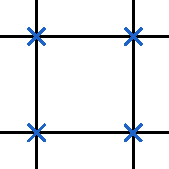
\includegraphics[width=.8\textwidth]{img/chapter4/the_method_grid_zoomed.pdf}};
                \draw[fill, color=ugent_blauw] (2.7,2) circle [radius=2pt] node[above right] {\Large ?};
            \end{tikzpicture}
        \end{center}
    \end{minipage}
    \hfill
    \begin{minipage}{.49\textwidth}
        \begin{center}
            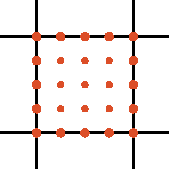
\includegraphics[width=.8\textwidth]{img/chapter4/the_method_grid_interpolate.pdf}
        \end{center}
    \end{minipage}
    \caption{On the left: a closer look at an internal rectangle from figure \ref{fig:woven_method_grid}. On the right: the points calculated with a small finite difference approximation.}\label{fig:c4_new_method_zoomed_in}
\end{figure}

But almost all values in the domain $\Omega$ are not contained on any of these lines. It is not trivial how one would now, from the results $\vb{c_x}$ and $\vb{c_y}$ from the matrix problem reconstruct the eigenfunction $\psi(x, y)$ in such a general point. Let us simplify the problem by only considering a rectangle between two consecutive grid lines, in both the x- and y-direction. The left side of figure \ref{fig:c4_new_method_zoomed_in} contains such a single rectangle. The question now is to reconstruct the eigenfunction on this rectangle, given its value on the whole boundary. Because we have to approximate an unknown function, given the values on a fixed number of points, interpolation comes to mind. As a first idea, we have tried building a polynomial basis to interpolate the eigenfunction with nodes on the boundary of such a rectangle.

\begin{figure}
    \begin{center}
        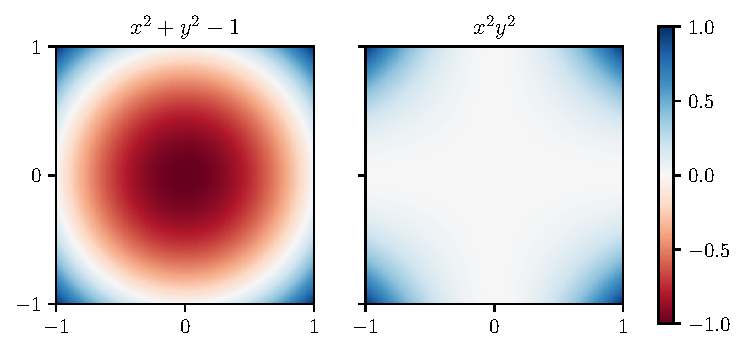
\includegraphics[width=1\textwidth]{img/chapter4/nm_interpolation.pdf}
    \end{center}
    \caption{Two different fourth degree polynomial functions with the same value on the boundary of the region $[-1, 1] \times [-1, 1]$.}\label{fig:c4_interpolation_boundary issue}
\end{figure}

The most natural $k$-degree polynomial basis to consider are for all $i, j$ the polynomials $x^i y^j$ with $i + j \leq k$. For $k = 4$, for example, this yields:
$$
    1\text{, } y\text{, } y^2\text{, } y^3\text{, } y^4\text{, } x\text{, } x y\text{, } x y^2\text{, } x y^3\text{, } x^2\text{, } x^2 y\text{, } x^2 y^2\text{, } x^3\text{, } x^3 y\text{ and } x^4\text{.}
$$
And this basis already highlights one of the fundamental issues with this approach. In figure \ref{fig:c4_interpolation_boundary issue} two different linear combinations of basis functions are plotted: $x^2 + y^2 -1$ and $x^2y^2$. Clearly, these functions are different. Yet, their value on the boundary of the unit square is identical. This indicates that it will not be possible to reconstruct the eigenfunction by using polynomial basis functions based upon only values from the boundary alone.

To be able to calculate an interpolating polynomial uniquely we also require values in the interior of the domain. The vectors $\vb{c_x}$ or $\vb{c_y}$ provide the value of the eigenfunction on the boundary of the small internal rectangle. They tell us nothing about the value of the eigenfuntion in the interior. But, on this internal rectangle $\Omega_{i, j} = [x_i, x_{i+1}] \times [y_j, y_{j+1}]$ we know that the eigenfunction $\psi(x, y)$ satisfies the Schrödinger-like equation
\begin{equation}\label{equ:c4_interpolation_schrodinger}
    -\nabla^2 \psi(x, y) + V(x, y) \psi(x, y) = E \psi(x, y)
\end{equation}
with $E$ fixed and boundary conditions:
\begin{align*}
    \psi(x_i, y)                 & = \sum_{k=0}^\infty c_k^{(x_i)} \beta_k^{(x_i)}(y)\text{,}          \\
    \psi(x_{i+1}, y)             & = \sum_{k=0}^\infty c_k^{(x_{i+1})} \beta_k^{(x_{i+1})}(y)\text{,}  \\
    \psi(x, y_j)                 & = \sum_{k=0}^\infty c_k^{(y_j)} \beta_k^{(y_j)}(x)                  \\
    \text{and } \psi(x, y_{j+1}) & = \sum_{k=0}^\infty c_k^{(y_{j+1})} \beta_k^{(y_{j+1})}(x) \text{.}
\end{align*}

Using this, we place a $K \times K$ grid on this small rectangular domain $\Omega_{i, j}$, as in the right-hand side of figure \ref{fig:c4_new_method_zoomed_in}. The grid points can now be described as $x_i = x^{(i)}_0$, $x^{(i)}_1$, $\dots$, $x^{(i)}_m$, $\dots$, $x^{(i)}_K = x_{i+1}$, and analogous for $y$: $y_j = y^{(j)}_0$, $y^{(j)}_1$, $\dots$, $y^{(j)}_n$, $\dots$, $y^{(j)}_K = y_{j+1}$. This allows the eigenfunction $\psi(x, y)$ to be approximated in each of these points by:
$$
    \psi^{(i,j)}_{m,n} \approx \psi(x^{(i)}_m, y^{(j)}_n) \quad \text{ for each $m, n \in \{0, 1, \dots, K\}$.}
$$
With this notation in hand, equation \ref{equ:c4_interpolation_schrodinger} can be approximated in each grid point by a finite difference approximation. Because $\Omega_{i,j}$ is only a small part of the total domain $\Omega$, the grid size $K$ may be chosen relatively small, without a penalty on accuracy. In our case, we found that fixing $K = 4$ gives satisfactory results, without too much computational overhead. So for the following discussion about a finite difference approximation on $\Omega_{i,j}$, we assume $K = 4$.

Because only a relatively small grid is used, the finite difference scheme should be as accurate as possible, without making any assumptions on points outside $\Omega_{i,j}$. Denote with $f''_0$ the value we want to approximate on an equidistant grid on which the function in question takes the values $\dots, f_{-2}, f_{-1}, f_{0}, f_{1}, f_{2}, \dots$ around the central point. The finite difference approximation can be written as
$$
    f''_0 \approx \sum_{i = a}^{b} \alpha_i f_i
$$
with appropriate choices for $a$ and $b$ such each $f_i$ lies within the grid of approximations. The relevant five-point formula we will be using are provided in the following table.

\begin{center}
    \begin{tabular}{@{}ccc|c|ccc@{}}
        $-3$                               & $-2$            & $-1$            & $0$            & $1$             & $2$             & $3$             \\ \hline
        \rule{0pt}{3ex}                    &                 & $\frac{11}{12}$ & $\frac{-5}{3}$ & $\frac{1}{2}$   & $\frac{1}{3}$   & $\frac{-1}{12}$ \\
        \rule{0pt}{3ex}                    & $\frac{-1}{12}$ & $\frac{4}{3}$   & $\frac{-5}{2}$ & $\frac{4}{3}$   & $\frac{-1}{12}$ &                 \\
        \rule{0pt}{3ex}    $\frac{-1}{12}$ & $\frac{1}{3}$   & $\frac{1}{2}$   & $\frac{-5}{3}$ & $\frac{11}{12}$ &                 &
    \end{tabular}
\end{center}

Let us, for ease of notation, summarize these values into the following matrix:
$$
    \vb{D} = \begin{pmatrix}
        0                             & 0            & 0            & 0            & 0             \\
        \rule{0pt}{3ex} \frac{11}{12} & \frac{-5}{3} & \frac{1}{2}  & \frac{1}{3}  & \frac{-1}{12} \\
        \rule{0pt}{3ex} \frac{-1}{12} & \frac{4}{3}  & \frac{-5}{2} & \frac{4}{3}  & \frac{-1}{12} \\
        \rule{0pt}{3ex} \frac{-1}{12} & \frac{1}{3}  & \frac{1}{2}  & \frac{-5}{3} & \frac{11}{12} \\
        0                             & 0            & 0            & 0            & 0
    \end{pmatrix}\text{.}
$$
With this finite difference approximation \eqref{equ:c4_interpolation_schrodinger} can now be approximated as a nine-dimensional linear system: for each $m, n \in \{1,2,3\}$:
$$
    \begin{cases}
        \qquad\vdots                                                                                                                                                                                                 \\
        {\displaystyle \sum_{l=0}^4 \frac{D_{m, l}}{\Delta x_i^2}\psi^{(i,j)}_{l, n} + \sum_{l=0}^4 \frac{D_{n, l}}{\Delta y_j^2}\psi^{(i,j)}_{m, l} =  \left(V(x^{(i)}_m, y^{(j)}_n) - E\right)\psi^{(i,j)}_{m, n}} \\
        \qquad\vdots
    \end{cases}
$$
The nine unknown variables are $\psi^{(i, j)}_{m, n}$ for $m, n \in \{1,2,3\}$. The step sizes $\Delta x_i$ and $\Delta x_j$ are defined as $\left(x_{i+1} - x_{i}\right) / K$ and $\left(y_{i+1} - y_{i}\right) / K$ respectively. Notice that for all $m, n \in \{0,1,\dots, K\}$, if any of $m, n \in \{0, 4\}$ the values $\psi^{(i, j)}_{m, n}$ are known, as they can be computed as the boundary values.

This relatively small linear system can now be numerically solved to obtain values of the eigenfunction within the small rectangle $\Omega_{i,j}$. On the right-hand side of figure \ref{fig:c4_new_method_zoomed_in}, all red dots are now computed values and can be used to construct a polynomial interpolation. As a basis we have chosen the 25 functions: $x^i y^j$ for all $i,j \in \{0,1,2,3,4\}$.


\subsubsection{Alternative methods}

Throughout the development of an algorithm to compute values of the eigenfunctions, we have considered many other methods for the computation of these eigenfunctions on an interior rectangle as well. In this section we will acknowledge some of these alternatives, together with their strengths and weaknesses. To motivate our final idea of solving a tiny Schrodinger-like problem to find interior points to interpolate through, a modest numerical comparison will be studied.

\paragraph{Interpolation through only boundary points} Previously, we stated that the functions $x^2 + y^2 - 1$ and $x^2 y^2$ have an identical boundary on the square $[-1, 1] \times [-1, 1]$. Also recall figure \ref{fig:c4_interpolation_boundary issue}. This non-uniqueness can be solved by only considering polynomials with a total degree strictly less than four:
$$
    1, x, y, x^2, xy, y^2, x^3, x^2 y, x y^2 \text{ and } y^3\text{.}
$$
These ten functions can now be used as an interpolation basis. For this we choose ten points on the boundary of the internal rectangle. Or, we choose more points and use a least squares approximation.

\todo{Interpolation up to cubic functions}

\todo{Interpolation over different small rectangles}

\todo{$K > 4$, trade off between runtime and accuracy}

\subsubsection{Non-rectangular domains}

\todo{Non-rectangular domains}

\subsection{Numerical experiments}

When developing a new method it is instrumental these are well tested. This inescapably means that the program should be run on many problems with a wide variety of settings. Doing this thoroughly and consistently after code changes can be a cumbersome task. Knowing this, we have from the very first versions onwards included many automatic tests. On every code change, these tests would run on all supported platforms (Linux, Windows and macOS) to verify that our changes still produce sufficiently accurate results for the considered problems. For the development of this new method we continuously test the harmonic oscillator, the Hénon-Heiles potential and the quartic oscillator (\ref{sec:c4_numerical_harmonic} and \ref{sec:c4_numerical_henon_heiles}) on simple rectangular domains, the zero potential (\ref{sec:c4_numerical_zero}) on a rectangular and circular domain and Ixaru's potential on a rectangular, circular and a $45\degree$ rotated rectangle. All tests are conducted in \texttt{double}-precision and most problems are also tested in de extended \texttt{long double} datatype.

These automated tests are extremely valuable during development to quickly notice regressions. But for a thorough mathematical analysis more work is required. In this section we will provide many graphs and figures to evaluate the accuracy of our method. The evaluation of the runtime performance is another can of worms which will be treated in section \ref{sec:c4_nm_vs_fd}.

\subsubsection{Harmonic oscillator}\label{sec:c4_numerical_harmonic}

Following section \ref{sec:c4_fd_numerical}, the first example we will consider is the harmonic oscillator with equation
\begin{equation}\label{equ:c4_nm_harmonic}
    -\nabla^2 \psi(x, y) + \left(x^2 + y^2\right) \psi(x, y) = E \psi(x, y)
\end{equation}
on the domain $[\numprint{-9.5}, \numprint{9.5}] \times [\numprint{-9.5}, \numprint{9.5}]$ with homogeneous Dirichlet boundary conditions.

\begin{figure}
    \begin{center}
        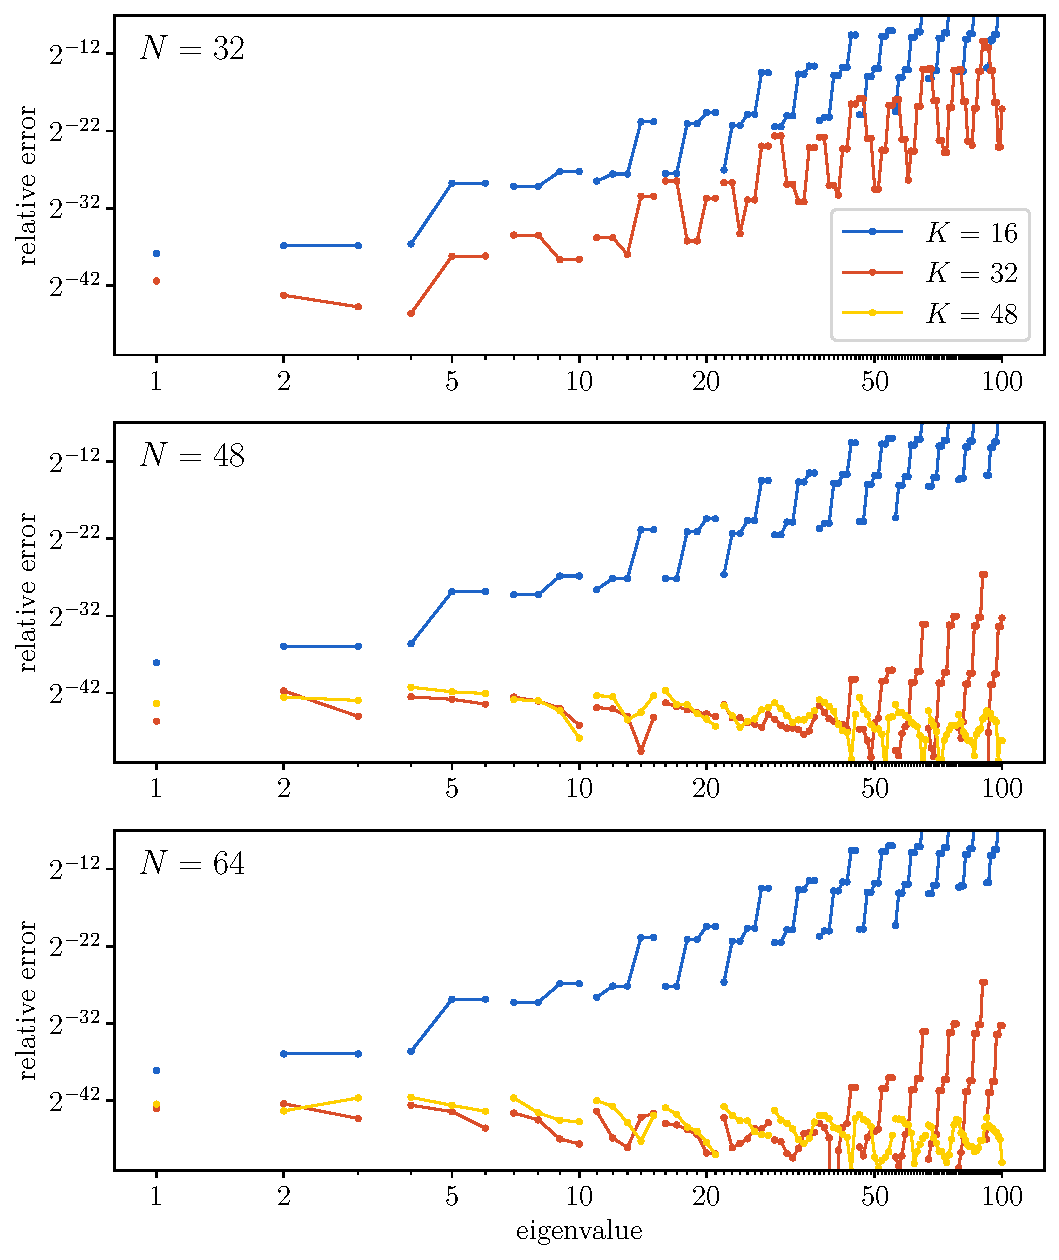
\includegraphics[width=\textwidth]{img/chapter4/nm_test_harmonic.pdf}
    \end{center}
    \caption{These graphs display the relative error of each of the first $100$ eigenvalues of the harmonic oscillator \eqref{equ:c4_nm_harmonic} on a rectangular domain $[-9.5,9.5]\times[-9.5, 9.5]$, computed for different grid sizes $N$ and basis sizes $K$. Repeated eigenvalues are connected.}
    \label{fig:c4_nm_harmonic_rectangle}
\end{figure}

In our algorithm there are two main variables to experiment with. The first, most obvious one, is the density of the used grid. This density lies in line with the grid approximation of the method that uses a finite difference approximation. In our method the size of the involved matrices, and thus the runtime, is directly proportional to the total number of grid points. Being able to use a less dense grid would therefor bring a significant computational benefit to the table.

The second parameter we can tweak is the number of basis functions on each of the grid lines. On each grid line, in both directions, \matslise needs to compute these basis functions. This computation requires, of course, a part of the runtime. In a very crude analysis we can take a look at the computational complexity of both operations. Assume there are $N$ grid lines in both directions. This yields $N^2$ grid points, and $2N$ grid lines. On each of these lines we compute $K \leq N$ basis functions, thus the computational overhead of the many one-dimensional problems is $\OO(K N)$. For the computation of the eigenvalues of the two-dimensional problem, the analysis is more nuanced. Finding accurate and reliable complexity estimates is a more difficult than one would expect. The restarted Arnoldi procedure (without shift-Invert), has a complexity of $\OO(k^2 n)$ when $k$ eigenvalues are requested for a sufficiently sparse $n \times n$ matrix\cite{lee_k2n_2009}. If the linear operator has a dense operation, this dominates the complexity $\OO(k n^2)$. In our case, we support a shift-invert scheme. In this scheme solving the sparse system is definitely something to take into account. \Eigen's built-in methods are based upon techniques from \superlu{}\cite{demmel_supernodal_1999,li_overview_2005}. In the performance analysis of this software, the authors provide a detailed overview of which properties have an impact on performance. An important property which contribute to the runtime is the structure of the matrix. If the non-zero elements of the involved matrix are so situated that the algorithm can exploit it, it helps the computational cost. It is not known whether our matrix has an exploitable structure or not. It would be surprising if our matrix had the perfect structure, independent of the size and shape of the domain.

In summary, a first complexity analysis of our method indicates that the one-dimensional problems have a complexity of $\OO(K N)$ and solving the matrix eigenvalue problem has a complexity of at least $\OO(k N^2)$. One has to be wary to only rely on a theoretical analysis to conclude that solving the one-dimensional problems has a negligible computational cost. In section \ref{sec:c4_nm_vs_fd} we will conduct a thorough analysis of the runtime of our method. For now, we will focus on numerical accuracy.

Figure \ref{fig:c4_nm_harmonic_rectangle} contains three graphs illustrating how the two main variables (grid size and basis size) work together to obtain accurate results. For this figure three different basis sizes were considered $K = 16$, $K = 32$ and $K = 48$. As grid sizes we have chosen $N = 32$, $N = 48$ and $N=64$. Notice that $N = 32$ and $K = 48$ was omitted from the figure as these give exactly the same results as $N = 32$ and $K = 32$, due to the limitation that the number of basis functions can never exceed the number of grid points on the relevant grid line.

Upon close inspection of the comparison of figure \ref{fig:c4_nm_harmonic_rectangle} with figure \ref{fig:c4_fd_harmonic}, we notice that our new method is able to reach the same accuracy with only a grid size of $48$ (with $48$ basis functions). This is considerably less than the required grid size of $100$ with spacing $h = 0.19$ when using the finite difference scheme.

\begin{figure}
    \begin{center}
        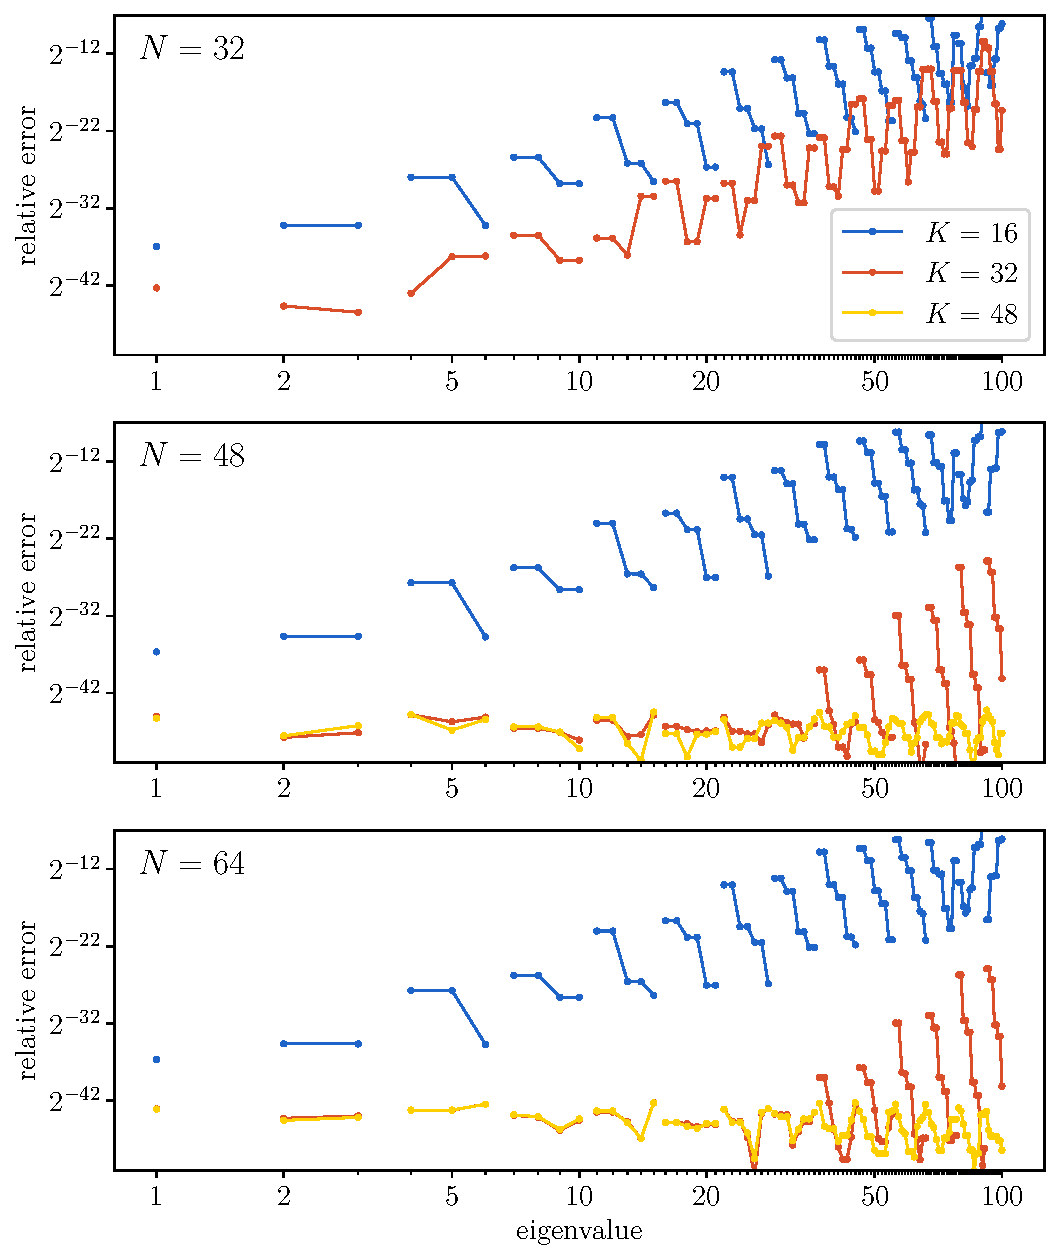
\includegraphics[width=\textwidth]{img/chapter4/nm_test_harmonic_disc.pdf}
    \end{center}
    \caption{These graphs display the relative error of each of the first $100$ eigenvalues of the harmonic oscillator \eqref{equ:c4_nm_harmonic} on the disc around $\vb{0}$ with radius $9.5$, computed for different grid sizes $N$ and maximal basis sizes $K \leq N$. On every line, the used basis size will be limited to the number of grid points on that line. Repeated eigenvalues are connected.}
    \label{fig:c4_nm_harmonic_disc}
\end{figure}

As a second, highly related experiment we try the harmonic oscillator, equation \eqref{equ:c4_nm_harmonic} on a circular domain around $(0, 0)$ with radius $9.5$. In principle, this is the same problem as before. But in practice, solving Schrödinger problems on non-rectangular domains was not at all possible with other grid-based methods.

Because we have constructed this method with non-rectangular domains in mind, ours is able to tackle these more exotic problems. Figure \ref{fig:c4_nm_harmonic_disc} answers for this problem the most important question: are the results accurate? The graphs displayed in this figure are calculated in the same way as figure \ref{fig:c4_nm_harmonic_rectangle}. Three different grid sizes and three different maximal basis sizes are considered. Notice that we used the term \emph{maximal} basis size. For non-rectangular domains the number of grid points per grid line varies. Grid lines close to the boundary are short chords containing only a few grid points. As the number of points limits the size of the basis, the true basis size has to vary as well. For our algorithm it is still valuable to place an upper bound on the basis size, especially for those lines that run through the middle of the domain, with many containing grid points.

\begin{figure}
    \begin{center}
        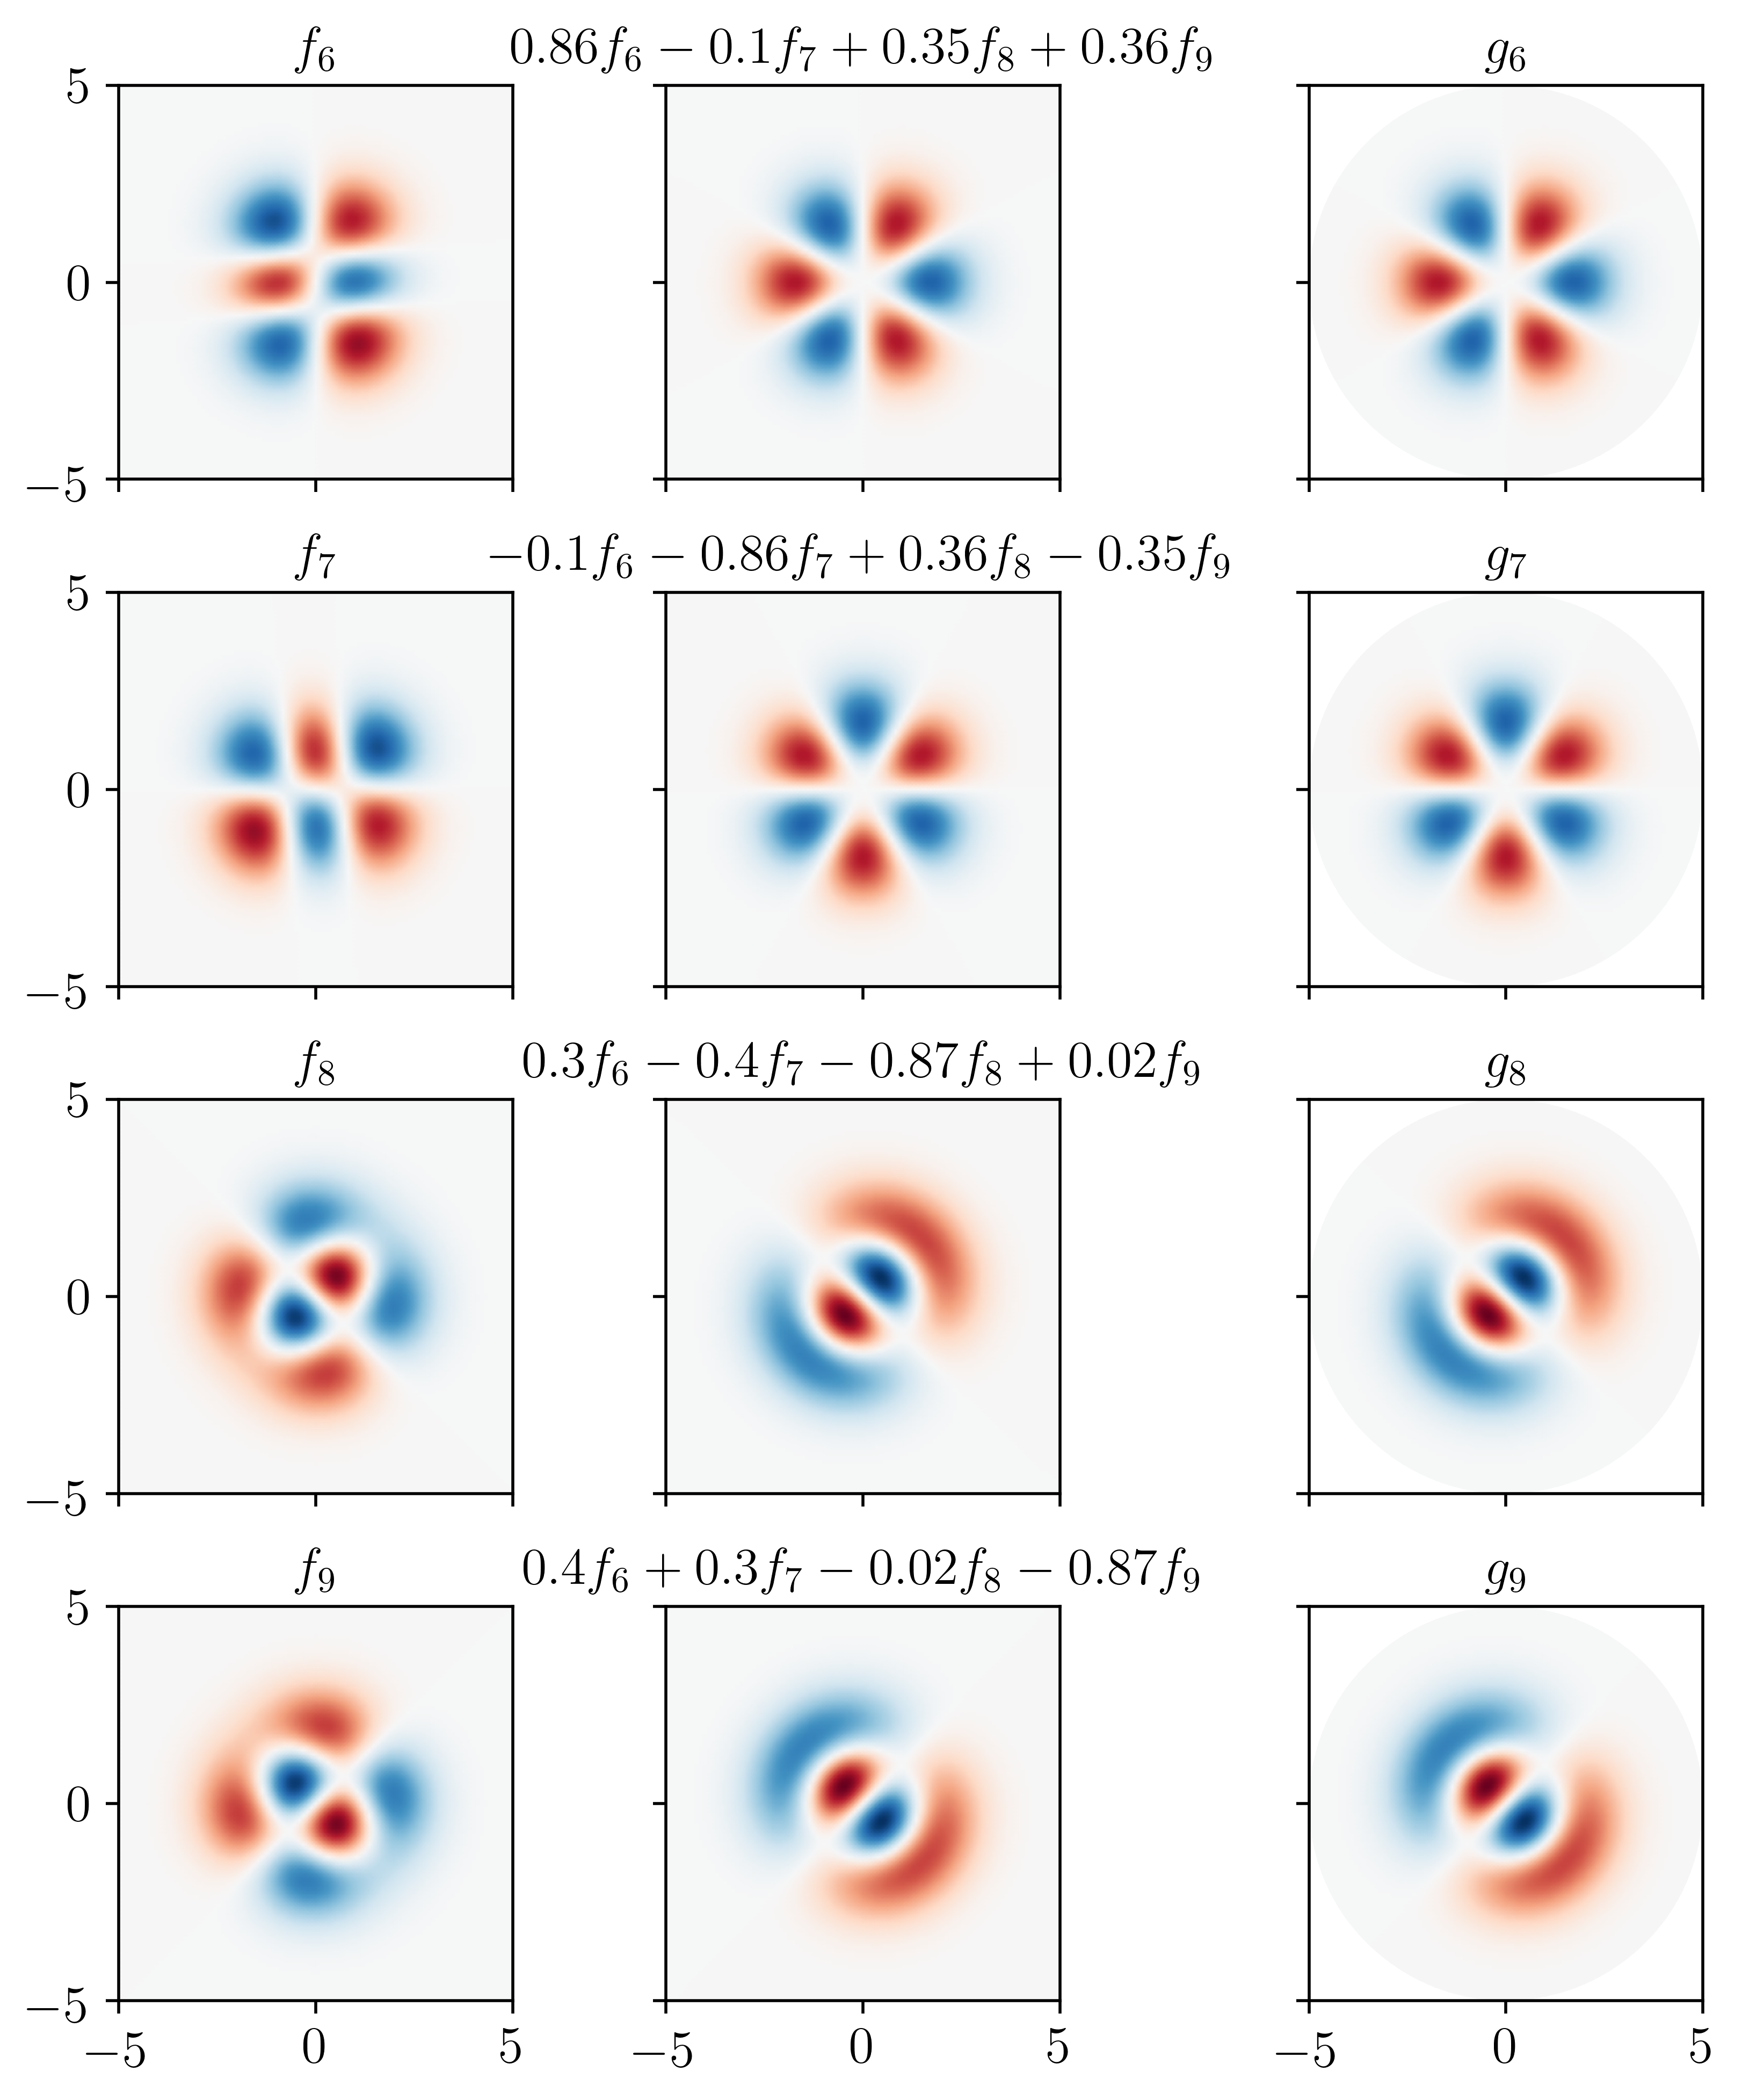
\includegraphics[width=\textwidth]{img/chapter4/nm_test_harmonic_eigenfunctions.png}
    \end{center}
    \caption{Left: four eigenfunctions with the same eigenvalue of the harmonic oscillator on the rectangular domain $[-5, 5]$. Right: the corresponding eigenfunctions on the circular domain with radius $5$. Middle: linear combinations of the left eigenfunctions are chosen such that they equal the right eigenfunctions.}
    \label{fig:c4_nm_harmonic_eigenfunctions}
\end{figure}

The results of figure \ref{fig:c4_nm_harmonic_disc} are eerily similar to those of figure \ref{fig:c4_nm_harmonic_rectangle}. For the harmonic oscillator the domain seems to have no effect on the accuracy of the method. This can be explained by the fact that for all eigenfunctions $f(\vb{x})$: $\lim_{\|\vb{x}\| \to +\infty} f(\vb{x}) = 0$. As a consequence this means that once the domain is sufficiently large the boundary, and corresponding boundary conditions, become less and less important. One of the great benefits of considering this circular domain is its size. For example, if $N = 64$ the rectangular domain has $4096$ grid points. The circular domain on the other hand, only has $3300$ grid points. This reduction in grid points makes the involved matrices smaller, and therefor reduces the computational cost.

As a last visual experiment with the harmonic oscillator, we will take a look at the eigenfunctions. As a reminder: the true eigenfunctions of the two-dimensional harmonic oscillator are:
$$
    2, 4, 4, 6, 6, 6, 8, 8, 8, 8, 10, 10, 10, 10, 10, 12, \dots
$$
Figure \ref{fig:c4_nm_harmonic_eigenfunctions} plots a basis for all eigenfunctions corresponding to eigenvalue $\lambda_6 = \lambda_7 = \lambda_8 = \lambda_9 = 8$. In the left-most column the basis for the eigenfunctions on the square domain $[-5, 5] \times [-5, 5]$ can be seen, and in the right-most column the basis found on a circular domain around zero with radius $5$. We have opted here for a smaller domain, not because of computational cost, on the larger domain these eigenfunctions can be drawn just as quickly. But, because of visual usefulness. On a larger domain, the interesting center part of the image would be a lot smaller and thus less visible.

Upon a first viewing of these eigenfunctions (left and right columns) one may be surprised that these are different. But, as the eigenspace corresponding to eigenvalue $8$ is multidimensional the basis is no longer unique. To be able to compare these results we have introduced the middle column. Here, a linear combination of basis functions from the rectangular domain is calculated such that we obtain the same basis functions as found on the circular domain. This illustrates some of the challenges when trying to compare or numerically verify eigenfunctions.

\subsubsection{Zero potential}\label{sec:c4_numerical_zero}

Analogous to section \ref{sec:c4_fd_numerical}, the next example we will study is the zero potential. Here the Schrödinger equation simplifies to:
$$
    -\nabla^2 \phi(x, y) = \lambda\phi(x, y)
$$
on the domain $\Omega$, with homogeneous Dirichlet boundary conditions.

If the domain $\Omega$ is the rectangle $[0, \pi] \times [0, \pi]$ exact solutions can be obtained with separation of variables. This gives $\forall i, j \in \Nplus$ that $i^2 + j^2$ is an eigenvalue of this Schrödinger problem with corresponding eigenfunction $\phi(x, y) = \sin(i x)\sin(j y)$.

\begin{figure}
    \begin{center}
        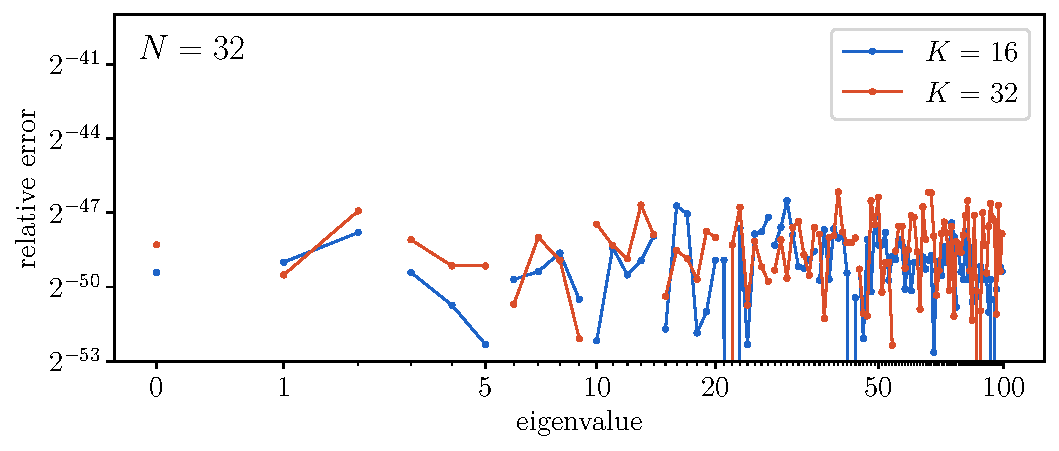
\includegraphics[width=\textwidth]{img/chapter4/nm_test_zero_rectangle.pdf}
    \end{center}
    \caption{This graph displays the results of our new method for the zero potential on the square $[0, \pi] \times [0, \pi]$, for a fixed grid size of $N = 32$ and a varying basis size. Notice the zoomed in y-axis, close to the machine precision of $2^{-53}$.}
    \label{fig:c4_nm_zero_test_rectangle}
\end{figure}

In figure \ref{fig:c4_nm_zero_test_rectangle} the results for this problem are visualized. Unsurprisingly, our method works extremely well for this. The main reason can be found in the fact that the basis functions \matslise calculates on each line are exactly $\sin(x)$, $\sin(2x)$, $\sin(3x)$\dots and analogous for $y$. These functions are able to exactly represent the true eigenfunctions $\sin(i x)\sin(j y)$ on each line.

\begin{figure}
    \begin{center}
        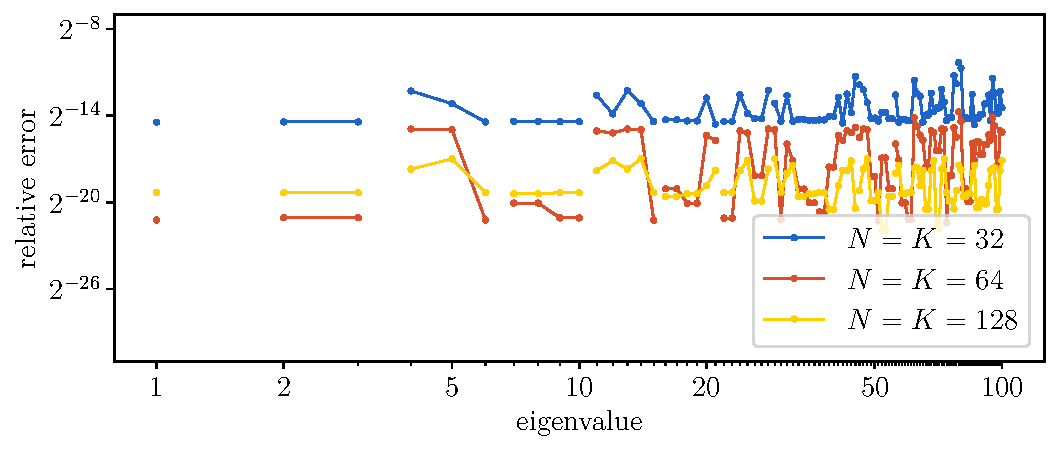
\includegraphics[width=\textwidth]{img/chapter4/nm_test_zero_disc.pdf}
    \end{center}
    \caption{This graph displays the results of our new method for the zero potential on the circular domain around $(0, 0)$ with radius $5$, for varying grid and basis sizes. Notice the shifted y-axis, to larger errors.}
    \label{fig:c4_nm_zero_test_disc}
\end{figure}

For non-rectangular domains with the zero potential, the story is different. Let us consider the Schrödinger equation with the zero potential and the circular domain around $(0, 0)$ with radius $1$ and homogeneous Dirichlet boundary conditions. The exact eigenvalues are known as the squares of the roots of the Bessel functions. See section \ref{sec:c3_eigenvalues_wrt_domain_analysis} for the full symbolic calculation.

The relative errors of the first hundred eigenvalues found with our new method are shown in figure \ref{fig:c4_nm_zero_test_disc}. We have tested this with the grid size and maximal basis size both equal to $32$, $64$ or $128$. The results are less impressive than for rectangular domains as the maximal accuracy reached is somewhere around $10^{-6}$. But nevertheless being able to compute these values at all is quite unique.


\subsubsection{Hénon-Heiles potential}\label{sec:c4_numerical_henon_heiles}

Another often used test problem is the Hénon-Heiles system. In the context of time-independent two-dimensional Schrödinger equations the potential in question is given as:
$$
    V(x, y) = x^2 + y^2 + \frac{3\sqrt{5}}{10}(3 x y^2 - x^3)\text{.}
$$
For a detailed analysis of this potential we refer back to section \ref{sec:c3_experiment_henon}.

\begin{figure}
    \begin{center}
        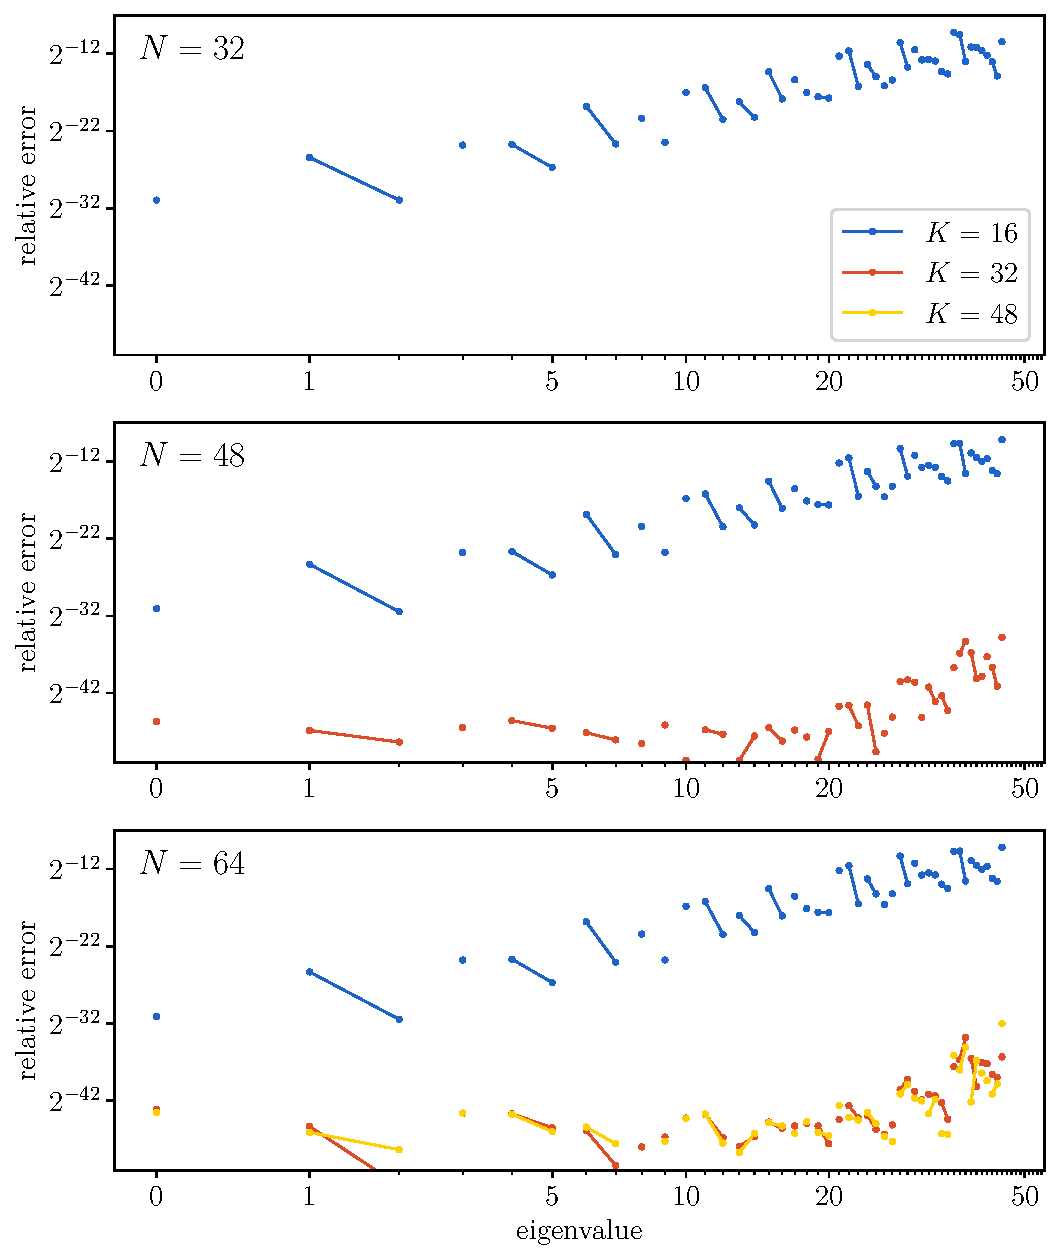
\includegraphics[width=\textwidth]{img/chapter4/nm_test_henon.pdf}
    \end{center}
    \caption{These graphs display the relative errors when we compare the results from our method with those from \cite{wang_new_2009} for the Hénon-Heiles system on the domain $[-10, 10]\times[-10, 10]$. For the parameters $N = K = 32$ and $N = K = 48$, our method found some physically nonsensical eigenvalues and therefor are missing from the plots.}
    \label{fig:c4_nm_henon_test}
\end{figure}

In \cite{wang_new_2009}, the authors remark to take care when choosing the size of the domain. This should not be too small to allow the eigenfunctions to converge to zero on the boundary. But it should neither be too large, because this can generate some physically nonsensical eigenvalues. They take as domain $[-10, 10] \times [-10, 10]$ and leave it at that. Looking at the available literature about this problem we find for example \cite{davis_semiclassical_1979}. Here, the proposed method does not use a clear defined boundary, but uses infinite basis functions. But, the interesting regions of these basis functions are only present in a radius, much smaller than $10$, around zero. \cite{braun_efficient_1996} limits their grid to a $[-6, 6] \times [-6, 6]$ domain. And in \cite{baeyens_improvements_2022}, we follow \cite{braun_efficient_1996}. For this experiment we will also take a $[-10, 10] \times [-10, 10]$ domain.

In figure \ref{fig:c4_nm_henon_test} the relative errors obtained with our method our displayed for this experiment. We used the results from \cite{wang_new_2009} as reference. Before analyzing these results we need to mention that for $N = K = 32$ and $N = K = 48$ our method found many nonsensical small eigenvalues. We know that they have no physical meaning because the corresponding eigenfunctions are only non-zero inside the valleys at the boundary. These unwanted eigenvalues disappear if the domain would be a little smaller, such that it no longer contains any valleys at the boundary.

Ignoring these special cases allows us to interpret the graphs from figure \ref{fig:c4_nm_henon_test}. Even on a small grid $N = 48$ we are able to accurately determine the eigenvalues. We also see that for the high eigenvalues increasing the grid size or basis size seems to have no effect. This is unexpected and seems to indicate that maybe the reference values are not perfect. The relative error for these high eigenvalues is $< 2^{-32} \approx 10^{-10}$ which is nonetheless extremely accurate.

\subsubsection{Ixaru's potential}\label{sec:c4_numerical_ixaru}



\subsection{Comparing run time with the finite difference method}\label{sec:c4_nm_vs_fd}

\section{Some ideas for a utopian method}\label{c4:sec_utopy}

In the introduction of this chapter we briefly discussed what a perfect method for time independent Schrödinger equations may be. It should be a method which is fast and accurate, of course. More specifically, its accuracy should not degrade upon requesting higher eigenvalues. Even if ridiculously high eigenvalues are required. But, ideally, this guaranteed accuracy should not come with the cost of increased run time. Requesting the first five eigenvalues should be (approximately) as fast as requesting the five eigenvalues larger than one million for example.

In this section, I want to give an overview of the ideas and experiments I explored in the past few years. This section will not be written as a scientific paper. It will not contain absolute truths. It will not allege to have any certainties. This section will contain many of my mathematical feelings, unverified, uncensored, and definitely not peer reviewed. And, I will try highlight in which ideas I still see merit, and with which ideas I have run into a dead end.

Before diving into my mathematical ramblings, I need to give you some caveats: I have not read every article about the topics described here. I do not know all intricacies of developing numerical methods. And I see myself as an applied mathematician\footnote{This is not an apology, I am a proud (and proudly) applied mathematician. But, my background influences how I practice mathematics. And in this section in particular this is important to keep in mind when following along with my thoughts.}, so I prefer numerical experiments and testing a hypothesis over strong mathematical rigor and watertight proofs. Still, I believe myself to be somewhat qualified to write about numerical methods for two-dimensional time independent Schrödinger equations, as I spent the previous (almost) six years of my professional time developing such methods myself. But, if you have invested yourself in any of the topics we will cover here, and you find me to be unjustly negative or unfairly harsh, I really do want to apologize in advance for that. It is not my intention to write theories off. It is not my intention to declare topics a waste of time. All things I write here are and will be my experience with these topics, in and only in the context of numerical methods for the two-dimensional time independent Schrödinger equation.

\subsection{Preliminary ideas}

\subsubsection{Exponential fitting}

The first topic I want to cover here is already controversial. My research group and in particular my promotor are already studying exponential fitting for over three decades. They were able to successfully use this technique countless times in various applications. And, I know, as a young researcher, even younger than they have been researching this topic even, it is quite pretentious to make statements about this topic. But my promotor and I have worked sufficiently close together, that he knows me to make some statement I better should not have. Let this subsection be such a statement.

The general idea of exponential fitting is to develop methods which are specifically tuned to be accurate for exponential and oscillatory function of certain frequencies. They have been successfully applied to numerical differentiation, quadrature formulas and ordinary differential equations (linear multistep methods and Runge-Kutta methods)\cite{ixaru_exponential_2004}. For the more recent advances we refer to \cite{paternoster_present_2012}. The success of this technique can not be denied.

Yet, my relationship with exponential fitting has been rocky. Most importantly, this thesis could not have come to fruition without them. The constant perturbation methods, and in particular \matslise, are exponentially fitted methods. The extreme accuracies reached for the one-dimensional problem are only possible because for each energy the specifically tuned $\eta$-functions take exactly the important frequencies into account.

On the other hand, when we tried to use exponentially fitted quadrature formulas for the computation of the potential matrix $\vb{V}^{(k)}(y)$ in section \ref{sec:c3_calculate_vk}, the results were less than ideal. It was already quite the challenge to determine to which frequencies these formulae should be tuned. Because these quadrature formulae should be computed for many possible eigenvalues and for all sectors of the domain with a wildly varying potential, the fitted frequencies most definitely could not be constant. So they should be automatically and dynamically computed. In principle this only incurs a small computational overhead. In practice, this was quite difficult to implement. We needed to tune the formulae for different frequencies and many edge-cases arose: what if some of them were close together? What if some functions were exponential and the others trigonometric? Or all exponential? Or none of them? All these question were interconnected, and important. If two frequencies were close together, in the formulae we were dividing two tiny numbers. So the limit had to be taken. In relatively rare cases the resulting quadrature formulae became highly unstable with large negative weights. One of the major issues was that even though these cases were quite rare, they popped up often because we were approximating so many integrals. In short, this instability caused a numerical mess. After this experience, I hope you can understand the hesitation in my love for exponential fitting.

The eigenfunctions of the two-dimensional eigenproblem we are trying to solve are oscillatory, even highly so for large eigenvalues. Therefor, it is natural to think about exponential fitting. But translating this idea into something practical is not straightforward. For ordinary differential systems much research from recent years is available: second order problems\cite{dambrosio_exponentially_2011,}, symplectic methods \cite{vandenberghe_symplectic_2011,wu_explicit_2012}\dots For partial differential equations we have found very little research available. In \cite{zahra_exponentially_2019} the authors develop an exponentially fitted method for the two-dimensional time fractional damped Klein-Gordon equation. Upon construction of the symbolic formulae they use a polynomial basis set together with the following exponential functions, based upon the parameters $\mu, \nu \in \CC$:
$$
    \exp(\pm\mu x \pm\nu y), x\exp(\pm\mu x \pm\nu y), y\exp(\pm\mu x \pm\nu y), x y \exp(\pm\mu x \pm\nu y), \dots
$$
For determining $\mu$ and $\nu$ they propose an algorithm which is able to eliminate the leading term of the error by choosing these parameters appropriately. In our case, using this set of basis functions directly will be far from optimal. For the Schrödinger equation, we have seen that the frequency of the oscillations is highly dependent on the value of the potential. Where in the domain the potential is low, the eigenfunction will strongly oscillate, where the potential is higher the oscillations will slow down, and where the potential is even higher than the energy there will be no oscillations at all, and we have an exponential behavior. So in a certain sense, the values of $\mu$ and $\nu$ should dependent upon the energy and upon the value of the potential, and by extension thus the location $x, y$ in the domain.


\subsubsection{Piecewise constant approximations}

\todo{Canosa and De Oliveira first ideas, high level overview and quick sketch for 2D}

\subsubsection{Constant perturbation}

\todo{Without being negative: why it is secondary to the constant approximation}

\subsubsection{Shooting}

\todo{Shooting vs direct methods, why we need shooting for high eigenvalues}

\subsubsection{Finding eigenvalues within an order of magnitude}

\todo{Like Prüfer}

\subsection{The main idea}

\todo{Some formulas, boundary conditions, propagation, CP?}



\stopchapter


% !TeX root = chapter_closing_remarks.tex
% !TeX root = thesis.tex
\ifdefined\UtilIncluded
  \renewcommand{\startchapter}[1]{}
  \renewcommand{\stopchapter}{}
  \renewcommand{\undefinedlabel}[2]{}
\else

\newcommand{\startchapter}[1]{\begin{document}\setcounter{chapter}{#1}\addtocounter{chapter}{-1}}
\newcommand{\stopchapter}{\printbibliography[title=Bibliography,heading=bibintoc]\end{document}}


\documentclass{book}
\usepackage[utf8]{inputenc}


\usepackage{geometry}
\geometry{
  papersize={170mm,240mm},
}

\usepackage{amsfonts,amsmath, amsthm, amssymb, mathtools}
\usepackage{xspace}
\usepackage[hidelinks,bookmarks,pdfusetitle]{hyperref}
\usepackage{listings}
\usepackage[pdftex]{graphicx}
\usepackage{bm}
\usepackage[english]{babel}
\usepackage{caption}
\usepackage{subcaption}
\usepackage[usenames,dvipsnames]{xcolor}
\usepackage{physics}
\usepackage{multicol}
\usepackage{xstring}
\usepackage{pythonhighlight}
\usepackage{parskip}
\usepackage{thmtools}
\usepackage{relsize}
\usepackage{bookmark}
\usepackage{lmodern}
\usepackage{ifthen}
\usepackage{biblatex}
\usepackage{microtype}
\usepackage{csquotes}
\usepackage{numprint}
\usepackage{mleftright}
\npthousandsep{{\ifmmode\mskip2mu\else\hskip0.2em\fi}}
\npdecimalsign{.}

\addbibresource{references.bib}

\newtheorem{theorem}{Theorem}[chapter]
\newtheorem{lemma}[theorem]{Lemma}
\newtheorem{corollary}[theorem]{Corollary}
\newtheorem{definition}[theorem]{Definition}

\DeclareRobustCommand{\oneD}{{1{\relsize{-1}D}}\xspace}
\DeclareRobustCommand{\twoD}{{2{\relsize{-1}D}}\xspace}
\DeclareRobustCommand{\threeD}{{3{\relsize{-1}D}}\xspace}
\DeclareRobustCommand{\cpp}{{{C\nolinebreak[4]\hspace{-.05em}\raisebox{.4ex}{\relsize{-3}\textbf{++}}}\xspace}}
\pdfstringdefDisableCommands{%
  \def\cpp{C++}%
  \def\oneD{1D}%
  \def\twoD{2D}%
  \def\threeD{3D}%
}

\newcommand{\longchapter}[2][]{%
  \chapter[#2]{#2}%
  \ifthenelse{\equal{#1}{}}{}{\chaptermark{#1}}}

\newcommand{\NN}{\mathbb{N}}
\newcommand{\ZZ}{\mathbb{Z}}
\newcommand{\QQ}{\mathbb{Q}}
\newcommand{\QQbar}{\overline{\mathbb{Q}}}
\newcommand{\RR}{\mathbb{R}}
\newcommand{\CC}{\mathbb{C}}

\newcommand{\Eigen}{\texttt{Eigen}}

\newcommand{\sage}{\texttt{sage}\xspace}

\newcommand{\hamiltonian}{\mathcal{H}}

\newcommand{\transposesign}{\intercal}
\newcommand{\transpose}[1]{{#1}^\transposesign}
\newcommand{\adjointsign}{\text{H}}
\newcommand{\adjoint}[1]{{#1}^\adjointsign}

\newcommand{\xmin}{{x_{\text{min}}}}
\newcommand{\xmax}{{x_{\text{max}}}}
\newcommand{\ymin}{{y_{\text{min}}}}
\newcommand{\ymax}{{y_{\text{max}}}}

\newcommand{\Cbottom}{\vb{C}_\text{bottom}}
\newcommand{\Ctop}{\vb{C}_\text{top}}
\newcommand{\ubottom}{\vb{u}_\text{bottom}}
\newcommand{\utop}{\vb{u}_\text{top}}

\DeclareMathOperator{\diag}{diag}
\DeclareMathOperator{\tridiag}{tridiag}
\DeclareMathOperator{\eigs}{eigs}
\DeclareMathOperator*{\argmin}{arg\,min}
\DeclareMathOperator{\Ai}{Ai}
\DeclareMathOperator{\Bi}{Bi}
\DeclareMathOperator{\OO}{\mathcal{O}}

% https://tex.stackexchange.com/a/18192/163747
\makeatletter
\newcommand{\undefinedlabel}[2]{%
  \protected@write \@auxout {}{\string \newlabel {#1}{{#2}{\thepage}{#2}{#1}{}} }%
  \hypertarget{#1}{}
}
\makeatother

\fi
\gdef\UtilIncluded{}


\startchapter{5}

\undefinedlabel{cha:c2}{2}
\undefinedlabel{cha:c3}{3}
\undefinedlabel{cha:c4}{4}
\undefinedlabel{sec:c2_implementation_automatic_testing}{2.x.x.x}
\undefinedlabel{sec:c3_standing_waves_on_disc}{3.x.x.x}
\undefinedlabel{sec:c3_experiment_henon}{3.x.x}
\undefinedlabel{sec:c3_calculate_vk}{3.x.x}
\undefinedlabel{the:c3_counting_eigenvalues}{3.x}
\undefinedlabel{sec:c4_strands}{4.x}
\undefinedlabel{equ:c4_nm_matrix_compact}{4.x}
\undefinedlabel{sec:c4_matrix_least_squares}{4.x.x}

\chapter*{Closing remarks}
\addcontentsline{toc}{chapter}{Closing remarks}

Looking back at this thesis, and the researching years preceding it, fills me with many emotions: both positive, as well as less positive. First and foremost, I am quite proud of the results we were able to achieve. In chapter~\ref{cha:c2}, we have started from a well-established and thoroughly studied technique for one-dimensional Schrödinger equations, and we improved upon known results. Both theoretical and practical advances were made. In chapter~\ref{cha:c3}, we have taken a relatively new technique and build upon it. Our implementation advances the use of this technique with some new features. For these, we took some theoretical strides. One of the results I am most proud of in this thesis is theorem~\ref{the:c3_counting_eigenvalues}. Five years ago, when I implemented this new technique for the first time in \matlab{}, I was disappointed that it was impossible to ensure one has found all eigenvalues in a given range. In my master's thesis I have voiced this missing feature as a possible idea for future work. Privately, my promotor and I were rather pessimistic if this issue could ever be fixed. We believed that this method was too complicated to be able to give any guarantees on the index of eigenvalues. Despite this pessimism, I am proud that we have persevered and developed this new theorem~\ref{the:c3_counting_eigenvalues}.

During the research for chapters~\ref{cha:c2} and~\ref{cha:c3}, at times, I was quite demotivated. Although we were advancing and building improvements, both techniques were not \emph{mine}. I had difficulties finding ownership. The real low-point in my PhD-research was in August 2020. I was browsing through the literature and found an article which was able to solve the two-dimensional Schrödinger equations faster and more accurate than we ever could. Unavoidably, many existential questions were raised. Getting through this \emph{crisis of faith} was definitely not easy. It took some time, but a few long months later, I found renewed inspiration and \emph{goesting}\footnote{This is a very Flemish word. It loosely translates to `with an enthusiastic motivation'.}. In my archives, the earliest draft I can find for ideas for a new method for two-dimensional Schrödinger equations dates from February 2021. And in the subsequent years I have learned that, maybe unsurprisingly, developing a new method is hard. We went through many iterations. In chapter~\ref{cha:c4}, you can read the (for now) final version.


\section*{Looking forward}
\addcontentsline{toc}{section}{Looking forward}

Writing about what the future will bring is, what we would call in Dutch, looking at coffee grounds\footnote{In English, more commonly: reading tea leaves.}. Without sounding overly ambitious: I hope our new method and our implementation may be useful for someone somewhere.

As all things in life, our new method is not perfect. One of the more user-friendly features of our improvements to the method from chapter~\ref{cha:c3}, is the ability to automatically select the needed sector sizes to ensure a requested accuracy. In chapter~\ref{cha:c4}, the grid size is still an open parameter. The relation of this size to the numerical accuracy is not yet thoroughly researched. Also, in section~\ref{sec:c4_strands}, we were adamant that our new technique works on non-uniform grids with varying basis sizes on each grid line. Yet, we studied this only to a limited extent. Ideally, some automatic  grid selection should be implemented. In vague terms, on regions of the domain where the sought eigenfunctions are interesting, the used grid should be denser. Implementing a heuristic for this may be straightforward, but being able to guarantee that a given accuracy is obtained with a particular grid is difficult. Another improvement to this technique may be found in the choice of basis functions on grid lines. On the line $x = x_i$, in chapter~\ref{cha:c4}, we solve a one-dimensional Schrödinger problem with potential $\frac{1}{2} V(x_i, y)$. In each grid point, the value of the potential is split between both intersecting grid lines. In principle, this split does not need to be equal. Maybe other choices can be defended as well.

Besides direct improvements to the method itself, we believe more fundamentally different ideas can be explored. Does the grid need to be square? How can this method be used to solve time-dependent Schrödinger equations\footnote{For one-dimensional time-dependent problems, \matslise{2} is used in~\cite{ledoux_accurate_2014}.}? Can this technique be extended to general linear operators? What changes when solving three-dimensional problems?

Concerning the three-dimensional problem, we have studied some preparatory ideas. Following the two-dimensional method, we place a rectangular grid on the domain, with three grid lines per grid point. As a basis, we could use eigenfunctions of one-dimensional Schrödinger problems with a three-way split of the potential. For example, on the line $x = x_i \land y = y_j$ we solve the one-dimensional Schrödinger problem with potential $\frac{1}{3} V(x_i, y_j, z)$. To find the eigenvalues we have to solve (analogous to~\eqref{equ:c4_nm_matrix_compact})
$$
    \vb{B_x} \vb{\Lambda_x}\vb{c_x} + \vb{B_y} \vb{\Lambda_y}\vb{c_y} + \vb{B_z} \vb{\Lambda_z}\vb{c_z} = E \vb{B_x} \vb{c_x} = E \vb{B_y} \vb{c_y} = E \vb{B_z} \vb{c_z}\text{.}
$$
The technique to solve this equation, as described in section~\ref{sec:c4_matrix_least_squares}, generalizes elegantly for more dimensions. In summary, approximating eigenvalues is quite straightforward. The largest issues we have found in a first exploratory study is the computation of an eigenfunction in arbitrary points. No longer can we use the same trick to solve a much smaller Schrödinger problem with calculated boundary conditions. Eigenfunction solutions are only known upon the grid lines, not on the planer faces of each of the grid cells.

On a more personal note, the researching for and the writing of this thesis has taught me a great deal. Some lessons were a confirmation of things I already knew. For example, I really like solving problems. When a new challenge crosses my path, far too often I think: ``It could not be \emph{that} hard, right?'' And, after spending anything between a few hours and a few years trying to solve the problem, I have to conclude: ``Well, it definitely is that hard.''

One of the other lessons I learned about myself is that I like collaborating. In researching this thesis, it was almost always only my promotor and I. Now, I am very fortunate to get along really well\footnote{Of course, I hope (and do believe) that this is symmetric.} with my promotor. Yet, many times I felt that I was missing some more people to collaborate with, to bounce ideas around with, to just talk with...

The last lesson I want to share is that I easily get distracted with interesting problems. During the past five years, far too many times I was very busy not doing my PhD-research. All these distractions are out of the scope of this text. However, if you, the reader, want to talk with me, and don't know what about, then just ask me something about:
mathematical origami,
plagiarism detection in source code,
sunlight on crop fields for agroforestry,
basins of convergence and Julia sets,
ray tracing in mathematical figures,
hyperbolic geometry (in VR),
the roots of the Littlewood polynomials,
picking numbers in a lottery,
dynamical systems in arbitrary precision,
geodesics and shortest paths over surfaces,
computations in non-commutative quantum algebras,
Keith numbers,
drawing L-systems\dots

As the last paragraph, I want to thank Marnix once again to be my guide during this research, to provide invaluable much appreciated feedback and to give me the freedom to pursue my distractions. But also again, I want to thank Emilie for being my best friend, for listening to all my troubles and for carrying my burdens with me.

\vspace{1cm}

\begin{flushright}
    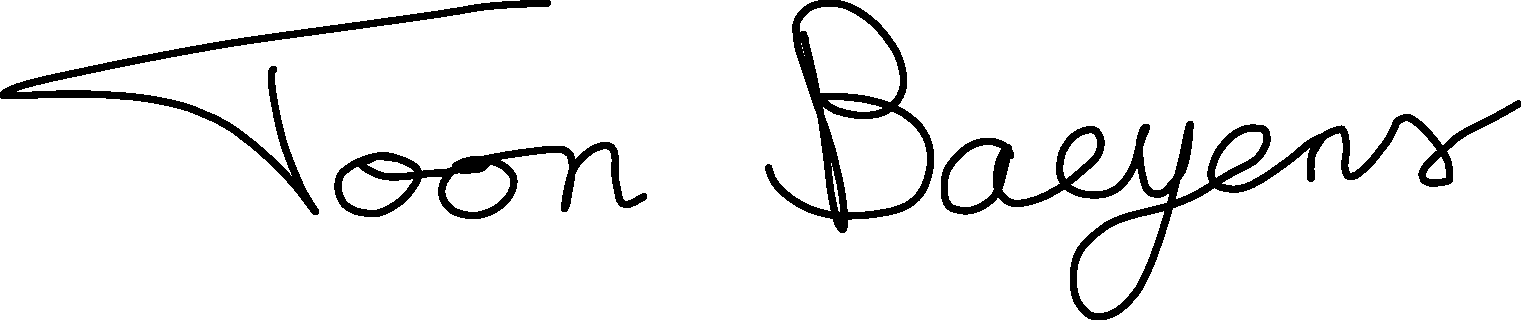
\includegraphics[width=4cm]{img/signature.pdf}\\
    April 2023
\end{flushright}

\stopchapter


\cleardoublepage

\printbibliography[title=Bibliography,heading=bibintoc]

\end{document}
